
\documentclass[12pt,letterpaper]{article}

%---------------------- Codificacion e idioma -------------------------
\usepackage[utf8]{inputenc}
\usepackage[T1]{fontenc}
\usepackage[spanish,es-nodecimaldot,es-noquoting,es-noshorthands,es-tabla,es-nosectiondot]{babel}
\usepackage{lmodern}

%---------------------- Geometria y espaciado -------------------------
\usepackage[letterpaper,top=2.5cm,bottom=2.5cm,left=3cm,right=2.5cm]{geometry}
\usepackage{setspace}
\onehalfspacing
\setlength{\parskip}{0.6em}
\setlength{\parindent}{0pt}

%---------------------- Tablas, listas y graficos ---------------------
\usepackage{amsmath,amssymb}
\usepackage{booktabs}
\usepackage{tabularx}
\usepackage{array}
\usepackage{enumitem}
\usepackage{ragged2e}
\usepackage{graphicx}
\usepackage{float}
\usepackage{longtable}
\usepackage{adjustbox}
% Listados de consultas SQL (capitulo 6)
\usepackage{listings}
\lstdefinestyle{sqlpro}{language=SQL, basicstyle=\ttfamily\footnotesize,
  keywordstyle=\bfseries, columns=fullflexible, keepspaces=true,
  frame=single, framerule=0.3pt, rulecolor=\color{gray},
  xleftmargin=6pt, xrightmargin=6pt, aboveskip=6pt, belowskip=6pt,
  morekeywords={JOIN,ON,HAVING,UNION,REPLACE,VIEW}, literate={á}{{\'a}}1 {é}{{\'e}}1 {í}{{\'i}}1 {ó}{{\'o}}1 {ú}{{\'u}}1 {ñ}{{\~n}}1}
\usepackage{pdflscape}
\usepackage{multirow}
\usepackage{tikz}
\usetikzlibrary{positioning,calc,arrows.meta,backgrounds,shapes.geometric}

\usepackage[hidelinks]{hyperref}

% La plantilla llega hasta el cuarto nivel (p. ej. 3.3.2.1)
\setcounter{secnumdepth}{4}
% Tabla de contenido hasta el tercer nivel (p. ej. 2.1.1)
\setcounter{tocdepth}{3}

\usepackage{titlesec}
\titleformat{\paragraph}[hang]
  {\normalfont\normalsize\bfseries}{\theparagraph}{1em}{}
\titlespacing*{\paragraph}{0pt}{1.5ex plus 1ex minus .2ex}{1ex plus .2ex}

% Titulos de seccion en el mismo tamano que el texto
\titleformat{\section}{\normalfont\normalsize\bfseries}{\thesection}{1em}{\MakeUppercase}
\titleformat{\subsection}{\normalfont\normalsize\bfseries}{\thesubsection}{1em}{}
\titleformat{\subsubsection}{\normalfont\normalsize\bfseries}{\thesubsubsection}{1em}{}

\pagestyle{plain}

\newcolumntype{L}[1]{>{\RaggedRight\arraybackslash}p{#1}}

% Estilos comunes de los diagramas: misma familia tipografica del texto
\tikzset{
  caja/.style   = {rectangle, draw=black, align=center,
                   inner sep=4pt, font=\small},
  cajaf/.style  = {caja, very thick},
  etiqueta/.style = {align=center, rotate=90, font=\small},
  flecha/.style = {-{Stealth[length=2.5mm]}, draw=black},
  linea/.style  = {draw=black}
}

% Permite cortar la linea despues de un guion bajo en nombres largos
\DeclareRobustCommand{\_}{\textunderscore\allowbreak}

% Notacion del esquema relacional: PK subrayada, FK en cursiva
\newcommand{\pk}[1]{\underline{#1}}
\newcommand{\fk}[1]{\textit{#1}}

%=======================================================================
\begin{document}

%---------------------------- PORTADA ---------------------------------
\begin{titlepage}
\centering
\vspace*{3cm}

PROYECTO FINAL\par
FUNDAMENTOS DE BASES DE DATOS

\vspace{3cm}

Diseño e implementación de una base de datos relacional\par
para una empresa de mensajería y paquetería urbana

\vspace{4cm}

Ferney Eduardo Ballesta Avila\par
20231020141

\vfill

Universidad Distrital Francisco José de Caldas\par
Facultad de Ingeniería\par
Proyecto Curricular de Ingeniería de Sistemas\par
Bogotá D.C.\par
\the\year
\end{titlepage}

%------------------------ TABLA DE CONTENIDO --------------------------
\tableofcontents
\newpage
\listoffigures
\newpage
\listoftables
\newpage

%======================================================================
%  Capitulo 1 - Conocimiento general de la organizacion
%======================================================================

\section{Conocimiento general de la organización}

%-----------------------------------------------------------------------
\subsection{Constitución de la Empresa: Nombre, actividad económica, antecedentes.}

Enlace Express S.A.S. es una empresa de mensajería y paquetería urbana
que se planea constituir en Bogotá D.C. como sociedad por acciones
simplificada. Su servicio consiste en recoger paquetes y documentos en
las instalaciones del cliente, llevarlos al centro de distribución,
clasificarlos por zona de destino y entregarlos al destinatario. Ofrece
tres modalidades según el tiempo de entrega (mismo día, día siguiente y
estándar de dos días hábiles), y cobra según el peso, la zona de destino
y la modalidad.

Sus clientes serán tiendas en línea, droguerías y oficinas que envían
documentos. Para mantener una operación acotada en los primeros años, no
atenderá público ocasional en mostrador ni hará envíos fuera de la
ciudad. Iniciará con un centro de distribución y una flota reducida de
motocicletas, furgonetas y bicicletas eléctricas, y planea abrir más
centros, por lo que su sistema de información debe soportar desde el
comienzo varios centros.

\textbf{Antecedentes del sector.} El crecimiento de las compras por
internet en Colombia multiplicó las empresas pequeñas y medianas de
mensajería urbana. La mayoría nació de forma improvisada y nunca ajustó
su manejo de la información, lo que produce cinco problemas recurrentes:

\begin{enumerate}[label=\alph*),leftmargin=1.2cm,itemsep=0pt]
  \item Cada sede lleva su propio archivo de Excel, así que no se sabe
        cuánto envía en total un cliente atendido desde dos sedes.
  \item No se sabe en qué estado va un envío: hay que llamar al
        mensajero.
  \item La facturación se arma juntando a mano los archivos de cada
        sede, lo que tarda días y genera errores que los clientes
        reclaman.
  \item Los documentos de los vehículos y las licencias se controlan
        aparte de los despachos, y es fácil que salga a ruta un vehículo
        con documentos vencidos.
  \item No hay indicadores confiables de cumplimiento, y se decide por
        percepción.
\end{enumerate}

Estos problemas vienen de crecer sin un sistema único, y corregirlos
después es costoso porque obliga a migrar datos incompletos y a cambiar
hábitos de trabajo. Por eso Enlace Express S.A.S. arrancará desde el
primer día con una base de datos centralizada que los resuelva; ese es
el propósito de este proyecto.

%-----------------------------------------------------------------------
\subsection{Misión de la Empresa}

Prestar un servicio de mensajería y paquetería urbana rápido y confiable
a los comercios y empresas de Bogotá, cumpliendo los tiempos de entrega
acordados y cuidando la mercancía que se nos confía, con personal
capacitado, una flota eficiente y un manejo ordenado de la información.

%-----------------------------------------------------------------------
\subsection{Visión de la Empresa}

Para el año 2032, Enlace Express S.A.S. será una empresa de mensajería
urbana reconocida en Bogotá por su cumplimiento y por la trazabilidad de
sus envíos, con varios centros de distribución, una flota
mayoritariamente eléctrica y un sistema propio que permita a los
clientes consultar el estado de sus envíos en cualquier momento.

%-----------------------------------------------------------------------
\subsection{Objetivos de la Empresa}

\textbf{Objetivo general.} Prestar un servicio de mensajería urbana que
cumpla los tiempos de entrega pactados con cada cliente, garantizando la
integridad de la mercancía y el seguimiento completo del envío desde su
recolección hasta su entrega.

\textbf{Objetivos específicos.}

\begin{enumerate}[label=\textbf{OE\arabic*.},leftmargin=1.4cm,itemsep=0pt]
  \item Cumplir los tiempos de entrega ofrecidos y mantener baja la
        cantidad de envíos con novedades.
  \item Informar oportunamente a los clientes el estado de sus envíos y
        responder rápido sus reclamaciones.
  \item Construir una base de clientes estable, con tarifas ajustadas a
        su volumen y a las zonas que más usan.
  \item Operar desde el primer día sobre un único sistema de
        información, capaz de soportar nuevos centros sin reprocesos.
  \item Mantener un equipo de mensajeros capacitado, vinculado
        formalmente y con poca rotación.
  \item Incorporar progresivamente vehículos eléctricos a la flota.
\end{enumerate}

%-----------------------------------------------------------------------
\subsection{Metas de la Empresa}

Como la empresa aún no opera, las metas se comparan con los valores
habituales en empresas del sector de tamaño similar
(tabla~\ref{tab:metas}).

{\singlespacing
\begin{table}[H]
\centering
\renewcommand{\arraystretch}{1.3}
\begin{tabularx}{\textwidth}{L{1.2cm} X L{2.4cm} L{2.4cm}}
\toprule
\textbf{Obj.} & \textbf{Meta} & \textbf{Referencia del sector} & \textbf{Meta de Enlace Express} \\
\midrule
OE1 & Entregar a tiempo los envíos & 85\% & 95\% \\
OE1 & Mantener bajos los envíos con novedad & 9\% & 5\% \\
OE2 & Responder las reclamaciones & 24 horas & 4 horas \\
OE2 & Ofrecer consulta del estado del envío & Poco frecuente & Desde el primer día \\
OE3 & Alcanzar una base de clientes estable & --- & 120 clientes \\
OE3 & Mantener bajas las facturas con reclamo & 6\% & 1\% \\
OE4 & Operar sobre un sistema único & Archivos por sede & 1 sistema \\
OE5 & Mantener baja la rotación de mensajeros & 38\% & 20\% \\
OE5 & Evitar despachos con documentos vencidos & Sin control & 0 casos \\
OE6 & Incorporar vehículos eléctricos & 10\% & 35\% \\
\bottomrule
\end{tabularx}
\caption{Metas de la empresa frente a los valores de referencia del sector.}
\label{tab:metas}
\end{table}
\par}

%-----------------------------------------------------------------------
\subsection{Políticas de la Empresa}

\begin{itemize}[leftmargin=1.2cm,itemsep=2pt]
  \item \textbf{Calidad del servicio.} Todo envío se registra con los
        datos completos del remitente, el destinatario y el paquete
        antes de despacharse, y ninguno se marca como entregado sin
        prueba de entrega (firma, número de documento o fotografía del
        destinatario).
  \item \textbf{Seguridad vial.} Ningún vehículo sale a un despacho con
        un documento obligatorio vencido, y ningún mensajero sale a ruta
        con la licencia vencida o sin la capacitación anual en seguridad
        vial.
  \item \textbf{Manejo de la mercancía.} El responsable del envío es el
        empleado que lo tiene asignado, y todo cambio de responsable
        queda registrado. Los envíos frágiles o de alto valor solo se
        entregan al destinatario.
  \item \textbf{Datos personales.} Los datos de remitentes,
        destinatarios y empleados se tratan según la Ley 1581 de 2012 y
        solo para prestar el servicio.
  \item \textbf{Acceso a la información.} Cada empleado accede solo a la
        información que necesita, y las creaciones, modificaciones y
        anulaciones importantes quedan registradas.
  \item \textbf{Tarifas.} Todo servicio está amparado por un contrato
        vigente con tarifas por zona, peso y modalidad, y se cobra con
        la tarifa vigente en la fecha del envío.
\end{itemize}

%-----------------------------------------------------------------------
\subsection{Estrategias de la Empresa}

\begin{enumerate}[label=\arabic*.,leftmargin=1.2cm,itemsep=0pt]
  \item \textbf{Zonificación:} dividir Bogotá en zonas asignadas a un
        centro, con mensajeros fijos por zona.
  \item \textbf{Seguimiento por eventos:} registrar cada cambio de
        estado del envío con su fecha y responsable.
  \item \textbf{Consulta en línea:} permitir al cliente consultar su
        envío con el número de guía.
  \item \textbf{Tarifas por perfil:} fijar tarifas según el volumen y
        las zonas de cada cliente.
  \item \textbf{Facturación automática:} facturar directamente desde
        los envíos registrados.
  \item \textbf{Sistema único desde el inicio:} una base de datos
        centralizada, con reglas que impidan registros incompletos y que
        soporte nuevos centros.
  \item \textbf{Control de vencimientos:} validar los documentos del
        vehículo y del mensajero al armar el despacho.
  \item \textbf{Renovación de la flota:} incorporar vehículos eléctricos
        en las zonas de recorridos cortos.
\end{enumerate}

%-----------------------------------------------------------------------
\subsection{Estructura Organizacional de la Empresa (Organigrama)}

La estructura es funcional y tiene tres niveles: la Gerencia General,
cuatro áreas y sus unidades operativas
(figura~\ref{fig:organigrama}). En el primer año varias unidades estarán
a cargo de una sola persona, pero se definen desde ahora porque son
funciones que el sistema debe diferenciar.

{\singlespacing
\begin{figure}[H]
\centering
\begin{tikzpicture}[node distance=0pt]

% --- Nivel 3: unidades operativas ---
\node[caja,text width=3.6cm,minimum height=1.2cm] (cdf)  at (10.6,  0.00) {Centros de\\Distribución};
\node[caja,text width=3.6cm,minimum height=1.2cm] (mesa) at (10.6, -1.45) {Mesa de Servicio};
\node[caja,text width=3.6cm,minimum height=1.2cm] (men)  at (10.6, -2.90) {Mensajeros};

\node[caja,text width=3.6cm,minimum height=1.2cm] (tal)  at (10.6, -4.60) {Taller y\\Mantenimiento};
\node[caja,text width=3.6cm,minimum height=1.2cm] (doc)  at (10.6, -6.05) {Control Documental};

\node[caja,text width=3.6cm,minimum height=1.2cm] (ase)  at (10.6, -7.75) {Asesores Comerciales};
\node[caja,text width=3.6cm,minimum height=1.2cm] (fac)  at (10.6, -9.20) {Facturación y Cartera};

\node[caja,text width=3.6cm,minimum height=1.2cm] (sel)  at (10.6,-10.90) {Contratación};
\node[caja,text width=3.6cm,minimum height=1.2cm] (sst)  at (10.6,-12.35) {Seguridad y Salud\\en el Trabajo};

% --- Nivel 2: areas ---
\node[caja,text width=3.2cm,minimum height=1.2cm] (op)  at (4.8, -1.45) {Área de\\Operaciones};
\node[caja,text width=3.2cm,minimum height=1.2cm] (flo) at (4.8, -5.32) {Área de Flota y\\Mantenimiento};
\node[caja,text width=3.2cm,minimum height=1.2cm] (com) at (4.8, -8.47) {Área Comercial\\y Financiera};
\node[caja,text width=3.2cm,minimum height=1.2cm] (th)  at (4.8,-11.62) {Área de Talento\\Humano};

% --- Nivel 1: gerencia ---
\node[cajaf,text width=3.2cm,minimum height=1.2cm] (ger) at (0, -6.53) {Gerencia General};

% --- Conectores gerencia -> areas ---
\draw[linea] (ger.east) -- (2.6,-6.53);
\foreach \a in {op,flo,com,th}{ \draw[linea] (2.6,-6.53) |- (\a.west); }

% --- Conectores areas -> unidades ---
\foreach \a/\hijos in {op/{cdf,mesa,men}, flo/{tal,doc},
                       com/{ase,fac}, th/{sel,sst}}{
  \draw[linea] (\a.east) -- ++(0.8,0);
  \foreach \h in \hijos { \draw[linea] ($(\a.east)+(0.8,0)$) |- (\h.west); }
}

\end{tikzpicture}
\caption{Organigrama previsto para Enlace Express S.A.S.}
\label{fig:organigrama}
\end{figure}
\par}

{\singlespacing\small
\begin{longtable}{L{4.2cm} L{10.2cm}}
\caption{Responsabilidades de las unidades de la organización.}
\label{tab:responsabilidades}\\
\toprule
\textbf{Unidad} & \textbf{Responsabilidad} \\
\midrule
\endfirsthead
\toprule
\textbf{Unidad} & \textbf{Responsabilidad} \\
\midrule
\endhead
\bottomrule
\endfoot
Gerencia General & Dirige y representa la empresa; aprueba políticas y presupuesto. \\
Área de Operaciones & Planea y controla la recolección, clasificación, despacho y entrega. \\
\quad Centros de Distribución & Reciben, clasifican, arman los despachos y cierran las rutas. \\
\quad Mesa de Servicio & Atiende consultas, registra novedades y gestiona reintentos y devoluciones. \\
\quad Mensajeros & Recogen y entregan los envíos y registran las pruebas de entrega. \\
Área de Flota y Mantenimiento & Mantiene los vehículos disponibles, programa mantenimientos y controla vencimientos de documentos. \\
Área Comercial y Financiera & Consigue y retiene clientes, define tarifas y maneja facturación y cartera. \\
Área de Talento Humano & Selección, contratación, capacitación y seguridad en el trabajo. \\
\end{longtable}
\par}

%-----------------------------------------------------------------------
\subsection{Estructura funcional (Enfoque sistémico o Mapa de procesos).}

Vista como sistema, la empresa transforma solicitudes de envío en
entregas efectivas. Sus \textbf{entradas} son las solicitudes de
recolección, la mercancía, los contratos y tarifas, y los vehículos y el
personal disponibles; sus \textbf{procesos}, el registro, la
clasificación, el enrutamiento, el despacho, la entrega y la
facturación; sus \textbf{salidas}, los envíos entregados con prueba, las
devoluciones, las facturas y los indicadores; y su
\textbf{retroalimentación}, las novedades, reclamaciones e indicadores
que sirven para ajustar zonas y recursos. Los procesos se agrupan en
estratégicos, misionales y de apoyo (figura~\ref{fig:mapaprocesos}).

{\singlespacing
\begin{figure}[H]
\centering
\begin{tikzpicture}

% --- Marcos de las bandas ---
\begin{scope}[on background layer]
  \draw[dashed] (0, 7.6) rectangle (15.8, 11.0);
  \draw[dashed] (0, 3.8) rectangle (15.8,  7.2);
  \draw[dashed] (0, 0.0) rectangle (15.8,  3.4);
\end{scope}

% --- Etiquetas de banda ---
\node[etiqueta] at (0.6, 9.3) {PROCESOS\\ESTRATÉGICOS};
\node[etiqueta] at (0.6, 5.5) {PROCESOS\\MISIONALES};
\node[etiqueta] at (0.6, 1.7) {PROCESOS\\DE APOYO};

% --- Procesos estrategicos ---
\node[caja,text width=3.4cm,minimum height=1.5cm] at ( 3.15,9.3) {Direccionamiento\\estratégico};
\node[caja,text width=3.4cm,minimum height=1.5cm] at ( 8.45,9.3) {Gestión de calidad\\y mejora continua};
\node[caja,text width=3.4cm,minimum height=1.5cm] at (13.75,9.3) {Gestión de\\indicadores};

% --- Procesos misionales ---
\node[caja,text width=2.8cm,minimum height=1.5cm] (m1) at ( 2.85,5.5) {Gestión\\comercial};
\node[caja,text width=2.8cm,minimum height=1.5cm] (m2) at ( 6.58,5.5) {Recolección y\\clasificación};
\node[caja,text width=2.8cm,minimum height=1.5cm] (m3) at (10.32,5.5) {Distribución\\y entrega};
\node[caja,text width=2.8cm,minimum height=1.5cm] (m4) at (14.05,5.5) {Novedades y\\devoluciones};

\foreach \a/\b in {m1/m2, m2/m3, m3/m4}{ \draw[flecha] (\a) -- (\b); }

% --- Procesos de apoyo ---
\node[caja,text width=2.8cm,minimum height=1.5cm] at ( 2.85,1.7) {Gestión de\\flota};
\node[caja,text width=2.8cm,minimum height=1.5cm] at ( 6.58,1.7) {Talento\\humano};
\node[caja,text width=2.8cm,minimum height=1.5cm] at (10.32,1.7) {Tecnología};
\node[caja,text width=2.8cm,minimum height=1.5cm] at (14.05,1.7) {Facturación\\y cartera};

\end{tikzpicture}
\caption{Mapa de procesos previsto para Enlace Express S.A.S.}
\label{fig:mapaprocesos}
\end{figure}
\par}

Los procesos misionales de operación (recolección y clasificación,
distribución y entrega, y novedades y devoluciones) son el centro del
negocio y los que más datos generan; flota y talento humano aportan la
información para validar los despachos, y la facturación usa el
resultado de la operación. Esta relación define las áreas funcionales
del capítulo 2 y es la base para elegir el módulo que se prioriza en la
sección~\ref{sec:modulo}.

\newpage

%======================================================================
%  Capitulo 2 - Analisis de requerimientos de informacion
%======================================================================

\section{Análisis de requerimientos de información}

Como la empresa todavía no opera, el análisis parte de los procesos del
capítulo 1 y de cómo se espera que trabaje cada área. El resultado es el
conjunto de elementos de información que debe guardar la base de datos y
la forma en que se agrupan.

%-----------------------------------------------------------------------
\subsection{Metodología de Análisis Descendente (Top-Down)}

El análisis va de lo general a lo particular: la organización se divide
en niveles cada vez más detallados hasta llegar a los datos
(figura~\ref{fig:topdown}), de modo que cada dato se puede rastrear
hasta el área y el proceso que lo necesita. Se usa la codificación AF1
a AF4 para las áreas, P1 a P8 para los procesos, SP\textit{x.y} para los
subprocesos, A\textit{x.y.z} para las actividades y E01 a E21 para las
entidades.

{\singlespacing
\begin{figure}[H]
\centering
\begin{tikzpicture}[node distance=0.45cm]
\node[caja,text width=7.5cm,minimum height=0.9cm] (n1) {Organización: Enlace Express S.A.S.\\(capítulo 1)};
\node[caja,text width=6.6cm,minimum height=0.9cm,below=of n1] (n2) {Áreas funcionales (AF)};
\node[caja,text width=5.7cm,minimum height=0.9cm,below=of n2] (n3) {Procesos (P) y subprocesos (SP)};
\node[caja,text width=4.8cm,minimum height=0.9cm,below=of n3] (n4) {Actividades o tareas (A)};
\node[caja,text width=3.9cm,minimum height=0.9cm,below=of n4] (n5) {Entidades o elementos\\de información (E)};
\node[caja,text width=3.0cm,minimum height=0.9cm,below=of n5] (n6) {Matriz de afinidad\\de datos};
\foreach \a/\b in {n1/n2,n2/n3,n3/n4,n4/n5,n5/n6}{ \draw[flecha] (\a) -- (\b); }
\node[right=0.4cm of n2, font=\small, align=left] {2.1.1};
\node[right=0.4cm of n3, font=\small, align=left] {2.1.2};
\node[right=0.4cm of n4, font=\small, align=left] {2.1.3};
\node[right=0.4cm of n5, font=\small, align=left] {2.1.4};
\node[right=0.4cm of n6, font=\small, align=left] {2.1.5};
\end{tikzpicture}
\caption{Niveles del análisis descendente aplicado a Enlace Express S.A.S.}
\label{fig:topdown}
\end{figure}
\par}

%-----------------------------------------------------------------------
\subsubsection{Áreas funcionales (Intención y Función)}

Las áreas funcionales son las cuatro del organigrama. Para cada una se
indica su \textit{intención} (para qué existe) y su \textit{función}
(qué hace para lograrlo). La Gerencia General no es un área adicional
porque no genera datos de la operación: los consume en el proceso de
indicadores (P8).

{\singlespacing
\begin{longtable}{L{2.6cm} L{5.4cm} L{6.4cm}}
\caption{Áreas funcionales de Enlace Express S.A.S.}
\label{tab:areas}\\
\toprule
\textbf{Área} & \textbf{Intención} & \textbf{Función} \\
\midrule
\endfirsthead
\toprule
\textbf{Área} & \textbf{Intención} & \textbf{Función} \\
\midrule
\endhead
\bottomrule
\endfoot
\textbf{AF1.} Operaciones &
Que cada envío llegue a su destinatario dentro del tiempo pactado y que
en todo momento se sepa dónde está y quién lo tiene. &
Recibir las solicitudes de recolección, registrar los envíos,
recogerlos, clasificarlos por zona, armar los despachos, entregar,
gestionar las novedades y devoluciones y atender las consultas y
reclamaciones de los clientes. \\
\midrule
\textbf{AF2.} Flota y Mantenimiento &
Que siempre haya vehículos disponibles y con sus documentos al día
para salir a ruta. &
Registrar los vehículos, controlar el vencimiento de sus documentos,
programar y registrar los mantenimientos e informar qué vehículos están
disponibles cada día. \\
\midrule
\textbf{AF3.} Comercial y Financiera &
Conseguir y conservar clientes con tarifas acordes a su volumen y
cobrar correctamente los servicios prestados. &
Vincular clientes y sus sedes, pactar contratos y tarifas, generar la
facturación mensual, registrar los pagos y controlar la cartera. \\
\midrule
\textbf{AF4.} Talento Humano &
Contar con personal vinculado formalmente, capacitado y habilitado para
el trabajo que realiza. &
Registrar el ingreso y el retiro de los empleados, asignarlos a un
centro y a una zona, controlar las licencias de conducción de los
mensajeros y registrar las capacitaciones. \\
\end{longtable}
\par}

%-----------------------------------------------------------------------
\subsubsection{Identificación de Procesos y/o Subprocesos (Caracterización)}

La tabla~\ref{tab:procesos} identifica los procesos y subprocesos de
cada área a partir del mapa de procesos, y la
tabla~\ref{tab:caracterizacion} los caracteriza. Las reglas de esta
última vienen de las políticas del capítulo 1 y más adelante se
convierten en restricciones de la base de datos.

{\singlespacing
\begin{longtable}{L{3.2cm} L{4.3cm} L{6.9cm}}
\caption{Procesos y subprocesos por área funcional.}
\label{tab:procesos}\\
\toprule
\textbf{Área} & \textbf{Proceso} & \textbf{Subprocesos} \\
\midrule
\endfirsthead
\toprule
\textbf{Área} & \textbf{Proceso} & \textbf{Subprocesos} \\
\midrule
\endhead
\bottomrule
\endfoot
AF1. Operaciones & P1. Recolección y clasificación &
SP1.1 Solicitud y registro de envíos\newline
SP1.2 Programación y ejecución de la recolección\newline
SP1.3 Recepción y clasificación en el centro \\
\cmidrule{2-3}
 & P2. Distribución y entrega &
SP2.1 Zonificación y asignación de mensajeros\newline
SP2.2 Armado de despachos\newline
SP2.3 Entrega y prueba de entrega\newline
SP2.4 Cierre de ruta \\
\cmidrule{2-3}
 & P3. Novedades y devoluciones &
SP3.1 Gestión de novedades\newline
SP3.2 Devoluciones\newline
SP3.3 Atención de consultas y reclamaciones \\
\midrule
AF3. Comercial y Financiera & P4. Gestión comercial &
SP4.1 Vinculación de clientes y sedes\newline
SP4.2 Contratos y tarifas \\
\cmidrule{2-3}
 & P5. Facturación y cartera &
SP5.1 Facturación mensual\newline
SP5.2 Recaudo y cartera \\
\midrule
AF2. Flota y Mantenimiento & P6. Gestión de flota &
SP6.1 Registro de vehículos\newline
SP6.2 Control documental\newline
SP6.3 Mantenimiento \\
\midrule
AF4. Talento Humano & P7. Gestión del talento humano &
SP7.1 Vinculación y retiro de personal\newline
SP7.2 Control de licencias y capacitaciones \\
\midrule
Gerencia General & P8. Gestión de indicadores &
SP8.1 Cálculo y seguimiento de indicadores \\
\end{longtable}
\par}

{\singlespacing\small
\begin{longtable}{L{2.6cm} L{3.3cm} L{4.2cm} L{4.3cm}}
\caption{Caracterización de los procesos.}
\label{tab:caracterizacion}\\
\toprule
\textbf{Proceso y responsable} & \textbf{Objetivo} & \textbf{Entradas $\rightarrow$ salidas} & \textbf{Reglas de la empresa} \\
\midrule
\endfirsthead
\toprule
\textbf{Proceso y responsable} & \textbf{Objetivo} & \textbf{Entradas $\rightarrow$ salidas} & \textbf{Reglas de la empresa} \\
\midrule
\endhead
\bottomrule
\endfoot
\textbf{P1. Recolección y clasificación}\newline\textit{Coordinador de centro, con la mesa de servicio} &
Recibir las solicitudes, recoger los paquetes, registrarlos con su guía e ingresarlos al centro clasificados por zona. &
Solicitud de recolección; datos de remitente, destinatario y paquete; contrato y tarifas $\rightarrow$ guías; paquetes recogidos, pesados y clasificados; eventos con fecha y responsable. &
Solo clientes con contrato vigente; no se registran envíos incompletos; el valor se liquida con la tarifa vigente según zona, peso y modalidad. \\
\midrule
\textbf{P2. Distribución y entrega}\newline\textit{Coordinador de centro} &
Llevar cada envío a su destinatario en el plazo de la modalidad y dejar constancia de la entrega. &
Envíos clasificados; mensajeros y vehículos disponibles; vigencias $\rightarrow$ despachos; envíos entregados con prueba o con novedad. &
No salen vehículos con documentos vencidos ni mensajeros sin licencia vigente o sin capacitación anual; no hay entrega sin prueba; frágiles y de alto valor solo al destinatario. \\
\midrule
\textbf{P3. Novedades y devoluciones}\newline\textit{Jefe de mesa de servicio} &
Resolver los envíos no entregados y atender consultas y reclamaciones. &
Novedades; consultas y reclamaciones $\rightarrow$ reintentos; devoluciones al remitente; reclamaciones respondidas. &
Máximo dos intentos de entrega; si el segundo falla, el envío se devuelve. Las reclamaciones se responden en máximo cuatro horas (OE2). \\
\midrule
\textbf{P4. Gestión comercial}\newline\textit{Asesores comerciales} &
Vincular clientes y pactar las condiciones del servicio. &
Datos del cliente y sus sedes; volumen y zonas estimadas $\rightarrow$ clientes, sedes, contratos y tarifas por zona, rango de peso y modalidad. &
Todo servicio con contrato vigente; en un contrato no hay dos tarifas para la misma zona, modalidad y rango de peso. \\
\midrule
\textbf{P5. Facturación y cartera}\newline\textit{Facturación y Cartera} &
Cobrar mensualmente los envíos prestados y seguir los pagos. &
Envíos entregados o devueltos con su valor; pagos $\rightarrow$ facturas por cliente y periodo; estado de cartera. &
La factura sale de los envíos registrados, sin digitar valores; cada envío se factura una vez; se facturan entregados y devueltos, no anulados. \\
\midrule
\textbf{P6. Gestión de flota}\newline\textit{Coordinador de flota} &
Mantener los vehículos disponibles, en buen estado y con documentos al día. &
Vehículos; documentos (SOAT, revisión técnico-mecánica, póliza); fallas $\rightarrow$ vehículos con estado; alertas de vencimiento; historial de mantenimiento. &
Un vehículo en mantenimiento o fuera de servicio no sale a despacho; los vencimientos se revisan con quince días de anticipación. \\
\midrule
\textbf{P7. Gestión del talento humano}\newline\textit{Talento Humano y SST} &
Vincular, habilitar y hacer seguimiento al personal. &
Hojas de vida; licencias; capacitaciones $\rightarrow$ empleados asignados a centro y zona; licencias y capacitaciones vigentes; retiros. &
Todo empleado vinculado formalmente; un mensajero queda habilitado solo con licencia vigente y capacitación anual aprobada. \\
\midrule
\textbf{P8. Gestión de indicadores}\newline\textit{Gerencia General} &
Medir el cumplimiento de las metas para decidir con datos. &
Datos de los demás procesos $\rightarrow$ indicadores de cumplimiento, novedades, reclamaciones, rotación y flota eléctrica. &
Los indicadores se calculan sobre la base de datos, no sobre reportes hechos a mano. \\
\end{longtable}
\par}

%-----------------------------------------------------------------------
\subsubsection{Descripción de las Actividades y/o tareas}

Cada subproceso se descompone en actividades, con su responsable y la
información que usa o genera; esta última columna es la que permite
identificar las entidades. La tabla~\ref{tab:actividades} presenta las
actividades de los procesos de operación (P1 a P3), que forman el
módulo priorizado; las de los procesos P4 a P8 están en el
anexo~\ref{anx:analisis} (tabla~\ref{tab:actividadesotros}).

{\singlespacing\small
\begin{longtable}{L{1.3cm} L{6.3cm} L{2.9cm} L{3.9cm}}
\caption{Actividades de los procesos de operación (P1 a P3).}
\label{tab:actividades}\\
\toprule
\textbf{Código} & \textbf{Actividad} & \textbf{Responsable} & \textbf{Información que usa o genera} \\
\midrule
\endfirsthead
\toprule
\textbf{Código} & \textbf{Actividad} & \textbf{Responsable} & \textbf{Información que usa o genera} \\
\midrule
\endhead
\bottomrule
\endfoot
\multicolumn{4}{l}{\textit{SP1.1 Solicitud y registro de envíos}} \\*
A1.1.1 & Recibir la solicitud de recolección del cliente con la sede, la fecha y la franja horaria. & Auxiliar de mesa de servicio & Cliente, sede del cliente, solicitud de recolección \\
A1.1.2 & Verificar que el cliente tenga un contrato vigente. & Auxiliar de mesa de servicio & Contrato \\
A1.1.3 & Registrar cada envío: destinatario, dirección, zona de destino, modalidad, peso declarado, contenido y marcas de frágil o alto valor. & Auxiliar de mesa de servicio & Envío, zona, modalidad \\
A1.1.4 & Generar el número de guía y registrar el evento \textit{Registrado}. & Auxiliar de mesa de servicio & Envío, evento de seguimiento \\
\midrule
\multicolumn{4}{l}{\textit{SP1.2 Programación y ejecución de la recolección}} \\*
A1.2.1 & Agrupar las solicitudes del día por zona y armar el despacho de recolección. & Coordinador de centro & Solicitud de recolección, sede del cliente, despacho \\
A1.2.2 & Asignar mensajero y vehículo al despacho, verificando documentos, licencia y capacitación. & Coordinador de centro & Despacho, empleado, vehículo, documento del vehículo, capacitación \\
A1.2.3 & Recoger los paquetes en la sede del cliente y registrar el evento \textit{Recolectado}. & Mensajero & Envío, evento de seguimiento \\
A1.2.4 & Reportar las solicitudes que no se pudieron atender. & Mensajero & Solicitud de recolección \\
\midrule
\multicolumn{4}{l}{\textit{SP1.3 Recepción y clasificación en el centro}} \\*
A1.3.1 & Recibir los paquetes en el centro y registrar el evento \textit{En centro}. & Auxiliar de centro & Envío, evento de seguimiento \\
A1.3.2 & Verificar el peso real y el estado del paquete. & Auxiliar de centro & Envío \\
A1.3.3 & Liquidar el valor del envío con la tarifa vigente del contrato. & Auxiliar de centro & Tarifa, contrato, envío \\
A1.3.4 & Ubicar el envío en la zona de destino y registrar el evento \textit{Clasificado}. & Auxiliar de centro & Envío, zona, evento de seguimiento \\
\midrule
\multicolumn{4}{l}{\textit{SP2.1 Zonificación y asignación de mensajeros}} \\*
A2.1.1 & Definir los centros de distribución y las zonas que atiende cada uno. & Jefe de operaciones & Centro de distribución, zona \\
A2.1.2 & Asignar mensajeros fijos a cada zona. & Jefe de operaciones & Empleado, zona \\
\midrule
\multicolumn{4}{l}{\textit{SP2.2 Armado de despachos}} \\*
A2.2.1 & Seleccionar los envíos clasificados de una zona, dando prioridad por modalidad y fecha de compromiso. & Coordinador de centro & Envío, modalidad, zona \\
A2.2.2 & Asignar mensajero y vehículo verificando documentos del vehículo, licencia y capacitación del mensajero. & Coordinador de centro & Despacho, vehículo, documento del vehículo, empleado, capacitación \\
A2.2.3 & Registrar el despacho con sus envíos y el orden de visita, y registrar el evento \textit{En ruta}. & Coordinador de centro & Despacho, envío, evento de seguimiento \\
\midrule
\multicolumn{4}{l}{\textit{SP2.3 Entrega y prueba de entrega}} \\*
A2.3.1 & Entregar el envío al destinatario, o a un tercero cuando el envío no es frágil ni de alto valor. & Mensajero & Envío \\
A2.3.2 & Registrar la prueba de entrega (firma, documento o fotografía) y el evento \textit{Entregado}. & Mensajero & Prueba de entrega, evento de seguimiento \\
A2.3.3 & Registrar la novedad cuando no se puede entregar. & Mensajero & Novedad, evento de seguimiento \\
\midrule
\multicolumn{4}{l}{\textit{SP2.4 Cierre de ruta}} \\*
A2.4.1 & Recibir los envíos no entregados y registrar el evento \textit{En centro}. & Auxiliar de centro & Envío, evento de seguimiento \\
A2.4.2 & Registrar la hora de cierre del despacho y el resultado de cada envío. & Coordinador de centro & Despacho \\
\midrule
\multicolumn{4}{l}{\textit{SP3.1 Gestión de novedades}} \\*
A3.1.1 & Revisar las novedades del día y contactar al destinatario o al cliente. & Auxiliar de mesa de servicio & Novedad, envío, cliente, sede del cliente \\
A3.1.2 & Programar un reintento de entrega o decidir la devolución. & Auxiliar de mesa de servicio & Novedad, envío \\
A3.1.3 & Cerrar la novedad con la solución aplicada. & Auxiliar de mesa de servicio & Novedad \\
\midrule
\multicolumn{4}{l}{\textit{SP3.2 Devoluciones}} \\*
A3.2.1 & Incluir el envío en un despacho con destino a la sede del cliente que lo envió. & Coordinador de centro & Despacho, envío, sede del cliente \\
A3.2.2 & Entregar el paquete en la sede del cliente, registrar la prueba y el evento \textit{Devuelto}. & Mensajero & Envío, prueba de entrega, evento de seguimiento \\
\midrule
\multicolumn{4}{l}{\textit{SP3.3 Atención de consultas y reclamaciones}} \\*
A3.3.1 & Consultar el estado y el recorrido de un envío por su número de guía. & Auxiliar de mesa de servicio, cliente & Envío, evento de seguimiento \\
A3.3.2 & Registrar la reclamación del cliente sobre un envío o una factura. & Auxiliar de mesa de servicio & Reclamación, cliente, envío, factura \\
A3.3.3 & Responder la reclamación y registrar la respuesta con su fecha. & Auxiliar de mesa de servicio & Reclamación \\
\end{longtable}
\par}

%-----------------------------------------------------------------------
\subsubsection{Entidades o Elementos de Información}

Al reunir la información de las actividades de todos los procesos y
eliminar repeticiones se obtienen las 21 entidades de la
tabla~\ref{tab:entidades}; el primer atributo de cada una es su
identificador.

{\singlespacing\small
\begin{longtable}{L{0.9cm} L{3.4cm} L{4.2cm} L{5.6cm}}
\caption{Entidades o elementos de información identificados.}
\label{tab:entidades}\\
\toprule
\textbf{Cód.} & \textbf{Entidad} & \textbf{Descripción} & \textbf{Atributos principales} \\
\midrule
\endfirsthead
\toprule
\textbf{Cód.} & \textbf{Entidad} & \textbf{Descripción} & \textbf{Atributos principales} \\
\midrule
\endhead
\bottomrule
\endfoot
E01 & CENTRO\_\allowbreak DISTRIBUCION & Instalación donde se reciben, clasifican y despachan los envíos. & id\_centro, nombre, dirección, teléfono, estado \\
E02 & ZONA & Sector de la ciudad atendido por un centro de distribución. & id\_zona, nombre, localidades que cubre \\
E03 & CLIENTE & Empresa que contrata el servicio (tienda en línea, droguería u oficina). & id\_cliente, NIT, razón social, tipo de cliente, teléfono, correo, fecha de vinculación, estado \\
E04 & SEDE\_\allowbreak CLIENTE & Punto donde se recogen los envíos de un cliente. & id\_sede, nombre, dirección, persona de contacto, teléfono \\
E05 & CONTRATO & Acuerdo que ampara los servicios prestados a un cliente. & id\_contrato, fecha de inicio, fecha de fin, plazo de pago en días, estado \\
E06 & MODALIDAD & Tipo de servicio según el tiempo de entrega: mismo día, día siguiente o estándar. & id\_modalidad, nombre, plazo en días hábiles \\
E07 & TARIFA & Valor pactado en un contrato para una zona, una modalidad y un rango de peso. & id\_tarifa, peso mínimo, peso máximo, valor \\
E08 & SOLICITUD\_\allowbreak RECOLECCION & Pedido del cliente para que se recojan envíos en una de sus sedes. & id\_solicitud, fecha de solicitud, fecha programada, franja horaria, estado \\
E09 & ENVIO & Paquete o documento que se transporta, identificado por su número de guía. & número de guía, fecha de registro, nombre, documento y teléfono del destinatario, dirección de destino, peso declarado, peso real, contenido, valor declarado, frágil, alto valor, valor del flete, fecha de compromiso, estado actual \\
E10 & EVENTO\_\allowbreak ENVIO & Cada cambio de estado de un envío durante su recorrido. & id\_evento, fecha y hora, estado, observación \\
E11 & DESPACHO & Salida de un mensajero con un vehículo para recoger o entregar envíos. & id\_despacho, fecha, tipo (recolección o entrega), hora de salida, hora de cierre, estado \\
E12 & PRUEBA\_\allowbreak ENTREGA & Constancia de que un envío fue recibido. & id\_prueba, fecha y hora, nombre y documento de quien recibe, tipo de prueba, archivo de soporte \\
E13 & NOVEDAD & Situación que impide entregar un envío. & id\_novedad, fecha y hora, tipo de novedad, descripción, solución, estado \\
E14 & RECLAMACION & Inconformidad de un cliente sobre un envío o una factura. & id\_reclamación, fecha de radicación, tipo, descripción, respuesta, fecha de respuesta, estado \\
E15 & FACTURA & Cobro mensual de los envíos prestados a un cliente. & id\_factura, número, periodo, fecha de emisión, fecha de vencimiento, subtotal, IVA, total, estado \\
E16 & PAGO & Abono recibido para cancelar una factura. & id\_pago, fecha, valor, medio de pago, referencia \\
E17 & VEHICULO & Motocicleta, furgoneta o bicicleta eléctrica de la flota. & id\_vehículo, placa, tipo, marca, modelo, capacidad en kg, eléctrico, estado \\
E18 & DOCUMENTO\_\allowbreak VEHICULO & Documento obligatorio de un vehículo (SOAT, revisión técnico-mecánica, póliza). & id\_documento, tipo de documento, número, fecha de expedición, fecha de vencimiento \\
E19 & MANTENIMIENTO & Intervención preventiva o correctiva sobre un vehículo. & id\_mantenimiento, tipo, fecha programada, fecha de realización, kilometraje, descripción, costo \\
E20 & EMPLEADO & Persona vinculada a la empresa. & id\_empleado, documento, nombres, apellidos, cargo, teléfono, correo, fecha de ingreso, fecha de retiro, motivo de retiro, zona asignada, número, categoría y vencimiento de la licencia, estado \\
E21 & CAPACITACION & Jornada de formación dictada a los empleados. & id\_capacitación, nombre, tema, fecha, duración en horas \\
\end{longtable}
\par}

%-----------------------------------------------------------------------
\subsubsection{Mecanismos de afinidad de Datos (Matriz de Afinidad de Datos)}

La matriz de afinidad (tabla~\ref{tab:matrizafinidad}) indica qué hace
cada subproceso con cada entidad: la crea (C), la lee (L) o la actualiza
(A). Las columnas se ordenaron para que queden juntas las entidades que
mantienen los mismos procesos; las líneas verticales separan los grupos
de afinidad resultantes (tabla~\ref{tab:grupos}).


{\singlespacing
\begin{longtable}{L{3.4cm} L{4.2cm} L{2.3cm} L{4.5cm}}
\caption{Grupos de afinidad de datos.}
\label{tab:grupos}\\
\toprule
\textbf{Grupo} & \textbf{Entidades} & \textbf{Procesos que lo mantienen} & \textbf{Principales procesos que lo consultan} \\
\midrule
\endfirsthead
\toprule
\textbf{Grupo} & \textbf{Entidades} & \textbf{Procesos que lo mantienen} & \textbf{Principales procesos que lo consultan} \\
\midrule
\endhead
\bottomrule
\endfoot
G1. Estructura operativa & E01 Centro de distribución, E02 Zona & P2 & P1, P4, P6, P7, P8 \\
\midrule
G2. Clientes y condiciones comerciales & E03 Cliente, E04 Sede del cliente, E05 Contrato, E06 Modalidad, E07 Tarifa & P4 & P1, P2, P3, P5, P8 \\
\midrule
G3. Operación de envíos & E08 Solicitud, E09 Envío, E10 Evento, E11 Despacho, E12 Prueba de entrega, E13 Novedad, E14 Reclamación & P1, P2, P3 (P5 marca los envíos facturados) & P5, P8 \\
\midrule
G4. Facturación & E15 Factura, E16 Pago & P5 & P3, P8 \\
\midrule
G5. Flota & E17 Vehículo, E18 Documento del vehículo, E19 Mantenimiento & P6 & P1, P2, P8 \\
\midrule
G6. Personal & E20 Empleado, E21 Capacitación & P7 (P2 asigna la zona) & P1, P2, P8 \\
\end{longtable}
\par}


De la matriz se concluye que:

\begin{itemize}[leftmargin=1.2cm,itemsep=2pt]
  \item \textbf{El envío es el centro de la base de datos.} ENVIO lo usan
        11 de los 20 subprocesos y lo actualizan 6, y EVENTO\_ENVIO lo
        crean 8.
  \item \textbf{Los grupos no son independientes.} El armado de
        despachos (SP1.2 y SP2.2) lee a la vez operación, flota y
        personal, y la facturación (SP5.1) lee envíos y contratos; con
        archivos separados no se podrían validar vencimientos ni
        facturar desde la operación. Esto justifica una base de datos
        integrada.
  \item \textbf{Cada entidad tiene un proceso dueño.} Toda columna tiene
        al menos una C, y la mayoría de entidades la crea un solo
        proceso, lo que orienta los permisos de cada usuario.
  \item \textbf{Las entidades de configuración cambian poco.} Centro,
        zona, modalidad y tarifa se crean pocas veces y se leen mucho;
        envío, evento y despacho crecen todos los días.
  \item \textbf{Los grupos definen los módulos del sistema.} Agrupando
        los grupos de afinidad por el área que los mantiene resultan
        cuatro módulos (tabla~\ref{tab:modulos}), que son las unidades
        entre las que se elige la prioridad en la
        sección~\ref{sec:modulo}.
\end{itemize}

{\singlespacing
\begin{longtable}{L{3.6cm} L{2.4cm} L{3.4cm} L{5.0cm}}
\caption{Módulos del sistema según los grupos de afinidad.}
\label{tab:modulos}\\
\toprule
\textbf{Módulo} & \textbf{Grupos} & \textbf{Procesos} & \textbf{Entidades del prediseño} \\
\midrule
\endfirsthead
\toprule
\textbf{Módulo} & \textbf{Grupos} & \textbf{Procesos} & \textbf{Entidades del prediseño} \\
\midrule
\endhead
\bottomrule
\endfoot
M1. Operación de envíos & G1, G3 & P1, P2, P3 (AF1) & E01, E02, E08 a E14 \\
M2. Comercial y facturación & G2, G4 & P4, P5 (AF3) & E03 a E07, E15, E16 \\
M3. Flota & G5 & P6 (AF2) & E17 a E19 \\
M4. Talento humano & G6 & P7 (AF4) & E20, E21 \\
\end{longtable}
\par}

\begin{landscape}
{\singlespacing
\begin{table}[p]
\centering
\footnotesize
\setlength{\tabcolsep}{1.9pt}
\renewcommand{\arraystretch}{1.25}
\begin{tabular}{l l |c c |c c c c c |c c c c c c c |c c |c c c |c c}
\toprule
\multicolumn{2}{l}{\textbf{Subproceso}} & \textbf{E01} & \textbf{E02} & \textbf{E03} & \textbf{E04} & \textbf{E05} & \textbf{E06} & \textbf{E07} & \textbf{E08} & \textbf{E09} & \textbf{E10} & \textbf{E11} & \textbf{E12} & \textbf{E13} & \textbf{E14} & \textbf{E15} & \textbf{E16} & \textbf{E17} & \textbf{E18} & \textbf{E19} & \textbf{E20} & \textbf{E21} \\
\midrule
SP1.1 & Solicitud y registro de envíos &  & L & L & L & L & L &  & C & C & C &  &  &  &  &  &  &  &  &  &  &  \\
SP1.2 & Programación y recolección &  &  &  & L &  &  &  & A & L & C & C &  &  &  &  &  & L & L &  & L & L \\
SP1.3 & Recepción y clasificación &  & L &  &  & L & L & L &  & A & C &  &  &  &  &  &  &  &  &  &  &  \\
\midrule
SP2.1 & Zonificación & C & C &  &  &  &  &  &  &  &  &  &  &  &  &  &  &  &  &  & A &  \\
SP2.2 & Armado de despachos &  & L &  &  &  & L &  &  & L & C & C &  &  &  &  &  & L & L &  & L & L \\
SP2.3 & Entrega y prueba de entrega &  &  &  &  &  &  &  &  & A & C & L & C & C &  &  &  &  &  &  &  &  \\
SP2.4 & Cierre de ruta &  &  &  &  &  &  &  &  & L & C & A &  &  &  &  &  &  &  &  &  &  \\
\midrule
SP3.1 & Gestión de novedades &  &  & L & L &  &  &  &  & A & C &  &  & A &  &  &  &  &  &  &  &  \\
SP3.2 & Devoluciones &  &  &  & L &  &  &  &  & A & C & L & C &  &  &  &  &  &  &  &  &  \\
SP3.3 & Consultas y reclamaciones &  &  & L &  &  &  &  &  & L & L &  &  &  & C & L &  &  &  &  &  &  \\
\midrule
SP4.1 & Vinculación de clientes &  & L & C & C &  &  &  &  &  &  &  &  &  &  &  &  &  &  &  &  &  \\
SP4.2 & Contratos y tarifas &  & L & L &  & C & C & C &  &  &  &  &  &  &  &  &  &  &  &  &  &  \\
\midrule
SP5.1 & Facturación mensual &  &  & L &  & L &  &  &  & A &  &  &  &  &  & C &  &  &  &  &  &  \\
SP5.2 & Recaudo y cartera &  &  & L &  &  &  &  &  &  &  &  &  &  & L & A & C &  &  &  &  &  \\
\midrule
SP6.1 & Registro de vehículos & L &  &  &  &  &  &  &  &  &  &  &  &  &  &  &  & C &  &  &  &  \\
SP6.2 & Control documental &  &  &  &  &  &  &  &  &  &  &  &  &  &  &  &  & L & C &  &  &  \\
SP6.3 & Mantenimiento &  &  &  &  &  &  &  &  &  &  &  &  &  &  &  &  & A &  & C &  &  \\
\midrule
SP7.1 & Vinculación y retiro & L & L &  &  &  &  &  &  &  &  &  &  &  &  &  &  &  &  &  & C &  \\
SP7.2 & Licencias y capacitaciones &  &  &  &  &  &  &  &  &  &  &  &  &  &  &  &  &  &  &  & A & C \\
\midrule
SP8.1 & Cálculo de indicadores & L & L & L &  &  & L &  &  & L & L &  &  & L & L & L &  & L &  &  & L &  \\
\midrule
\multicolumn{2}{l}{\textit{Subprocesos que crean o actualizan}} & 1 & 1 & 1 & 1 & 1 & 1 & 1 & 2 & 6 & 8 & 3 & 2 & 2 & 1 & 2 & 1 & 2 & 1 & 1 & 3 & 1 \\
\multicolumn{2}{l}{\textit{Subprocesos que la usan (C, L o A)}} & 4 & 8 & 8 & 5 & 4 & 5 & 2 & 2 & 11 & 10 & 5 & 2 & 3 & 3 & 4 & 1 & 6 & 3 & 1 & 6 & 3 \\
\bottomrule
\end{tabular}
\caption{Matriz de afinidad de datos: subprocesos frente a entidades (C: crea, L: lee, A: actualiza).}
\label{tab:matrizafinidad}
\end{table}
\par}
\end{landscape}

\newpage

%======================================================================
%  Capitulo 3 - Diseno conceptual de bases de datos
%======================================================================

\section{Diseño conceptual de bases de datos}

Este capítulo define qué guarda la base de datos, para quién y con qué
alcance, y construye su modelo conceptual. Desde la
sección~\ref{sec:modulo}, el diseño se centra en el módulo priorizado; el
modelo conceptual de toda la empresa se conserva en el
anexo~\ref{anx:global}.

Los diagramas de las vistas U2 y U3 y el prediseño usan la notación de
Chen: rectángulos para las entidades,
rombos para las relaciones y elipses para los atributos de las
relaciones. Junto a cada entidad se escribe la pareja (mínimo, máximo):
cuántas ocurrencias de esa entidad se relacionan con una de la otra. Por
ejemplo, en SEDE\_CLIENTE--\textit{solicita}--SOLICITUD\_RECOLECCION, el
(1,1) junto a SEDE\_CLIENTE indica que cada solicitud viene de una sola
sede, y el (0,N) junto a SOLICITUD\_RECOLECCION, que una sede puede no
tener solicitudes o tener varias. Un mínimo de 0 es participación
opcional y un mínimo de 1, obligatoria; esa diferencia decide qué
claves foráneas admiten nulos. Los máximos de las dos parejas dan la cardinalidad de la
relación (1:1, 1:N o N:M), que la tabla de relaciones indica en una
columna aparte. Los atributos de las entidades no se
dibujan; están en la tabla~\ref{tab:entidades} y en el diccionario de
datos (sección~\ref{sec:diccionario}). La vista U4 y el modelo ajustado
se presentan como quedaron en Oracle SQL Developer Data Modeler, la
herramienta CASE del curso, que usa la notación Barker y sí muestra los
atributos; la equivalencia entre las dos notaciones está en la
tabla~\ref{tab:barker} del anexo~\ref{anx:case}, y las versiones en
notación de Chen de esos diagramas, en el anexo~\ref{anx:chen}. Los
diagramas de Chen se elaboraron en draw.io, y su archivo fuente
(\texttt{BD\_Enlace\_Express\_ER.drawio}) se entrega con este documento.

%-----------------------------------------------------------------------
\subsection{Identificación y Justificación de la BD}

La base de datos se denomina \textbf{BD\_ENLACE\_EXPRESS}. Es relacional,
centralizada y transaccional: registra en un solo lugar la operación
diaria de todos los centros y, con esos mismos registros, entrega la
información para la facturación y los indicadores. Se justifica porque
responde a los cinco problemas del sector descritos en el capítulo 1
(tabla~\ref{tab:justificacion}).

{\singlespacing
\begin{longtable}{L{5.2cm} L{9.2cm}}
\caption{Problemas del sector y respuesta de la base de datos.}
\label{tab:justificacion}\\
\toprule
\textbf{Problema observado} & \textbf{Respuesta de BD\_ENLACE\_EXPRESS} \\
\midrule
\endfirsthead
\toprule
\textbf{Problema observado} & \textbf{Respuesta de BD\_ENLACE\_EXPRESS} \\
\midrule
\endhead
\bottomrule
\endfoot
a) Cada sede lleva su propio archivo y la información de un cliente no
se junta. &
Hay una sola base de datos para todos los centros. El centro de
distribución es una entidad más, de modo que abrir un centro nuevo es
agregar un registro y no crear otro archivo. Cada cliente existe una
sola vez, aunque sea atendido desde varios centros. \\
\midrule
b) No se sabe en qué estado va un envío. &
Cada cambio de estado queda como un evento con fecha, hora y
responsable, asociado al número de guía. La mesa de servicio y el mismo
cliente pueden consultar el recorrido completo sin llamar al mensajero.
\\
\midrule
c) La facturación se arma a mano y produce errores. &
Cada envío guarda el valor liquidado con la tarifa vigente del contrato.
La factura se genera agrupando los envíos del periodo, y un envío solo
puede quedar incluido en una factura. \\
\midrule
d) El control de documentos y licencias está separado de los despachos.
&
Los documentos de los vehículos, las licencias y las capacitaciones
están en la misma base de datos que los despachos, lo que permite
verificar su vigencia en el momento de asignar el vehículo y el
mensajero. \\
\midrule
e) No hay indicadores confiables. &
Las fechas de compromiso, los eventos, las novedades, las reclamaciones
y los retiros quedan registrados, de modo que los indicadores de la
tabla~\ref{tab:metas} se calculan con consultas sobre los datos reales.
\\
\end{longtable}
\par}

%-----------------------------------------------------------------------
\subsection{Objetivos Proyecto de BD}

\textbf{Objetivo general.} Diseñar e implementar una base de datos
relacional centralizada que soporte el registro, el seguimiento, el
despacho y la facturación de los envíos de Enlace Express S.A.S., junto
con la información de clientes, flota y personal, aplicando las
políticas de la empresa como reglas de integridad. El diseño se
desarrolla por módulos, empezando por el de operación de envíos.

\textbf{Objetivos específicos.} La columna \textit{Fase} indica si el
objetivo se cumple con el módulo priorizado (M1) o con los módulos
posteriores.

{\singlespacing\small
\begin{longtable}{L{1.2cm} L{8.6cm} L{1.4cm} L{3.0cm}}
\caption{Objetivos específicos del proyecto de base de datos.}
\label{tab:obd}\\
\toprule
\textbf{Cód.} & \textbf{Objetivo} & \textbf{Apoya} & \textbf{Fase} \\
\midrule
\endfirsthead
\toprule
\textbf{Cód.} & \textbf{Objetivo} & \textbf{Apoya} & \textbf{Fase} \\
\midrule
\endhead
\bottomrule
\endfoot
OBD1 & Registrar cada envío con un número de guía único y conservar el historial de sus estados con fecha, hora y responsable. & OE1, OE2 & M1 \\
OBD2 & Impedir que se asigne a un despacho un vehículo con documentos vencidos o un mensajero sin licencia vigente o sin la capacitación anual. & OE5 & M1 (estado del vehículo y del mensajero); completo con M3 y M4 \\
OBD3 & Liquidar cada envío con la tarifa vigente del contrato y generar la factura mensual a partir de los envíos. & OE3 & M2 \\
OBD4 & Soportar varios centros de distribución y zonas sin cambiar la estructura de la base de datos. & OE4 & M1 \\
OBD5 & Registrar las novedades de entrega y las reclamaciones con sus tiempos de respuesta. & OE1, OE2 & M1 \\
OBD6 & Guardar los vehículos, incluido su tipo de energía, y sus mantenimientos. & OE6 & M3 \\
OBD7 & Calcular todos los indicadores de la tabla~\ref{tab:metas} con consultas sobre la base de datos. & Todos & M1 (indicadores de operación); resto con M2 a M4 \\
\end{longtable}
\par}

%-----------------------------------------------------------------------
\subsection{Alcances Proyecto de BD}

El proyecto comprende el análisis de toda la empresa, su diseño
conceptual global y, para el módulo priorizado, el diseño lógico, el
diseño físico y un prototipo funcional con tablas, restricciones,
consultas e informes, acompañado de una aplicación web mínima. Los demás
módulos conservan su análisis y su diseño conceptual
(anexos~\ref{anx:analisis} y~\ref{anx:global}) para implementarse
después. La aplicación web demuestra los casos de uso del módulo sobre la
base de datos: es una sola aplicación, con una sección para cada grupo de
usuarios (mesa de servicio, centro de distribución, mensajeros,
gerencia y clientes) y un portal público de rastreo por número de guía, y
se conecta a la base de datos mediante JDBC. Con ella el proyecto
integra la base de datos a una aplicación y diseña una aplicación
soportada en un motor relacional, dos propósitos del programa del curso.
Las aplicaciones completas, como la aplicación móvil del mensajero con
funcionamiento sin conexión, quedan fuera del alcance.

{\singlespacing\small
\begin{longtable}{L{2.9cm} L{5.0cm} L{4.3cm} L{1.7cm}}
\caption{Cobertura de la base de datos por área funcional y fase.}
\label{tab:alcanceareas}\\
\toprule
\textbf{Área (módulo)} & \textbf{Qué cubre} & \textbf{Qué queda por fuera} & \textbf{Fase} \\
\midrule
\endfirsthead
\toprule
\textbf{Área (módulo)} & \textbf{Qué cubre} & \textbf{Qué queda por fuera} & \textbf{Fase} \\
\midrule
\endhead
\bottomrule
\endfoot
AF1. Operaciones (M1) & Centros, zonas, solicitudes de recolección, envíos, destinatarios, seguimiento, despachos, intentos de entrega, pruebas, novedades, devoluciones y reclamaciones. & Optimización y georreferenciación de rutas; envíos fuera de Bogotá; atención en mostrador. & Priorizado \\
\midrule
AF3. Comercial y Financiera (M2) & Clientes, sedes, contratos, modalidades, tarifas, facturas, pagos y cartera. & Contabilidad general, pago a proveedores y transmisión de la factura electrónica a la DIAN. & Posterior \\
\midrule
AF2. Flota y Mantenimiento (M3) & Vehículos, tipos, documentos con vencimientos y mantenimientos. & Repuestos del taller, consumo de energía y compra de vehículos. & Posterior \\
\midrule
AF4. Talento Humano (M4) & Empleados, mensajeros, licencias, capacitaciones y retiros. & Nómina, prestaciones, seguridad social y selección. & Posterior \\
\midrule
Gerencia General & Indicadores calculados con los datos de los módulos. & Presupuesto y planeación financiera. & Con cada módulo \\
\end{longtable}
\par}

\subsubsection{Área y/o Áreas funcionales que cubre la BD}
\label{sec:modulo}

Por el tiempo disponible, el diseño lógico, el diseño físico y el
prototipo se desarrollan para un solo módulo. Los cuatro módulos de la
tabla~\ref{tab:modulos} se compararon con siete criterios, calificados
de 1 (bajo) a 3 (alto) con el mismo peso (tabla~\ref{tab:decision}).

{\singlespacing\small
\begin{longtable}{L{3.3cm} c c c c L{6.6cm}}
\caption{Matriz de decisión para elegir el módulo priorizado.}
\label{tab:decision}\\
\toprule
\textbf{Criterio} & \textbf{M1} & \textbf{M2} & \textbf{M3} & \textbf{M4} & \textbf{Evidencia} \\
\midrule
\endfirsthead
\toprule
\textbf{Criterio} & \textbf{M1} & \textbf{M2} & \textbf{M3} & \textbf{M4} & \textbf{Evidencia} \\
\midrule
\endhead
\bottomrule
\endfoot
C1. Relación con la misión & 3 & 2 & 1 & 1 & P1 a P3 son tres de los cuatro procesos misionales; P4 es misional y P5 de apoyo; P6 y P7 son de apoyo (figura~\ref{fig:mapaprocesos}). \\
C2. Volumen y frecuencia de los datos & 3 & 2 & 1 & 1 & Envíos y eventos crecen todos los días; la facturación es mensual; flota y personal son pocos registros. \\
C3. Problemas del sector que resuelve & 3 & 2 & 1 & 1 & M1: a), b) y e); M2: a) y c); M3 y M4: parte de d). \\
C4. Metas que soporta & 3 & 2 & 2 & 2 & M1: entregas a tiempo, novedades, reclamaciones, consulta del estado y sistema único (5 de 10); M2, M3 y M4: dos cada uno. \\
C5. Usuarios que atiende & 3 & 2 & 1 & 1 & M1: U2, U3, U4 y U9 (34 empleados y 120 clientes); M2: U6 y U7; M3: U5; M4: U8. \\
C6. Necesidad desde el primer día & 3 & 2 & 1 & 1 & Sin M1 no se puede recibir ni entregar un envío; la primera factura sale al cierre del primer mes; flota y personal pueden controlarse temporalmente con el estado del vehículo y del empleado. \\
C7. Módulos que dependen de él & 3 & 2 & 1 & 1 & La facturación y los indicadores se calculan sobre los envíos; M1 solo necesita de los otros datos de referencia. \\
\midrule
\textbf{Total} & \textbf{21} & \textbf{14} & \textbf{8} & \textbf{8} & \\
\end{longtable}
\par}

Se prioriza el módulo \textbf{M1. Operación de envíos}, que cubre el
área de Operaciones (procesos P1 a P3). Es el que la empresa necesita
para funcionar el primer día, el que más datos y usuarios tiene y el
que responde a los problemas más visibles del sector: no saber dónde
está un envío y no tener indicadores de cumplimiento. Además, los demás
módulos dependen de él: la facturación cobra envíos y los indicadores
se calculan sobre ellos. Los módulos siguientes se implementarán en el
orden M2, y luego M3 y M4, que juntos completan la validación de los
despachos.

El módulo se compone de tres clases de entidades del modelo conceptual
ajustado (tabla~\ref{tab:fronteras}). Las de referencia se implementan
con su estructura definitiva para que, al integrar los demás módulos,
solo haya que agregar tablas y columnas, sin modificar las existentes.

{\singlespacing\small
\begin{longtable}{L{2.6cm} L{6.6cm} L{5.2cm}}
\caption{Entidades del módulo priorizado.}
\label{tab:fronteras}\\
\toprule
\textbf{Clase} & \textbf{Entidades} & \textbf{Tratamiento} \\
\midrule
\endfirsthead
\toprule
\textbf{Clase} & \textbf{Entidades} & \textbf{Tratamiento} \\
\midrule
\endhead
\bottomrule
\endfoot
Propias (12) & CENTRO\_DISTRIBUCION, ZONA, SOLICITUD\_RECOLECCION, ENVIO, DESTINATARIO, DESPACHO, ASIGNACION\_DESPACHO, EVENTO\_ENVIO, ESTADO\_ENVIO, PRUEBA\_ENTREGA, NOVEDAD, RECLAMACION & Se diseñan e implementan completas. \\
\midrule
De referencia (7) & CLIENTE, SEDE\_CLIENTE, MODALIDAD (de M2); VEHICULO, TIPO\_VEHICULO (de M3); EMPLEADO, MENSAJERO (de M4) & Se implementan con su estructura definitiva porque el módulo las usa; sus datos se cargan al inicio. \\
\midrule
Fuera del módulo (9) & CONTRATO, TARIFA, FACTURA, PAGO (M2); DOCUMENTO\_VEHICULO, MANTENIMIENTO, TIPO\_DOCUMENTO (M3); LICENCIA\_CONDUCCION, CAPACITACION (M4) & Conservan su diseño conceptual (anexo~\ref{anx:global}). \\
\end{longtable}
\par}

Los puntos donde el módulo toca a los demás se resuelven de forma
temporal en esta fase, como se indica en la tabla~\ref{tab:interfaces}.

{\singlespacing\small
\begin{longtable}{L{4.0cm} L{1.0cm} L{4.6cm} L{4.8cm}}
\caption{Puntos de integración del módulo con los demás.}
\label{tab:interfaces}\\
\toprule
\textbf{Punto de integración} & \textbf{Mód.} & \textbf{En esta fase} & \textbf{Al integrar el módulo} \\
\midrule
\endfirsthead
\toprule
\textbf{Punto de integración} & \textbf{Mód.} & \textbf{En esta fase} & \textbf{Al integrar el módulo} \\
\midrule
\endhead
\bottomrule
\endfoot
Valor del flete (A1.3.3) & M2 & Se registra al clasificar el envío. & Se calcula con la tarifa vigente del contrato. \\
Contrato vigente (A1.1.2) & M2 & Se exige que el cliente esté activo. & Se valida el contrato vigente. \\
Facturación de envíos y reclamos sobre facturas & M2 & No aplica. & Se agregan las columnas envio.id\_factura y reclamacion.id\_factura. \\
Documentos del vehículo & M3 & El vehículo debe estar DISPONIBLE. & Se validan los documentos obligatorios de su tipo. \\
Licencia y capacitación del mensajero & M4 & El empleado debe estar ACTIVO. & Se validan la licencia y la capacitación anual. \\
Datos maestros (clientes, vehículos, empleados) & M2 a M4 & Los carga y actualiza el administrador de la base de datos, a solicitud de las áreas dueñas. & Los mantienen las áreas dueñas desde su módulo. \\
\end{longtable}
\par}

\subsubsection{Usuarios y/o Grupos de Usuarios}
\label{sec:usuarios}

Los usuarios se agrupan por el trabajo que hacen con la información
(tabla~\ref{tab:usuarios}); la cantidad corresponde al primer año con un
centro. La última columna indica quiénes usan el módulo priorizado.

{\singlespacing\small
\begin{longtable}{L{0.8cm} L{2.9cm} L{2.2cm} L{4.6cm} L{0.9cm} L{1.4cm}}
\caption{Usuarios y grupos de usuarios de la base de datos.}
\label{tab:usuarios}\\
\toprule
\textbf{Cód.} & \textbf{Usuario} & \textbf{Área} & \textbf{Uso de la base de datos} & \textbf{Cant.} & \textbf{Módulo M1} \\
\midrule
\endfirsthead
\toprule
\textbf{Cód.} & \textbf{Usuario} & \textbf{Área} & \textbf{Uso de la base de datos} & \textbf{Cant.} & \textbf{Módulo M1} \\
\midrule
\endhead
\bottomrule
\endfoot
U1 & Gerente general & Gerencia General & Consulta indicadores y reportes consolidados. No registra datos. & 1 & Consulta \\
U2 & Personal del centro de distribución (jefe de operaciones, coordinador y auxiliares) & Operaciones & Define centros y zonas, programa recolecciones, recibe y clasifica envíos, arma y cierra despachos. & 6 & Sí \\
U3 & Auxiliar de mesa de servicio & Operaciones & Registra solicitudes y envíos, gestiona novedades, atiende consultas y reclamaciones. & 3 & Sí \\
U4 & Mensajero & Operaciones & Consulta su despacho, registra recolecciones, entregas, pruebas de entrega y novedades desde el celular. & 25 & Sí \\
U5 & Coordinador de flota y auxiliar de control documental & Flota y Mantenimiento & Registra vehículos, documentos y mantenimientos. & 2 & No \\
U6 & Asesor comercial & Comercial y Financiera & Registra clientes, sedes, contratos, modalidades y tarifas. & 3 & No \\
U7 & Auxiliar de facturación y cartera & Comercial y Financiera & Genera facturas, registra pagos y consulta la cartera. & 2 & No \\
U8 & Analista de talento humano y de SST & Talento Humano & Registra empleados, retiros, licencias y capacitaciones. & 2 & No \\
U9 & Cliente & Externo & Consulta el estado y el recorrido de sus propios envíos por número de guía. & 120 & Sí \\
\end{longtable}
\par}
La tabla~\ref{tab:permisos} muestra qué hace cada usuario del módulo con
sus entidades, tomado de la matriz de afinidad; la matriz de todos los
usuarios está en el anexo~\ref{anx:analisis}
(tabla~\ref{tab:permisosglobal}). Ningún usuario elimina registros: se
anulan o inactivan cambiando su estado.

{\singlespacing
\begin{table}[H]
\centering
\footnotesize
\setlength{\tabcolsep}{2.2pt}
\renewcommand{\arraystretch}{1.25}
\begin{tabular}{l l c c c c c c c c c c c c c c}
\toprule
\multicolumn{2}{l}{\textbf{Usuario}} & \rotatebox{90}{\textbf{E01}} & \rotatebox{90}{\textbf{E02}} & \rotatebox{90}{\textbf{E03}} & \rotatebox{90}{\textbf{E04}} & \rotatebox{90}{\textbf{E06}} & \rotatebox{90}{\textbf{E08}} & \rotatebox{90}{\textbf{E09}} & \rotatebox{90}{\textbf{E10}} & \rotatebox{90}{\textbf{E11}} & \rotatebox{90}{\textbf{E12}} & \rotatebox{90}{\textbf{E13}} & \rotatebox{90}{\textbf{E14}} & \rotatebox{90}{\textbf{E17}} & \rotatebox{90}{\textbf{E20}} \\
\midrule
U1 & Gerente general & L & L & L &  & L &  & L & L & L &  & L & L & L & L \\
U2 & Personal de centro & CA & CA &  & L & L & A & A & C & CA &  &  &  & L & A \\
U3 & Mesa de servicio &  & L & L & L & L & C & CA & CL &  &  & A & CA &  &  \\
U4 & Mensajero &  &  &  & L &  & A & A & C & L & C & C &  &  &  \\
U9 & Cliente (externo) &  &  &  &  &  &  & L & L &  &  &  &  &  &  \\
\bottomrule
\end{tabular}
\par\vspace{0.4em}
\parbox{\linewidth}{\scriptsize E01 Centro de distribución, E02 Zona, E03 Cliente, E04 Sede del cliente, E06 Modalidad, E08 Solicitud de recolección, E09 Envío, E10 Evento del envío, E11 Despacho, E12 Prueba de entrega, E13 Novedad, E14 Reclamación, E17 Vehículo, E20 Empleado (tabla~\ref{tab:entidades}).}
\caption{Operaciones de los usuarios del módulo sobre sus entidades (C: crear, L: leer, A: actualizar).}
\label{tab:permisos}
\end{table}
\par}
\paragraph{Vistas por Usuario}

Una vista es la parte del modelo que un usuario necesita para su
trabajo. Cada una se construyó por separado, con las entidades y
relaciones que el usuario reconoce, y se integran en la
sección~\ref{sec:integracion}. Aquí se presentan las vistas del módulo;
las de los demás usuarios y las vistas completas de U2 y U3 están en el
anexo~\ref{anx:global}.

\textbf{U1 -- Gerente general} y \textbf{U9 -- Cliente} no tienen
diagrama propio. El gerente solo lee para calcular indicadores, y el
cliente consulta sus envíos y sus eventos (ENVIO y EVENTO\_ENVIO, ya
presentes en U2 y U3); lo que los distingue son permisos, no estructura.

\textbf{U2 -- Personal del centro} (figura~\ref{fig:vistaU2}). Organiza
el trabajo alrededor del despacho: recibe solicitudes, arma los
despachos con los envíos clasificados por zona y asigna vehículo y
mensajero.

{\singlespacing
\begin{figure}[!htb]
\centering
\adjustbox{max width=\linewidth, max totalheight=0.42\textheight}{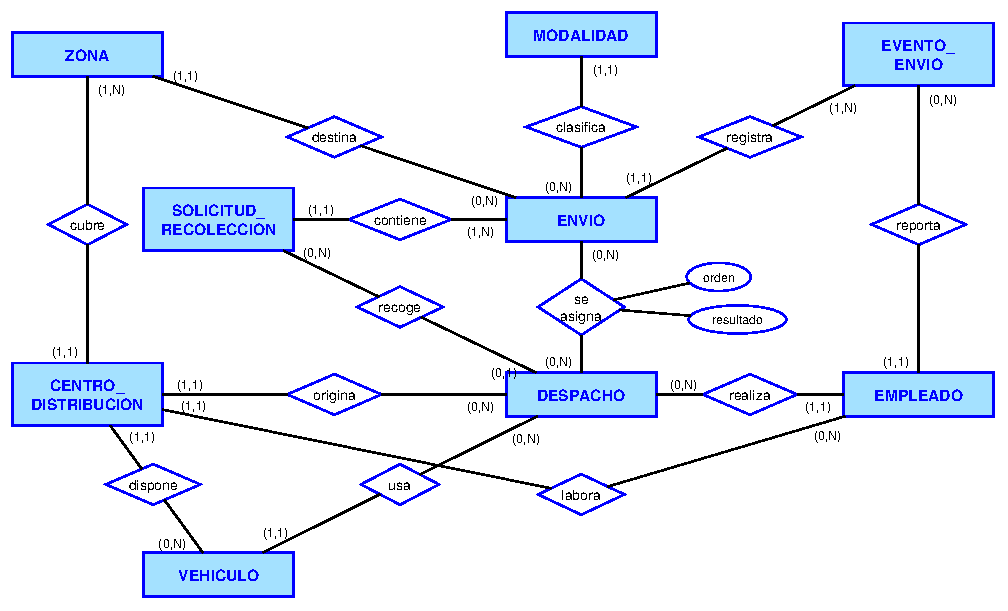
\includegraphics{figuras/er/M_U2.pdf}}
\caption{Vista U2 en el módulo: personal del centro de distribución.}
\label{fig:vistaU2}
\end{figure}
\par}

\textbf{U3 -- Mesa de servicio} (figura~\ref{fig:vistaU3}). Ve el envío
desde el cliente: quién lo pide, desde qué sede, a qué zona va, qué le
ha pasado y qué reclamaciones hay sobre él.

{\singlespacing
\begin{figure}[!htb]
\centering
\adjustbox{max width=\linewidth, max totalheight=0.42\textheight}{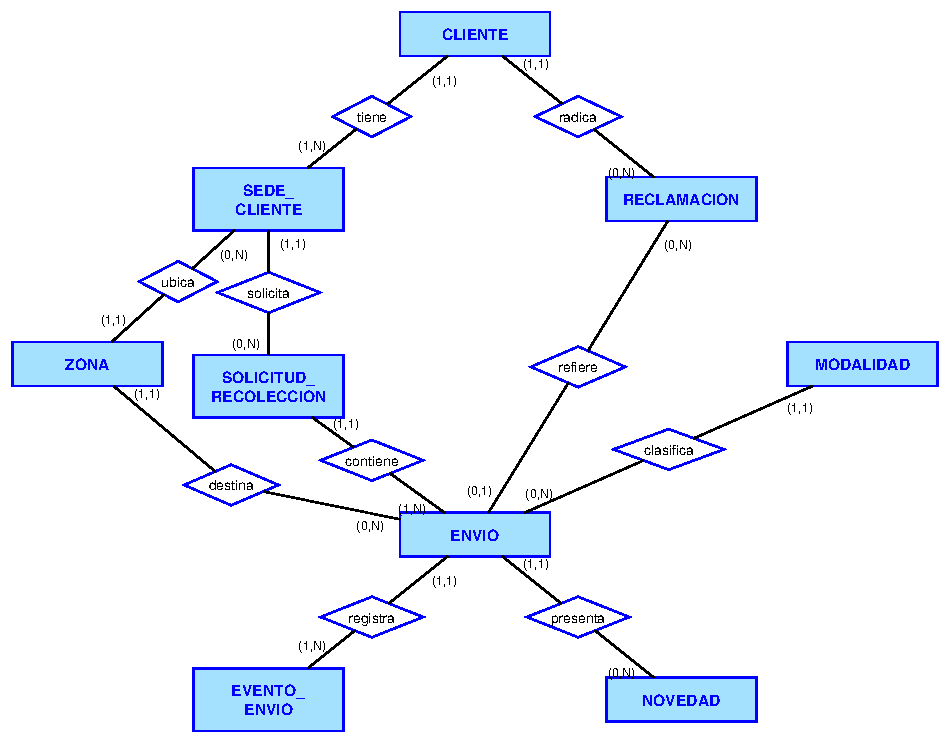
\includegraphics{figuras/er/M_U3.pdf}}
\caption{Vista U3 en el módulo: mesa de servicio.}
\label{fig:vistaU3}
\end{figure}
\par}

\textbf{U4 -- Mensajero} (figura~\ref{fig:vistaU4}). Trabaja con su
despacho del día: lo que recoge, lo que entrega y lo que registra en cada
visita (evento, prueba de entrega o novedad). Esta vista se presenta en
Data Modeler; allí la relación N:M entre ENVIO y DESPACHO
aparece como una entidad intermedia. Su versión en notación de Chen está
en la figura~\ref{fig:vistaU4chen} del anexo~\ref{anx:chen}.

{\singlespacing
\begin{figure}[!htb]
\centering
\adjustbox{max width=\linewidth, max totalheight=0.5\textheight}{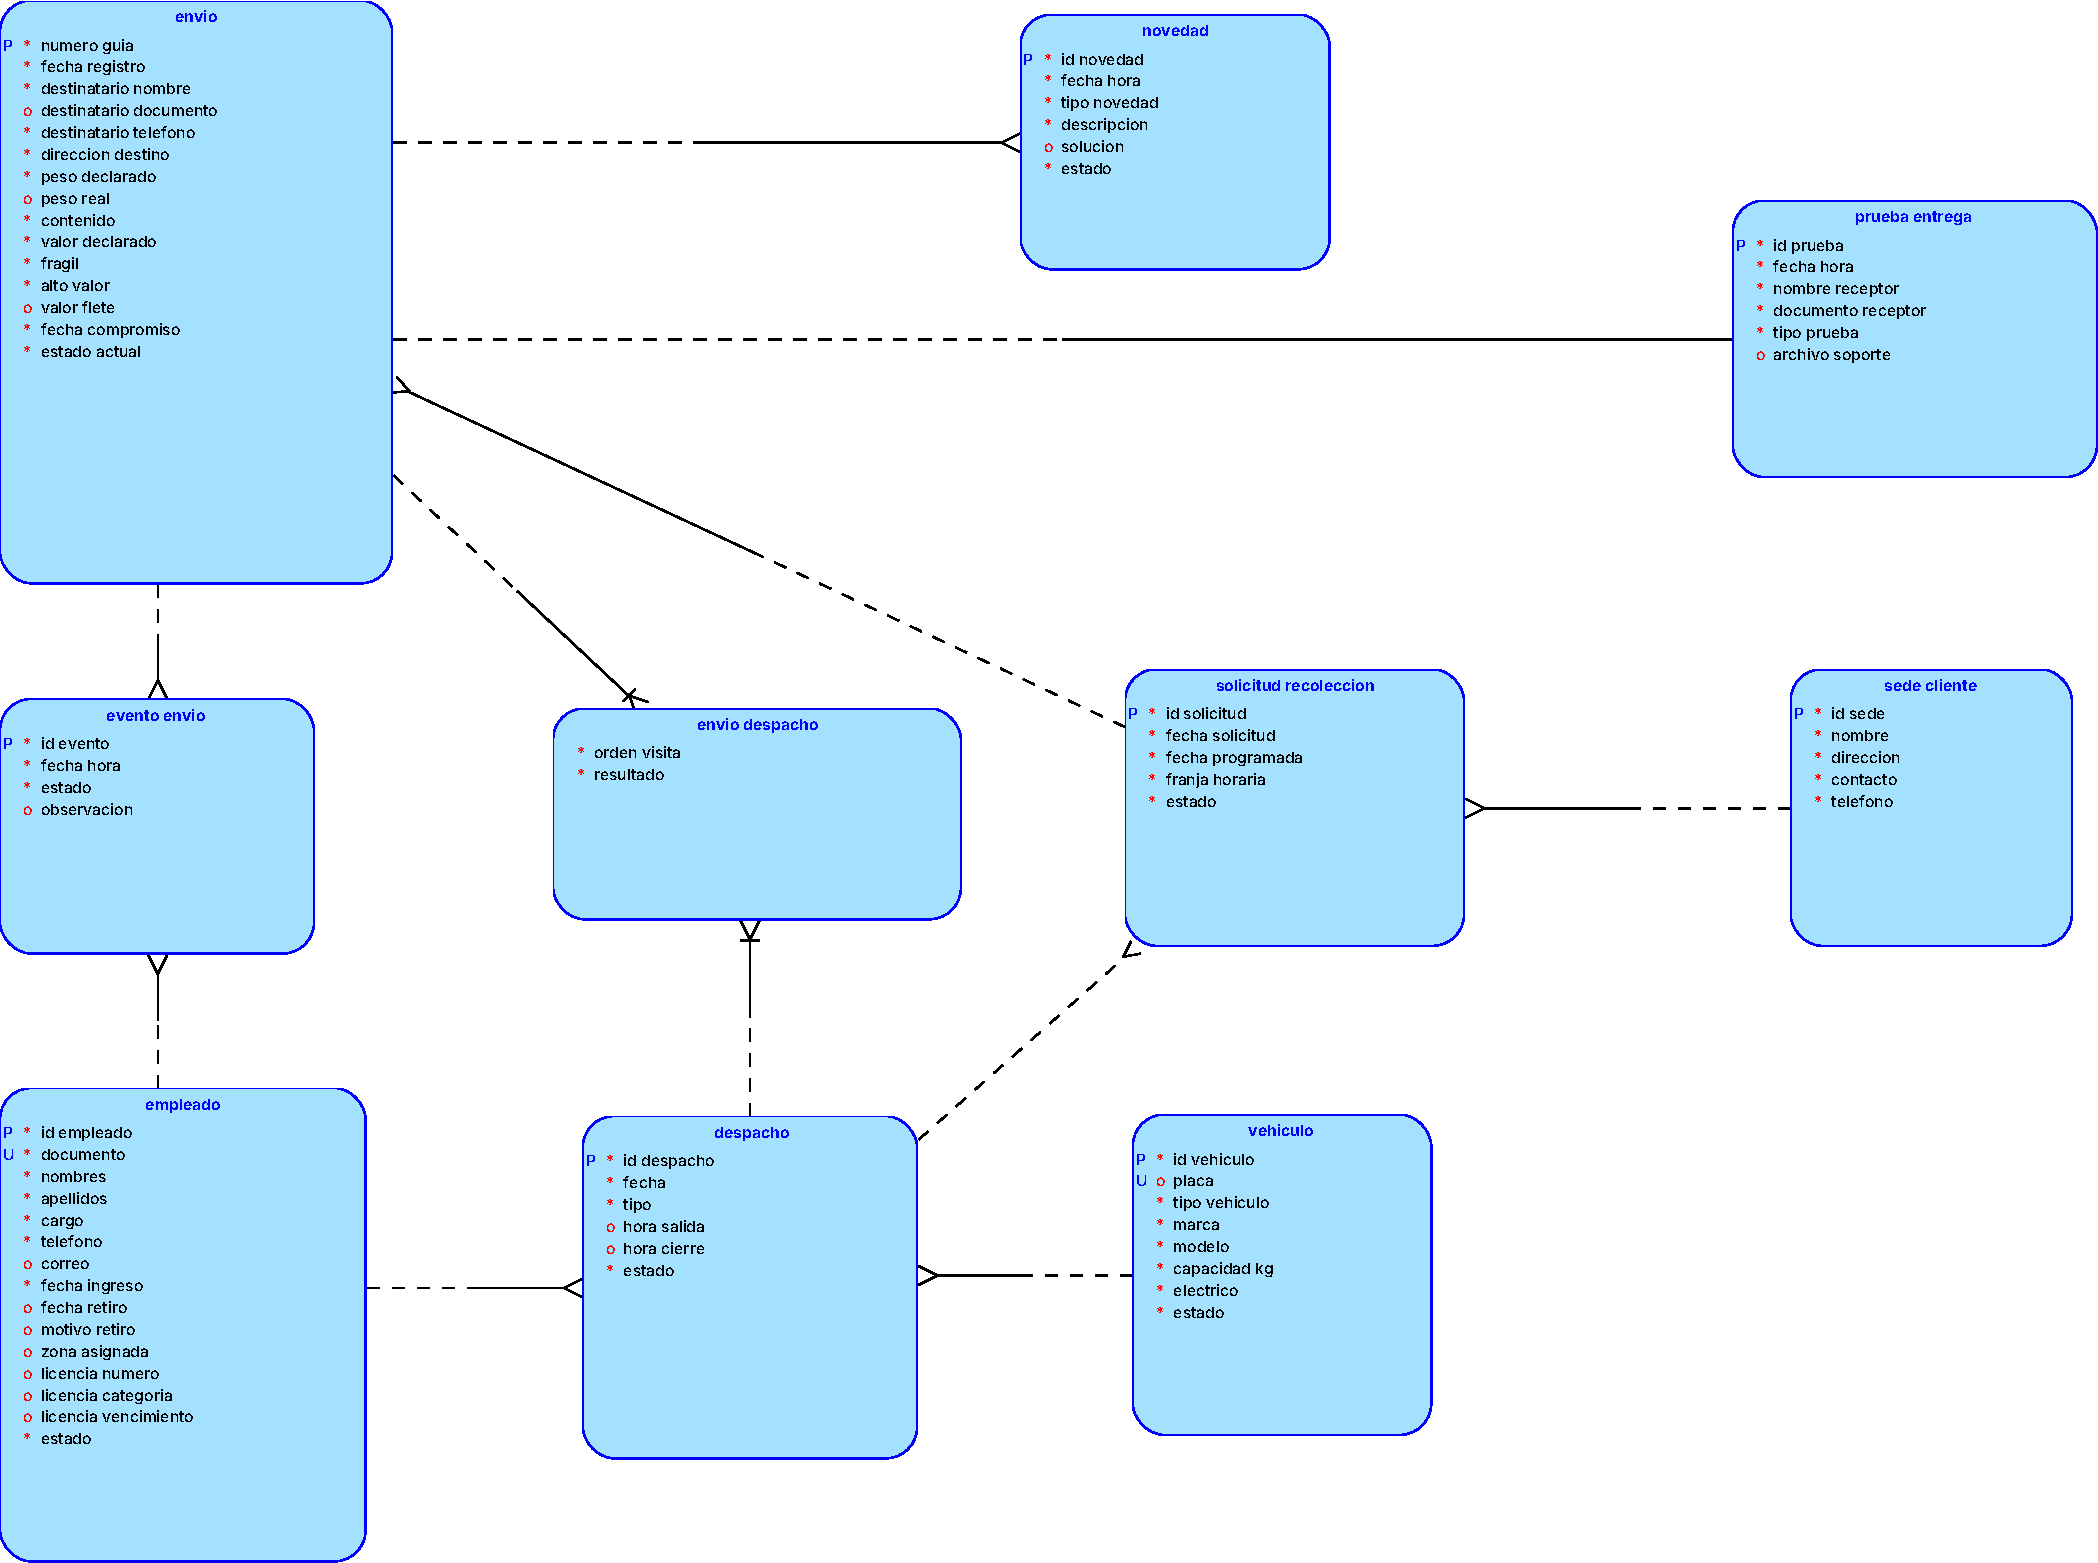
\includegraphics{figuras/datamodeler/dm_U4.pdf}}
\caption{Vista U4: mensajero, en Data Modeler (notación Barker).}
\label{fig:vistaU4}
\end{figure}
\par}

\subsubsection{Integración de Vistas (Prediseño Conceptual de la BD -- Modelo Entidad Relación)}
\label{sec:integracion}

Las vistas se integraron en cuatro pasos:

\begin{enumerate}[label=\arabic*.,leftmargin=1.2cm,itemsep=2pt]
  \item \textbf{Entidades comunes.} Las que aparecen en varias vistas
        (ENVIO, DESPACHO, ZONA, SOLICITUD\_RECOLECCION) representan lo
        mismo y quedan una sola vez; cuando una relación aparece en
        varias vistas se toma la participación más restrictiva.
  \item \textbf{Conflictos de nombre.} \textit{Guía} y \textit{paquete}
        se unifican en ENVIO; \textit{ruta} y \textit{planilla} en
        DESPACHO; \textit{conductor} y \textit{mensajero} en EMPLEADO;
        \textit{punto de recolección} en SEDE\_CLIENTE; \textit{rastreo}
        en EVENTO\_ENVIO.
  \item \textbf{Conflictos de estructura.} El estado del envío es
        atributo para la mesa de servicio y entidad (EVENTO\_ENVIO) para
        el centro; la zona fija del mensajero es atributo de EMPLEADO. El
        prediseño los deja así a propósito, como los describen los
        usuarios, y los corrige en la sección~\ref{sec:ajustes}.
  \item \textbf{Relaciones redundantes.} En el modelo global se eliminó
        la relación CLIENTE--\textit{envía}--ENVIO de la vista U7, que se
        obtiene por la sede y la solicitud (anexo~\ref{anx:global}). Entre
        las vistas del módulo no hay redundancias.
\end{enumerate}

El resultado es el prediseño del módulo (figura~\ref{fig:erintegrado}),
con 14 entidades y las 20 relaciones de la tabla~\ref{tab:relaciones}.
Es el subconjunto del prediseño global (figura~\ref{fig:erintegradoglobal})
formado por las entidades del módulo. Para compararlo con el resultado final, la
figura~\ref{fig:dmlogico} muestra a continuación el modelo del módulo
después de los ajustes de la sección~\ref{sec:ajustes}, construido en
Oracle SQL Developer Data Modeler.

\begin{landscape}
{\singlespacing
\begin{figure}[p]
\centering
\adjustbox{max width=22.5cm, max totalheight=14.6cm}{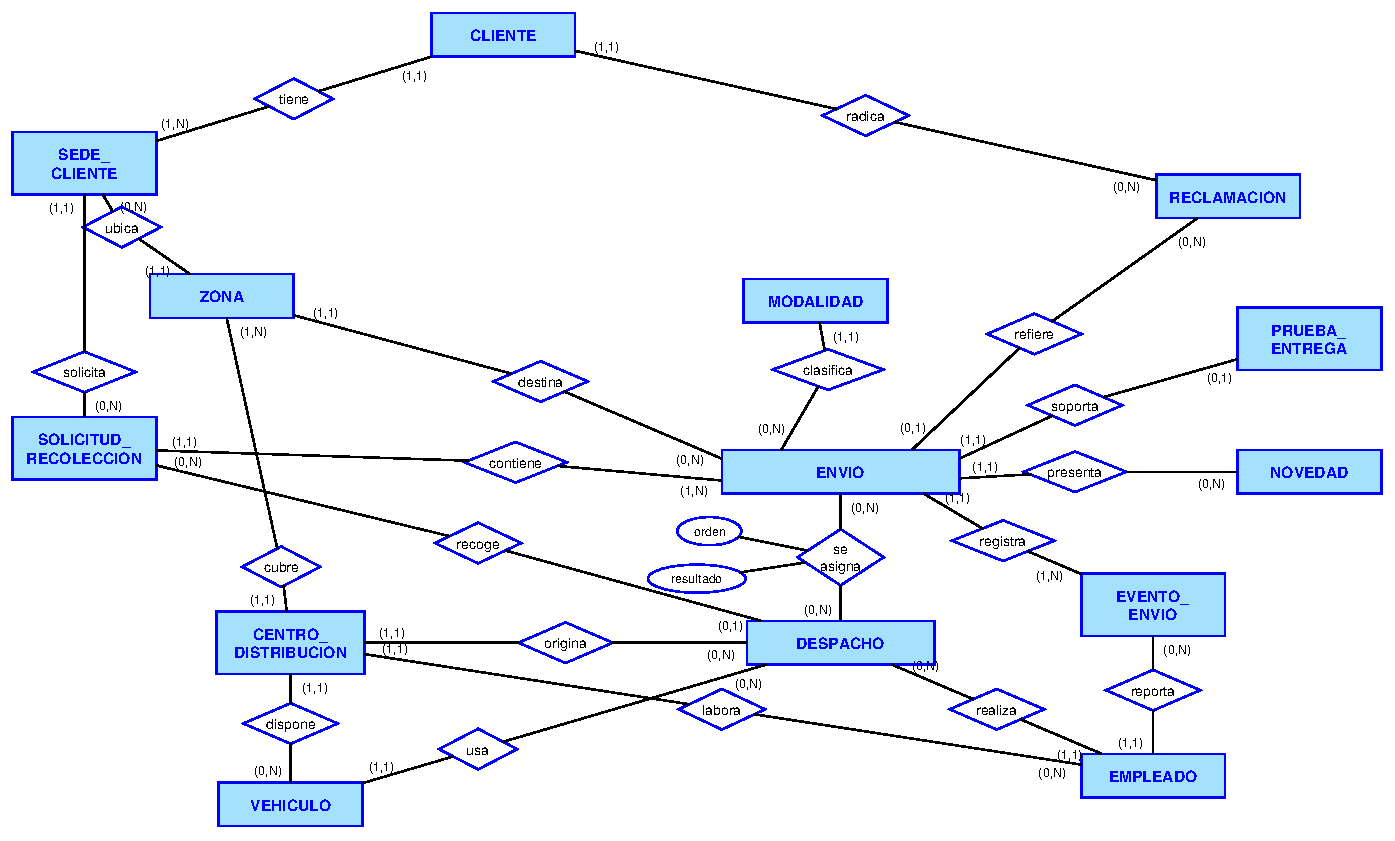
\includegraphics{figuras/er/M_prediseno.pdf}}
\caption{Prediseño conceptual del módulo de operación de envíos.}
\label{fig:erintegrado}
\end{figure}
\par}
\end{landscape}
\begin{landscape}
{\singlespacing
\begin{figure}[p]
\centering
\adjustbox{max width=22.5cm, max totalheight=14.6cm}{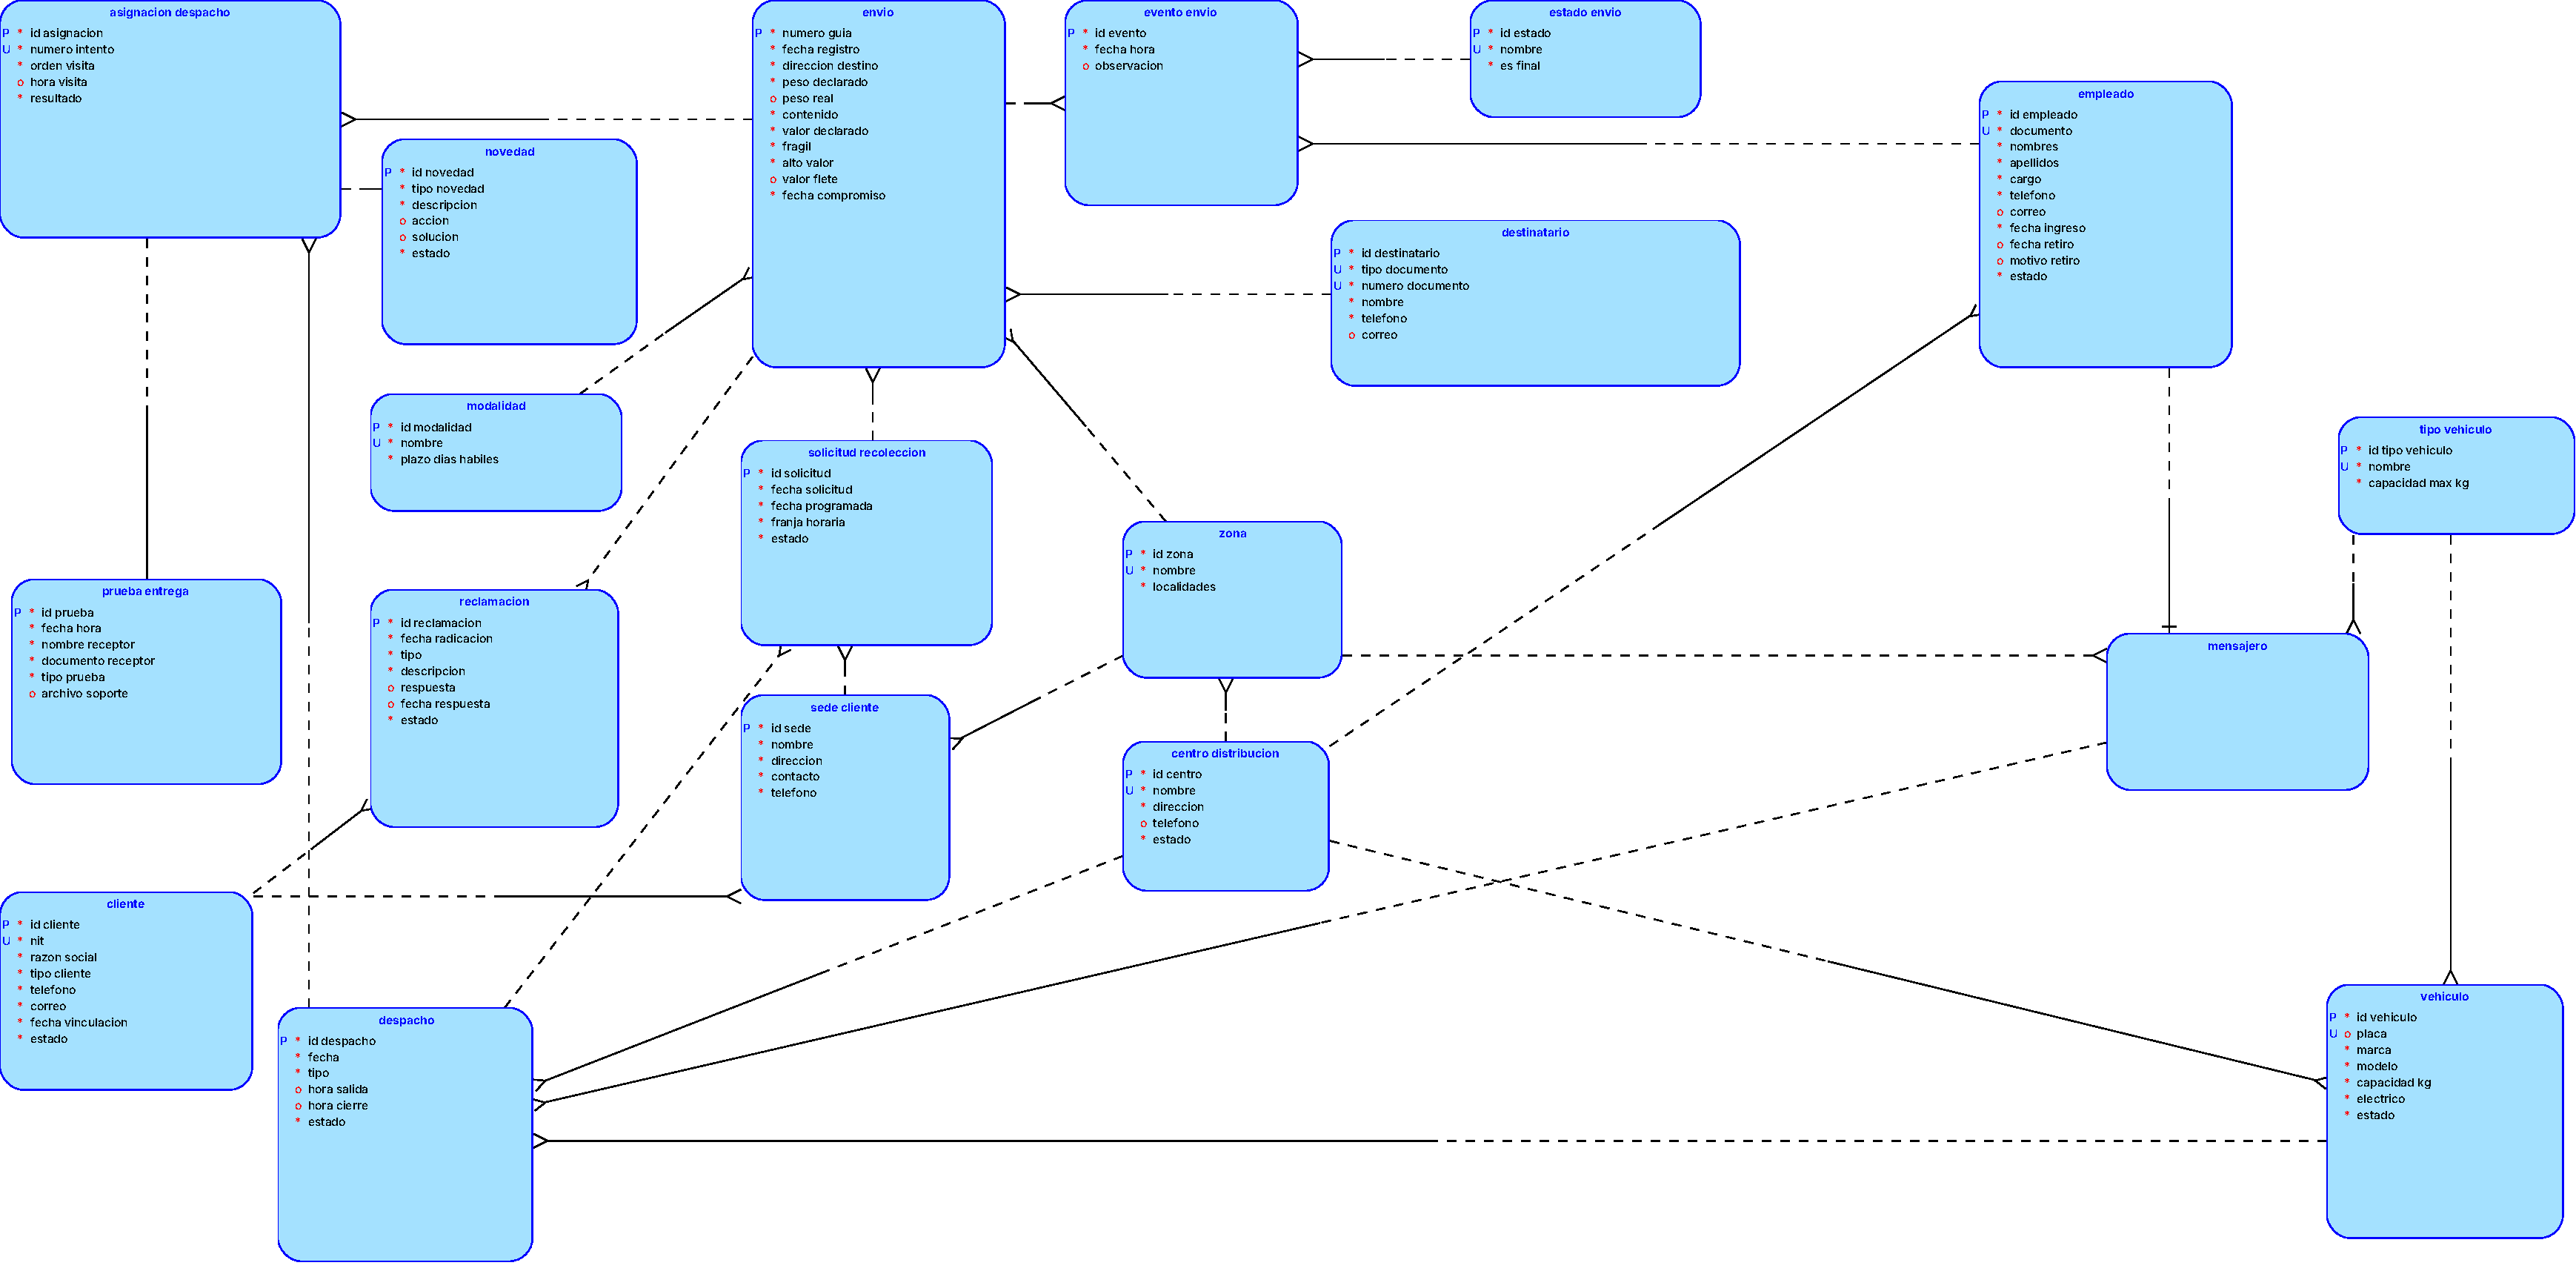
\includegraphics{figuras/datamodeler/dm_M_logico.pdf}}
\caption{Modelo Entidad-Relación ajustado del módulo de operación de envíos (resultado de los ajustes de la sección~\ref{sec:ajustes}), en Data Modeler (notación Barker).}
\label{fig:dmlogico}
\end{figure}
\par}
\end{landscape}
{\singlespacing\small
\begin{longtable}{L{1.5cm} L{4.9cm} L{0.8cm} L{2.4cm} L{3.9cm}}
\caption{Relaciones del prediseño del módulo.}
\label{tab:relaciones}\\
\toprule
\textbf{Relación} & \textbf{Entidades} & \textbf{Tipo} & \textbf{(mín,máx)} & \textbf{Significado} \\
\midrule
\endfirsthead
\toprule
\textbf{Relación} & \textbf{Entidades} & \textbf{Tipo} & \textbf{(mín,máx)} & \textbf{Significado} \\
\midrule
\endhead
\bottomrule
\endfoot
\textit{cubre} & CENTRO\_DISTRIBUCION --\allowbreak\ ZONA & 1:N & (1,1) -- (1,N) & Cada zona es atendida por un solo centro. \\
\textit{labora} & CENTRO\_DISTRIBUCION --\allowbreak\ EMPLEADO & 1:N & (1,1) -- (0,N) & Cada empleado trabaja en un centro. \\
\textit{dispone} & CENTRO\_DISTRIBUCION --\allowbreak\ VEHICULO & 1:N & (1,1) -- (0,N) & Cada vehículo está asignado a un centro. \\
\textit{origina} & CENTRO\_DISTRIBUCION --\allowbreak\ DESPACHO & 1:N & (1,1) -- (0,N) & Cada despacho sale de un centro. \\
\textit{ubica} & ZONA --\allowbreak\ SEDE\_CLIENTE & 1:N & (1,1) -- (0,N) & Cada sede del cliente está en una zona. \\
\textit{destina} & ZONA --\allowbreak\ ENVIO & 1:N & (1,1) -- (0,N) & Zona a la que va cada envío. \\
\textit{tiene} & CLIENTE --\allowbreak\ SEDE\_CLIENTE & 1:N & (1,1) -- (1,N) & Sedes de recolección de cada cliente. \\
\textit{clasifica} & MODALIDAD --\allowbreak\ ENVIO & 1:N & (1,1) -- (0,N) & Modalidad contratada para cada envío. \\
\textit{solicita} & SEDE\_CLIENTE --\allowbreak\ SOLICITUD\_RECOLECCION & 1:N & (1,1) -- (0,N) & Solicitudes hechas desde cada sede. \\
\textit{contiene} & SOLICITUD\_RECOLECCION --\allowbreak\ ENVIO & 1:N & (1,1) -- (1,N) & Envíos que se recogen en cada solicitud. \\
\textit{recoge} & DESPACHO --\allowbreak\ SOLICITUD\_RECOLECCION & 1:N & (0,1) -- (0,N) & Despacho de recolección que atiende cada solicitud. \\
\textit{se asigna} & ENVIO --\allowbreak\ DESPACHO & N:M & (0,N) -- (0,N) & Un envío puede salir en varios despachos (reintentos) y un despacho lleva muchos envíos. Atributos: orden, resultado. \\
\textit{registra} & ENVIO --\allowbreak\ EVENTO\_ENVIO & 1:N & (1,1) -- (1,N) & Historial de estados de cada envío. \\
\textit{reporta} & EMPLEADO --\allowbreak\ EVENTO\_ENVIO & 1:N & (1,1) -- (0,N) & Empleado responsable de cada evento. \\
\textit{soporta} & ENVIO --\allowbreak\ PRUEBA\_ENTREGA & 1:1 & (1,1) -- (0,1) & Constancia de recibo de cada envío. \\
\textit{presenta} & ENVIO --\allowbreak\ NOVEDAD & 1:N & (1,1) -- (0,N) & Novedades ocurridas con cada envío. \\
\textit{radica} & CLIENTE --\allowbreak\ RECLAMACION & 1:N & (1,1) -- (0,N) & Reclamaciones hechas por cada cliente. \\
\textit{refiere} & ENVIO --\allowbreak\ RECLAMACION & 1:N & (0,1) -- (0,N) & Envío sobre el que trata una reclamación (opcional). \\
\textit{usa} & VEHICULO --\allowbreak\ DESPACHO & 1:N & (1,1) -- (0,N) & Vehículo con el que se hace cada despacho. \\
\textit{realiza} & EMPLEADO --\allowbreak\ DESPACHO & 1:N & (1,1) -- (0,N) & Empleado (mensajero) que hace cada despacho. \\
\end{longtable}
\par}

%-----------------------------------------------------------------------
\subsection{Determinación de requerimientos de procesamiento}

Los requerimientos de procesamiento indican qué entra a la base de
datos, qué se hace con ello y qué se obtiene; de aquí salen las vistas,
consultas y procedimientos de los capítulos 4 a 6.

\subsubsection{Determinación de entradas, procesos y salidas por usuario}
\label{sec:eps}

La tabla~\ref{tab:eps} presenta los usuarios del módulo; los de los
demás módulos están en el anexo~\ref{anx:analisis}
(tabla~\ref{tab:epsotros}).

{\singlespacing\small
\begin{longtable}{L{1.9cm} L{3.9cm} L{4.6cm} L{3.9cm}}
\caption{Entradas, procesos y salidas de los usuarios del módulo.}
\label{tab:eps}\\
\toprule
\textbf{Usuario} & \textbf{Entradas} & \textbf{Procesos} & \textbf{Salidas} \\
\midrule
\endfirsthead
\toprule
\textbf{Usuario} & \textbf{Entradas} & \textbf{Procesos} & \textbf{Salidas} \\
\midrule
\endhead
\bottomrule
\endfoot
U1 Gerente general &
Periodo, centro o zona a consultar. &
Calcular el porcentaje de entregas a tiempo, el de envíos con novedad y
el tiempo de respuesta a reclamaciones. (Los indicadores de facturas,
rotación y flota se agregan con los demás módulos.) &
Indicadores de operación frente a las metas de la
tabla~\ref{tab:metas}. \\
\midrule
U2 Personal del centro &
Centros y zonas; programación de recolecciones; peso real de cada
paquete; valor del flete; envíos, mensajero y vehículo de cada despacho;
hora de salida y de cierre. &
Validar que el vehículo esté disponible y el mensajero activo antes de
crear el despacho (la validación de documentos, licencia y capacitación
se completa con M3 y M4); registrar eventos \textit{Recolectado},
\textit{En centro}, \textit{Clasificado} y \textit{En ruta}. &
Planilla de despacho; envíos pendientes por zona y modalidad; envíos que
vencen hoy; resultado del cierre de ruta. \\
\midrule
U3 Mesa de servicio &
Solicitudes de recolección; datos de los envíos y destinatarios;
decisiones sobre novedades; reclamaciones y sus respuestas. &
Verificar que el cliente esté activo (el contrato vigente se valida con
M2); generar el número de guía; controlar el número de intentos de
entrega; calcular el tiempo de respuesta de cada reclamación. &
Guía del envío; recorrido de un envío; novedades abiertas; reclamaciones
pendientes. \\
\midrule
U4 Mensajero &
Confirmación de recolección; prueba de entrega (firma, documento o
fotografía); novedad con su tipo. &
Registrar el evento con la fecha, la hora y el mensajero; impedir marcar
como entregado un envío sin prueba; impedir entregar a terceros los
envíos frágiles o de alto valor. &
Lista de su despacho con el orden de visita; datos de contacto del
destinatario. \\
\midrule
U9 Cliente &
Número de guía. &
Verificar que la guía pertenezca al cliente que consulta. &
Estado actual y recorrido del envío. \\
\end{longtable}
\par}

%-----------------------------------------------------------------------
\subsection{Ajustes al Diseño Conceptual de la BD -- Modelo Entidad Relación}
\label{sec:ajustes}

Al revisar el prediseño contra los requerimientos de procesamiento se
hicieron los ajustes de la tabla~\ref{tab:ajustes}. Los ajustes 1 a 5
se aplicaron al modelo global (anexo~\ref{anx:global}); el 6 es propio
del módulo.

{\singlespacing\small
\begin{longtable}{L{0.8cm} L{3.9cm} L{4.6cm} L{5.1cm}}
\caption{Ajustes realizados al prediseño conceptual.}
\label{tab:ajustes}\\
\toprule
\textbf{N.º} & \textbf{En el prediseño} & \textbf{Ajuste} & \textbf{Justificación} \\
\midrule
\endfirsthead
\toprule
\textbf{N.º} & \textbf{En el prediseño} & \textbf{Ajuste} & \textbf{Justificación} \\
\midrule
\endhead
\bottomrule
\endfoot
1 &
Los datos del destinatario (nombre, documento, teléfono) son atributos
de ENVIO. &
Se crea la entidad DESTINATARIO, relacionada con ENVIO mediante
\textit{dirigido} (1:N). La dirección de entrega y la zona se mantienen
en ENVIO. &
Las droguerías y tiendas envían con frecuencia a las mismas personas, lo
que repetía sus datos en cada envío. Además, la Ley 1581 exige poder
consultar, corregir o suprimir los datos de una persona, lo que es más
sencillo si están en un solo registro. La dirección se deja en el envío
porque puede cambiar de un envío a otro. \\
\midrule
2 &
La relación ENVIO--\textit{se asigna}--DESPACHO es N:M, con los
atributos orden y resultado. PRUEBA\_ENTREGA y NOVEDAD se relacionan
directamente con ENVIO. &
La relación se convierte en la entidad ASIGNACION\_DESPACHO, que
representa cada intento de entrega o recolección de un envío en un
despacho. PRUEBA\_ENTREGA y NOVEDAD pasan a relacionarse con ella
(1:1). &
Un envío puede salir en varios despachos (reintentos y devolución) y
cada intento termina en una entrega o en una novedad. Con el cambio se
sabe en qué intento, con qué mensajero y en qué despacho ocurrió cada
novedad, y se puede controlar el máximo de dos intentos. \\
\midrule
3 &
EMPLEADO tiene como atributos la zona asignada y los datos de la
licencia, aunque solo aplican a los mensajeros. EMPLEADO realiza
DESPACHO. &
Se crea MENSAJERO como especialización de EMPLEADO. La zona pasa a ser
la relación ZONA--\textit{atiende}--MENSAJERO, la licencia pasa a la
entidad LICENCIA\_CONDUCCION (1:N) y el despacho lo realiza un
MENSAJERO. En el módulo no se incluye LICENCIA\_CONDUCCION, que
pertenece a M4. &
Evita atributos vacíos para el resto de empleados, garantiza que solo un
mensajero pueda recibir un despacho y conserva el historial de licencias
(renovaciones y categorías), necesario para validar la vigencia en la
fecha del despacho. \\
\midrule
4 &
EVENTO\_ENVIO tiene el estado como texto libre y ENVIO guarda además el
estado actual. &
Se crea el catálogo ESTADO\_ENVIO, relacionado con EVENTO\_ENVIO
(\textit{indica}, 1:N). El estado actual se retira de ENVIO porque se
obtiene del último evento. &
Los indicadores y las reglas dependen de estados escritos siempre igual.
Guardar el estado en dos lugares permite que se contradigan; si en el
diseño físico se requiere por rendimiento, se agregará como dato
derivado controlado por la base de datos. \\
\midrule
5 &
El tipo de vehículo y el tipo de documento son atributos de texto de
VEHICULO y DOCUMENTO\_VEHICULO. &
Se crean los catálogos TIPO\_VEHICULO y TIPO\_DOCUMENTO, con la relación
\textit{exige} (N:M) entre ellos. El módulo solo incorpora
TIPO\_VEHICULO, porque VEHICULO lo referencia; lo demás es de M3. &
La política de seguridad vial exige que ningún documento
\textit{obligatorio} esté vencido. Con solo las fechas no se detecta un
documento que nunca se registró; con \textit{exige} se sabe qué
documentos debe tener cada tipo de vehículo (por ejemplo, la bicicleta
eléctrica no requiere SOAT). \\
\midrule
6 &
MENSAJERO guarda como texto el tipo de vehículo que puede conducir. &
Se reemplaza por la relación TIPO\_VEHICULO--\textit{conduce}--MENSAJERO
(1:N). Aplica solo al módulo. &
Evita escribir el mismo tipo de varias formas y permite verificar que
el vehículo de un despacho sea del tipo que conduce su mensajero. \\
\end{longtable}
\par}

El modelo ajustado del módulo tiene 19 entidades y 26 relaciones, más
la especialización parcial de EMPLEADO en MENSAJERO (no todos los
empleados son mensajeros). Se presenta en la figura~\ref{fig:dmlogico},
a continuación del prediseño; el diagrama en notación de Chen, con el
nombre de cada relación y su participación (mín,máx), está en la
figura~\ref{fig:erfinal} del anexo~\ref{anx:chen}. Ambos diagramas se
verificaron relación por relación; el de Data Modeler muestra 27
relaciones y no 26 porque la especialización EMPLEADO--MENSAJERO aparece
como una relación 1:1 identificadora. Respecto al
prediseño, se agregan DESTINATARIO, ASIGNACION\_DESPACHO, ESTADO\_ENVIO,
MENSAJERO y TIPO\_VEHICULO, y la relación N:M \textit{se asigna} se
reemplaza por ASIGNACION\_DESPACHO. Sus atributos se definen en el
diccionario de datos (sección~\ref{sec:diccionario}). Este modelo es la
entrada del diseño lógico.


\newpage

%======================================================================
%  Capitulo 4 - Diseno logico de bases de datos
%======================================================================

\section{Diseño lógico de bases de datos}

El diseño lógico transforma el modelo conceptual ajustado del módulo de
operación de envíos (figura~\ref{fig:dmlogico}; en notación de Chen,
figura~\ref{fig:erfinal}) en un modelo relacional:
tablas, columnas, claves primarias y claves foráneas, con sus reglas de
integridad. El resultado tiene 19 tablas, 130 columnas y 27 claves
foráneas.

%-----------------------------------------------------------------------
\subsection{Conversión del diseño conceptual al diseño lógico}

\subsubsection{Modelo Entidad Relación a Modelo Relacional}

La conversión aplica las tres reglas básicas del curso y dos reglas
complementarias para los casos que el modelo del módulo incluye:

\begin{enumerate}[label=\textbf{R\arabic*.},leftmargin=1.2cm,itemsep=2pt]
  \item \textbf{Toda entidad se convierte en tabla}, y su identificador
        en clave primaria. Las 19 entidades dan 19 tablas.
  \item \textbf{Toda relación 1:N se convierte en una propagación de
        clave}: la clave primaria del lado ``uno'' pasa como clave
        foránea a la tabla del lado ``muchos''. Si el mínimo del lado
        ``uno'' es 0, la clave foránea admite nulos.
  \item \textbf{Toda relación N:M se convierte en una tabla intermedia.}
        El módulo no tiene relaciones N:M: la única del prediseño
        (\textit{se asigna}) ya se convirtió en la entidad
        ASIGNACION\_DESPACHO en el ajuste 2.
  \item \textbf{Una relación 1:1 se convierte en una clave foránea única}
        en la tabla de participación opcional (PRUEBA\_ENTREGA y
        NOVEDAD respecto a ASIGNACION\_DESPACHO).
  \item \textbf{Una especialización se convierte en una tabla por
        subtipo}, cuya clave primaria es también clave foránea hacia la
        tabla del supertipo (MENSAJERO respecto a EMPLEADO).
\end{enumerate}

La tabla~\ref{tab:conversion} muestra cómo se convirtió cada relación.

{\singlespacing\small
\begin{longtable}{L{2.0cm} L{1.0cm} L{4.9cm} L{4.6cm} L{1.0cm}}
\caption{Conversión de las relaciones del modelo ER del módulo.}
\label{tab:conversion}\\
\toprule
\textbf{Relación} & \textbf{Regla} & \textbf{Entidades (lado uno -- lado muchos)} & \textbf{Clave foránea resultante} & \textbf{Nulo} \\
\midrule
\endfirsthead
\toprule
\textbf{Relación} & \textbf{Regla} & \textbf{Entidades (lado uno -- lado muchos)} & \textbf{Clave foránea resultante} & \textbf{Nulo} \\
\midrule
\endhead
\bottomrule
\endfoot
\textit{cubre} & R2 & CENTRO\_DISTRIBUCION -- ZONA & zona.id\_centro & No \\
\textit{labora} & R2 & CENTRO\_DISTRIBUCION -- EMPLEADO & empleado.id\_centro & No \\
\textit{dispone} & R2 & CENTRO\_DISTRIBUCION -- VEHICULO & vehiculo.id\_centro & No \\
\textit{origina} & R2 & CENTRO\_DISTRIBUCION -- DESPACHO & despacho.id\_centro & No \\
\textit{ubica} & R2 & ZONA -- SEDE\_CLIENTE & sede\_cliente.id\_zona & No \\
\textit{destina} & R2 & ZONA -- ENVIO & envio.id\_zona & No \\
\textit{atiende} & R2 & ZONA -- MENSAJERO & mensajero.id\_zona & Sí \\
\textit{tiene} & R2 & CLIENTE -- SEDE\_CLIENTE & sede\_cliente.id\_cliente & No \\
\textit{radica} & R2 & CLIENTE -- RECLAMACION & reclamacion.id\_cliente & No \\
\textit{clasifica} & R2 & MODALIDAD -- ENVIO & envio.id\_modalidad & No \\
\textit{solicita} & R2 & SEDE\_CLIENTE -- SOLICITUD\_RECOLECCION & solicitud\_recoleccion.id\_sede & No \\
\textit{contiene} & R2 & SOLICITUD\_RECOLECCION -- ENVIO & envio.id\_solicitud & No \\
\textit{recoge} & R2 & DESPACHO -- SOLICITUD\_RECOLECCION & solicitud\_recoleccion.id\_despacho & Sí \\
\textit{dirigido} & R2 & DESTINATARIO -- ENVIO & envio.id\_destinatario & No \\
\textit{se asigna} & R2 & ENVIO -- ASIGNACION\_DESPACHO & asignacion\_despacho.numero\_guia & No \\
\textit{agrupa} & R2 & DESPACHO -- ASIGNACION\_DESPACHO & asignacion\_despacho.id\_despacho & No \\
\textit{soporta} & R4 & ASIGNACION\_DESPACHO -- PRUEBA\_ENTREGA & prueba\_entrega.id\_asignacion (única) & No \\
\textit{presenta} & R4 & ASIGNACION\_DESPACHO -- NOVEDAD & novedad.id\_asignacion (única) & No \\
\textit{registra} & R2 & ENVIO -- EVENTO\_ENVIO & evento\_envio.numero\_guia & No \\
\textit{indica} & R2 & ESTADO\_ENVIO -- EVENTO\_ENVIO & evento\_envio.id\_estado & No \\
\textit{reporta} & R2 & EMPLEADO -- EVENTO\_ENVIO & evento\_envio.id\_empleado & No \\
\textit{refiere} & R2 & ENVIO -- RECLAMACION & reclamacion.numero\_guia & Sí \\
\textit{usa} & R2 & VEHICULO -- DESPACHO & despacho.id\_vehiculo & No \\
\textit{realiza} & R2 & MENSAJERO -- DESPACHO & despacho.id\_mensajero & No \\
\textit{categoriza} & R2 & TIPO\_VEHICULO -- VEHICULO & vehiculo.id\_tipo\_vehiculo & No \\
\textit{conduce} & R2 & TIPO\_VEHICULO -- MENSAJERO & mensajero.id\_tipo\_vehiculo & No \\
\textit{es un} & R5 & EMPLEADO -- MENSAJERO & mensajero.id\_empleado (PK y FK) & No \\
\end{longtable}
\par}

Las claves foráneas que admiten nulos son exactamente las de las
relaciones con mínimo 0 en el lado ``uno'' (\textit{atiende},
\textit{recoge} y \textit{refiere}); las demás son obligatorias.

\subsubsection{Reglas de Integridad (Propias del Modelo relacional y propias del desarrollador)}

\textbf{Reglas propias del modelo relacional.} Se garantizan con la
estructura de las tablas (tabla~\ref{tab:integridad}).

{\singlespacing\small
\begin{longtable}{L{3.2cm} L{8.2cm} L{2.6cm}}
\caption{Reglas de integridad propias del modelo relacional.}
\label{tab:integridad}\\
\toprule
\textbf{Regla} & \textbf{Cómo se aplica en el módulo} & \textbf{Restricciones} \\
\midrule
\endfirsthead
\toprule
\textbf{Regla} & \textbf{Cómo se aplica en el módulo} & \textbf{Restricciones} \\
\midrule
\endhead
\bottomrule
\endfoot
Integridad de entidad & Cada tabla tiene clave primaria, única y no nula. Se usan claves sustitutas numéricas, salvo ENVIO, cuya clave es el número de guía. Las claves naturales (NIT, documento, placa, nombres de catálogos) se declaran únicas. & 19 PRIMARY KEY, 13 UNIQUE \\
\midrule
Integridad referencial & Toda clave foránea apunta a una fila existente. No se define borrado en cascada: la política de acceso prohíbe eliminar registros, que se anulan por estado, así que el motor rechaza borrar una fila referenciada. & 27 FOREIGN KEY \\
\midrule
Integridad de dominio & Cada columna tiene tipo y tamaño; las obligatorias son NOT NULL; los estados y tipos solo admiten los valores de su lista, y los estados iniciales tienen valor por defecto. & 110 NOT NULL, 33 CHECK, 12 DEFAULT \\
\end{longtable}
\par}

\textbf{Reglas propias del desarrollador.} Son las reglas de negocio
que salen de las políticas y de la caracterización de los procesos
(tabla~\ref{tab:reglasnegocio}). Las que se pueden expresar sobre una
sola fila o con unicidad ya están en el modelo lógico; las que
dependen de otras filas o tablas se implementarán con disparadores,
procedimientos y permisos en el diseño físico.

{\singlespacing\small
\begin{longtable}{L{1.0cm} L{6.6cm} L{2.6cm} L{4.2cm}}
\caption{Reglas de negocio del módulo.}
\label{tab:reglasnegocio}\\
\toprule
\textbf{Cód.} & \textbf{Regla} & \textbf{Origen} & \textbf{Implementación} \\
\midrule
\endfirsthead
\toprule
\textbf{Cód.} & \textbf{Regla} & \textbf{Origen} & \textbf{Implementación} \\
\midrule
\endhead
\bottomrule
\endfoot
RN01 & Cada envío tiene un número de guía único. & Calidad del servicio & PK de envio \\
RN02 & Todo envío se registra con destinatario, dirección, zona, modalidad, peso, contenido y fecha de compromiso. & Calidad del servicio & NOT NULL en envio \\
RN03 & La fecha de compromiso no es anterior a la de registro, los pesos y el flete son positivos y el valor declarado no es negativo. & P1 & CHECK envio\_compromiso\_ck, envio\_pesos\_ck, envio\_valor\_ck \\
RN04 & Un destinatario existe una sola vez (tipo y número de documento). & Datos personales & UNIQUE destinatario\_documento\_uk \\
RN05 & Ningún envío se marca como entregado sin prueba de entrega. & Calidad del servicio & Disparador (diseño físico) \\
RN06 & Los envíos frágiles o de alto valor solo se entregan al destinatario: el documento de quien recibe debe ser el del destinatario. & Manejo de la mercancía & Disparador (diseño físico) \\
RN07 & Máximo dos intentos de entrega; el tercero solo puede ser la devolución y solo después de dos novedades. & P3 & CHECK asignacion\_intento\_ck, UNIQUE asignacion\_intento\_uk y disparador \\
RN08 & Cada intento tiene como máximo una prueba de entrega o una novedad. & P2 & UNIQUE prueba\_asignacion\_uk, novedad\_asignacion\_uk \\
RN09 & Solo un mensajero puede realizar un despacho. & Seguridad vial & FK despacho\_mensajero\_fk \\
RN10 & Al crear un despacho, el vehículo debe estar DISPONIBLE y el mensajero ACTIVO (la validación de documentos, licencia y capacitación se agrega con M3 y M4). & Seguridad vial & Disparador (diseño físico) \\
RN11 & El vehículo del despacho debe ser del tipo que conduce el mensajero. & Seguridad vial & Disparador (diseño físico) \\
RN12 & Todo envío nace con el evento REGISTRADO y sus estados siguen el ciclo de vida (no se pasa a ENTREGADO sin haber estado EN\_RUTA). & Seguimiento por eventos & Procedimiento de registro y disparador \\
RN13 & Cada evento registra el empleado responsable. & Manejo de la mercancía & FK NOT NULL evento\_empleado\_fk \\
RN14 & La respuesta a una reclamación es posterior a su radicación; la meta de cuatro horas se mide como indicador. & OE2 & CHECK reclamacion\_resp\_ck y vista \\
RN15 & Solo se registran solicitudes de clientes activos (hasta integrar los contratos de M2). & P1 & Disparador (diseño físico) \\
RN16 & No se eliminan registros; se anulan o cierran por estado. & Acceso a la información & Permisos sin DELETE (diseño físico) \\
\end{longtable}
\par}

\subsubsection{Optimización del Diseño Lógico de la BD}

Antes de normalizar se tomaron las siguientes decisiones de diseño:

\begin{enumerate}[label=\arabic*.,leftmargin=1.2cm,itemsep=2pt]
  \item \textbf{Claves.} El número de guía es la clave de ENVIO porque
        es estable, va impreso en el paquete y es lo que el cliente
        consulta. Las demás tablas usan claves sustitutas numéricas, más
        cortas y estables que las naturales, que se conservan como
        únicas.
  \item \textbf{Estado actual del envío.} No se guarda en ENVIO, porque
        se deduce del último evento y guardarlo dos veces permitiría
        contradicciones (ajuste 4). Se obtiene con la vista
        v\_estado\_actual\_envio; si en el diseño físico se necesita por
        rendimiento, se agregará como dato derivado mantenido por un
        disparador.
  \item \textbf{Prueba y novedad en tablas propias.} Podrían ser columnas
        de ASIGNACION\_DESPACHO, pero cada intento tiene una u otra, nunca
        las dos, y la mayoría de columnas quedaría nula. Separarlas con
        una clave foránea única evita los nulos y permite reglas propias
        para cada una.
  \item \textbf{Mensajero como tabla de subtipo.} Guardar la zona y el
        tipo de vehículo en EMPLEADO dejaría esas columnas vacías para
        quien no es mensajero, y no impediría asignar un despacho a otro
        cargo. La tabla MENSAJERO resuelve ambas cosas.
  \item \textbf{Catálogos frente a listas fijas.} Son tablas los
        dominios que tienen atributos propios o que usan las reglas
        (estados del envío, modalidades, tipos de vehículo); son listas
        CHECK los dominios simples que no cambian (franja horaria, tipo
        de prueba, tipo de novedad).
  \item \textbf{Resultado del intento.} El dominio de
        asignacion\_despacho.resultado queda en PENDIENTE, ENTREGADO,
        NOVEDAD y DEVUELTO, y el número de intento entre 1 y 3: los dos
        primeros son de entrega y el tercero es la devolución.
  \item \textbf{Integración futura.} Las columnas que dependen de otros
        módulos (envio.id\_factura, reclamacion.id\_factura) no se crean
        todavía; al integrar M2 se agregan sin modificar las columnas
        existentes.
\end{enumerate}

\subsubsection{Normalización y Formas Normales}

La normalización detecta y elimina redundancias que causan anomalías de
inserción, actualización y borrado. Una tabla está en primera forma
normal (1FN) si todos sus valores son atómicos; en segunda (2FN) si
está en 1FN y cada atributo no clave depende de la clave completa; en
tercera (3FN) si está en 2FN y ningún atributo no clave depende de otro
atributo no clave; y en forma normal de Boyce-Codd (FNBC) si todo
determinante es clave candidata.

Para comprobar el diseño se parte de cómo vería los datos alguien que
no ha modelado: una sola tabla con todo lo que se anota de una guía.

\begin{sloppypar}\noindent\textbf{Forma no normalizada.} GUIA(\pk{numero\_guia}, fecha\_registro,
nit\_cliente, razon\_social, direccion\_sede, zona\_sede,
documento\_destinatario, nombre\_destinatario, telefono\_destinatario,
direccion\_destino, zona\_destino, centro\_zona, modalidad,
plazo\_modalidad, peso\_declarado, peso\_real, contenido,
valor\_declarado, fragil, alto\_valor, valor\_flete, fecha\_compromiso,
\{fecha\_hora\_evento, estado, documento\_empleado, nombre\_empleado\},
\{id\_despacho, fecha\_despacho, placa, tipo\_vehiculo, capacidad\_tipo,
documento\_mensajero, nombre\_mensajero, orden\_visita, intento,
resultado, quien\_recibe, tipo\_prueba, tipo\_novedad,
descripcion\_novedad\}). Las llaves marcan grupos repetitivos: una guía
tiene varios eventos y varias visitas.\end{sloppypar}

\begin{sloppypar}\noindent\textbf{Primera forma normal.} Los grupos repetitivos salen a tablas
propias con la clave de la guía:
EVENTO(\pk{numero\_guia, fecha\_hora}, estado, documento\_empleado,
nombre\_empleado) y VISITA(\pk{numero\_guia, id\_despacho},
fecha\_despacho, placa, tipo\_vehiculo, capacidad\_tipo,
documento\_mensajero, nombre\_mensajero, orden\_visita, intento,
resultado, quien\_recibe, tipo\_prueba, tipo\_novedad,
descripcion\_novedad).\end{sloppypar}

\begin{sloppypar}\noindent\textbf{Segunda forma normal.} En VISITA, fecha\_despacho, placa,
tipo\_vehiculo, capacidad\_tipo y los datos del mensajero dependen solo
de id\_despacho, que es parte de la clave. Se separan en
DESPACHO(\pk{id\_despacho}, fecha, placa, tipo\_vehiculo,
capacidad\_tipo, documento\_mensajero, nombre\_mensajero). GUIA y
EVENTO ya cumplen 2FN: GUIA tiene clave simple y en EVENTO todos los
atributos dependen de la guía y del momento juntos.\end{sloppypar}

\textbf{Tercera forma normal.} Se eliminan las dependencias
transitivas:

\begin{itemize}[leftmargin=1.2cm,itemsep=1pt]
  \item En GUIA: documento\_destinatario $\rightarrow$ nombre, teléfono
        (sale DESTINATARIO); la guía pertenece a una solicitud, la
        solicitud a una sede y la sede a un cliente: sede $\rightarrow$
        cliente, dirección, zona y nit $\rightarrow$ razón social (salen
        SOLICITUD\_RECOLECCION, SEDE\_CLIENTE y CLIENTE); zona
        $\rightarrow$ centro (salen ZONA y CENTRO\_DISTRIBUCION);
        modalidad $\rightarrow$ plazo (sale MODALIDAD).
  \item En EVENTO: documento\_empleado $\rightarrow$ nombre (sale
        EMPLEADO) y estado $\rightarrow$ es\_final (sale ESTADO\_ENVIO).
  \item En DESPACHO: placa $\rightarrow$ tipo, marca, capacidad y tipo
        $\rightarrow$ capacidad máxima (salen VEHICULO y TIPO\_VEHICULO);
        documento\_mensajero $\rightarrow$ nombre (sale MENSAJERO, con
        sus datos de empleado en EMPLEADO).
  \item En VISITA no hay dependencias transitivas, pero los datos de
        prueba y de novedad son excluyentes y casi siempre nulos; por la
        decisión 3 de optimización salen a PRUEBA\_ENTREGA y NOVEDAD, y
        VISITA toma el nombre ASIGNACION\_DESPACHO con una clave
        sustituta.
\end{itemize}

\textbf{Forma normal de Boyce-Codd.} En las tablas resultantes todo
determinante es clave candidata (tabla~\ref{tab:formasnormales}). Las
únicas tablas con más de una clave candidata son DESTINATARIO, cuyo
documento también la identifica, y ASIGNACION\_DESPACHO, que también se
identifica por (guía, despacho) y por (guía, intento); ambas se declaran
únicas. El resultado coincide con las tablas obtenidas por conversión
del modelo ER, lo que confirma que el diseño conceptual era correcto.

{\singlespacing\small
\begin{longtable}{L{3.6cm} L{3.8cm} L{5.4cm} L{1.2cm}}
\caption{Dependencias funcionales y forma normal de cada tabla.}
\label{tab:formasnormales}\\
\toprule
\textbf{Tabla} & \textbf{Claves candidatas} & \textbf{Dependencias funcionales} & \textbf{FN} \\
\midrule
\endfirsthead
\toprule
\textbf{Tabla} & \textbf{Claves candidatas} & \textbf{Dependencias funcionales} & \textbf{FN} \\
\midrule
\endhead
\bottomrule
\endfoot
centro\_distribucion & id\_centro; nombre & id\_centro $\rightarrow$ resto; nombre $\rightarrow$ id\_centro & FNBC \\
zona & id\_zona; nombre & id\_zona $\rightarrow$ resto; nombre $\rightarrow$ id\_zona & FNBC \\
cliente & id\_cliente; nit & id\_cliente $\rightarrow$ resto; nit $\rightarrow$ id\_cliente & FNBC \\
sede\_cliente & id\_sede & id\_sede $\rightarrow$ resto & FNBC \\
modalidad & id\_modalidad; nombre & id\_modalidad $\rightarrow$ resto; nombre $\rightarrow$ id\_modalidad & FNBC \\
tipo\_vehiculo & id\_tipo\_vehiculo; nombre & id\_tipo\_vehiculo $\rightarrow$ resto; nombre $\rightarrow$ id\_tipo\_vehiculo & FNBC \\
vehiculo & id\_vehiculo; placa (si existe) & id\_vehiculo $\rightarrow$ resto; placa $\rightarrow$ id\_vehiculo & FNBC \\
empleado & id\_empleado; documento & id\_empleado $\rightarrow$ resto; documento $\rightarrow$ id\_empleado & FNBC \\
mensajero & id\_empleado & id\_empleado $\rightarrow$ id\_zona, id\_tipo\_vehiculo & FNBC \\
destinatario & id\_destinatario; (tipo\_documento, numero\_documento) & id\_destinatario $\rightarrow$ resto; documento $\rightarrow$ id\_destinatario & FNBC \\
despacho & id\_despacho & id\_despacho $\rightarrow$ resto & FNBC \\
solicitud\_recoleccion & id\_solicitud & id\_solicitud $\rightarrow$ resto & FNBC \\
envio & numero\_guia & numero\_guia $\rightarrow$ resto & FNBC \\
asignacion\_despacho & id\_asignacion; (numero\_guia, id\_despacho); (numero\_guia, numero\_intento) & cada clave $\rightarrow$ resto & FNBC \\
estado\_envio & id\_estado; nombre & id\_estado $\rightarrow$ resto; nombre $\rightarrow$ id\_estado & FNBC \\
evento\_envio & id\_evento & id\_evento $\rightarrow$ resto & FNBC \\
prueba\_entrega & id\_prueba; id\_asignacion & cada clave $\rightarrow$ resto & FNBC \\
novedad & id\_novedad; id\_asignacion & cada clave $\rightarrow$ resto & FNBC \\
reclamacion & id\_reclamacion & id\_reclamacion $\rightarrow$ resto & FNBC \\
\end{longtable}
\par}

\subsubsection{Diseño Lógico de la Base de Datos -- Modelo Relacional}
\label{sec:esquemarel}

La figura~\ref{fig:dmrelacional} presenta el modelo relacional del
módulo, construido en Data Modeler. En cada tabla,
\texttt{P} marca la clave primaria, \texttt{F} una clave foránea,
\texttt{U} un valor único y \texttt{*} una columna obligatoria; cada
línea entre tablas es una clave foránea. Tiene 19 tablas con sus 19 claves
primarias, las 13 restricciones de unicidad, las 27 claves foráneas con
sus nombres. Las vistas de usuario no se dibujan en el diagrama, porque no
tienen claves foráneas; se describen más adelante. Una versión elaborada en draw.io, que indica
junto a cada clave foránea la tabla a la que apunta, está en la
figura~\ref{fig:relacional} del anexo~\ref{anx:chen}.


En notación de esquema relacional (clave primaria subrayada, claves
foráneas en cursiva):

{\singlespacing\small\sloppy
\begin{itemize}[leftmargin=0.6cm,itemsep=3pt,label={}]
  \item \textbf{CENTRO\_DISTRIBUCION}(\pk{id\_centro}, nombre, direccion, telefono, estado)
  \item \textbf{ZONA}(\pk{id\_zona}, \fk{id\_centro}, nombre, localidades)
  \item \textbf{CLIENTE}(\pk{id\_cliente}, nit, razon\_social, tipo\_cliente, telefono, correo, fecha\_vinculacion, estado)
  \item \textbf{SEDE\_CLIENTE}(\pk{id\_sede}, \fk{id\_cliente}, \fk{id\_zona}, nombre, direccion, contacto, telefono)
  \item \textbf{MODALIDAD}(\pk{id\_modalidad}, nombre, plazo\_dias\_habiles)
  \item \textbf{TIPO\_VEHICULO}(\pk{id\_tipo\_vehiculo}, nombre, capacidad\_max\_kg)
  \item \textbf{VEHICULO}(\pk{id\_vehiculo}, \fk{id\_centro}, \fk{id\_tipo\_vehiculo}, placa, marca, modelo, capacidad\_kg, electrico, estado)
  \item \textbf{EMPLEADO}(\pk{id\_empleado}, \fk{id\_centro}, documento, nombres, apellidos, cargo, telefono, correo, fecha\_ingreso, fecha\_retiro, motivo\_retiro, estado)
  \item \textbf{MENSAJERO}(\pk{\fk{id\_empleado}}, \fk{id\_zona}, \fk{id\_tipo\_vehiculo})
  \item \textbf{DESTINATARIO}(\pk{id\_destinatario}, tipo\_documento, numero\_documento, nombre, telefono, correo)
  \item \textbf{DESPACHO}(\pk{id\_despacho}, \fk{id\_centro}, \fk{id\_vehiculo}, \fk{id\_mensajero}, fecha, tipo, hora\_salida, hora\_cierre, estado)
  \item \textbf{SOLICITUD\_RECOLECCION}(\pk{id\_solicitud}, \fk{id\_sede}, \fk{id\_despacho}, fecha\_solicitud, fecha\_programada, franja\_horaria, estado)
  \item \textbf{ENVIO}(\pk{numero\_guia}, \fk{id\_solicitud}, \fk{id\_destinatario}, \fk{id\_zona}, \fk{id\_modalidad}, fecha\_registro, direccion\_destino, peso\_declarado, peso\_real, contenido, valor\_declarado, fragil, alto\_valor, valor\_flete, fecha\_compromiso)
  \item \textbf{ASIGNACION\_DESPACHO}(\pk{id\_asignacion}, \fk{numero\_guia}, \fk{id\_despacho}, numero\_intento, orden\_visita, hora\_visita, resultado)
  \item \textbf{ESTADO\_ENVIO}(\pk{id\_estado}, nombre, es\_final)
  \item \textbf{EVENTO\_ENVIO}(\pk{id\_evento}, \fk{numero\_guia}, \fk{id\_estado}, \fk{id\_empleado}, fecha\_hora, observacion)
  \item \textbf{PRUEBA\_ENTREGA}(\pk{id\_prueba}, \fk{id\_asignacion}, fecha\_hora, nombre\_receptor, documento\_receptor, tipo\_prueba, archivo\_soporte)
  \item \textbf{NOVEDAD}(\pk{id\_novedad}, \fk{id\_asignacion}, tipo\_novedad, descripcion, accion, solucion, estado)
  \item \textbf{RECLAMACION}(\pk{id\_reclamacion}, \fk{id\_cliente}, \fk{numero\_guia}, fecha\_radicacion, tipo, descripcion, respuesta, fecha\_respuesta, estado)
\end{itemize}
\par}
\begin{landscape}
{\singlespacing
\begin{figure}[p]
\centering
\adjustbox{max width=22.5cm, max totalheight=14.6cm}{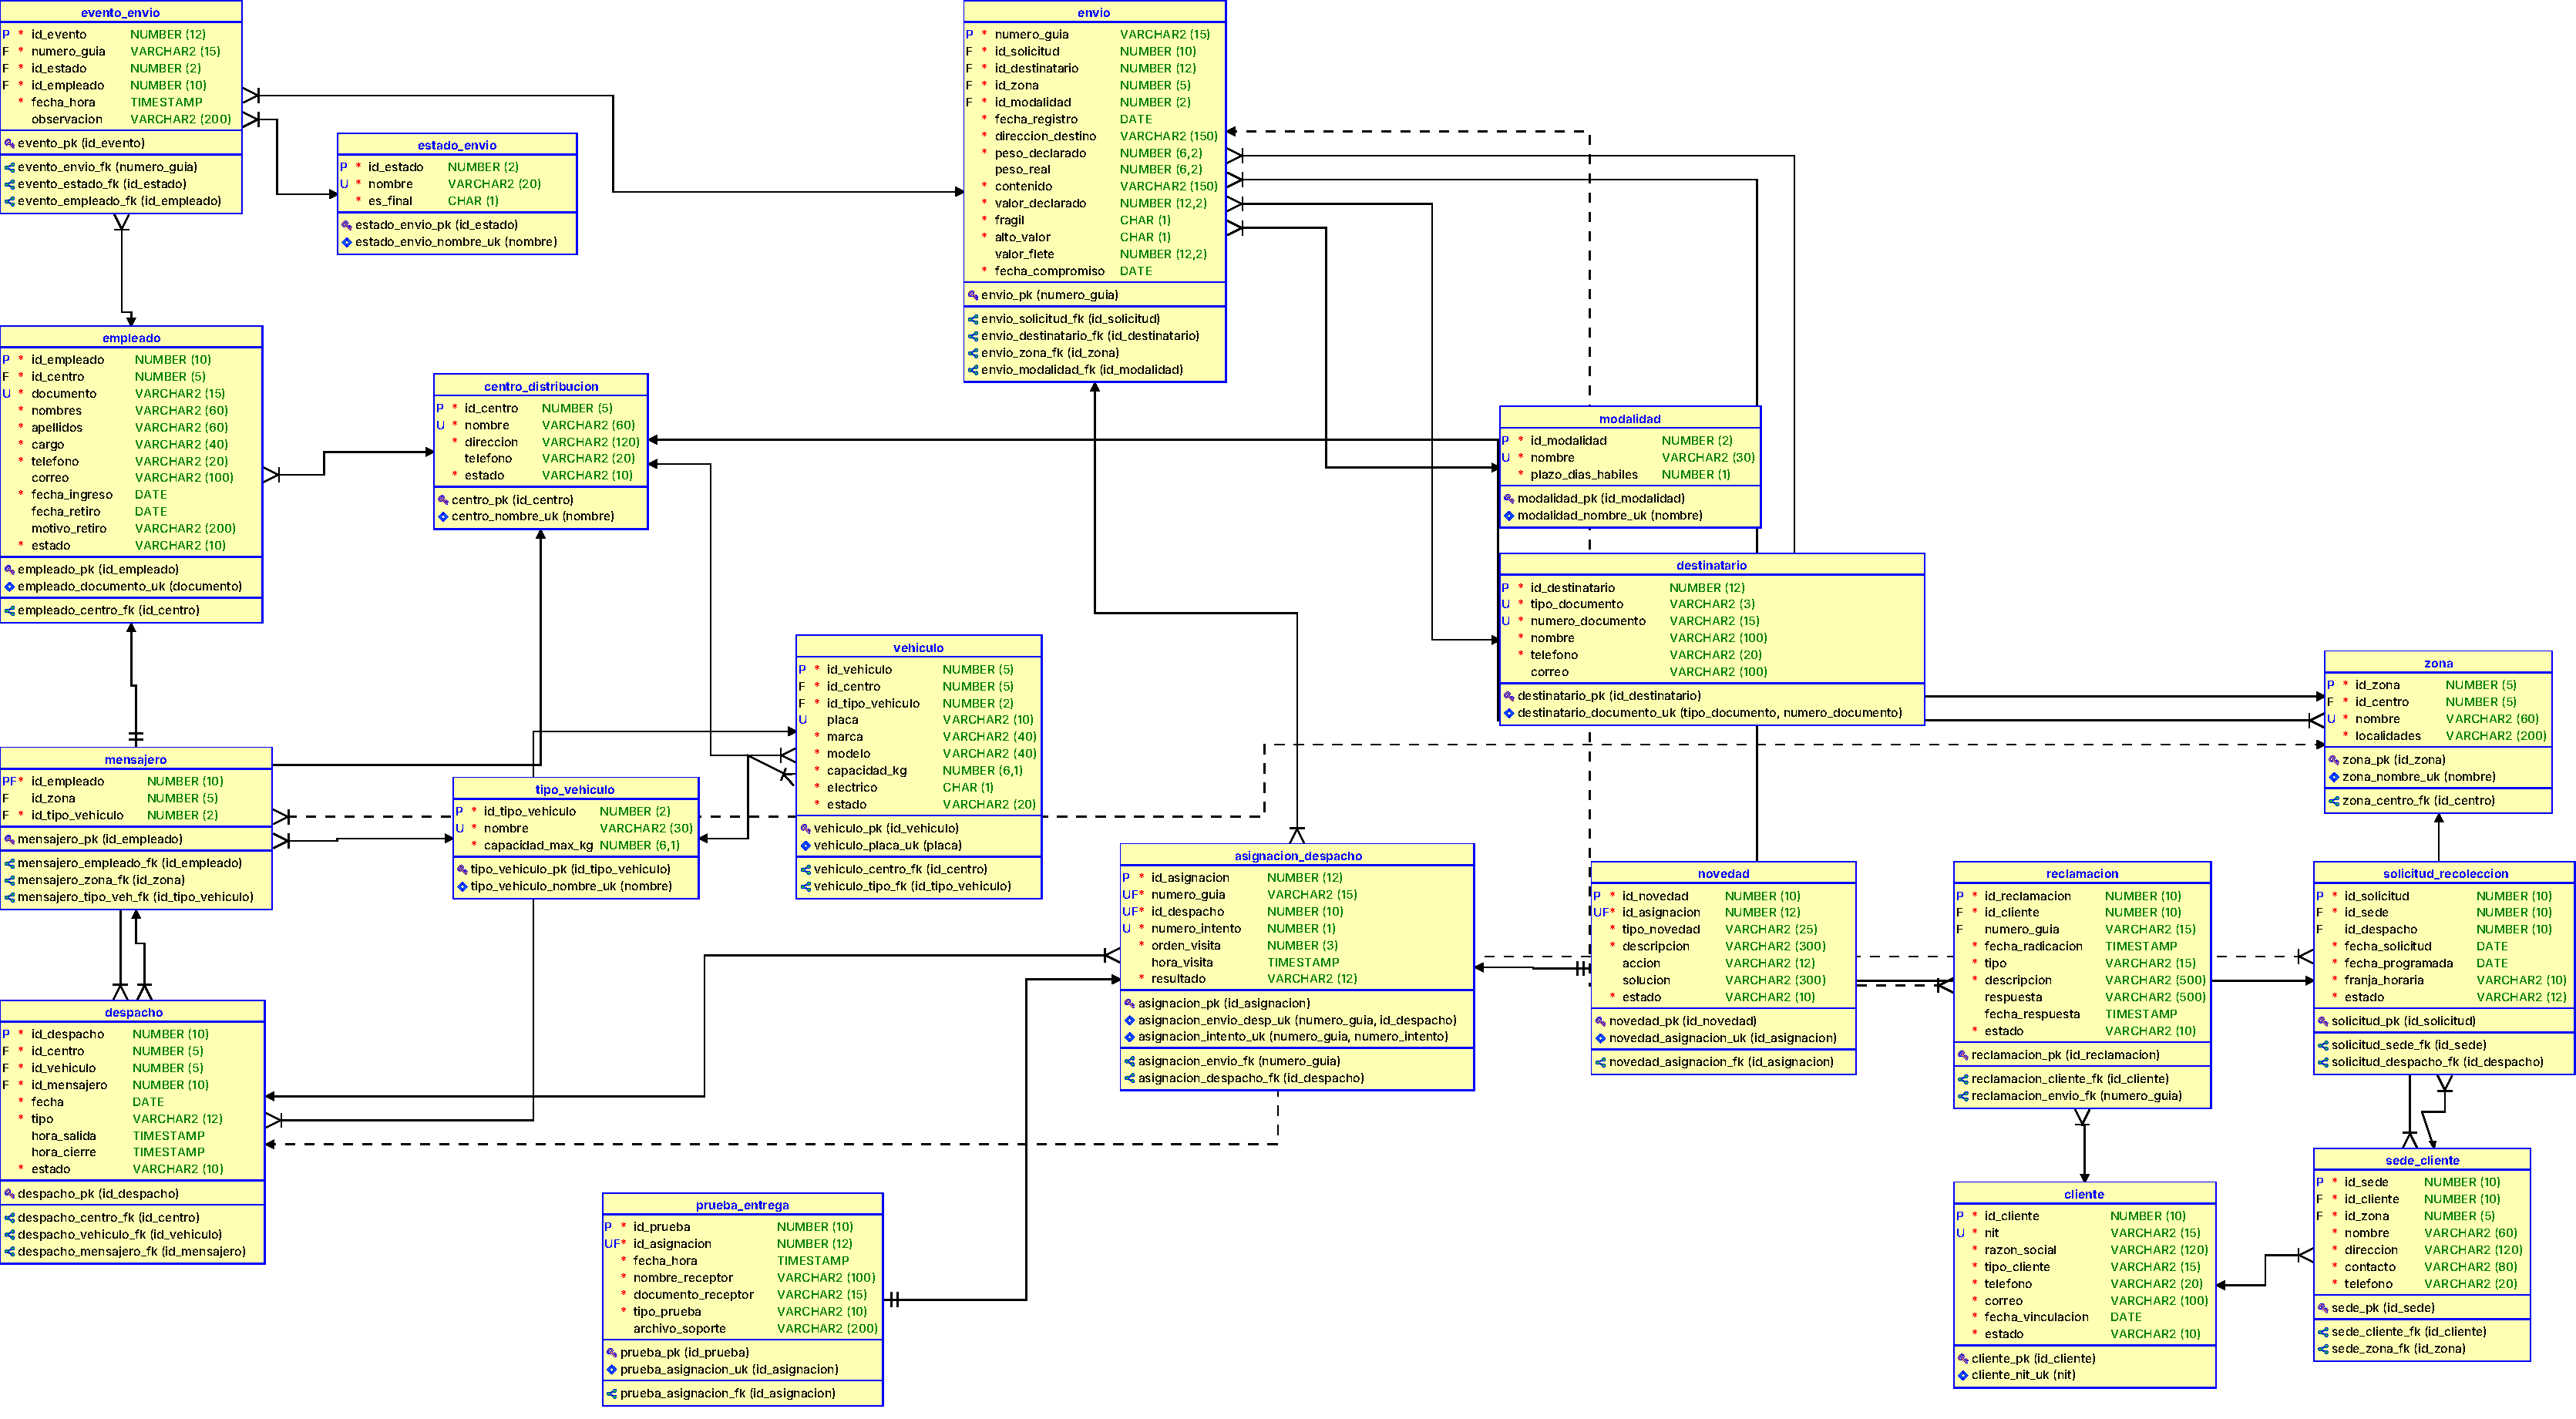
\includegraphics{figuras/datamodeler/dm_M_relacional.pdf}}
\caption{Modelo relacional del módulo en Data Modeler.}
\label{fig:dmrelacional}
\end{figure}
\par}
\end{landscape}

\paragraph{Vistas de usuario (esquema externo)}

Cada usuario del módulo accede a los datos mediante vistas que reúnen lo
que necesita sin exponerle el resto (tabla~\ref{tab:vistas}). Las vistas
también implementan el estado actual del envío (decisión 2 de
optimización) y los indicadores de operación. Por ejemplo, la vista
del estado actual reúne cada envío con su cliente, su zona y su
modalidad, y toma como estado el de su evento más reciente.

{\singlespacing\small
\begin{longtable}{L{3.6cm} L{1.4cm} L{5.6cm} L{3.8cm}}
\caption{Vistas de usuario del módulo (esquema externo).}
\label{tab:vistas}\\
\toprule
\textbf{Vista} & \textbf{Usu.} & \textbf{Propósito} & \textbf{Tablas base} \\
\midrule
\endfirsthead
\toprule
\textbf{Vista} & \textbf{Usu.} & \textbf{Propósito} & \textbf{Tablas base} \\
\midrule
\endhead
\bottomrule
\endfoot
v\_seguimiento\_envio & U3, U9 & Recorrido completo de un envío por número de guía. El cliente (U9) la consulta filtrada por su id\_cliente. & envio, solicitud\_recoleccion, sede\_cliente, evento\_envio, estado\_envio, empleado \\
\midrule
v\_estado\_actual\_envio & U1, U2, U3 & Estado actual de cada envío (el de su último evento), con cliente, zona, modalidad y fecha de compromiso. & envio, solicitud\_recoleccion, sede\_cliente, cliente, zona, modalidad, evento\_envio, estado\_envio \\
\midrule
v\_planilla\_despacho & U2, U4 & Planilla de ruta: envíos de cada despacho en orden de visita, con datos del destinatario y del mensajero. & despacho, asignacion\_despacho, envio, destinatario, zona, vehiculo, empleado \\
\midrule
v\_envios\_por\_despachar & U2 & Envíos clasificados que todavía no están en un despacho de entrega abierto, por zona y modalidad, para armar las rutas. & v\_estado\_actual\_envio, envio, asignacion\_despacho, despacho \\
\midrule
v\_novedades\_abiertas & U3 & Novedades sin cerrar, con el intento en que ocurrieron y los datos para contactar al destinatario y al cliente. & novedad, asignacion\_despacho, envio, destinatario, solicitud\_recoleccion, sede\_cliente, cliente \\
\midrule
v\_reclamaciones\_pendientes & U1, U3 & Reclamaciones abiertas, con el cliente y el envío reclamado; insumo del indicador de tiempo de respuesta. & reclamacion, cliente \\
\midrule
v\_cumplimiento\_entregas & U1 & Por centro y zona: envíos entregados y cuántos se entregaron dentro de la fecha de compromiso (indicador de OE1). & envio, zona, evento\_envio, estado\_envio \\
\end{longtable}
\par}

\subsubsection{Documentación de la BD -- Diccionario de Datos}
\label{sec:diccionario}

El diccionario de datos (tabla~\ref{tab:diccionario}) describe cada
columna del módulo: tipo de dato de Oracle, si admite nulos, su papel en
las claves y su significado. Las listas de valores permitidos y los
valores por defecto corresponden a las restricciones de dominio de la
tabla~\ref{tab:integridad}. Los estados del envío del catálogo ESTADO\_ENVIO son
REGISTRADO, RECOLECTADO, EN\_CENTRO, CLASIFICADO, EN\_RUTA, ENTREGADO,
CON\_NOVEDAD, DEVUELTO y ANULADO.
Las descripciones también se registraron en Data Modeler, en el campo
\textit{Comment in RDBMS} de cada tabla y columna. El reporte de tablas
generado por la herramienta y su comparación con este diccionario están
en el anexo~\ref{anx:dmdiccionario}.

{\singlespacing\footnotesize
\begin{longtable}{L{3.3cm} L{2.6cm} L{0.8cm} L{1.2cm} L{5.8cm}}
\caption{Diccionario de datos del módulo de operación de envíos.}
\label{tab:diccionario}\\
\toprule
\textbf{Columna} & \textbf{Tipo} & \textbf{Nulo} & \textbf{Clave} & \textbf{Descripción} \\
\midrule
\endfirsthead
\toprule
\textbf{Columna} & \textbf{Tipo} & \textbf{Nulo} & \textbf{Clave} & \textbf{Descripción} \\
\midrule
\endhead
\bottomrule
\endfoot
\multicolumn{5}{L{15.4cm}}{\textbf{centro\_distribucion} -- Centro donde se reciben, clasifican y despachan los envíos. \textit{(Estructura operativa)}} \\*
\midrule
id\_centro & NUMBER(5) & No & PK & Identificador del centro \\
nombre & VARCHAR2(60) & No & UK & Nombre del centro \\
direccion & VARCHAR2(120) & No &  & Dirección \\
telefono & VARCHAR2(20) & Sí &  & Teléfono de contacto \\
estado & VARCHAR2(10) & No &  & ACTIVO o INACTIVO; por defecto ACTIVO \\
\midrule
\multicolumn{5}{L{15.4cm}}{\textbf{zona} -- Sector de la ciudad atendido por un centro. \textit{(Estructura operativa)}} \\*
\midrule
id\_zona & NUMBER(5) & No & PK & Identificador de la zona \\
id\_centro & NUMBER(5) & No & FK & Centro que atiende la zona (ref. centro\_distribucion) \\
nombre & VARCHAR2(60) & No & UK & Nombre de la zona \\
localidades & VARCHAR2(200) & No &  & Localidades que cubre \\
\midrule
\multicolumn{5}{L{15.4cm}}{\textbf{cliente} -- Empresa que contrata el servicio. \textit{(Referencia (comercial))}} \\*
\midrule
id\_cliente & NUMBER(10) & No & PK & Identificador del cliente \\
nit & VARCHAR2(15) & No & UK & NIT \\
razon\_social & VARCHAR2(120) & No &  & Razón social \\
tipo\_cliente & VARCHAR2(15) & No &  & TIENDA\_LINEA, DROGUERIA u OFICINA \\
telefono & VARCHAR2(20) & No &  & Teléfono \\
correo & VARCHAR2(100) & No &  & Correo electrónico \\
fecha\_vinculacion & DATE & No &  & Fecha de vinculación \\
estado & VARCHAR2(10) & No &  & ACTIVO o INACTIVO; por defecto ACTIVO \\
\midrule
\multicolumn{5}{L{15.4cm}}{\textbf{sede\_cliente} -- Punto de recolección de un cliente. \textit{(Referencia (comercial))}} \\*
\midrule
id\_sede & NUMBER(10) & No & PK & Identificador de la sede \\
id\_cliente & NUMBER(10) & No & FK & Cliente dueño de la sede (ref. cliente) \\
id\_zona & NUMBER(5) & No & FK & Zona donde está la sede (ref. zona) \\
nombre & VARCHAR2(60) & No &  & Nombre de la sede \\
direccion & VARCHAR2(120) & No &  & Dirección \\
contacto & VARCHAR2(80) & No &  & Persona de contacto \\
telefono & VARCHAR2(20) & No &  & Teléfono \\
\midrule
\multicolumn{5}{L{15.4cm}}{\textbf{modalidad} -- Tipo de servicio según el tiempo de entrega. \textit{(Referencia (comercial))}} \\*
\midrule
id\_modalidad & NUMBER(2) & No & PK & Identificador \\
nombre & VARCHAR2(30) & No & UK & MISMO\_DIA, DIA\_SIGUIENTE o ESTANDAR \\
plazo\_dias\_habiles & NUMBER(1) & No &  & Plazo de entrega en días hábiles \\
\midrule
\multicolumn{5}{L{15.4cm}}{\textbf{tipo\_vehiculo} -- Catálogo de tipos de vehículo. \textit{(Referencia (flota))}} \\*
\midrule
id\_tipo\_vehiculo & NUMBER(2) & No & PK & Identificador \\
nombre & VARCHAR2(30) & No & UK & MOTOCICLETA, FURGONETA o BICICLETA\_ELECTRICA \\
capacidad\_max\_kg & NUMBER(6,1) & No &  & Carga máxima del tipo \\
\midrule
\multicolumn{5}{L{15.4cm}}{\textbf{vehiculo} -- Vehículo de la flota. \textit{(Referencia (flota))}} \\*
\midrule
id\_vehiculo & NUMBER(5) & No & PK & Identificador \\
id\_centro & NUMBER(5) & No & FK & Centro al que está asignado (ref. centro\_distribucion) \\
id\_tipo\_vehiculo & NUMBER(2) & No & FK & Tipo de vehículo (ref. tipo\_vehiculo) \\
placa & VARCHAR2(10) & Sí & UK & Placa (nula en bicicletas) \\
marca & VARCHAR2(40) & No &  & Marca \\
modelo & VARCHAR2(40) & No &  & Modelo \\
capacidad\_kg & NUMBER(6,1) & No &  & Carga máxima del vehículo \\
electrico & CHAR(1) & No &  & S o N \\
estado & VARCHAR2(20) & No &  & DISPONIBLE, EN\_MANTENIMIENTO o FUERA\_SERVICIO; por defecto DISPONIBLE \\
\midrule
\multicolumn{5}{L{15.4cm}}{\textbf{empleado} -- Persona vinculada a la empresa. \textit{(Referencia (talento humano))}} \\*
\midrule
id\_empleado & NUMBER(10) & No & PK & Identificador \\
id\_centro & NUMBER(5) & No & FK & Centro donde labora (ref. centro\_distribucion) \\
documento & VARCHAR2(15) & No & UK & Documento de identidad \\
nombres & VARCHAR2(60) & No &  & Nombres \\
apellidos & VARCHAR2(60) & No &  & Apellidos \\
cargo & VARCHAR2(40) & No &  & Cargo \\
telefono & VARCHAR2(20) & No &  & Teléfono \\
correo & VARCHAR2(100) & Sí &  & Correo electrónico \\
fecha\_ingreso & DATE & No &  & Fecha de ingreso \\
fecha\_retiro & DATE & Sí &  & Fecha de retiro \\
motivo\_retiro & VARCHAR2(200) & Sí &  & Motivo del retiro \\
estado & VARCHAR2(10) & No &  & ACTIVO o RETIRADO; por defecto ACTIVO \\
\midrule
\multicolumn{5}{L{15.4cm}}{\textbf{mensajero} -- Empleado que sale a ruta (subtipo de EMPLEADO). \textit{(Referencia (talento humano))}} \\*
\midrule
id\_empleado & NUMBER(10) & No & PK, FK & Mismo identificador del empleado (ref. empleado) \\
id\_zona & NUMBER(5) & Sí & FK & Zona fija asignada (opcional) (ref. zona) \\
id\_tipo\_vehiculo & NUMBER(2) & No & FK & Tipo de vehículo que conduce (ref. tipo\_vehiculo) \\
\midrule
\multicolumn{5}{L{15.4cm}}{\textbf{destinatario} -- Persona que recibe los envíos. \textit{(Operación de envíos)}} \\*
\midrule
id\_destinatario & NUMBER(12) & No & PK & Identificador \\
tipo\_documento & VARCHAR2(3) & No & UK & CC, CE, NIT, PAS o TI \\
numero\_documento & VARCHAR2(15) & No & UK & Número de documento \\
nombre & VARCHAR2(100) & No &  & Nombre completo \\
telefono & VARCHAR2(20) & No &  & Teléfono \\
correo & VARCHAR2(100) & Sí &  & Correo electrónico \\
\midrule
\multicolumn{5}{L{15.4cm}}{\textbf{despacho} -- Salida de un mensajero con un vehículo. \textit{(Operación de envíos)}} \\*
\midrule
id\_despacho & NUMBER(10) & No & PK & Identificador \\
id\_centro & NUMBER(5) & No & FK & Centro de origen (ref. centro\_distribucion) \\
id\_vehiculo & NUMBER(5) & No & FK & Vehículo asignado (ref. vehiculo) \\
id\_mensajero & NUMBER(10) & No & FK & Mensajero asignado (ref. mensajero) \\
fecha & DATE & No &  & Fecha del despacho \\
tipo & VARCHAR2(12) & No &  & RECOLECCION o ENTREGA \\
hora\_salida & TIMESTAMP & Sí &  & Hora de salida \\
hora\_cierre & TIMESTAMP & Sí &  & Hora de cierre de la ruta \\
estado & VARCHAR2(10) & No &  & ARMADO, EN\_RUTA o CERRADO; por defecto ARMADO \\
\midrule
\multicolumn{5}{L{15.4cm}}{\textbf{solicitud\_recoleccion} -- Pedido de recolección en una sede del cliente. \textit{(Operación de envíos)}} \\*
\midrule
id\_solicitud & NUMBER(10) & No & PK & Identificador \\
id\_sede & NUMBER(10) & No & FK & Sede donde se recoge (ref. sede\_cliente) \\
id\_despacho & NUMBER(10) & Sí & FK & Despacho de recolección (al programarla) (ref. despacho) \\
fecha\_solicitud & DATE & No &  & Fecha en que se pide \\
fecha\_programada & DATE & No &  & Fecha de recolección \\
franja\_horaria & VARCHAR2(10) & No &  & MANANA o TARDE \\
estado & VARCHAR2(12) & No &  & PENDIENTE, PROGRAMADA, ATENDIDA o NO\_ATENDIDA; por defecto PENDIENTE \\
\midrule
\multicolumn{5}{L{15.4cm}}{\textbf{envio} -- Paquete o documento identificado por su guía. \textit{(Operación de envíos)}} \\*
\midrule
numero\_guia & VARCHAR2(15) & No & PK & Número de guía \\
id\_solicitud & NUMBER(10) & No & FK & Solicitud en la que se recoge (ref. solicitud\_recoleccion) \\
id\_destinatario & NUMBER(12) & No & FK & Destinatario (ref. destinatario) \\
id\_zona & NUMBER(5) & No & FK & Zona de destino (ref. zona) \\
id\_modalidad & NUMBER(2) & No & FK & Modalidad contratada (ref. modalidad) \\
fecha\_registro & DATE & No &  & Fecha de registro \\
direccion\_destino & VARCHAR2(150) & No &  & Dirección de entrega \\
peso\_declarado & NUMBER(6,2) & No &  & Peso declarado en kg \\
peso\_real & NUMBER(6,2) & Sí &  & Peso verificado en el centro \\
contenido & VARCHAR2(150) & No &  & Descripción del contenido \\
valor\_declarado & NUMBER(12,2) & No &  & Valor declarado \\
fragil & CHAR(1) & No &  & S o N; por defecto N \\
alto\_valor & CHAR(1) & No &  & S o N; por defecto N \\
valor\_flete & NUMBER(12,2) & Sí &  & Valor cobrado por el envío \\
fecha\_compromiso & DATE & No &  & Fecha máxima de entrega \\
\midrule
\multicolumn{5}{L{15.4cm}}{\textbf{asignacion\_despacho} -- Cada intento de un envío en un despacho. \textit{(Operación de envíos)}} \\*
\midrule
id\_asignacion & NUMBER(12) & No & PK & Identificador \\
numero\_guia & VARCHAR2(15) & No & FK, UK & Envío (ref. envio) \\
id\_despacho & NUMBER(10) & No & FK, UK & Despacho (ref. despacho) \\
numero\_intento & NUMBER(1) & No & UK & 1 y 2: entrega; 3: devolución \\
orden\_visita & NUMBER(3) & No &  & Orden de visita en la ruta \\
hora\_visita & TIMESTAMP & Sí &  & Hora en que se visitó \\
resultado & VARCHAR2(12) & No &  & PENDIENTE, ENTREGADO, NOVEDAD o DEVUELTO; por defecto PENDIENTE \\
\midrule
\multicolumn{5}{L{15.4cm}}{\textbf{estado\_envio} -- Catálogo de estados del envío. \textit{(Operación de envíos)}} \\*
\midrule
id\_estado & NUMBER(2) & No & PK & Identificador \\
nombre & VARCHAR2(20) & No & UK & Nombre del estado \\
es\_final & CHAR(1) & No &  & S si el envío ya no cambia de estado; por defecto N \\
\midrule
\multicolumn{5}{L{15.4cm}}{\textbf{evento\_envio} -- Cada cambio de estado de un envío. \textit{(Operación de envíos)}} \\*
\midrule
id\_evento & NUMBER(12) & No & PK & Identificador \\
numero\_guia & VARCHAR2(15) & No & FK & Envío (ref. envio) \\
id\_estado & NUMBER(2) & No & FK & Estado al que pasa (ref. estado\_envio) \\
id\_empleado & NUMBER(10) & No & FK & Empleado responsable (ref. empleado) \\
fecha\_hora & TIMESTAMP & No &  & Fecha y hora del cambio \\
observacion & VARCHAR2(200) & Sí &  & Observación \\
\midrule
\multicolumn{5}{L{15.4cm}}{\textbf{prueba\_entrega} -- Constancia de recibo de una entrega o devolución. \textit{(Operación de envíos)}} \\*
\midrule
id\_prueba & NUMBER(10) & No & PK & Identificador \\
id\_asignacion & NUMBER(12) & No & FK, UK & Intento al que corresponde (ref. asignacion\_despacho) \\
fecha\_hora & TIMESTAMP & No &  & Fecha y hora de recibo \\
nombre\_receptor & VARCHAR2(100) & No &  & Quién recibe \\
documento\_receptor & VARCHAR2(15) & No &  & Documento de quien recibe \\
tipo\_prueba & VARCHAR2(10) & No &  & FIRMA, DOCUMENTO o FOTOGRAFIA \\
archivo\_soporte & VARCHAR2(200) & Sí &  & Ruta del archivo de soporte \\
\midrule
\multicolumn{5}{L{15.4cm}}{\textbf{novedad} -- Situación que impidió la entrega en un intento. \textit{(Operación de envíos)}} \\*
\midrule
id\_novedad & NUMBER(10) & No & PK & Identificador \\
id\_asignacion & NUMBER(12) & No & FK, UK & Intento en que ocurrió (ref. asignacion\_despacho) \\
tipo\_novedad & VARCHAR2(25) & No &  & Tipo de novedad \\
descripcion & VARCHAR2(300) & No &  & Descripción \\
accion & VARCHAR2(12) & Sí &  & REINTENTO o DEVOLUCION \\
solucion & VARCHAR2(300) & Sí &  & Solución aplicada \\
estado & VARCHAR2(10) & No &  & ABIERTA o CERRADA; por defecto ABIERTA \\
\midrule
\multicolumn{5}{L{15.4cm}}{\textbf{reclamacion} -- Inconformidad de un cliente. \textit{(Operación de envíos)}} \\*
\midrule
id\_reclamacion & NUMBER(10) & No & PK & Identificador \\
id\_cliente & NUMBER(10) & No & FK & Cliente que reclama (ref. cliente) \\
numero\_guia & VARCHAR2(15) & Sí & FK & Envío reclamado (opcional) (ref. envio) \\
fecha\_radicacion & TIMESTAMP & No &  & Fecha y hora de radicación \\
tipo & VARCHAR2(15) & No &  & ENTREGA, DANO, FACTURACION u OTRO \\
descripcion & VARCHAR2(500) & No &  & Descripción \\
respuesta & VARCHAR2(500) & Sí &  & Respuesta dada \\
fecha\_respuesta & TIMESTAMP & Sí &  & Fecha y hora de respuesta \\
estado & VARCHAR2(10) & No &  & ABIERTA, RESPONDIDA o CERRADA; por defecto ABIERTA \\
\end{longtable}
\par}

\newpage

%======================================================================
%  Capitulo 5 - Diseno fisico de bases de datos (generado por gen/cap5.py)
%======================================================================

\section{Diseño físico de bases de datos}

El diseño físico decide cómo se implementa el modelo relacional del
capítulo 4 en un sistema gestor de bases de datos concreto: tipos de
datos, generación de claves, índices, disparadores, usuarios y
permisos, dónde se guardan los datos y con qué recursos funciona la base
de datos. Como el resto del diseño detallado, se hace para el módulo
priorizado de operación de envíos (sección~\ref{sec:modulo}).

%-----------------------------------------------------------------------
\subsection{Conversión del Diseño Lógico al Diseño Físico}

\subsubsection{Modelo Relacional al Modelo Computacional (DBMS)}

\textbf{Sistema gestor de bases de datos.} Se usa Oracle Database,
uno de los gestores que indica el programa del curso (Oracle 23c o
superior), por tres razones: el modelo se construyó en Oracle SQL
Developer Data Modeler, que genera el esquema para Oracle; Oracle aplica todas las
restricciones del modelo lógico (claves, unicidad, CHECK y valores por
defecto) y permite programar en la base de datos las reglas que
dependen de otras filas; y tiene una edición gratuita, Oracle AI
Database Free, suficiente para la primera fase. Esa edición limita el
uso a dos núcleos de procesador, 2 GB de memoria y 12 GB de datos de
usuario\footnote{Oracle, \textit{Oracle AI Database Free Installation
Guide}, capítulo ``Licensing Restrictions'', 2026.}. La estimación de
la sección~\ref{sec:almacenamiento} muestra que el módulo ocupa cerca de
2,7 GB a los tres años, de modo que cabe holgadamente; cuando la
empresa supere esos límites se pasa a la edición Standard Edition 2,
que usa el mismo motor y no exige cambiar el diseño.

\textbf{Tipos de datos.} Los tipos del diccionario de datos
(tabla~\ref{tab:diccionario}) ya son tipos de Oracle; la
tabla~\ref{tab:tipos} resume el criterio con que se eligieron. La base de
datos usa el juego de caracteres AL32UTF8, y las longitudes de texto se
cuentan en caracteres y no en bytes, para que un nombre con tildes o
con eñe quepa en el tamaño definido.

{\singlespacing\small
\begin{longtable}{L{3.6cm} L{3.0cm} L{7.8cm}}
\caption{Correspondencia entre los datos del modelo y los tipos de Oracle.}
\label{tab:tipos}\\
\toprule
\textbf{Dato} & \textbf{Tipo en Oracle} & \textbf{Criterio} \\
\midrule
\endfirsthead
\toprule
\textbf{Dato} & \textbf{Tipo en Oracle} & \textbf{Criterio} \\
\midrule
\endhead
\bottomrule
\endfoot
Identificadores sustitutos & NUMBER(2) a NUMBER(12) & Tamaño según el volumen esperado: 2 dígitos para catálogos, 5 para centros, zonas y vehículos, 10 a 12 para las tablas que crecen a diario. \\
Número de guía & VARCHAR2(15) & Código alfanumérico impreso en la etiqueta: prefijo de la empresa y un consecutivo. \\
Nombres, direcciones y descripciones & VARCHAR2(n) & Longitud variable; solo ocupa el espacio del texto escrito. \\
Estados, tipos y listas de valores & VARCHAR2(10 a 25) & Valores legibles controlados con CHECK. \\
Indicadores sí/no & CHAR(1) & Valores S o N controlados con CHECK. \\
Pesos, capacidades y dinero & NUMBER(p,s) & Precisión fija: pesos con dos decimales en kg y valores con dos decimales en pesos colombianos. \\
Fechas de calendario & DATE & Fecha de registro, de compromiso, de vinculación. \\
Instantes de la operación & TIMESTAMP & Eventos, visitas y pruebas de entrega, donde importan la hora y el orden. \\
Soportes de la prueba de entrega & VARCHAR2(200) & Ruta del archivo (firma o fotografía); la imagen se guarda en el almacenamiento de archivos, no dentro de la base de datos. \\
\end{longtable}
\par}

\textbf{Generación de claves.} Las claves sustitutas se generan como
columnas de identidad, que Oracle implementa con una secuencia propia de
cada tabla; así ninguna aplicación tiene que calcular el siguiente
número. Las excepciones son tres. El número de guía lo asigna el
procedimiento de registro del envío, con el prefijo EE y un consecutivo
de 13 dígitos. La clave de MENSAJERO es la misma del empleado, porque es
un subtipo. Y los catálogos pequeños (ESTADO\_ENVIO, MODALIDAD y
TIPO\_VEHICULO) se cargan con valores fijos al instalar la base de
datos, porque las reglas y las vistas se refieren a ellos.

\textbf{Índices.} Oracle crea automáticamente un índice para cada clave
primaria y cada restricción de unicidad (32 índices), pero no para
las claves foráneas. Sin índice, cada consulta que une dos tablas por una
clave foránea, y cada verificación de que una fila no está referenciada,
recorre la tabla completa. Por eso se crea un índice para cada clave
foránea que no queda cubierta por un índice existente (22 índices)
y 5 índices adicionales para las consultas más frecuentes
(tabla~\ref{tab:indices}). En total el módulo tiene 59 índices.
Con el índice único sobre número de guía y fecha del evento, el estado
actual del envío se obtiene leyendo una sola entrada del índice, así que
no hace falta guardarlo como dato derivado en ENVIO (decisión 2 de la
optimización del diseño lógico).

{\singlespacing\small
\begin{longtable}{L{3.3cm} L{4.6cm} L{2.8cm} L{3.7cm}}
\caption{Índices que se agregan a los de las claves primarias y únicas.}
\label{tab:indices}\\
\toprule
\textbf{Tabla} & \textbf{Claves foráneas indexadas} & \textbf{Índice adicional} & \textbf{Motivo del índice adicional} \\
\midrule
\endfirsthead
\toprule
\textbf{Tabla} & \textbf{Claves foráneas indexadas} & \textbf{Índice adicional} & \textbf{Motivo del índice adicional} \\
\midrule
\endhead
\bottomrule
\endfoot
zona & id\_centro & -- &  \\
sede\_cliente & id\_cliente; id\_zona & -- &  \\
vehiculo & id\_centro; id\_tipo\_vehiculo & -- &  \\
empleado & id\_centro & -- &  \\
mensajero & id\_zona; id\_tipo\_vehiculo & -- &  \\
despacho & id\_centro; id\_vehiculo; id\_mensajero & fecha & Planilla del día y despachos abiertos. \\
solicitud\_recoleccion & id\_sede; id\_despacho & -- &  \\
envio & id\_solicitud; id\_destinatario; id\_zona; id\_modalidad & fecha\_registro & Indicadores y consultas por periodo. \\
asignacion\_despacho & id\_despacho & -- &  \\
evento\_envio & id\_estado; id\_empleado & numero\_guia, fecha\_hora (único) & Ubica el último evento de cada envío (estado actual y seguimiento) y evita dos eventos del mismo envío en el mismo instante; cubre también la clave foránea hacia ENVIO. \\
novedad & -- & estado & Novedades abiertas (vista de la mesa de servicio). \\
reclamacion & id\_cliente; numero\_guia & estado & Reclamaciones pendientes. \\
\end{longtable}
\par}

\textbf{Ciclo de vida del envío.} La regla RN12 exige que los estados de
un envío sigan un orden. La tabla~\ref{tab:transiciones} define las
transiciones permitidas; el disparador de EVENTO\_ENVIO rechaza
cualquier otra. ENTREGADO, DEVUELTO y ANULADO son estados finales: un
envío en uno de ellos no recibe más eventos.

{\singlespacing\small
\begin{longtable}{L{3.4cm} L{5.2cm} L{5.8cm}}
\caption{Transiciones permitidas entre estados del envío.}
\label{tab:transiciones}\\
\toprule
\textbf{Estado actual} & \textbf{Estados siguientes} & \textbf{Situación} \\
\midrule
\endfirsthead
\toprule
\textbf{Estado actual} & \textbf{Estados siguientes} & \textbf{Situación} \\
\midrule
\endhead
\bottomrule
\endfoot
(sin eventos) & REGISTRADO & Toda guía nace registrada (RN12). \\
REGISTRADO & RECOLECTADO, ANULADO & Se recoge en la sede o se anula antes de recogerlo. \\
RECOLECTADO & EN\_CENTRO, ANULADO & Llega al centro de distribución. \\
EN\_CENTRO & CLASIFICADO, ANULADO & Se pesa, se verifica y se clasifica por zona. \\
CLASIFICADO & EN\_RUTA, ANULADO & Sale en un despacho de entrega. \\
EN\_RUTA & ENTREGADO, CON\_NOVEDAD, DEVUELTO & Resultado del intento; DEVUELTO solo en el tercer intento (RN07). \\
CON\_NOVEDAD & EN\_RUTA & Reintento en un nuevo despacho. \\
ENTREGADO, DEVUELTO, ANULADO & -- & Estados finales. \\
\end{longtable}
\par}

\textbf{Disparadores y procedimientos.} Las reglas de negocio que
dependen de otras filas o tablas (tabla~\ref{tab:reglasnegocio}) se
programan en la base de datos, de modo que se cumplen sin importar qué
aplicación registre los datos. La tabla~\ref{tab:disparadores} muestra
qué hace cada uno; todos rechazan la operación con un mensaje que
explica la regla incumplida.

{\singlespacing\small
\begin{longtable}{L{4.0cm} L{3.4cm} L{5.4cm} L{1.4cm}}
\caption{Disparadores y procedimiento del módulo.}
\label{tab:disparadores}\\
\toprule
\textbf{Objeto} & \textbf{Tabla y momento} & \textbf{Qué verifica o hace} & \textbf{Reglas} \\
\midrule
\endfirsthead
\toprule
\textbf{Objeto} & \textbf{Tabla y momento} & \textbf{Qué verifica o hace} & \textbf{Reglas} \\
\midrule
\endhead
\bottomrule
\endfoot
Procedimiento de registro del envío & ENVIO y EVENTO\_ENVIO & Genera el número de guía, inserta el envío y su evento REGISTRADO en una sola transacción, y crea el destinatario si no existe. & RN02, RN12 \\
Disparador de solicitud & SOLICITUD\_RECOLECCION, antes de insertar & El cliente dueño de la sede está ACTIVO. & RN15 \\
Disparador de despacho & DESPACHO, antes de insertar o cambiar vehículo o mensajero & El vehículo está DISPONIBLE, el mensajero está ACTIVO y el vehículo es del tipo que conduce el mensajero. & RN10, RN11 \\
Disparador de asignación & ASIGNACION\_DESPACHO, antes de insertar & El despacho es de entrega y no está cerrado; el intento \textit{n} solo se crea si los anteriores terminaron en NOVEDAD; el tercero es la devolución. & RN07 \\
Disparador de resultado & ASIGNACION\_DESPACHO, antes de actualizar el resultado & ENTREGADO o DEVUELTO exigen una prueba de entrega del intento; NOVEDAD exige la novedad registrada; el tercer intento solo puede terminar en DEVUELTO. & RN05, RN07, RN08 \\
Disparador de prueba & PRUEBA\_ENTREGA, antes de insertar & Si el envío es frágil o de alto valor, el documento de quien recibe es el del destinatario. & RN06 \\
Disparador de evento & EVENTO\_ENVIO, antes de insertar & La transición está permitida (tabla~\ref{tab:transiciones}) y ENTREGADO o DEVUELTO corresponden a un intento con ese resultado. & RN05, RN12 \\
\end{longtable}
\par}

\textbf{Usuarios, roles y permisos.} Cada grupo de usuarios del módulo
tiene un rol con los permisos de la tabla~\ref{tab:permisos} traducidos a
privilegios: crear es insertar, actualizar es modificar y leer es
consultar. Ningún rol tiene permiso de borrar (RN16). Las tablas
pertenecen a un esquema propietario, BD\_ENLACE\_EXPRESS, con el que no
trabaja ningún usuario. El administrador de la base de datos crea los objetos,
carga los catálogos y, mientras se integran los módulos M2 a M4,
registra y actualiza los datos de referencia (clientes, sedes,
vehículos y empleados) a solicitud de las áreas dueñas
(tabla~\ref{tab:interfaces}). Los usuarios no tienen una cuenta propia
en la base de datos. El servidor de aplicaciones se conecta con una
cuenta de servicio por rol (cinco cuentas, como svc\_mesa y svc\_centro,
cada una con solo su rol) y elige la cuenta según el rol del usuario que
inició sesión en la aplicación; las consultas públicas del portal, que se
hacen antes de iniciar sesión, usan la cuenta de menor privilegio, la del
rol cliente. En cada conexión, el servidor fija además el identificador
de cliente de la sesión de Oracle con el usuario real, de modo que la
base de datos sabe quién hizo cada operación y puede auditarla. Así no
hay que crear ni administrar en la base de datos una cuenta por cada
empleado y cliente: el control por usuario lo hace la aplicación (por
ejemplo, el mensajero solo ve sus despachos y el cliente solo sus
envíos), y Oracle sigue limitando, mediante la cuenta de servicio, lo que
cada rol puede hacer.

{\singlespacing\small
\begin{longtable}{L{2.3cm} L{0.9cm} L{3.6cm} L{3.6cm} L{3.5cm}}
\caption{Roles de la base de datos y sus privilegios.}
\label{tab:roles}\\
\toprule
\textbf{Rol} & \textbf{Usu.} & \textbf{Inserta} & \textbf{Modifica} & \textbf{Consulta} \\
\midrule
\endfirsthead
\toprule
\textbf{Rol} & \textbf{Usu.} & \textbf{Inserta} & \textbf{Modifica} & \textbf{Consulta} \\
\midrule
\endhead
\bottomrule
\endfoot
rol\_gerencia & U1 & -- & -- & Tablas que alimentan los indicadores y vistas del módulo \\
rol\_centro & U2 & centro\_distribucion, zona, despacho, asignacion\_despacho, evento\_envio & centro\_distribucion, zona, despacho, asignacion\_despacho, solicitud\_recoleccion, envio, empleado, mensajero & Catálogos, sedes, vehículos, empleados; vistas de planilla y envíos por despachar \\
rol\_mesa & U3 & solicitud\_recoleccion, envio, destinatario, evento\_envio, reclamacion & envio, destinatario, novedad, reclamacion & Clientes, sedes, zonas, catálogos; vistas de seguimiento, novedades y reclamaciones \\
rol\_mensajero & U4 & evento\_envio, prueba\_entrega, novedad & solicitud\_recoleccion, asignacion\_despacho, envio & Sedes de recolección, su despacho y la vista de planilla \\
rol\_cliente & U9 & -- & -- & Vista de seguimiento, filtrada por el portal \\
\end{longtable}
\par}

\textbf{Espacios de tablas.} Las tablas y los índices se guardan en
espacios de tablas separados (tabla~\ref{tab:tablespaces}), lo que
permite vigilar el crecimiento de cada uno y, si se cambia de servidor,
ubicarlos en discos distintos. Su tamaño inicial cubre el primer año de
la estimación y crecen automáticamente hasta un máximo que respeta el
límite de 12 GB de la edición gratuita.

{\singlespacing\small
\begin{longtable}{L{3.6cm} L{3.8cm} L{1.6cm} L{2.2cm} L{1.6cm}}
\caption{Espacios de tablas del módulo.}
\label{tab:tablespaces}\\
\toprule
\textbf{Espacio de tablas} & \textbf{Contenido} & \textbf{Inicial} & \textbf{Aumento} & \textbf{Máximo} \\
\midrule
\endfirsthead
\toprule
\textbf{Espacio de tablas} & \textbf{Contenido} & \textbf{Inicial} & \textbf{Aumento} & \textbf{Máximo} \\
\midrule
\endhead
\bottomrule
\endfoot
TS\_ENLACE\_DATOS & Las 19 tablas & 500 MB & 100 MB & 7 GB \\
TS\_ENLACE\_INDICES & Los 59 índices & 300 MB & 100 MB & 4 GB \\
\end{longtable}
\par}

%-----------------------------------------------------------------------
\subsubsection{Organización física de los datos}

\paragraph{Almacenamiento (Centralizado o Distribuido)}
\label{sec:almacenamiento}

El almacenamiento es \textbf{centralizado}: una sola base de datos
guarda la información de todos los centros. Se descarta el
almacenamiento distribuido porque la empresa opera en una sola ciudad;
un envío pasa por varios centros y zonas y su historial debe estar
completo en un solo lugar; la política de sistema único desde el inicio
(capítulo 1) busca precisamente no repartir los datos; y el volumen
esperado lo maneja sin dificultad un solo servidor. Distribuir los datos
obligaría a replicarlos y a mantener la consistencia entre sitios sin
ningún beneficio para este tamaño de operación.

Para dimensionar el almacenamiento se partió de los datos del
capítulo 1 con los siguientes supuestos: 900 envíos por día hábil
(25 mensajeros con unas 36 visitas cada uno), 300 días hábiles al año
(lunes a sábado) y un crecimiento del 25\,\% anual. Por cada envío se
registran en promedio 6,2 eventos, 1,12 asignaciones a despacho, una
prueba de entrega y 0,12 novedades; el 60\,\% de los envíos va a un
destinatario nuevo, una solicitud de recolección agrupa unos seis envíos
y cada mensajero sale en dos despachos al día. El tamaño de cada fila se
calculó con los tipos del diccionario de datos, suponiendo los textos
llenos a la mitad, y el de los bloques con un 10\,\% de espacio libre
para actualizaciones. La tabla~\ref{tab:volumen} muestra el resultado
para las tablas que crecen con la operación; las demás son tablas
maestras y de catálogo de pocos cientos de filas.

{\singlespacing\small
\begin{longtable}{L{3.4cm} >{\raggedleft\arraybackslash}p{1.4cm} >{\raggedleft\arraybackslash}p{2.0cm} >{\raggedleft\arraybackslash}p{2.0cm} >{\raggedleft\arraybackslash}p{2.0cm} >{\raggedleft\arraybackslash}p{2.0cm}}
\caption{Estimación del volumen de las tablas que crecen con la operación.}
\label{tab:volumen}\\
\toprule
\textbf{Tabla} & \textbf{Bytes por fila} & \textbf{Filas año 1} & \textbf{Filas a 3 años} & \textbf{Datos a 3 años (MB)} & \textbf{Índices a 3 años (MB)} \\
\midrule
\endfirsthead
\toprule
\textbf{Tabla} & \textbf{Bytes por fila} & \textbf{Filas año 1} & \textbf{Filas a 3 años} & \textbf{Datos a 3 años (MB)} & \textbf{Índices a 3 años (MB)} \\
\midrule
\endhead
\bottomrule
\endfoot
evento\_envio & 144 & 1.674.000 & 6.382.125 & 987,2 & 685,6 \\
envio & 234 & 270.000 & 1.029.375 & 258,7 & 137,4 \\
prueba\_entrega & 198 & 270.000 & 1.029.375 & 218,9 & 49,0 \\
destinatario & 136 & 162.000 & 617.625 & 90,2 & 32,2 \\
asignacion\_despacho & 54 & 302.400 & 1.152.900 & 66,9 & 129,2 \\
novedad & 348 & 32.400 & 123.525 & 46,2 & 8,5 \\
solicitud\_recoleccion & 55 & 45.000 & 171.562 & 10,1 & 11,8 \\
reclamacion & 567 & 2.700 & 10.294 & 6,3 & 0,9 \\
despacho & 74 & 15.000 & 57.188 & 4,5 & 6,3 \\
\midrule
\textbf{Total (19 tablas)} & & & & \textbf{1689,3} & \textbf{1061,0} \\
\end{longtable}
\par}

La base de datos del módulo ocupa unos 0,7 GB al final del primer
año y 2,7 GB a los tres años, incluidos los índices. EVENTO\_ENVIO es
la tabla más grande, porque cada envío deja varios eventos. Las
fotografías y firmas de las pruebas de entrega (unos 200 KB cada una,
cerca de 51 GB al año) se guardan en un almacenamiento de archivos
aparte, y la base de datos solo conserva su ruta.

\textbf{Copias de seguridad.} La base de datos trabaja en modo
ARCHIVELOG, que conserva el registro de todos los cambios. Se hace una
copia completa semanal y una incremental diaria con RMAN, la
herramienta de copias de Oracle, y se copian los registros de cambios
cada hora; las copias se guardan fuera del servidor durante 30 días.
Con ello se puede recuperar la base de datos hasta la última hora de
operación. Además, cada mes se exporta el esquema con Data Pump como
respaldo lógico.

\paragraph{Procesamiento (Centralizado o Distribuido)}

El procesamiento también es \textbf{centralizado}, en una arquitectura
cliente-servidor de tres niveles físicos. Los usuarios trabajan en
aplicaciones cliente (web para el centro, la mesa de servicio y la
gerencia; móvil para los mensajeros; portal para los clientes); estas
se comunican con un servidor de aplicaciones que expone servicios web,
y solo ese servidor se conecta a la base de datos. Dentro del servidor
de aplicaciones, el software se organiza en capas lógicas (casos de
uso, dominio y acceso a datos), como se justifica en la
sección~\ref{sec:arquitectura}. Las reglas de negocio se verifican en
la capa de dominio y, como garantía final, en la base de datos
(restricciones, disparadores y procedimientos), así que se cumplen
igual sin importar qué aplicación registre la operación.

La carga es baja para un solo servidor. Con los supuestos anteriores,
la operación genera unas 9.000 filas nuevas por día, la mayoría
eventos; si el 20\,\% se concentra en la hora de mayor actividad, son
menos de una inserción por segundo, con unos 35 usuarios internos
conectados al tiempo más las consultas del portal. Como los mensajeros
pueden quedarse sin señal en la ruta, la aplicación móvil guarda los
registros en el teléfono y los envía al recuperar la conexión, con la
hora real del evento.

%-----------------------------------------------------------------------
\subsubsection{Recursos Hardware, Software, Aplicaciones y BD, Comunicaciones, Ingeniería Web}

\textbf{Hardware.} La tabla~\ref{tab:hardware} resume los equipos. Los
servidores se contratan como máquinas virtuales en la nube, lo que evita
comprar equipos para una empresa que apenas inicia y permite ampliarlos
cuando crezca la operación.

{\singlespacing\small
\begin{longtable}{L{3.4cm} L{1.4cm} L{9.6cm}}
\caption{Recursos de hardware.}
\label{tab:hardware}\\
\toprule
\textbf{Recurso} & \textbf{Cant.} & \textbf{Características y uso} \\
\midrule
\endfirsthead
\toprule
\textbf{Recurso} & \textbf{Cant.} & \textbf{Características y uso} \\
\midrule
\endhead
\bottomrule
\endfoot
Servidor de base de datos & 1 & Máquina virtual con 2 núcleos, 8 GB de memoria y 100 GB de disco de estado sólido (base de datos, registros de cambios y copias locales). \\
Servidor de aplicaciones & 1 & Máquina virtual con 2 núcleos y 4 GB de memoria; atiende las aplicaciones web, la móvil y el portal. \\
Almacenamiento de archivos & 1 & Almacenamiento en la nube para fotografías y firmas de las pruebas de entrega y para las copias de seguridad (unos 51 GB al año más las copias). \\
Computadores de escritorio & 10 & Puestos del personal del centro, la mesa de servicio y la gerencia. \\
Teléfonos inteligentes & 25 & Uno por mensajero, con cámara, GPS y plan de datos, para la aplicación móvil. \\
Lectores de código de barras & 3 & Lectura de la guía al recibir, clasificar y despachar los paquetes en el centro. \\
Impresoras de etiquetas & 2 & Impresión de la etiqueta con el número de guía. \\
Equipos de red & 1 & Enrutador con cortafuegos en el centro de distribución. \\
\end{longtable}
\par}

\textbf{Software.} La tabla~\ref{tab:software} lista el software de la
base de datos y del servidor.

{\singlespacing\small
\begin{longtable}{L{3.6cm} L{4.6cm} L{6.2cm}}
\caption{Recursos de software.}
\label{tab:software}\\
\toprule
\textbf{Función} & \textbf{Software} & \textbf{Uso} \\
\midrule
\endfirsthead
\toprule
\textbf{Función} & \textbf{Software} & \textbf{Uso} \\
\midrule
\endhead
\bottomrule
\endfoot
Gestor de bases de datos & Oracle AI Database Free (después, Standard Edition 2) & Motor de la base de datos del módulo. \\
Sistema operativo & Oracle Linux & Sistema de los dos servidores. \\
Modelado & Oracle SQL Developer Data Modeler & Modelos conceptual, lógico y físico; diccionario de datos. \\
Administración y consultas & Oracle SQL Developer & Creación de objetos, consultas, informes y administración. \\
Servidor de aplicaciones & Aplicación propia con acceso a datos por JDBC & Implementa las capas de casos de uso, dominio y datos, y expone los servicios web que usan las aplicaciones (sección~\ref{sec:arquitectura}). \\
Copias de seguridad & RMAN y Data Pump & Copias físicas y exportaciones lógicas; vienen con la base de datos. \\
\end{longtable}
\par}

\textbf{Aplicaciones y base de datos.} Cada aplicación atiende a un grupo
de usuarios y se conecta con el rol de ese grupo
(tabla~\ref{tab:aplicaciones}). Las aplicaciones completas no forman parte del alcance del proyecto
(sección~\ref{sec:modulo}); el prototipo funcional
(sección~\ref{sec:prototipo}) demuestra sus funciones principales sobre
la base de datos del módulo en una sola aplicación web, con una sección
para cada grupo de usuarios y el portal público de rastreo.

{\singlespacing\small
\begin{longtable}{L{3.6cm} L{1.0cm} L{2.6cm} L{7.2cm}}
\caption{Aplicaciones que usan la base de datos.}
\label{tab:aplicaciones}\\
\toprule
\textbf{Aplicación} & \textbf{Usu.} & \textbf{Rol} & \textbf{Funciones principales} \\
\midrule
\endfirsthead
\toprule
\textbf{Aplicación} & \textbf{Usu.} & \textbf{Rol} & \textbf{Funciones principales} \\
\midrule
\endhead
\bottomrule
\endfoot
Aplicación de operación (web) & U2 & rol\_centro & Centros y zonas, recepción y clasificación, armado y cierre de despachos. \\
Aplicación de mesa de servicio (web) & U3 & rol\_mesa & Solicitudes, registro de envíos, novedades, consultas y reclamaciones. \\
Aplicación del mensajero (móvil) & U4 & rol\_mensajero & Planilla del día, recolecciones, eventos, pruebas de entrega con foto o firma y novedades; funciona sin conexión. \\
Tablero de indicadores (web) & U1 & rol\_gerencia & Indicadores de cumplimiento, novedades y reclamaciones. \\
Portal de seguimiento (web) & U9 & rol\_cliente & Consulta del estado y el recorrido de los envíos del cliente. \\
\end{longtable}
\par}

\textbf{Comunicaciones.} El centro de distribución tiene una conexión a
internet de fibra óptica y una conexión móvil de respaldo; los
mensajeros usan los datos móviles del teléfono. Todo el tráfico entre
las aplicaciones y el servidor de aplicaciones viaja cifrado (HTTPS). La
base de datos no se expone a internet: está en una red privada a la que
solo llegan el servidor de aplicaciones y, para administración, los
equipos autorizados mediante una red privada virtual (VPN).

\textbf{Ingeniería web.} Las aplicaciones web y el portal son
adaptables a la pantalla (computador o teléfono) y consumen los
servicios web del servidor de aplicaciones en formato JSON. Cada usuario
inicia sesión con su cuenta, y la aplicación solo le muestra las
opciones de su rol. El portal de clientes es la única parte pública:
permite consultar un envío con su número de guía y, con inicio de
sesión, todos los envíos del cliente. Los servicios registran quién
hizo cada operación, lo que complementa el responsable que ya guarda
cada evento del envío.

\newpage

%======================================================================
%  Capitulo 6 - Desarrollo proyecto de bases de datos (generado por gen/cap6.py)
%======================================================================

\section{Desarrollo proyecto de bases de datos}

Este capítulo define cómo se usará la base de datos del módulo de
operación de envíos: expresa en álgebra relacional y en SQL las
consultas que necesitan sus usuarios, y especifica las tablas,
relaciones, transacciones e informes. Luego presenta el prototipo
funcional (sección~\ref{sec:prototipo}): su arquitectura, la creación de
la base de datos del módulo en el gestor, los datos de prueba, los
resultados de las consultas, las transacciones y los informes, y la
aplicación web que demuestra los casos de uso.

\subsection{Algebra relacional de consultas MySQL}
\label{sec:algebra}

El álgebra relacional describe una consulta como una secuencia de
operaciones sobre relaciones, independiente del gestor de bases de
datos; SQL es la forma de escribirla para que el gestor la ejecute. En
esta sección se expresan en álgebra relacional y en SQL diez consultas
que responden a necesidades de los usuarios del módulo
(sección~\ref{sec:usuarios}). Entre todas usan las operaciones del
álgebra que resume la tabla~\ref{tab:operadores}.

La notación es la del texto guía del curso\footnote{A. Silberschatz,
H. F. Korth y S. Sudarshan, \textit{Fundamentos de bases de datos},
5.ª ed., McGraw-Hill, 2006, capítulos 2 y 3.}. Las relaciones se
escriben con el nombre de su tabla en mayúsculas, como en el esquema
relacional de la sección~\ref{sec:esquemarel}. La reunión natural
($\bowtie$) combina dos relaciones por sus atributos de igual nombre;
en este modelo esos atributos son las claves foráneas, que llevan el
mismo nombre que la clave primaria a la que apuntan. Cuando dos
relaciones comparten además otro atributo (por ejemplo, nombre o
estado), se renombra o se proyecta antes de reunirlas, y cuando la
clave foránea tiene otro nombre se usa una reunión theta. Para que las
expresiones se lean con facilidad, se escriben por pasos: cada paso
guarda un resultado intermedio con la asignación ($\leftarrow$) y el
último da la respuesta.

Cada consulta se escribe también en SQL estándar, válido tanto en
MySQL, que nombra la plantilla del proyecto, como en Oracle, el gestor
elegido en el capítulo 5. Los valores entre comillas (un número de
guía, un despacho, un rango de fechas) son ejemplos de los datos de
entrada que el usuario indica en cada caso. Su ejecución sobre la base
de datos hace parte del prototipo funcional
(sección~\ref{sec:prototipo}).

{\singlespacing\small
\begin{longtable}{L{2.4cm} L{2.4cm} L{5.6cm} L{4.0cm}}
\caption{Operaciones del álgebra relacional usadas en las consultas.}
\label{tab:operadores}\\
\toprule
\textbf{Notación} & \textbf{Operación} & \textbf{Resultado} & \textbf{Equivalente en SQL} \\
\midrule
\endfirsthead
\toprule
\textbf{Notación} & \textbf{Operación} & \textbf{Resultado} & \textbf{Equivalente en SQL} \\
\midrule
\endhead
\bottomrule
\endfoot
$\sigma_{P}(r)$ & Selección & Tuplas de r que cumplen el predicado P & WHERE \\
$\Pi_{A}(r)$ & Proyección & Atributos A de r, sin tuplas repetidas & SELECT A \\
$r \bowtie s$ & Reunión natural & Combina las tuplas de r y s que coinciden en los atributos de igual nombre & JOIN \dots\ ON (atributos comunes) \\
$r \bowtie_{\theta} s$ & Reunión theta & Combina las tuplas de r y s que cumplen la condición $\theta$ & JOIN \dots\ ON $\theta$ \\
$r \cup s$ & Unión & Tuplas que están en r o en s & UNION \\
$r - s$ & Diferencia & Tuplas de r que no están en s & NOT IN, NOT EXISTS, MINUS \\
$r \div s$ & División & Valores de r que se combinan con todas las tuplas de s & GROUP BY con HAVING COUNT \\
$_{G}\mathcal{G}_{F}(r)$ & Agregación & Agrupa r por los atributos G y calcula las funciones F (count, max, \dots) & GROUP BY, funciones de grupo \\
$\rho_{x(A)}(E)$ & Renombre & El resultado de E con nombre x y atributos A & Alias (AS) \\
$x \leftarrow E$ & Asignación & Guarda el resultado de E con el nombre x & Subconsulta o vista \\
\end{longtable}
\par}

\subsubsection{C1. Datos de un envío}
\label{q:C1}
\textit{Usuarios:} U3. \textit{Operaciones:} selección y proyección. La mesa de servicio consulta los datos de un envío a partir de su número de guía.

\begin{center}\adjustbox{max width=\linewidth}{$\displaystyle\begin{array}{l}E \leftarrow \sigma_{\text{numero\_guia} = \text{'EE0000000000003'}}(\text{ENVIO}) \\[4pt] \Pi_{\text{numero\_guia, fecha\_registro, fecha\_compromiso, peso\_real, fragil, alto\_valor}}(E)\end{array}$}\end{center}

\begin{lstlisting}[style=sqlpro]
SELECT numero_guia, fecha_registro, fecha_compromiso,
       peso_real, fragil, alto_valor
FROM   envio
WHERE  numero_guia = 'EE0000000000003'
\end{lstlisting}


\subsubsection{C2. Recorrido de un envío}
\label{q:C2}
\textit{Usuarios:} U3, U9. \textit{Operaciones:} selección, reunión natural y proyección. Muestra los eventos de un envío en orden, con el nombre del estado y el empleado responsable.

\begin{center}\adjustbox{max width=\linewidth}{$\displaystyle\begin{array}{l}E \leftarrow \sigma_{\text{numero\_guia} = \text{'EE0000000000003'}}(\text{EVENTO\_ENVIO}) \\[4pt] R \leftarrow E \bowtie \text{ESTADO\_ENVIO} \bowtie \text{EMPLEADO} \\[4pt] \Pi_{\text{fecha\_hora, nombre, nombres, observacion}}(R)\end{array}$}\end{center}

\begin{lstlisting}[style=sqlpro]
SELECT ev.fecha_hora, es.nombre AS estado,
       em.nombres AS responsable, ev.observacion
FROM   evento_envio ev
JOIN   estado_envio es ON es.id_estado   = ev.id_estado
JOIN   empleado em     ON em.id_empleado = ev.id_empleado
WHERE  ev.numero_guia = 'EE0000000000003'
ORDER  BY ev.fecha_hora
\end{lstlisting}
El orden (ORDER BY) no es una operación del álgebra relacional, porque una relación es un conjunto sin orden; se aplica al presentar el resultado.


\subsubsection{C3. Planilla de un despacho}
\label{q:C3}
\textit{Usuarios:} U2, U4. \textit{Operaciones:} renombre, selección, reunión natural y proyección. Lista los envíos asignados a un despacho en el orden de visita, con el destinatario, la dirección y la zona.

\begin{center}\adjustbox{max width=\linewidth}{$\displaystyle\begin{array}{l}Z \leftarrow \rho_{\text{Z(id\_zona, id\_centro, zona, localidades)}}(\text{ZONA}) \\[4pt] R \leftarrow \sigma_{\text{id\_despacho} = \text{15}}(\text{ASIGNACION\_DESPACHO}) \bowtie \text{ENVIO} \bowtie \text{DESTINATARIO} \bowtie Z \\[4pt] \Pi_{\text{orden\_visita, numero\_guia, nombre, direccion\_destino, zona, resultado}}(R)\end{array}$}\end{center}

\begin{lstlisting}[style=sqlpro]
SELECT a.orden_visita, a.numero_guia, d.nombre AS destinatario,
       e.direccion_destino, z.nombre AS zona, a.resultado
FROM   asignacion_despacho a
JOIN   envio e        ON e.numero_guia     = a.numero_guia
JOIN   destinatario d ON d.id_destinatario = e.id_destinatario
JOIN   zona z         ON z.id_zona         = e.id_zona
WHERE  a.id_despacho = 15
ORDER  BY a.orden_visita
\end{lstlisting}
ZONA y DESTINATARIO tienen ambos un atributo nombre; si no se renombra uno de ellos, la reunión natural exigiría que fueran iguales. En SQL ese papel lo cumplen los alias.


\subsubsection{C4. Envíos clasificados sin asignar}
\label{q:C4}
\textit{Usuarios:} U2. \textit{Operaciones:} selección, reunión natural, proyección y diferencia. Encuentra los envíos que ya fueron clasificados pero todavía no se han asignado a ningún despacho de entrega.

\begin{center}\adjustbox{max width=\linewidth}{$\displaystyle\begin{array}{l}C \leftarrow \Pi_{\text{numero\_guia}}(\text{EVENTO\_ENVIO} \bowtie \sigma_{\text{nombre} = \text{'CLASIFICADO'}}(\text{ESTADO\_ENVIO})) \\[4pt] S \leftarrow \Pi_{\text{numero\_guia}}(\text{ASIGNACION\_DESPACHO}) \\[4pt] C - S\end{array}$}\end{center}

\begin{lstlisting}[style=sqlpro]
SELECT ev.numero_guia
FROM   evento_envio ev
JOIN   estado_envio es ON es.id_estado = ev.id_estado
WHERE  es.nombre = 'CLASIFICADO'
AND    ev.numero_guia NOT IN (SELECT numero_guia
                              FROM   asignacion_despacho)
\end{lstlisting}
La diferencia se escribe con NOT IN, que funciona igual en MySQL y en Oracle; Oracle también la ofrece con el operador MINUS.


\subsubsection{C5. Envíos por zona y modalidad}
\label{q:C5}
\textit{Usuarios:} U1. \textit{Operaciones:} selección, renombre, reunión natural y agregación. Cuenta los envíos registrados en un periodo por zona de destino y modalidad.

\begin{center}\adjustbox{max width=\linewidth}{$\displaystyle\begin{array}{l}Z \leftarrow \rho_{\text{Z(id\_zona, id\_centro, zona, localidades)}}(\text{ZONA}) \\[4pt] M \leftarrow \rho_{\text{M(id\_modalidad, modalidad, plazo\_dias\_habiles)}}(\text{MODALIDAD}) \\[4pt] R \leftarrow \sigma_{\text{fecha\_registro} \geq \text{'2026-11-01'} \wedge \text{fecha\_registro} \leq \text{'2026-11-30'}}(\text{ENVIO}) \bowtie Z \bowtie M \\[4pt] {}_{\text{zona, modalidad}}\mathcal{G}_{\text{count}(\text{numero\_guia}) \text{ as } \text{envios}}(R)\end{array}$}\end{center}

\begin{lstlisting}[style=sqlpro]
SELECT z.nombre AS zona, m.nombre AS modalidad,
       COUNT(e.numero_guia) AS envios
FROM   envio e
JOIN   zona z      ON z.id_zona      = e.id_zona
JOIN   modalidad m ON m.id_modalidad = e.id_modalidad
WHERE  e.fecha_registro BETWEEN DATE '2026-11-01' AND DATE '2026-11-30'
GROUP  BY z.nombre, m.nombre
ORDER  BY z.nombre, m.nombre
\end{lstlisting}
ZONA y MODALIDAD también comparten el atributo nombre, por eso ambas se renombran antes de reunirlas.


\subsubsection{C6. Mensajeros con varias novedades}
\label{q:C6}
\textit{Usuarios:} U1. \textit{Operaciones:} selección, reunión natural, reunión theta y agregación. Identifica los mensajeros que registraron dos o más novedades en un periodo, como alerta para revisar sus rutas.

\begin{center}\adjustbox{max width=\linewidth}{$\displaystyle\begin{array}{l}N \leftarrow \Pi_{\text{id\_novedad, id\_despacho}}(\text{NOVEDAD} \bowtie \text{ASIGNACION\_DESPACHO}) \\[4pt] D \leftarrow \Pi_{\text{id\_novedad, id\_mensajero}}(N \bowtie \sigma_{\text{fecha} \geq \text{'2026-11-01'} \wedge \text{fecha} \leq \text{'2026-11-30'}}(\text{DESPACHO})) \\[4pt] R \leftarrow D \bowtie_{\text{id\_mensajero = id\_empleado}} \text{EMPLEADO} \\[4pt] T \leftarrow {}_{\text{nombres, apellidos}}\mathcal{G}_{\text{count}(\text{id\_novedad}) \text{ as } \text{novedades}}(R) \\[4pt] \sigma_{\text{novedades} \geq 2}(T)\end{array}$}\end{center}

\begin{lstlisting}[style=sqlpro]
SELECT em.nombres, em.apellidos,
       COUNT(n.id_novedad) AS novedades
FROM   novedad n
JOIN   asignacion_despacho a ON a.id_asignacion = n.id_asignacion
JOIN   despacho d            ON d.id_despacho   = a.id_despacho
JOIN   empleado em           ON em.id_empleado  = d.id_mensajero
WHERE  d.fecha BETWEEN DATE '2026-11-01' AND DATE '2026-11-30'
GROUP  BY em.nombres, em.apellidos
HAVING COUNT(n.id_novedad) >= 2
\end{lstlisting}
NOVEDAD y DESPACHO tienen ambos un atributo estado; por eso se proyecta antes de reunir. El mensajero se une con EMPLEADO mediante una reunión theta, porque los atributos tienen nombres distintos. La selección después de agrupar corresponde a HAVING; la de antes, a WHERE.


\subsubsection{C7. Envíos que requieren gestión}
\label{q:C7}
\textit{Usuarios:} U3. \textit{Operaciones:} selección, reunión natural, proyección y unión. Reúne en una sola lista los envíos que tienen una novedad abierta o una reclamación abierta.

\begin{center}\adjustbox{max width=\linewidth}{$\displaystyle\begin{array}{l}N \leftarrow \Pi_{\text{numero\_guia}}(\sigma_{\text{estado} = \text{'ABIERTA'}}(\text{NOVEDAD}) \bowtie \text{ASIGNACION\_DESPACHO}) \\[4pt] Q \leftarrow \Pi_{\text{numero\_guia}}(\sigma_{\text{estado} = \text{'ABIERTA'} \wedge \neg\,\text{isnull}(\text{numero\_guia})}(\text{RECLAMACION})) \\[4pt] N \cup Q\end{array}$}\end{center}

\begin{lstlisting}[style=sqlpro]
SELECT a.numero_guia
FROM   novedad n
JOIN   asignacion_despacho a ON a.id_asignacion = n.id_asignacion
WHERE  n.estado = 'ABIERTA'
UNION
SELECT numero_guia
FROM   reclamacion
WHERE  estado = 'ABIERTA'
AND    numero_guia IS NOT NULL
\end{lstlisting}
La unión elimina los repetidos: un envío con novedad y reclamación abiertas aparece una sola vez.


\subsubsection{C8. Clientes que usan todas las modalidades}
\label{q:C8}
\textit{Usuarios:} U1. \textit{Operaciones:} proyección, reunión natural y división. Encuentra los clientes que han enviado al menos un paquete en cada una de las modalidades del servicio.

\begin{center}\adjustbox{max width=\linewidth}{$\displaystyle\begin{array}{l}S \leftarrow \Pi_{\text{id\_sede, id\_modalidad}}(\text{ENVIO} \bowtie \text{SOLICITUD\_RECOLECCION}) \\[4pt] U \leftarrow \Pi_{\text{id\_cliente, id\_modalidad}}(S \bowtie \text{SEDE\_CLIENTE}) \\[4pt] D \leftarrow U \div \Pi_{\text{id\_modalidad}}(\text{MODALIDAD}) \\[4pt] \Pi_{\text{razon\_social}}(D \bowtie \text{CLIENTE})\end{array}$}\end{center}

\begin{lstlisting}[style=sqlpro]
SELECT c.razon_social
FROM   cliente c
JOIN   sede_cliente s          ON s.id_cliente   = c.id_cliente
JOIN   solicitud_recoleccion r ON r.id_sede      = s.id_sede
JOIN   envio e                 ON e.id_solicitud = r.id_solicitud
GROUP  BY c.razon_social
HAVING COUNT(DISTINCT e.id_modalidad) = (SELECT COUNT(*)
                                         FROM   modalidad)
\end{lstlisting}
ENVIO y SEDE\_CLIENTE tienen ambos el atributo id\_zona (la zona de destino y la de la sede); por eso se proyecta S antes de reunirla con SEDE\_CLIENTE. SQL no tiene un operador de división; el resultado equivalente se obtiene comparando cuántas modalidades distintas usó cada cliente con el total de modalidades.


\subsubsection{C9. Vehículos disponibles para un mensajero}
\label{q:C9}
\textit{Usuarios:} U2. \textit{Operaciones:} selección, reunión natural y proyección. Al armar un despacho, lista los vehículos disponibles del tipo que conduce el mensajero (regla RN11).

\begin{center}\adjustbox{max width=\linewidth}{$\displaystyle\begin{array}{l}M \leftarrow \sigma_{\text{id\_empleado} = \text{7}}(\text{MENSAJERO}) \\[4pt] V \leftarrow \sigma_{\text{estado} = \text{'DISPONIBLE'}}(\text{VEHICULO}) \\[4pt] \Pi_{\text{id\_vehiculo, placa, marca, modelo}}(M \bowtie V)\end{array}$}\end{center}

\begin{lstlisting}[style=sqlpro]
SELECT v.id_vehiculo, v.placa, v.marca, v.modelo
FROM   mensajero m
JOIN   vehiculo v ON v.id_tipo_vehiculo = m.id_tipo_vehiculo
WHERE  m.id_empleado = 7
AND    v.estado = 'DISPONIBLE'
\end{lstlisting}
La reunión natural une M y V por su único atributo común, id\_tipo\_vehiculo.


\subsubsection{C10. Estado actual de cada envío}
\label{q:C10}
\textit{Usuarios:} U1, U2, U3. \textit{Operaciones:} agregación, renombre, reunión natural, selección y proyección. Obtiene el estado actual de cada envío, que es el de su evento más reciente.

\begin{center}\adjustbox{max width=\linewidth}{$\displaystyle\begin{array}{l}U \leftarrow \rho_{\text{U(numero\_guia, ultima)}}\big({}_{\text{numero\_guia}}\mathcal{G}_{\text{max}(\text{fecha\_hora})}(\text{EVENTO\_ENVIO})\big) \\[4pt] R \leftarrow \sigma_{\text{fecha\_hora} = \text{ultima}}(\text{EVENTO\_ENVIO} \bowtie U) \\[4pt] \Pi_{\text{numero\_guia, nombre}}(R \bowtie \text{ESTADO\_ENVIO})\end{array}$}\end{center}

\begin{lstlisting}[style=sqlpro]
SELECT ev.numero_guia, es.nombre AS estado_actual
FROM   evento_envio ev
JOIN   estado_envio es ON es.id_estado = ev.id_estado
WHERE  ev.fecha_hora = (SELECT MAX(x.fecha_hora)
                        FROM   evento_envio x
                        WHERE  x.numero_guia = ev.numero_guia)
ORDER  BY ev.numero_guia
\end{lstlisting}
El resultado intermedio U corresponde en SQL a una subconsulta correlacionada. Es la misma lógica de la vista v\_estado\_actual\_envio.


\subsection{Tablas, Relaciones, Consultas, Informes}

Esta sección especifica lo que contendrá la base de datos del módulo y
cómo la usará cada grupo de usuarios: sus tablas, las relaciones entre
ellas, las consultas y transacciones que se ejecutarán y los informes
que se entregarán. Su construcción y ejecución corresponden al
prototipo funcional (sección~\ref{sec:prototipo}).

\subsubsection{Tablas}

La base de datos del módulo tiene las 19 tablas del modelo relacional
(figura~\ref{fig:dmrelacional}), con las columnas del diccionario de
datos (tabla~\ref{tab:diccionario}) y los objetos físicos del
capítulo 5. La tabla~\ref{tab:tablas6} las clasifica según su papel e
indica quién registra sus datos. Los catálogos y las tablas de
referencia los carga el administrador de la base de datos al
instalarla, y los actualiza a solicitud de las áreas dueñas mientras se
integran los módulos M2 a M4 (tabla~\ref{tab:interfaces}).


{\singlespacing\small
\begin{longtable}{L{3.6cm} L{1.8cm} L{5.0cm} L{4.0cm}}
\caption{Tablas de la base de datos del módulo.}
\label{tab:tablas6}\\
\toprule
\textbf{Tabla} & \textbf{Tipo} & \textbf{Contenido} & \textbf{Quién registra los datos} \\
\midrule
\endfirsthead
\toprule
\textbf{Tabla} & \textbf{Tipo} & \textbf{Contenido} & \textbf{Quién registra los datos} \\
\midrule
\endhead
\bottomrule
\endfoot
centro\_distribucion & Maestra & Centro donde se reciben, clasifican y despachan los envíos. & Centro (U2) \\
zona & Maestra & Sector de la ciudad atendido por un centro. & Centro (U2) \\
cliente & Referencia & Empresa que contrata el servicio. & Administrador \\
sede\_cliente & Referencia & Punto de recolección de un cliente. & Administrador \\
modalidad & Catálogo & Tipo de servicio según el tiempo de entrega. & Administrador \\
tipo\_vehiculo & Catálogo & Catálogo de tipos de vehículo. & Administrador \\
vehiculo & Referencia & Vehículo de la flota. & Administrador \\
empleado & Referencia & Persona vinculada a la empresa. & Administrador \\
mensajero & Referencia & Empleado que sale a ruta (subtipo de EMPLEADO). & Administrador; el centro (U2) cambia su zona \\
destinatario & Maestra & Persona que recibe los envíos. & Mesa de servicio (U3), al registrar el envío \\
despacho & Operación & Salida de un mensajero con un vehículo. & Centro (U2) \\
solicitud\_recoleccion & Operación & Pedido de recolección en una sede del cliente. & Mesa de servicio (U3); el mensajero (U4) la marca atendida \\
envio & Operación & Paquete o documento identificado por su guía. & Mesa de servicio (U3); el centro (U2) agrega peso real y flete \\
asignacion\_despacho & Operación & Cada intento de un envío en un despacho. & Centro (U2); el mensajero (U4) registra el resultado \\
estado\_envio & Catálogo & Catálogo de estados del envío. & Administrador \\
evento\_envio & Operación & Cada cambio de estado de un envío. & Centro (U2), mesa (U3) y mensajero (U4) \\
prueba\_entrega & Operación & Constancia de recibo de una entrega o devolución. & Mensajero (U4) \\
novedad & Operación & Situación que impidió la entrega en un intento. & Mensajero (U4); la mesa (U3) la gestiona \\
reclamacion & Operación & Inconformidad de un cliente. & Mesa de servicio (U3) \\
\end{longtable}
\par}


\textit{Catálogo}: valores fijos que usan las reglas y las vistas.
\textit{Referencia}: datos maestros que mantendrán los módulos M2 a M4.
\textit{Maestra}: datos propios del módulo que cambian poco.
\textit{Operación}: registros que se crean a diario con el trabajo de la
empresa.

\subsubsection{Relaciones}

Las relaciones del modelo son las 27 claves foráneas de la
tabla~\ref{tab:conversion}. En la base de datos se implementan con
restricciones de clave foránea, que el gestor verifica en cada
operación:

\begin{itemize}[itemsep=2pt]
  \item \textbf{Al insertar o modificar} una fila hija, la fila padre a
        la que apunta debe existir. Las claves foráneas son obligatorias,
        salvo tres que admiten nulos porque la relación es opcional: la
        zona del mensajero, el despacho de recolección de una solicitud
        todavía no atendida y la guía de una reclamación que no trata
        sobre un envío.
  \item \textbf{Al intentar borrar} una fila padre que tiene filas
        hijas, el gestor rechaza la operación (acción restrictiva). No se
        usa el borrado en cascada, porque ningún registro se elimina: se
        anula o se cierra por estado (RN16).
  \item \textbf{Las claves primarias no se modifican}: las sustitutas
        las genera el gestor y el número de guía no cambia una vez
        impreso, así que no se necesita actualización en cascada.
\end{itemize}

La tabla~\ref{tab:relaciones6} muestra, para cada tabla, a qué tablas
apunta y qué tablas apuntan a ella; es la guía para saber qué tablas
reunir en una consulta.


{\singlespacing\footnotesize
\begin{longtable}{L{3.5cm} L{5.4cm} L{5.5cm}}
\caption{Relaciones de cada tabla (entre paréntesis, la clave foránea).}
\label{tab:relaciones6}\\
\toprule
\textbf{Tabla} & \textbf{Apunta a (tablas padre)} & \textbf{Es referenciada por (tablas hijas)} \\
\midrule
\endfirsthead
\toprule
\textbf{Tabla} & \textbf{Apunta a (tablas padre)} & \textbf{Es referenciada por (tablas hijas)} \\
\midrule
\endhead
\bottomrule
\endfoot
centro\_distribucion & -- & zona (id\_centro); vehiculo (id\_centro); empleado (id\_centro); despacho (id\_centro) \\
zona & centro\_distribucion (id\_centro) & sede\_cliente (id\_zona); mensajero (id\_zona); envio (id\_zona) \\
cliente & -- & sede\_cliente (id\_cliente); reclamacion (id\_cliente) \\
sede\_cliente & cliente (id\_cliente); zona (id\_zona) & solicitud\_recoleccion (id\_sede) \\
modalidad & -- & envio (id\_modalidad) \\
tipo\_vehiculo & -- & vehiculo (id\_tipo\_vehiculo); mensajero (id\_tipo\_vehiculo) \\
vehiculo & centro\_distribucion (id\_centro); tipo\_vehiculo (id\_tipo\_vehiculo) & despacho (id\_vehiculo) \\
empleado & centro\_distribucion (id\_centro) & mensajero (id\_empleado); evento\_envio (id\_empleado) \\
mensajero & empleado (id\_empleado); zona (id\_zona); tipo\_vehiculo (id\_tipo\_vehiculo) & despacho (id\_mensajero) \\
destinatario & -- & envio (id\_destinatario) \\
despacho & centro\_distribucion (id\_centro); vehiculo (id\_vehiculo); mensajero (id\_mensajero) & solicitud\_recoleccion (id\_despacho); asignacion\_despacho (id\_despacho) \\
solicitud\_recoleccion & sede\_cliente (id\_sede); despacho (id\_despacho) & envio (id\_solicitud) \\
envio & solicitud\_recoleccion (id\_solicitud); destinatario (id\_destinatario); zona (id\_zona); modalidad (id\_modalidad) & asignacion\_despacho (numero\_guia); evento\_envio (numero\_guia); reclamacion (numero\_guia) \\
asignacion\_despacho & envio (numero\_guia); despacho (id\_despacho) & prueba\_entrega (id\_asignacion); novedad (id\_asignacion) \\
estado\_envio & -- & evento\_envio (id\_estado) \\
evento\_envio & envio (numero\_guia); estado\_envio (id\_estado); empleado (id\_empleado) & -- \\
prueba\_entrega & asignacion\_despacho (id\_asignacion) & -- \\
novedad & asignacion\_despacho (id\_asignacion) & -- \\
reclamacion & cliente (id\_cliente); envio (numero\_guia) & -- \\
\end{longtable}
\par}


\subsubsection{Consultas}

La tabla~\ref{tab:consultas6} resume las consultas de la
sección~\ref{sec:algebra}: quién las usa, qué datos indica y con qué
frecuencia. A ellas se suman las consultas de las vistas de usuario
(tabla~\ref{tab:vistas}), que alimentan los informes.


{\singlespacing\footnotesize
\begin{longtable}{L{0.7cm} L{2.9cm} L{1.2cm} L{1.9cm} L{4.4cm} L{2.2cm}}
\caption{Catálogo de consultas del módulo.}
\label{tab:consultas6}\\
\toprule
\textbf{Id} & \textbf{Consulta} & \textbf{Usu.} & \textbf{Datos de entrada} & \textbf{Tablas} & \textbf{Frecuencia} \\
\midrule
\endfirsthead
\toprule
\textbf{Id} & \textbf{Consulta} & \textbf{Usu.} & \textbf{Datos de entrada} & \textbf{Tablas} & \textbf{Frecuencia} \\
\midrule
\endhead
\bottomrule
\endfoot
C1 & Datos de un envío & U3 & Número de guía & ENVIO & Cada llamada de un cliente \\
C2 & Recorrido de un envío & U3, U9 & Número de guía & EVENTO\_ENVIO,\allowbreak\ ESTADO\_ENVIO,\allowbreak\ EMPLEADO & Cada consulta de seguimiento \\
C3 & Planilla de un despacho & U2, U4 & Despacho & ASIGNACION\_DESPACHO,\allowbreak\ ENVIO,\allowbreak\ DESTINATARIO,\allowbreak\ ZONA & Al salir y al cerrar cada despacho \\
C4 & Envíos clasificados sin asignar & U2 & Ninguna & EVENTO\_ENVIO,\allowbreak\ ESTADO\_ENVIO,\allowbreak\ ASIGNACION\_DESPACHO & Al armar las rutas \\
C5 & Envíos por zona y modalidad & U1 & Fecha inicial y final & ENVIO,\allowbreak\ ZONA,\allowbreak\ MODALIDAD & Semanal y mensual \\
C6 & Mensajeros con varias novedades & U1 & Fecha inicial y final & NOVEDAD,\allowbreak\ ASIGNACION\_DESPACHO,\allowbreak\ DESPACHO,\allowbreak\ EMPLEADO & Mensual \\
C7 & Envíos que requieren gestión & U3 & Ninguna & NOVEDAD,\allowbreak\ ASIGNACION\_DESPACHO,\allowbreak\ RECLAMACION & Diaria \\
C8 & Clientes que usan todas las modalidades & U1 & Ninguna & ENVIO,\allowbreak\ SOLICITUD\_RECOLECCION,\allowbreak\ SEDE\_CLIENTE,\allowbreak\ MODALIDAD,\allowbreak\ CLIENTE & Trimestral \\
C9 & Vehículos disponibles para un mensajero & U2 & Mensajero & MENSAJERO,\allowbreak\ VEHICULO & Al armar cada despacho \\
C10 & Estado actual de cada envío & U1, U2, U3 & Ninguna & EVENTO\_ENVIO,\allowbreak\ ESTADO\_ENVIO & Permanente (tableros) \\
\end{longtable}
\par}


Además de consultar, los usuarios registran la operación mediante las
transacciones de la tabla~\ref{tab:transacciones}. Cada una agrupa
varias inserciones y actualizaciones que se ejecutan como una unidad:
si alguna falla, por ejemplo porque un disparador detecta que se
incumple una regla de negocio, se deshacen todas, y la base de datos
queda como estaba (atomicidad y consistencia de las transacciones).


{\singlespacing\small
\begin{longtable}{L{3.6cm} L{1.0cm} L{7.2cm} L{2.6cm}}
\caption{Transacciones del módulo.}
\label{tab:transacciones}\\
\toprule
\textbf{Transacción} & \textbf{Usu.} & \textbf{Operaciones sobre las tablas} & \textbf{Reglas verificadas} \\
\midrule
\endfirsthead
\toprule
\textbf{Transacción} & \textbf{Usu.} & \textbf{Operaciones sobre las tablas} & \textbf{Reglas verificadas} \\
\midrule
\endhead
\bottomrule
\endfoot
Registrar solicitud de recolección & U3 & Inserta SOLICITUD\_RECOLECCION. & RN15 \\
Registrar envío & U3 & Inserta DESTINATARIO si no existe, ENVIO y su EVENTO\_ENVIO REGISTRADO (procedimiento de registro). & RN01 a RN04, RN12 \\
Recolectar & U4 & Actualiza la SOLICITUD\_RECOLECCION a ATENDIDA e inserta el evento RECOLECTADO de cada envío. & RN12 \\
Recibir y clasificar & U2 & Inserta los eventos EN\_CENTRO y CLASIFICADO y actualiza en ENVIO el peso real y el flete. & RN03, RN12 \\
Armar el despacho de entrega & U2 & Inserta DESPACHO, una ASIGNACION\_DESPACHO por envío y el evento EN\_RUTA de cada uno. & RN07, RN09 a RN12 \\
Registrar una entrega & U4 & Inserta PRUEBA\_ENTREGA, actualiza el resultado de la asignación e inserta el evento ENTREGADO. & RN05, RN06, RN08, RN12 \\
Registrar una novedad & U4 & Inserta NOVEDAD, actualiza el resultado de la asignación e inserta el evento CON\_NOVEDAD. & RN07, RN08, RN12 \\
Registrar una devolución & U4 & Igual que una entrega, en el tercer intento y con resultado y evento DEVUELTO. & RN05, RN07, RN12 \\
Cerrar el despacho & U2 & Actualiza en DESPACHO la hora de cierre y el estado CERRADO. & -- \\
Gestionar una novedad & U3 & Actualiza en NOVEDAD la acción, la solución y el estado. & -- \\
Registrar y responder una reclamación & U3 & Inserta RECLAMACION y luego actualiza su respuesta, fecha de respuesta y estado. & RN14 \\
Anular un envío & U3 & Inserta el evento ANULADO (solo antes de salir a ruta). & RN12, RN16 \\
\end{longtable}
\par}


\subsubsection{Informes}

Los informes son las salidas que cada usuario necesita para su trabajo
(sección~\ref{sec:eps}). Cada uno se obtiene de una vista de usuario
(tabla~\ref{tab:vistas}), que ya contiene las reuniones entre tablas,
filtrada y ordenada según el caso. La tabla~\ref{tab:informes} define
el contenido de cada informe.


{\singlespacing\footnotesize
\begin{longtable}{L{2.2cm} L{1.0cm} L{2.9cm} L{3.4cm} L{2.0cm} L{1.8cm}}
\caption{Informes del módulo.}
\label{tab:informes}\\
\toprule
\textbf{Informe} & \textbf{Usu.} & \textbf{Vista de origen} & \textbf{Contenido} & \textbf{Filtro y orden} & \textbf{Frecuencia} \\
\midrule
\endfirsthead
\toprule
\textbf{Informe} & \textbf{Usu.} & \textbf{Vista de origen} & \textbf{Contenido} & \textbf{Filtro y orden} & \textbf{Frecuencia} \\
\midrule
\endhead
\bottomrule
\endfoot
Planilla de ruta & U4, U2 & v\_planilla\_despacho & Orden de visita, guía, destinatario, teléfono, dirección, zona, frágil, alto valor y resultado. & Un despacho; por orden de visita. & Cada despacho \\
Seguimiento del envío & U9, U3 & v\_seguimiento\_envio & Fecha y hora, estado, observación y responsable de cada evento. & Una guía (U9: solo las de su empresa); por fecha. & Cada consulta \\
Envíos por estado & U1, U2 & v\_estado\_actual\_envio & Estado actual y número de envíos. & Por centro o zona; agrupado por estado. & Diaria \\
Cumplimiento de entregas & U1 & v\_cumplimiento\_entregas & Centro, zona, entregados, entregados a tiempo y porcentaje a tiempo. & Un centro; de menor a mayor porcentaje. & Semanal y mensual \\
Envíos por despachar & U2 & v\_envios\_por\_despachar & Guía, zona, modalidad, fecha de compromiso, peso, frágil y alto valor. & Un centro; por fecha de compromiso. & Antes de cada salida \\
Novedades abiertas & U3 & v\_novedades\_abiertas & Guía, intento, tipo y descripción de la novedad, destinatario, cliente y teléfonos. & Todas; por hora de la visita. & Diaria \\
Reclamaciones pendientes & U1, U3 & v\_reclamaciones\_pendientes & Fecha de radicación, cliente, guía, tipo y descripción. & Todas; de la más antigua a la más reciente. & Diaria \\
\end{longtable}
\par}

%======================================================================
%  Seccion 6.3 - Prototipo funcional de la Base de Datos
%
%  Para Ferney: este archivo REEMPLAZA toda la subseccion "Prototipo
%  funcional de la Base de Datos" del capitulo 6 (desde su \subsection
%  hasta el final del capitulo). La subseccion 6.3.1 es copia de la
%  existente, con su ultimo parrafo cambiado. Las demas (6.3.2 a 6.3.10)
%  son nuevas. Las cifras y resultados salen de docs/evidence/; junto a
%  cada tabla de resultados un comentario indica el archivo de origen.
%
%  Figuras: las 4 de UML y las 10 capturas estan en la carpeta figures/
%  (junto a este archivo); el texto las incluye como figures/<nombre>.png.
%  Si el proyecto las guarda en otra carpeta, ajuste esas rutas o use
%  \graphicspath. Regenerar: docs/report/figures/generate-figures.sh.
%
%  Usa los paquetes del capitulo 6: longtable, booktabs, array con el tipo
%  de columna L{ancho}, setspace, enumitem, adjustbox, amsmath, listings con
%  el estilo sqlpro (se usa tambien con language=Java), graphicx e
%  hyperref.
%
%  Etiquetas de otros capitulos que usa (deben existir): sec:algebra,
%  sec:almacenamiento, tab:aplicaciones, tab:consultas6, tab:transacciones,
%  tab:informes, tab:reglasnegocio, tab:vistas, tab:transiciones,
%  tab:indices, tab:disparadores, tab:roles, tab:volumen y q:C1 a q:C10.
%
%  Orden: 6.3.1 arquitectura, 6.3.2 base de datos, 6.3.3 datos de prueba,
%  6.3.4 consultas, 6.3.5 transacciones, 6.3.6 informes, 6.3.7 aplicacion,
%  6.3.8 extensiones, 6.3.9 concurrencia, 6.3.10 despliegue.
%======================================================================

\subsection{Prototipo funcional de la Base de Datos}
\label{sec:prototipo}

\subsubsection{Arquitectura del prototipo}
\label{sec:arquitectura}

El prototipo se organiza como una arquitectura en cuatro capas lógicas.
Cada capa tiene una sola responsabilidad y solo usa la capa que está
debajo de ella:

\begin{enumerate}[itemsep=2pt]
  \item \textbf{Presentación.} Las aplicaciones de la
        tabla~\ref{tab:aplicaciones}: muestran formularios, planillas e
        informes, capturan los datos y validan solo su formato. No
        deciden reglas del negocio.
  \item \textbf{Casos de uso.} Un servicio por cada grupo de casos de
        uso del módulo (recolección, centro, ruta, servicio al cliente,
        indicadores y administración). Cada operación verifica el rol
        del usuario, abre la transacción, pide al dominio que aplique las
        reglas, manda guardar y confirma o deshace todo
        (tabla~\ref{tab:transacciones}).
  \item \textbf{Modelo de dominio.} Las entidades del modelo conceptual
        convertidas en clases con comportamiento, agrupadas alrededor
        del envío (con sus eventos, destinatario, prueba y novedades) y
        del despacho (con sus asignaciones). Aquí se aplican las reglas
        de negocio de la tabla~\ref{tab:reglasnegocio}, como las
        transiciones de estado (tabla~\ref{tab:transiciones}) o el
        máximo de intentos, antes de tocar la base de datos.
  \item \textbf{Datos.} Los repositorios que leen y guardan las entidades
        mediante JDBC, con las consultas de la sección~\ref{sec:algebra}
        y las vistas de usuario, y la base de datos Oracle con las
        restricciones, disparadores, índices y roles del capítulo 5.
\end{enumerate}

La presentación se ejecuta en los equipos de los usuarios; las capas de
casos de uso, dominio y acceso a datos, en el servidor de aplicaciones;
y la base de datos, en su propio servidor (sección~\ref{sec:almacenamiento}).
Las reglas de negocio se verifican dos veces: en el dominio, para
explicar al usuario qué falló antes de intentar guardar, y en la base de
datos, como garantía final aunque alguien llegue a ella por otro camino.

\textbf{Por qué no Oracle REST Data Services.} Oracle ofrece una
herramienta, Oracle REST Data Services (ORDS), que publica directamente
las tablas, vistas y procedimientos de la base de datos como servicios
web, sin escribir un servidor de aplicaciones. Se descartó como base del
prototipo porque las aplicaciones hablarían directamente con la base de
datos y se saltarían las capas de casos de uso y de dominio, lo que trae
estos problemas:

\begin{itemize}[itemsep=2pt]
  \item \textbf{Transacciones incompletas.} Operaciones como registrar
        una entrega insertan la prueba, actualizan la asignación e
        insertan el evento. Sin una capa que las agrupe, la aplicación
        tendría que hacer varias llamadas independientes; si la conexión
        del mensajero se cae en medio, la operación queda a medias.
  \item \textbf{Reglas repartidas.} Para dar mensajes claros, cada
        aplicación (web, móvil y portal) tendría que repetir las reglas
        de negocio por su cuenta, con el riesgo de que difieran entre sí
        y de la base de datos.
  \item \textbf{Aplicaciones atadas a las tablas.} Los servicios
        reflejarían la estructura de las tablas, así que cualquier cambio
        del esquema, como las columnas que se agregarán al integrar el
        módulo de facturación, obligaría a cambiar todas las
        aplicaciones.
  \item \textbf{Control de acceso más pobre.} Los permisos quedarían a
        nivel de tabla y no de caso de uso: es difícil expresar, por
        ejemplo, que un mensajero solo puede registrar resultados en sus
        propios despachos, y quedaría expuesta a internet una superficie
        mayor de la base de datos.
\end{itemize}

ORDS podría usarse más adelante para publicar consultas de solo lectura,
como el seguimiento del portal, sin afectar esta arquitectura.

Las subsecciones siguientes construyen el prototipo con esta
arquitectura. La subsección~\ref{sec:proto-bd} crea la base de datos del
módulo en el gestor, con los objetos físicos del capítulo~5, y comprueba
que coincide con el diseño; la~\ref{sec:proto-datos} carga los datos de
prueba. Después se ejecutan las consultas de la
sección~\ref{sec:algebra} (subsección~\ref{sec:proto-consultas}), las
transacciones de la tabla~\ref{tab:transacciones} con sus reglas de
negocio (\ref{sec:proto-transacciones}) y los informes de la
tabla~\ref{tab:informes} (\ref{sec:proto-informes}), y se muestran sus
resultados. Por último se presentan la aplicación que demuestra el flujo
principal (\ref{sec:proto-aplicacion}), las extensiones fuera del módulo
(\ref{sec:proto-extensiones}), el comportamiento con accesos
simultáneos (\ref{sec:proto-concurrencia}) y el despliegue
(\ref{sec:proto-despliegue}).

%-----------------------------------------------------------------------
\subsubsection{Implementación de la base de datos y verificación de cifras}
\label{sec:proto-bd}

\textbf{Entorno.} La base de datos es Oracle Database 23c, edición Free,
que corre en un contenedor Docker definido con docker compose. La base
conectable de trabajo es FREEPDB1 y el contenedor y la aplicación usan
la zona horaria America/Bogota. La versión instalada se identifica como
Oracle AI Database 26ai Free (versión 23.26.4): es la misma línea 23 que
Oracle renombró primero 23ai y después 26ai, de modo que coincide con la
del capítulo~5. El juego de caracteres es AL32UTF8 y las longitudes de
texto se cuentan en caracteres, como se definió en ese capítulo.

\textbf{Scripts.} La base se construye con scripts SQL y PL/SQL
numerados en la carpeta \texttt{database/}; la tabla~\ref{tab:proto-scripts}
resume qué contiene cada carpeta y con qué cuenta se ejecuta. Un solo
comando, \texttt{database/install.sh}, reinstala todo desde cero: limpia el
esquema, ejecuta las carpetas en orden y termina con la verificación de
cifras de esta subsección. Con los datos fijos tarda unos 5 segundos y
con los datos de volumen, unos 49. El comando
\texttt{database/generate-evidence.sh} repite en cadena la instalación, las
pruebas, las consultas, las transacciones, los informes y los planes de
ejecución, y guarda sus resultados en \texttt{docs/evidence/}; la
corrida completa (17 pasos, todos OK) tardó 81 segundos
(\texttt{docs/evidence/00\_generar\_evidencias.txt}).

{\singlespacing\small
\begin{longtable}{L{3.3cm} L{2.4cm} L{8.7cm}}
\caption{Carpetas de scripts de la base de datos.}
\label{tab:proto-scripts}\\
\toprule
\textbf{Carpeta} & \textbf{Cuenta} & \textbf{Contenido} \\
\midrule
\endfirsthead
\toprule
\textbf{Carpeta} & \textbf{Cuenta} & \textbf{Contenido} \\
\midrule
\endhead
\bottomrule
\endfoot
\texttt{admin} & SYSTEM & Limpieza, los 2 espacios de tablas, el esquema propietario BD\_ENLACE\_EXPRESS, los 5 roles, las 5 cuentas de servicio y los privilegios que usan las extensiones. \\
\texttt{schema} & Propietario & Las 19 tablas, los 59 índices y las 7 vistas. \\
\texttt{plsql} & Propietario & Los paquetes de errores y de calendario, el procedimiento de registro del envío y los 6 disparadores. \\
\texttt{grants} & Propietario & Privilegios de cada rol sobre tablas y vistas, sin DELETE (RN16). \\
\texttt{seed} & Propietario & Catálogos, datos de referencia, operación de noviembre de 2026 y ajuste de las columnas de identidad; en la carpeta \texttt{volumen}, el conjunto de volumen. \\
\texttt{queries} & Cuenta de servicio de cada usuario & Las consultas C1 a C10 y el comando que las ejecuta. \\
\texttt{transactions} & Cuenta de servicio de cada usuario & Las 12 transacciones y la prueba de concurrencia. \\
\texttt{reports} & Cuenta de servicio de cada usuario & Los 7 informes y los planes de ejecución (\texttt{explain}). \\
\texttt{extensions} & Propietario & Extensiones fuera del módulo (subsección~\ref{sec:proto-extensiones}). \\
\texttt{tests} & SYSTEM y propietario & Verificación de cifras y pruebas de reglas, de permisos y de las extensiones. \\
\end{longtable}
\par}

\textbf{Qué se completó respecto al modelo.} El DDL se exportó de
Oracle SQL Developer Data Modeler, donde se construyó el modelo del
capítulo~4. Esa exportación trae las tablas, las columnas, las
restricciones NOT NULL, DEFAULT, PRIMARY KEY, UNIQUE, FOREIGN KEY y CHECK
y los comentarios, y coincide con el documento. Los scripts de
\texttt{database/} le agregan lo que el capítulo~5 define y el modelo lógico no
tiene:

\begin{itemize}[itemsep=2pt]
  \item la semántica de caracteres (longitudes en caracteres) y las
        14 columnas de identidad de las tablas con clave generada;
  \item los espacios de tablas: las tablas en TS\_ENLACE\_DATOS y los
        índices, incluidos los de las claves primarias y únicas, en
        TS\_ENLACE\_INDICES;
  \item los 27 índices adicionales de la tabla~\ref{tab:indices}: 22
        sobre claves foráneas y 5 sobre columnas de consulta frecuente;
  \item las 7 vistas de la tabla~\ref{tab:vistas};
  \item el paquete \texttt{pkg\_errores}, el procedimiento de registro del
        envío y los 6 disparadores de la tabla~\ref{tab:proto-objetos};
  \item los 5 roles, sus permisos (tabla~\ref{tab:roles}) y las 5 cuentas
        de servicio, una por rol.
\end{itemize}

\textbf{Disparadores y procedimiento.} La tabla~\ref{tab:proto-objetos}
da el nombre real de cada objeto, su tipo y las reglas que verifica;
complementa la tabla~\ref{tab:disparadores} del capítulo~5. Los errores
de negocio los lanza el paquete \texttt{pkg\_errores}, con un código por
regla: \texttt{-20000} menos el número de la regla (RN07 es
\texttt{-20007}, que Oracle muestra como ORA-20007). Todo mensaje empieza
con el código de la regla, por ejemplo ``RN07: \ldots'', y la aplicación
lo muestra tal cual al usuario.

{\singlespacing\small
\begin{longtable}{L{3.7cm} L{2.3cm} L{3.5cm} L{1.6cm} L{2.4cm}}
\caption{Disparadores y procedimiento creados en la base de datos.}
\label{tab:proto-objetos}\\
\toprule
\textbf{Objeto} & \textbf{Tipo} & \textbf{Tabla} & \textbf{Reglas} & \textbf{Código de error} \\
\midrule
\endfirsthead
\toprule
\textbf{Objeto} & \textbf{Tipo} & \textbf{Tabla} & \textbf{Reglas} & \textbf{Código de error} \\
\midrule
\endhead
\bottomrule
\endfoot
trg\_\allowbreak{}solicitud\_\allowbreak{}cliente\_\allowbreak{}activo & Fila & SOLICITUD\_\allowbreak{}RECOLECCION & RN15 & ORA-20015 \\
trg\_\allowbreak{}despacho\_\allowbreak{}vehiculo\_\allowbreak{}mensajero & Fila & DESPACHO & RN10, RN11 & ORA-20010, ORA-20011 \\
trg\_\allowbreak{}asignacion\_\allowbreak{}intento & Compuesto & ASIGNACION\_\allowbreak{}DESPACHO (al insertar) & RN05, RN07, RN08 & ORA-20005, ORA-20007, ORA-20008 \\
trg\_\allowbreak{}asignacion\_\allowbreak{}resultado & Fila & ASIGNACION\_\allowbreak{}DESPACHO (al cambiar el resultado) & RN05, RN07, RN08 & ORA-20005, ORA-20007, ORA-20008 \\
trg\_\allowbreak{}prueba\_\allowbreak{}documento & Fila & PRUEBA\_\allowbreak{}ENTREGA & RN06 & ORA-20006 \\
trg\_\allowbreak{}evento\_\allowbreak{}transicion & Compuesto & EVENTO\_\allowbreak{}ENVIO & RN05, RN12 & ORA-20005, ORA-20012 \\
pr\_\allowbreak{}registrar\_\allowbreak{}envio & Procedimiento & ENVIO, DESTINATARIO, EVENTO\_\allowbreak{}ENVIO & RN02, RN04, RN12 & ORA-20002 \\
\end{longtable}
\par}

Dos disparadores son compuestos. Un disparador de fila no puede
consultar la tabla que está modificando (error ORA-04091, tabla
mutante), y las reglas RN07 y RN12 necesitan mirar los demás intentos y
eventos del mismo envío. Además, una sola sentencia INSERT \ldots{}
SELECT puede crear varias filas de una misma guía, y solo es válida
vista como conjunto. Por eso los disparadores compuestos guardan las
filas nuevas durante la sentencia y las validan cuando esta termina. El
siguiente extracto es la función que decide si una transición de estado
está permitida en \texttt{trg\_evento\_transicion}; es la
tabla~\ref{tab:transiciones} del capítulo~5 escrita en PL/SQL.

% Los renglones del extracto se acomodaron para que quepan en la pagina.
\begin{lstlisting}[style=sqlpro]
FUNCTION permitida(p_anterior IN VARCHAR2, p_nuevo IN VARCHAR2)
    RETURN BOOLEAN IS
BEGIN
    RETURN CASE
        WHEN p_anterior IS NULL
            THEN p_nuevo = 'REGISTRADO'
        WHEN p_anterior = 'REGISTRADO'
            THEN p_nuevo IN ('RECOLECTADO', 'ANULADO')
        WHEN p_anterior = 'RECOLECTADO'
            THEN p_nuevo IN ('EN_CENTRO', 'ANULADO')
        WHEN p_anterior = 'EN_CENTRO'
            THEN p_nuevo IN ('CLASIFICADO', 'ANULADO')
        WHEN p_anterior = 'CLASIFICADO'
            THEN p_nuevo IN ('EN_RUTA', 'ANULADO')
        WHEN p_anterior = 'EN_RUTA'
            THEN p_nuevo IN ('ENTREGADO', 'CON_NOVEDAD', 'DEVUELTO')
        WHEN p_anterior = 'CON_NOVEDAD'
            THEN p_nuevo = 'EN_RUTA'
        ELSE FALSE
    END;
END permitida;
\end{lstlisting}

\textbf{Verificación de cifras.} El script
\texttt{database/tests/verificar\_cifras.sql} cuenta en el catálogo de
Oracle cada cifra que el documento afirma y la compara con el valor
esperado; \texttt{database/install.sh} lo ejecuta al terminar. La
tabla~\ref{tab:proto-cifras} muestra el resultado. Los NOT NULL, que
Oracle guarda como restricciones de tipo CHECK, no se cuentan entre los
33 CHECK, y las columnas de identidad, que Oracle guarda con un valor por
defecto, no se cuentan entre las 12 columnas con DEFAULT. Las filas de las
extensiones se explican en la subsección~\ref{sec:proto-extensiones}.

% Fuente: docs/evidence/01_verificacion_cifras.txt
{\singlespacing\small
\begin{longtable}{L{8.2cm} >{\raggedleft\arraybackslash}p{1.9cm} >{\raggedleft\arraybackslash}p{1.9cm} L{2.0cm}}
\caption{Cifras del documento frente al catálogo de Oracle.}
\label{tab:proto-cifras}\\
\toprule
\textbf{Cifra} & \textbf{Esperado} & \textbf{Obtenido} & \textbf{Resultado} \\
\midrule
\endfirsthead
\toprule
\textbf{Cifra} & \textbf{Esperado} & \textbf{Obtenido} & \textbf{Resultado} \\
\midrule
\endhead
\bottomrule
\endfoot
Tablas & 19 & 19 & OK \\
Columnas & 130 & 130 & OK \\
Columnas NOT NULL & 110 & 110 & OK \\
Claves primarias & 19 & 19 & OK \\
Restricciones UNIQUE & 13 & 13 & OK \\
Claves foráneas & 27 & 27 & OK \\
Restricciones CHECK (sin NOT NULL) & 33 & 33 & OK \\
Columnas con DEFAULT (sin identidad) & 12 & 12 & OK \\
Índices & 59 & 59 & OK \\
Vistas & 7 & 7 & OK \\
Disparadores & 6 & 6 & OK \\
Procedimientos & 1 & 1 & OK \\
Roles & 5 & 5 & OK \\
Espacios de tablas & 2 & 2 & OK \\
\midrule
Apoyo: columnas de identidad & 14 & 14 & OK \\
Apoyo: tablas en TS\_ENLACE\_DATOS & 19 & 19 & OK \\
Apoyo: índices en TS\_ENLACE\_INDICES & 59 & 59 & OK \\
Apoyo: columnas VARCHAR2 y CHAR en caracteres & 65 & 65 & OK \\
Apoyo: comentarios de tabla & 19 & 19 & OK \\
Apoyo: comentarios de columna & 130 & 130 & OK \\
Apoyo: privilegios DELETE de los roles (RN16) & 0 & 0 & OK \\
\end{longtable}
\par}

\begin{sloppypar}
\textbf{Pruebas de las reglas de negocio.} El script
\texttt{database/tests/\allowbreak 02\_pruebas\_reglas.sql} ejecuta, con los datos
fijos cargados, 65 casos contra la base de datos: para cada regla que
verifican el procedimiento o los disparadores, casos válidos que deben
pasar y casos que deben ser rechazados con el código esperado. Todos
dan el resultado previsto (65 OK, 0 FALLA) y la prueba termina con
ROLLBACK, así que no deja datos. La tabla~\ref{tab:proto-reglas} resume
los casos por regla. El caso válido de RN11 es el mismo despacho válido
de RN10, que cumple las dos reglas. Los casos de RN08 incluyen el
rechazo por restricción UNIQUE (ORA-00001) de una segunda prueba o
novedad en el mismo intento. Las reglas que son restricciones del modelo
(RN01, RN03, RN09, RN13 y RN14) las cubren las cifras de la
tabla~\ref{tab:proto-cifras}; en las transacciones de la
subsección~\ref{sec:proto-transacciones} se cumplen en los casos válidos
y, en RN03 y RN14, también se rechazan casos que las incumplen.
\end{sloppypar}

% Fuente: docs/evidence/02_pruebas_reglas.txt
{\singlespacing\small
\begin{longtable}{L{1.2cm} L{4.8cm} >{\raggedleft\arraybackslash}p{1.2cm} >{\raggedleft\arraybackslash}p{1.5cm} >{\raggedleft\arraybackslash}p{2.1cm} L{2.5cm}}
\caption{Casos de prueba de las reglas de negocio en la base de datos.}
\label{tab:proto-reglas}\\
\toprule
\textbf{Regla} & \textbf{Qué se prueba} & \textbf{Casos} & \textbf{Válidos} & \textbf{Rechazados} & \textbf{Código} \\
\midrule
\endfirsthead
\toprule
\textbf{Regla} & \textbf{Qué se prueba} & \textbf{Casos} & \textbf{Válidos} & \textbf{Rechazados} & \textbf{Código} \\
\midrule
\endhead
\bottomrule
\endfoot
RN02 & Datos obligatorios del envío y fecha de compromiso en días hábiles (lunes a sábado) & 12 & 9 & 3 & ORA-20002 \\
RN04 & Destinatario único: se crea una vez y se reutiliza & 2 & 2 & 0 & -- \\
RN05 & Entrega y devolución con prueba de entrega & 7 & 3 & 4 & ORA-20005 \\
RN06 & Frágil o de alto valor: el documento de quien recibe es el del destinatario & 4 & 2 & 2 & ORA-20006 \\
RN07 & Intentos de entrega: máximo dos, tercero solo devolución & 12 & 4 & 8 & ORA-20007 \\
RN08 & Una prueba o una novedad por intento & 5 & 1 & 4 & ORA-20008, ORA-00001 \\
RN10 & Despacho: vehículo DISPONIBLE y mensajero ACTIVO & 4 & 1 & 3 & ORA-20010 \\
RN11 & Despacho: vehículo del tipo que conduce el mensajero & 2 & 0 & 2 & ORA-20011 \\
RN12 & Ciclo de vida del envío y estados finales & 15 & 8 & 7 & ORA-20012 \\
RN15 & Solicitud solo de clientes activos & 2 & 1 & 1 & ORA-20015 \\
\midrule
\textbf{Total} & & \textbf{65} & \textbf{31} & \textbf{34} & \\
\end{longtable}
\par}

\textbf{Pruebas de permisos.} El script
\texttt{database/tests/test-grants.sh} se conecta con cada una de
las cinco cuentas de servicio y prueba lo que debe poder hacer y lo que no
(tabla~\ref{tab:proto-permisos}): 43 casos, todos con el resultado
previsto. Intentar borrar una fila se rechazó con las cinco cuentas
(RN16): cuatro de ellas reciben \texttt{ORA-41900: missing DELETE
privilege} sobre la tabla, porque la ven pero no pueden borrar, y
\texttt{svc\_cliente}, que ni siquiera ve la tabla ENVIO, recibe
ORA-00942. La consulta de las cifras confirma además que ningún rol tiene
el privilegio DELETE sobre ninguna tabla (tabla~\ref{tab:proto-cifras}).
Los casos rechazados incluyen también intentos de escribir o de leer
objetos que el rol no tiene en la tabla~\ref{tab:roles}.

% Fuente: docs/evidence/03_prueba_permisos.txt
{\singlespacing\small
\begin{longtable}{L{3.6cm} >{\raggedleft\arraybackslash}p{2.0cm} >{\raggedleft\arraybackslash}p{2.4cm} >{\raggedleft\arraybackslash}p{2.4cm}}
\caption{Casos de prueba de permisos por cuenta de servicio.}
\label{tab:proto-permisos}\\
\toprule
\textbf{Cuenta} & \textbf{Casos} & \textbf{Permitidos} & \textbf{Rechazados} \\
\midrule
\endfirsthead
\toprule
\textbf{Cuenta} & \textbf{Casos} & \textbf{Permitidos} & \textbf{Rechazados} \\
\midrule
\endhead
\bottomrule
\endfoot
svc\_gerencia & 12 & 8 & 4 \\
svc\_centro & 8 & 5 & 3 \\
svc\_mesa & 9 & 6 & 3 \\
svc\_mensajero & 7 & 3 & 4 \\
svc\_cliente & 7 & 2 & 5 \\
\midrule
\textbf{Total} & \textbf{43} & \textbf{24} & \textbf{19} \\
\end{longtable}
\par}

Las pruebas de las transacciones completas, con sus casos válidos y
rechazados, están en la subsección~\ref{sec:proto-transacciones}.

%-----------------------------------------------------------------------
\subsubsection{Datos de prueba}
\label{sec:proto-datos}

Se usan dos conjuntos de datos, que se cargan con los disparadores
activos: no se desactivan para cargar, de modo que los datos cumplen las
reglas de negocio igual que los que registrará la aplicación.

\textbf{Conjunto fijo.} Son los datos de \texttt{database/seed}, con
claves fijas para que las consultas y las pruebas den siempre el mismo
resultado. Tiene tres partes: los catálogos (9 estados del envío, 3
modalidades y 3 tipos de vehículo); los datos de referencia (2 centros de
distribución, 5 zonas, 4 clientes con 7 sedes, 9 vehículos y 12 empleados,
de los cuales 7 son mensajeros); y la operación del 3 al 20 de noviembre
de 2026, con 29 envíos con su historia completa, 26 despachos (10 de
recolección y 16 de entrega), 27 asignaciones, 19 pruebas de entrega, 6
novedades y 7 reclamaciones. La tabla~\ref{tab:proto-filas} da el
conteo por tabla. El plazo de cada modalidad cuenta el día del registro
como el primero, porque la restricción MODALIDAD\_PLAZO\_CK exige un
plazo mayor que cero: MISMO\_DIA tiene plazo 1, DIA\_SIGUIENTE 2 y
ESTANDAR 3, es decir, dos días hábiles después del registro, como ofrece
la empresa. La fecha de compromiso se calcula contando días hábiles de
lunes a sábado.

Se eligió para que cada consulta del capítulo tenga respuesta y cada
regla tenga un caso en que se aplique. Hay un envío en cada uno de los 9
estados (tabla~\ref{tab:proto-estados}); un envío entregado de recorrido
completo, el de la guía EE0000000000003 (consultas C1 y C2); el
despacho 15 del mensajero 7, con 5 envíos (planilla de C3 e informe I1);
envíos clasificados que todavía no están en un despacho; un cliente
inactivo (RN15), un empleado retirado y dos vehículos que no están
disponibles, uno en mantenimiento y otro fuera de servicio (RN10); y un
cliente que usa las tres modalidades (C8). Las consultas por periodo (C5
y C6) toman noviembre de 2026.

\textbf{Conjunto de volumen.} Es la operación de tres meses, de agosto a
octubre de 2026, que genera el script
\texttt{database/seed/volume/generar\_volumen.sql} con PL/SQL, sobre los
datos fijos, y se carga con \texttt{database/install.sh --volumen}. Sirve para
los informes con volumen y los planes de ejecución. Reproduce los supuestos
del capítulo~5: 900 envíos por día hábil, en 73 lotes diarios (de lunes a
sábado, del 1 de agosto al 24 de octubre), lo que da 65.700 envíos más los
29 fijos. El resultado de cada envío sigue un escenario fijo: 88\,\%
entregado en el primer intento, 8\,\% con una novedad y entregado en el
segundo, 1,5\,\% con dos novedades y devuelto en el tercero, 1,5\,\%
anulado y 1\,\% con una novedad abierta. La carga tardó 35,3 segundos y
al terminar se recogen las estadísticas del optimizador. La
tabla~\ref{tab:proto-filas} muestra las filas por tabla y la
tabla~\ref{tab:proto-estados}, los envíos por estado actual.

% Fuente: docs/evidence/04_datos_conteo.txt y docs/evidence/07_volumen/conteo.txt
{\singlespacing\small
\begin{longtable}{L{5.0cm} >{\raggedleft\arraybackslash}p{3.0cm} >{\raggedleft\arraybackslash}p{3.4cm}}
\caption{Filas por tabla en los dos conjuntos de datos.}
\label{tab:proto-filas}\\
\toprule
\textbf{Tabla} & \textbf{Conjunto fijo} & \textbf{Conjunto de volumen} \\
\midrule
\endfirsthead
\toprule
\textbf{Tabla} & \textbf{Conjunto fijo} & \textbf{Conjunto de volumen} \\
\midrule
\endhead
\bottomrule
\endfoot
asignacion\_despacho & 27 & 71.962 \\
centro\_distribucion & 2 & 2 \\
cliente & 4 & 34 \\
despacho & 26 & 3.238 \\
destinatario & 14 & 39.444 \\
empleado & 12 & 37 \\
envio & 29 & 65.729 \\
estado\_envio & 9 & 9 \\
evento\_envio & 160 & 404.862 \\
mensajero & 7 & 32 \\
modalidad & 3 & 3 \\
novedad & 6 & 7.879 \\
prueba\_entrega & 19 & 64.081 \\
reclamacion & 7 & 664 \\
sede\_cliente & 7 & 67 \\
solicitud\_recoleccion & 13 & 10.963 \\
tipo\_vehiculo & 3 & 3 \\
vehiculo & 9 & 34 \\
zona & 5 & 5 \\
\end{longtable}
\par}

% Fuente: docs/evidence/04_datos_conteo.txt y docs/evidence/07_volumen/conteo.txt
{\singlespacing\small
\begin{longtable}{L{5.0cm} >{\raggedleft\arraybackslash}p{3.0cm} >{\raggedleft\arraybackslash}p{3.4cm}}
\caption{Envíos por estado actual en los dos conjuntos de datos.}
\label{tab:proto-estados}\\
\toprule
\textbf{Estado actual} & \textbf{Conjunto fijo} & \textbf{Conjunto de volumen} \\
\midrule
\endfirsthead
\toprule
\textbf{Estado actual} & \textbf{Conjunto fijo} & \textbf{Conjunto de volumen} \\
\midrule
\endhead
\bottomrule
\endfoot
REGISTRADO & 1 & 1 \\
RECOLECTADO & 1 & 1 \\
EN\_CENTRO & 1 & 1 \\
CLASIFICADO & 2 & 2 \\
EN\_RUTA & 2 & 2 \\
ENTREGADO & 18 & 63.096 \\
CON\_NOVEDAD & 2 & 656 \\
DEVUELTO & 1 & 985 \\
ANULADO & 1 & 985 \\
\midrule
\textbf{Total} & \textbf{29} & \textbf{65.729} \\
\end{longtable}
\par}

\textbf{Proporciones frente al supuesto.} Para que el conjunto de
volumen sirva de prueba del dimensionamiento del capítulo~5, se compararon
las proporciones por envío obtenidas con las que ese capítulo supuso
(tabla~\ref{tab:proto-proporciones}). Todas quedan a menos de 0,05 del
supuesto, salvo los despachos por día hábil: la carga genera 44 (36 de entrega y 8
de recolección) y no los 50 del supuesto (25 mensajeros con dos salidas).

% Fuente: docs/evidence/07_volumen/conteo.txt
{\singlespacing\small
\begin{longtable}{L{7.0cm} >{\raggedleft\arraybackslash}p{3.2cm} >{\raggedleft\arraybackslash}p{3.2cm}}
\caption{Proporciones del conjunto de volumen frente al supuesto del capítulo 5.}
\label{tab:proto-proporciones}\\
\toprule
\textbf{Concepto} & \textbf{Supuesto} & \textbf{Obtenido} \\
\midrule
\endfirsthead
\toprule
\textbf{Concepto} & \textbf{Supuesto} & \textbf{Obtenido} \\
\midrule
\endhead
\bottomrule
\endfoot
Eventos por envío & 6,2 & 6,16 \\
Asignaciones por envío & 1,12 & 1,09 \\
Novedades por envío & 0,12 & 0,12 \\
Pruebas de entrega por envío & 1 & 0,98 \\
Envíos por solicitud & 6 & 6,00 \\
Destinatarios nuevos por envío & 0,60 & 0,60 \\
Despachos por día hábil & 50 & 44,0 \\
\end{longtable}
\par}

\textbf{Espacio ocupado frente a la estimación.} La
tabla~\ref{tab:volumen} del capítulo~5 estima el tamaño a tres años de
operación, con 1.029.375 envíos; el conjunto de volumen tiene 65.729. Para
compararlos se escaló la estimación de cada tabla por la razón entre las
filas cargadas y las filas estimadas a tres años (MB estimados $\times$
filas cargadas $/$ filas a tres años). Es una comparación proporcional,
no un cálculo de bytes. El espacio ocupado es el de los segmentos que
Oracle reserva para cada tabla y sus índices (\texttt{USER\_SEGMENTS}),
que crece por extensiones y no byte a byte.

% Fuente: docs/evidence/07_volumen/conteo.txt (ocupado) y tabla volumen del capitulo 5 (estimado)
{\singlespacing\small
\begin{longtable}{L{4.6cm} >{\raggedleft\arraybackslash}p{2.6cm} >{\raggedleft\arraybackslash}p{3.4cm} >{\raggedleft\arraybackslash}p{2.6cm}}
\caption{Espacio ocupado por el conjunto de volumen frente a la estimación escalada.}
\label{tab:proto-tamano}\\
\toprule
\textbf{Tabla} & \textbf{Filas cargadas} & \textbf{Estimado a escala (MB)} & \textbf{Ocupado (MB)} \\
\midrule
\endfirsthead
\toprule
\textbf{Tabla} & \textbf{Filas cargadas} & \textbf{Estimado a escala (MB)} & \textbf{Ocupado (MB)} \\
\midrule
\endhead
\bottomrule
\endfoot
evento\_envio & 404.862 & 62,6 & 29,0 \\
envio & 65.729 & 16,5 & 8,0 \\
prueba\_entrega & 64.081 & 13,6 & 6,0 \\
asignacion\_despacho & 71.962 & 4,2 & 5,0 \\
destinatario & 39.444 & 5,8 & 3,0 \\
novedad & 7.879 & 2,9 & 2,0 \\
\midrule
\textbf{Datos, 19 tablas} & & \textbf{107,0} & \textbf{54,6} \\
\textbf{Índices, 59 índices} & & \textbf{67,1} & \textbf{84,6} \\
\end{longtable}
\par}

Las seis tablas de la lista son las que más espacio ocupan; los totales
de datos suman las 19 tablas, incluidas las que no aparecen en las filas,
y los de índices suman los 59 índices. El estimado de los datos es la
suma de las nueve tablas de la tabla~\ref{tab:volumen}, escaladas igual.

Las tablas ocupan cerca de la mitad de lo estimado (54,6 MB frente a
107,0), lo que es coherente con que la estimación del capítulo~5 sea
conservadora: supone los textos llenos a la mitad y un 10\,\% de espacio
libre en cada bloque. No se midió el tamaño real de las filas, así que
esta explicación es probable pero no comprobada. Los índices ocupan un
26\,\% más (84,6 MB frente a 67,1). En total, los datos de volumen
ocupan 139,2 MB, frente a 174,1 MB estimados. Al ritmo de la carga, un
año de operación (300 días hábiles) ocuparía unos 0,57 GB
(139,2 MB $\times$ 300 $/$ 73), por debajo de los 0,7 GB que el
capítulo~5 estima para el primer año y muy lejos del límite de 12 GB de la
edición gratuita.


%-----------------------------------------------------------------------
\subsubsection{Resultados de las consultas}
\label{sec:proto-consultas}

Las diez consultas de la sección~\ref{sec:algebra} se ejecutaron sobre
el conjunto de datos fijo (subsección~\ref{sec:proto-datos}). El SQL de
cada una es el de esa sección, sin cambios: el script
\texttt{database/tests/\allowbreak compare-queries.sh} lo compara carácter por
carácter con los diez listados del documento y da 10 iguales. Cada
consulta se ejecuta con la cuenta de servicio del usuario que la usa según la
tabla~\ref{tab:consultas6}, con el script
\texttt{database/queries/\allowbreak run-queries.sh}, que guarda cada salida en
\texttt{docs/evidence/\allowbreak queries/}. La tabla~\ref{tab:proto-consultas}
resume qué se ejecutó y cuántas filas devolvió.

Ejecutar las consultas con la cuenta de cada usuario, y no con el
propietario, mostró que tres consultas necesitaban un permiso de lectura
que la tabla de roles del capítulo~5 no tenía previsto: la mesa de servicio
necesita leer EMPLEADO (C2 muestra el empleado responsable de cada evento)
y ASIGNACION\_DESPACHO (C7 une las novedades con sus envíos por la
asignación), y el centro de distribución necesita leer DESTINATARIO (C3
muestra el nombre del destinatario en la planilla). Se concedieron esos
tres privilegios SELECT en \texttt{database/grants}. Es un hallazgo del
prototipo: el diseño de permisos se había hecho por tabla de roles y solo
al ejecutar cada consulta con su cuenta se vio la dependencia.

% Fuente: docs/evidence/05_consultas/resumen.txt y los encabezados de C01.txt a C10.txt
{\singlespacing\small
\begin{longtable}{L{1.0cm} L{3.6cm} L{6.2cm} >{\raggedleft\arraybackslash}p{1.4cm}}
\caption{Consultas ejecutadas, con su cuenta, sus datos de entrada y las filas devueltas.}
\label{tab:proto-consultas}\\
\toprule
\textbf{Id} & \textbf{Usuario y cuenta} & \textbf{Datos de entrada} & \textbf{Filas} \\
\midrule
\endfirsthead
\toprule
\textbf{Id} & \textbf{Usuario y cuenta} & \textbf{Datos de entrada} & \textbf{Filas} \\
\midrule
\endhead
\bottomrule
\endfoot
C1 & U3, svc\_mesa & Guía EE0000000000003 & 1 \\
C2 & U3, svc\_mesa & Guía EE0000000000003 & 8 \\
C3 & U2, svc\_centro & Despacho 15 & 5 \\
C4 & U2, svc\_centro & Ninguno & 2 \\
C5 & U1, svc\_gerencia & Del 1 al 30 de noviembre de 2026 & 10 \\
C6 & U1, svc\_gerencia & Del 1 al 30 de noviembre de 2026 & 2 \\
C7 & U3, svc\_mesa & Ninguno & 4 \\
C8 & U1, svc\_gerencia & Ninguno & 1 \\
C9 & U2, svc\_centro & Mensajero 7 & 4 \\
C10 & U1, svc\_gerencia & Ninguno & 29 \\
\end{longtable}
\par}

\textbf{C1. Datos de un envío} (\ref{q:C1}). Devuelve los datos de la
guía EE0000000000003: registrada el 3 de noviembre, con compromiso el 5, peso real de 3,10 kg y
sin manejo especial.

% Fuente: docs/evidence/05_consultas/C01.txt
{\singlespacing\small
\begin{longtable}{L{3.2cm} L{2.4cm} L{2.6cm} L{1.6cm} L{1.4cm} L{1.9cm}}
\caption{Resultado de C1.}
\label{tab:proto-c1}\\
\toprule
\textbf{Guía} & \textbf{Registro} & \textbf{Compromiso} & \textbf{Peso real (kg)} & \textbf{Frágil} & \textbf{Alto valor} \\
\midrule
\endfirsthead
\toprule
\textbf{Guía} & \textbf{Registro} & \textbf{Compromiso} & \textbf{Peso real (kg)} & \textbf{Frágil} & \textbf{Alto valor} \\
\midrule
\endhead
\bottomrule
\endfoot
EE0000000000003 & 03/11/2026 & 05/11/2026 & 3,10 & N & N \\
\end{longtable}
\par}

\textbf{C2. Recorrido de un envío} (\ref{q:C2}). Los ocho eventos de la
misma guía, en orden. Cuenta la historia de dos intentos: el 4 de noviembre
sale en el despacho 11 y queda con novedad por destinatario ausente; el 5, el día de su compromiso,
sale de nuevo en el despacho 12 (intento 2) y se entrega.

% Fuente: docs/evidence/05_consultas/C02.txt
{\singlespacing\small
\begin{longtable}{L{2.9cm} L{2.9cm} L{2.3cm} L{5.3cm}}
\caption{Resultado de C2.}
\label{tab:proto-c2}\\
\toprule
\textbf{Fecha y hora} & \textbf{Estado} & \textbf{Responsable} & \textbf{Observación} \\
\midrule
\endfirsthead
\toprule
\textbf{Fecha y hora} & \textbf{Estado} & \textbf{Responsable} & \textbf{Observación} \\
\midrule
\endhead
\bottomrule
\endfoot
03/11/2026 08:33 & REGISTRADO & Natalia & Envío registrado en la mesa de servicio \\
03/11/2026 10:33 & RECOLECTADO & Carlos & Recogido en la sede del cliente \\
03/11/2026 14:03 & EN\_CENTRO & Diego & Recibido y pesado en el centro de distribución \\
03/11/2026 16:03 & CLASIFICADO & Diego & Clasificado por zona de destino \\
04/11/2026 08:43 & EN\_RUTA & Carlos & Sale en el despacho 11 (intento 1) \\
04/11/2026 11:11 & CON\_NOVEDAD & Carlos & Novedad: DESTINATARIO\_AUSENTE \\
05/11/2026 08:43 & EN\_RUTA & Julián & Sale en el despacho 12 (intento 2) \\
05/11/2026 10:11 & ENTREGADO & Julián & Entregado a Recepción del edificio \\
\end{longtable}
\par}

\textbf{C3. Planilla de un despacho} (\ref{q:C3}). El despacho 15, del
mensajero 7, tiene cinco envíos en su orden de visita: dos ya
entregados, uno con novedad y dos pendientes.

% Fuente: docs/evidence/05_consultas/C03.txt
{\singlespacing\footnotesize
\begin{longtable}{L{1.1cm} L{2.7cm} L{2.8cm} L{2.7cm} L{1.8cm} L{2.2cm}}
\caption{Resultado de C3.}
\label{tab:proto-c3}\\
\toprule
\textbf{Orden} & \textbf{Guía} & \textbf{Destinatario} & \textbf{Dirección} & \textbf{Zona} & \textbf{Resultado} \\
\midrule
\endfirsthead
\toprule
\textbf{Orden} & \textbf{Guía} & \textbf{Destinatario} & \textbf{Dirección} & \textbf{Zona} & \textbf{Resultado} \\
\midrule
\endhead
\bottomrule
\endfoot
1 & EE0000000000020 & Clínica Santa Teresa S.A. & Calle 70 \# 25-40 & Norte & ENTREGADO \\
2 & EE0000000000021 & Daniela Martínez & Calle 73 \# 26-41 & Occidente & ENTREGADO \\
3 & EE0000000000022 & Beatriz Elena Cruz & Calle 76 \# 27-42 & Sur & NOVEDAD \\
4 & EE0000000000023 & Santiago Vargas & Calle 79 \# 28-43 & Centro & PENDIENTE \\
5 & EE0000000000024 & Emily Johnson & Calle 82 \# 29-44 & Suroriente & PENDIENTE \\
\end{longtable}
\par}

\textbf{C4. Envíos clasificados sin asignar} (\ref{q:C4}). Dos
envíos están clasificados y todavía no están en un despacho; son los dos
envíos en estado CLASIFICADO de la tabla~\ref{tab:proto-estados} y los que
el centro tiene que despachar.

% Fuente: docs/evidence/05_consultas/C04.txt
{\singlespacing\small
\begin{longtable}{L{3.6cm}}
\caption{Resultado de C4.}
\label{tab:proto-c4}\\
\toprule
\textbf{Guía} \\
\midrule
\endfirsthead
\toprule
\textbf{Guía} \\
\midrule
\endhead
\bottomrule
\endfoot
EE0000000000025 \\
EE0000000000026 \\
\end{longtable}
\par}

\textbf{C5. Envíos por zona y modalidad} (\ref{q:C5}). Cuenta los
29 envíos registrados en noviembre. Predomina la modalidad ESTANDAR (20
envíos), seguida de DIA\_SIGUIENTE (6) y MISMO\_DIA (3). La zona
Occidente solo tiene envíos estándar.

% Fuente: docs/evidence/05_consultas/C05.txt
{\singlespacing\small
\begin{longtable}{L{3.0cm} L{3.4cm} >{\raggedleft\arraybackslash}p{1.6cm}}
\caption{Resultado de C5.}
\label{tab:proto-c5}\\
\toprule
\textbf{Zona} & \textbf{Modalidad} & \textbf{Envíos} \\
\midrule
\endfirsthead
\toprule
\textbf{Zona} & \textbf{Modalidad} & \textbf{Envíos} \\
\midrule
\endhead
\bottomrule
\endfoot
Centro & DIA\_SIGUIENTE & 1 \\
Centro & ESTANDAR & 4 \\
Centro & MISMO\_DIA & 1 \\
Norte & DIA\_SIGUIENTE & 3 \\
Norte & ESTANDAR & 3 \\
Occidente & ESTANDAR & 5 \\
Sur & ESTANDAR & 4 \\
Sur & MISMO\_DIA & 2 \\
Suroriente & DIA\_SIGUIENTE & 2 \\
Suroriente & ESTANDAR & 4 \\
\end{longtable}
\par}

% Fuente de la frase sobre Andrea Salazar: docs/evidence/05_consultas/complementos.txt (A)
\textbf{C6. Mensajeros con varias novedades} (\ref{q:C6}). Carlos Peña
tiene 3 novedades en noviembre y Julián Cárdenas, 2. Un mensajero con una sola
novedad en el periodo, como Andrea Salazar, no aparece por la condición
\texttt{HAVING}, que pide dos o más.

% Fuente: docs/evidence/05_consultas/C06.txt
{\singlespacing\small
\begin{longtable}{L{3.0cm} L{3.4cm} >{\raggedleft\arraybackslash}p{2.0cm}}
\caption{Resultado de C6.}
\label{tab:proto-c6}\\
\toprule
\textbf{Nombres} & \textbf{Apellidos} & \textbf{Novedades} \\
\midrule
\endfirsthead
\toprule
\textbf{Nombres} & \textbf{Apellidos} & \textbf{Novedades} \\
\midrule
\endhead
\bottomrule
\endfoot
Carlos & Peña Morales & 3 \\
Julián & Cárdenas Vega & 2 \\
\end{longtable}
\par}

% Fuente de las guías con novedad o reclamación abierta y de la reclamación sin guía: docs/evidence/05_consultas/complementos.txt (B)
\textbf{C7. Envíos que requieren gestión} (\ref{q:C7}). Reúne los
envíos con una novedad abierta o con una reclamación abierta. La guía
EE0000000000014 tiene las dos cosas y aparece una sola vez, porque la
unión elimina los repetidos; la EE0000000000022 tiene una novedad abierta
y la EE0000000000011 y la EE0000000000015, una reclamación abierta. Una
reclamación abierta que no indica la guía no aparece, por la condición
\texttt{numero\_guia IS NOT NULL}.

% Fuente: docs/evidence/05_consultas/C07.txt
{\singlespacing\small
\begin{longtable}{L{3.6cm}}
\caption{Resultado de C7.}
\label{tab:proto-c7}\\
\toprule
\textbf{Guía} \\
\midrule
\endfirsthead
\toprule
\textbf{Guía} \\
\midrule
\endhead
\bottomrule
\endfoot
EE0000000000014 \\
EE0000000000022 \\
EE0000000000011 \\
EE0000000000015 \\
\end{longtable}
\par}

% Fuente de las modalidades de los otros clientes: docs/evidence/05_consultas/complementos.txt (C)
\textbf{C8. Clientes que usan todas las modalidades} (\ref{q:C8}). Solo
TiendaOnline Colombia S.A.S. ha usado las tres modalidades de envío; los
otros dos clientes con envíos usan dos. Es la división del álgebra
relacional.

% Fuente: docs/evidence/05_consultas/C08.txt
{\singlespacing\small
\begin{longtable}{L{6.0cm}}
\caption{Resultado de C8.}
\label{tab:proto-c8}\\
\toprule
\textbf{Razón social} \\
\midrule
\endfirsthead
\toprule
\textbf{Razón social} \\
\midrule
\endhead
\bottomrule
\endfoot
TiendaOnline Colombia S.A.S. \\
\end{longtable}
\par}

% Fuente de los vehículos no disponibles del mismo tipo: docs/evidence/05_consultas/complementos.txt (D)
\textbf{C9. Vehículos disponibles para un mensajero} (\ref{q:C9}). El
mensajero 7 conduce motocicleta, y la consulta devuelve las cuatro
motocicletas disponibles. No aparecen las dos del mismo tipo que no están
disponibles, una en mantenimiento y otra fuera de servicio.

% Fuente: docs/evidence/05_consultas/C09.txt
{\singlespacing\small
\begin{longtable}{>{\raggedleft\arraybackslash}p{2.0cm} L{2.4cm} L{2.4cm} L{2.8cm}}
\caption{Resultado de C9.}
\label{tab:proto-c9}\\
\toprule
\textbf{Vehículo} & \textbf{Placa} & \textbf{Marca} & \textbf{Modelo} \\
\midrule
\endfirsthead
\toprule
\textbf{Vehículo} & \textbf{Placa} & \textbf{Marca} & \textbf{Modelo} \\
\midrule
\endhead
\bottomrule
\endfoot
1 & ABC12D & Honda & CB 125F \\
2 & DEF34G & Yamaha & FZ 150 \\
4 & JKL78M & Honda & XR 150L \\
9 & WXY12Z & Honda & CB 125F \\
\end{longtable}
\par}

\textbf{C10. Estado actual de cada envío} (\ref{q:C10}). Devuelve los 29
envíos con su estado actual. La tabla muestra los diez primeros; el
conteo por estado de los 29 coincide con la columna del conjunto fijo de la
tabla~\ref{tab:proto-estados}.

% Fuente: docs/evidence/05_consultas/C10.txt (primeras 10 de 29 filas)
{\singlespacing\small
\begin{longtable}{L{3.6cm} L{3.2cm}}
\caption{Resultado de C10 (primeras 10 de 29 filas).}
\label{tab:proto-c10}\\
\toprule
\textbf{Guía} & \textbf{Estado actual} \\
\midrule
\endfirsthead
\toprule
\textbf{Guía} & \textbf{Estado actual} \\
\midrule
\endhead
\bottomrule
\endfoot
EE0000000000001 & ENTREGADO \\
EE0000000000002 & ENTREGADO \\
EE0000000000003 & ENTREGADO \\
EE0000000000004 & ANULADO \\
EE0000000000005 & ENTREGADO \\
EE0000000000006 & ENTREGADO \\
EE0000000000007 & ENTREGADO \\
EE0000000000008 & ENTREGADO \\
EE0000000000009 & DEVUELTO \\
EE0000000000010 & ENTREGADO \\
\end{longtable}
\par}


%-----------------------------------------------------------------------
\subsubsection{Transacciones y reglas de negocio}
\label{sec:proto-transacciones}

Las 12 transacciones de la tabla~\ref{tab:transacciones} se implementaron
como bloques PL/SQL, un archivo por transacción en la carpeta
\texttt{database/}\allowbreak\texttt{transactions}, y se ejecutan con la cuenta de servicio del usuario que la
realiza (tabla~\ref{tab:proto-transacciones}). Cada archivo tiene casos
válidos, que deben confirmar, y casos rechazados, que deben fallar con
el código esperado y dejar la base como estaba.

\textbf{Cómo se implementa cada transacción.} Todas siguen el mismo
molde:

\begin{enumerate}[itemsep=2pt]
  \item Bloquean con \texttt{SELECT \ldots{} FOR UPDATE} la fila cuyo
        estado va a cambiar: el envío, la asignación o el despacho
        (sección~\ref{sec:proto-concurrencia}).
  \item Ejecutan las operaciones en el orden de la
        tabla~\ref{tab:transacciones}. Cuando insertan varios eventos del
        mismo envío, cada uno lleva un instante distinto, posterior al
        último evento de la guía, porque la combinación de guía y
        fecha y hora es única.
  \item Terminan con un solo \texttt{COMMIT}.
  \item Ante cualquier error, \texttt{ROLLBACK}: se deshace todo lo hecho
        desde el bloqueo, incluidas las operaciones que sí habían pasado.
\end{enumerate}

El siguiente extracto es el núcleo de la transacción de entrega (T6): una
prueba de entrega, el resultado de la asignación y el evento ENTREGADO
se confirman juntos o no se confirma ninguno.

% Los renglones del extracto se acomodaron para que quepan en la pagina.
\begin{lstlisting}[style=sqlpro]
BEGIN
    SELECT id_asignacion INTO v_x FROM asignacion_despacho
    WHERE  id_asignacion = v_a FOR UPDATE;
    INSERT INTO prueba_entrega (id_asignacion, fecha_hora,
           nombre_receptor, documento_receptor, tipo_prueba)
    VALUES (v_a, LOCALTIMESTAMP, 'Recepcion del edificio',
            'TX-REC-1', 'DOCUMENTO');
    UPDATE asignacion_despacho
    SET    resultado = 'ENTREGADO', hora_visita = LOCALTIMESTAMP
    WHERE  id_asignacion = v_a;
    v_t := instante(v_g(1));
    INSERT INTO evento_envio (numero_guia, id_estado, id_empleado,
           fecha_hora, observacion)
    VALUES (v_g(1), 6, v_mens, v_t, 'Entregado a la recepcion');
    COMMIT;
EXCEPTION
    WHEN OTHERS THEN
        v_cod := SQLCODE;
        v_msg := SUBSTR(SQLERRM, 1, 300);
        ROLLBACK;
END;
\end{lstlisting}

\textbf{Cómo se demuestra la atomicidad.} En cada caso se toma una
medida antes y después de la transacción: la cuenta de las filas de las
tablas que toca (por ejemplo, en T6, las pruebas de entrega, las
asignaciones entregadas, los eventos ENTREGADO y las visitas
registradas). En un caso válido la medida crece en el número de
operaciones, como en T6, que suma 3. En un caso rechazado la falla ocurre
después de que alguna operación ya se ejecutó, y la medida debe ser la
misma antes y después. Por ejemplo, en el caso de T6 del envío frágil con
un documento ajeno, la transacción primero actualiza la hora de visita y
solo después intenta insertar la prueba, que el disparador de la
regla RN06 rechaza; al terminar, la hora de visita también se deshizo y la
medida quedó en 84 antes y después.

\textbf{Encadenamiento.} Las 12 transacciones se ejecutan una tras otra
sobre una base recién instalada y siguen la vida de envíos nuevos: T1
registra la solicitud; T2 registra tres envíos (A, B frágil y C, este
último con un destinatario que ya existe); T3 los recolecta; T4 los
recibe y clasifica; T5 arma el despacho de entrega; T6 entrega A y B; T7
registra una novedad en C; T8 lo devuelve en el tercer intento; T9 cierra
el despacho de A; T10 gestiona la novedad de C; T11 radica y responde una
reclamación del envío A; y T12 anula un envío que todavía no salió a
ruta. Para registrar la devolución (T8), el envío C debe llegar al
tercer intento: necesita una segunda novedad y dos despachos más, el del
intento 2 y el del intento 3. Armar despachos es el trabajo de T5 y
registrar una novedad el de T7, no el de T8, así que antes de T8 el
propietario de la base prepara esos pasos con un bloque aparte
(\texttt{T08\_preparacion.sql}): arma el segundo despacho con el intento
2, registra su novedad y arma el tercer despacho con el intento 3
pendiente, todo con los disparadores activos
(\texttt{docs/evidence/06\_transacciones/T08\_preparacion.txt}).

\textbf{Resultados.} Los 41 casos dan el resultado previsto: 15 válidos,
que confirman, y 26 rechazados, que fallan con el código esperado y se
deshacen. La tabla~\ref{tab:proto-transacciones} los resume por
transacción y la tabla~\ref{tab:proto-casos} los da uno por uno.

% Fuente: docs/evidence/06_transacciones/resumen.txt y los encabezados de T01.txt a T12.txt
{\singlespacing\small
\begin{longtable}{L{1.0cm} L{4.4cm} L{3.2cm} >{\raggedleft\arraybackslash}p{1.5cm} >{\raggedleft\arraybackslash}p{2.1cm}}
\caption{Casos de prueba por transacción.}
\label{tab:proto-transacciones}\\
\toprule
\textbf{Id} & \textbf{Transacción} & \textbf{Usuario y cuenta} & \textbf{Válidos} & \textbf{Rechazados} \\
\midrule
\endfirsthead
\toprule
\textbf{Id} & \textbf{Transacción} & \textbf{Usuario y cuenta} & \textbf{Válidos} & \textbf{Rechazados} \\
\midrule
\endhead
\bottomrule
\endfoot
T1 & Registrar solicitud de recolección & U3, svc\_mesa & 1 & 1 \\
T2 & Registrar envío & U3, svc\_mesa & 3 & 2 \\
T3 & Recolectar & U4, svc\_mensajero & 1 & 1 \\
T4 & Recibir y clasificar & U2, svc\_centro & 1 & 2 \\
T5 & Armar el despacho de entrega & U2, svc\_centro & 1 & 5 \\
T6 & Registrar una entrega & U4, svc\_mensajero & 2 & 4 \\
T7 & Registrar una novedad & U4, svc\_mensajero & 1 & 3 \\
T8 & Registrar una devolución & U4, svc\_mensajero & 1 & 2 \\
T9 & Cerrar el despacho & U2, svc\_centro & 1 & 1 \\
T10 & Gestionar una novedad & U3, svc\_mesa & 1 & 1 \\
T11 & Registrar y responder una reclamación & U3, svc\_mesa & 1 & 1 \\
T12 & Anular un envío & U3, svc\_mesa & 1 & 3 \\
\midrule
\textbf{Total} & & & \textbf{15} & \textbf{26} \\
\end{longtable}
\par}

En la tabla~\ref{tab:proto-casos}, la última columna da el resultado
obtenido: \texttt{COMMIT} y el cambio de la medida en los casos válidos,
y el código de error y la medida antes y después en los rechazados. El
código es el de Oracle: ORA-20005 a ORA-20015 son las reglas del paquete
\texttt{pkg\_errores}, ORA-02290 es una restricción CHECK, ORA-00001 una
restricción UNIQUE y ORA-41900 la falta del privilegio DELETE.

% Fuente: docs/evidence/06_transacciones/resumen.txt
{\singlespacing\footnotesize
\begin{longtable}{L{0.9cm} L{1.5cm} L{7.0cm} L{4.4cm}}
\caption{Los 41 casos de prueba de las transacciones.}
\label{tab:proto-casos}\\
\toprule
\textbf{Id} & \textbf{Caso} & \textbf{Descripción} & \textbf{Resultado obtenido} \\
\midrule
\endfirsthead
\toprule
\textbf{Id} & \textbf{Caso} & \textbf{Descripción} & \textbf{Resultado obtenido} \\
\midrule
\endhead
\bottomrule
\endfoot
T1 & Válido & Solicitud de recolección de un cliente ACTIVO. & COMMIT; medida +1 \\
T1 & Rechazado & Segunda solicitud, de un cliente INACTIVO, tras una válida. & ORA-20015 (RN15); medida 14 a 14 \\
T2 & Válido & Registro del envío A (destinatario nuevo). & COMMIT; medida +3 \\
T2 & Válido & Registro del envío B, frágil (destinatario nuevo). & COMMIT; medida +3 \\
T2 & Válido & Registro del envío C (destinatario reutilizado, RN04). & COMMIT; medida +2 \\
T2 & Rechazado & Fecha de compromiso anterior a la de registro, tras crear el destinatario. & ORA-02290 (RN03, ENVIO\_COMPROMISO\_CK); medida 211 a 211 \\
T2 & Rechazado & Registro sin peso (dato obligatorio). & ORA-20002 (RN02); medida 211 a 211 \\
T3 & Válido & Recolectar la solicitud: ATENDIDA y evento RECOLECTADO de sus 3 envíos. & COMMIT; medida +4 \\
T3 & Rechazado & Recolectar un envío que ya fue entregado (la solicitud vuelve a ATENDIDA y se deshace). & ORA-20012 (RN12); medida 41 a 41 \\
T4 & Válido & Recibir y clasificar los 3 envíos: EN\_CENTRO, CLASIFICADO, peso real y flete. & COMMIT; medida +6 \\
T4 & Rechazado & Peso real negativo tras registrar EN\_CENTRO y CLASIFICADO. & ORA-02290 (RN03, ENVIO\_PESOS\_CK); medida 57 a 57 \\
T4 & Rechazado & EN\_CENTRO sobre un envío aún REGISTRADO. & ORA-20012 (RN12); medida 57 a 57 \\
T5 & Válido & Armar el despacho de entrega con los 3 envíos clasificados. & COMMIT; medida +7 \\
T5 & Rechazado & Vehículo EN\_MANTENIMIENTO. & ORA-20010 (RN10); medida 87 a 87 \\
T5 & Rechazado & Mensajero RETIRADO. & ORA-20010 (RN10); medida 87 a 87 \\
T5 & Rechazado & Vehículo de otro tipo que el del mensajero (furgoneta con motociclista). & ORA-20011 (RN11); medida 87 a 87 \\
T5 & Rechazado & Intento 2 de un envío cuyo intento 1 sigue PENDIENTE, tras armar el despacho. & ORA-20007 (RN07); medida 87 a 87 \\
T5 & Rechazado & EN\_RUTA sobre un envío REGISTRADO (no clasificado), tras crear despacho y asignación. & ORA-20012 (RN12); medida 87 a 87 \\
T6 & Válido & Entrega del envío A: prueba, resultado ENTREGADO y evento. & COMMIT; medida +3 \\
T6 & Rechazado & Envío B, frágil, con documento distinto al del destinatario. & ORA-20006 (RN06); medida 84 a 84 \\
T6 & Válido & Entrega del envío B, frágil, al propio destinatario. & COMMIT; medida +3 \\
T6 & Rechazado & Segunda prueba de entrega para el mismo intento. & ORA-00001 (RN08, PRUEBA\_ASIGNACION\_UK); medida 88 a 88 \\
T6 & Rechazado & ENTREGADO sin prueba de entrega. & ORA-20005 (RN05); medida 88 a 88 \\
T6 & Rechazado & Evento ENTREGADO sobre un envío CON\_NOVEDAD (prueba y resultado ya registrados). & ORA-20012 (RN12); medida 61 a 61 \\
T7 & Válido & Novedad del envío C: DESTINATARIO\_AUSENTE, resultado NOVEDAD y evento. & COMMIT; medida +3 \\
T7 & Rechazado & Segunda novedad para el mismo intento. & ORA-00001 (RN08, NOVEDAD\_ASIGNACION\_UK); medida 49 a 49 \\
T7 & Rechazado & Resultado NOVEDAD sin la novedad registrada. & ORA-20008 (RN08); medida 49 a 49 \\
T7 & Rechazado & Evento CON\_NOVEDAD sobre un envío ya ENTREGADO (novedad y resultado ya registrados). & ORA-20012 (RN12); medida 21 a 21 \\
T8 & Rechazado & DEVUELTO sin prueba de entrega en el tercer intento. & ORA-20005 (RN05); medida 52 a 52 \\
T8 & Rechazado & Devolución en el intento 1 (solo el tercer intento puede ser devolución). & ORA-20007 (RN07); medida 23 a 23 \\
T8 & Válido & Devolución del envío C en el tercer intento (tras dos novedades). & COMMIT; medida +3 \\
T9 & Válido & Cerrar el despacho del envío A (todos sus envíos con resultado). & COMMIT; medida +1 \\
T9 & Rechazado & Hora de cierre anterior a la de salida (el estado CERRADO ya se había actualizado). & ORA-02290 (DESPACHO\_HORAS\_CK); medida 25 a 25 \\
T10 & Válido & Gestionar la novedad del envío C: acción, solución y estado CERRADA. & COMMIT; medida $-$1 \\
T10 & Rechazado & Acción no permitida tras actualizar la solución. & ORA-02290 (NOVEDAD\_ACCION\_CK); medida 8 a 8 \\
T11 & Válido & Radicar la reclamación del envío A y responderla a las 3 horas. & COMMIT; medida +2 \\
T11 & Rechazado & Respuesta con fecha anterior a la radicación. & ORA-02290 (RN14, RECLAMACION\_RESP\_CK); medida 11 a 11 \\
T12 & Válido & Anular el envío 29 (REGISTRADO, antes de salir a ruta). & COMMIT; medida +1 \\
T12 & Rechazado & Anular un envío que ya está EN\_RUTA. & ORA-20012 (RN12); medida 34 a 34 \\
T12 & Rechazado & DELETE FROM evento\_envio (no se eliminan registros). & ORA-41900 (RN16); medida 217 a 217 \\
T12 & Rechazado & DELETE FROM envio. & ORA-41900 (RN16); medida 34 a 34 \\
\midrule
\multicolumn{4}{l}{\textbf{Total: 41 casos, 15 válidos y 26 rechazados; 41 OK, 0 FALLA.}} \\
\end{longtable}
\par}

\textbf{Reglas verificadas.} La tabla~\ref{tab:proto-cobertura} recorre la
columna ``Reglas verificadas'' de la tabla~\ref{tab:transacciones} y
muestra en qué caso se rechaza cada regla. Dos reglas, RN01 y RN09, son
restricciones de clave que ninguna transacción puede incumplir sin
cambiar el modelo, porque la guía la genera la base de datos y todo
despacho se crea con su mensajero; se cumplen en todos los casos válidos
y las cifras de la tabla~\ref{tab:proto-cifras} comprueban sus
restricciones. La unicidad del destinatario (RN04) se demuestra con el
caso válido de T2 que reutiliza uno existente. Las demás tienen al menos
un rechazo.

% Fuente: docs/evidence/06_transacciones/resumen.txt
{\singlespacing\small
\begin{longtable}{L{1.4cm} L{3.4cm} L{9.2cm}}
\caption{Cobertura de las reglas de la tabla de transacciones.}
\label{tab:proto-cobertura}\\
\toprule
\textbf{Regla} & \textbf{Transacciones} & \textbf{Cómo se demuestra} \\
\midrule
\endfirsthead
\toprule
\textbf{Regla} & \textbf{Transacciones} & \textbf{Cómo se demuestra} \\
\midrule
\endhead
\bottomrule
\endfoot
RN01 & T2 & Restricción de clave primaria: la guía la genera la base de datos; sin caso de rechazo. \\
RN02 & T2 & Registro sin peso: ORA-20002. \\
RN03 & T2, T4 & Fecha de compromiso anterior a la de registro y peso real negativo: ORA-02290. \\
RN04 & T2 & Caso válido: el destinatario se reutiliza (el registro suma 2 filas y no 3). \\
RN05 & T6, T8 & ENTREGADO y DEVUELTO sin prueba de entrega: ORA-20005. \\
RN06 & T6 & Envío frágil con documento ajeno: ORA-20006. \\
RN07 & T5, T8 & Intento 2 con el 1 pendiente y devolución en el intento 1: ORA-20007. \\
RN08 & T6, T7 & Segunda prueba o segunda novedad del mismo intento (ORA-00001) y resultado NOVEDAD sin novedad (ORA-20008). \\
RN09 & T5 & Restricción de clave foránea: el despacho se crea con su mensajero; sin caso de rechazo. \\
RN10 & T5 & Vehículo en mantenimiento y mensajero retirado: ORA-20010. \\
RN11 & T5 & Vehículo de otro tipo que el del mensajero: ORA-20011. \\
RN12 & T3 a T7, T12 & Eventos que no siguen el ciclo de vida: ORA-20012. \\
RN14 & T11 & Respuesta anterior a la radicación: ORA-02290. \\
RN15 & T1 & Solicitud de un cliente INACTIVO: ORA-20015. \\
RN16 & T12 & DELETE sobre EVENTO\_ENVIO y ENVIO: ORA-41900. \\
\end{longtable}
\par}


%-----------------------------------------------------------------------
\subsubsection{Informes}
\label{sec:proto-informes}

Los siete informes de la tabla~\ref{tab:informes} se implementaron como
consultas sobre su vista de origen, con el filtro y el orden que define esa
tabla, en \texttt{database/reports}. Cada uno se ejecuta con la cuenta de
servicio de su usuario principal y recibe sus parámetros (un despacho, una
guía, un centro) del script \texttt{run-reports.sh}, que lo corre
sobre los dos conjuntos de datos y guarda las salidas en
\texttt{docs/evidence/07\_informes/}. Con los datos fijos usa el despacho 15,
la guía EE0000000000003 y el centro 1; con los de volumen toma sus
parámetros de los datos generados y recorta los listados largos a las
primeras 20 filas más el total. La tabla~\ref{tab:proto-informes} resume
lo que se ejecutó.

% Fuente: docs/evidence/07_informes/fijos/resumen.txt y volumen/resumen.txt
{\singlespacing\footnotesize
\begin{longtable}{L{0.8cm} L{2.5cm} L{3.3cm} L{3.1cm} >{\raggedleft\arraybackslash}p{1.1cm} >{\raggedleft\arraybackslash}p{1.3cm}}
\caption{Informes ejecutados, con su cuenta, su vista, sus parámetros y las filas devueltas.}
\label{tab:proto-informes}\\
\toprule
\textbf{Id} & \textbf{Usuario y cuenta} & \textbf{Vista} & \textbf{Parámetros} & \textbf{Filas fijos} & \textbf{Filas volumen} \\
\midrule
\endfirsthead
\toprule
\textbf{Id} & \textbf{Usuario y cuenta} & \textbf{Vista} & \textbf{Parámetros} & \textbf{Filas fijos} & \textbf{Filas volumen} \\
\midrule
\endhead
\bottomrule
\endfoot
I1 & U4, svc\_\allowbreak{}mensajero & v\_\allowbreak{}planilla\_\allowbreak{}despacho & Despacho 15 (fijos) o 1669 (volumen) & 5 & 100 \\
I2 & U9, svc\_cliente & v\_\allowbreak{}seguimiento\_\allowbreak{}envio & Guía y cliente: EE0000000000003 y 1 (fijos); EE0000000000165 y 26 (volumen) & 8 & 10 \\
I2b & U9, svc\_cliente & v\_\allowbreak{}seguimiento\_\allowbreak{}envio & La misma guía con otro cliente (2 y 27) & 0 & 0 \\
I3 & U1, svc\_\allowbreak{}gerencia & v\_\allowbreak{}estado\_\allowbreak{}actual\_\allowbreak{}envio & Centro 1, todas las zonas & 2 & 5 \\
I4 & U1, svc\_\allowbreak{}gerencia & v\_\allowbreak{}cumplimiento\_\allowbreak{}entregas & Centro 1 & 2 & 2 \\
I5 & U2, svc\_centro & v\_\allowbreak{}envios\_\allowbreak{}por\_\allowbreak{}despachar & Centro 1 & 2 & 269 \\
I6 & U3, svc\_mesa & v\_\allowbreak{}novedades\_\allowbreak{}abiertas & Ninguno & 2 & 656 \\
I7 & U1, svc\_\allowbreak{}gerencia & v\_\allowbreak{}reclamaciones\_\allowbreak{}pendientes & Ninguno & 4 & 69 \\
\end{longtable}
\par}

El informe I2 muestra que el portal de clientes ve solo lo de su empresa:
con la cuenta \texttt{svc\_\allowbreak cliente}, la guía pedida con el cliente que la
registró devuelve su recorrido (8 filas con los datos fijos, 10 con los
de volumen), y la misma guía pedida con el identificador de otro cliente
no devuelve ninguna fila.

A continuación se muestra una muestra de cada informe, del conjunto que
mejor lo ilustra. La aplicación presenta estos mismos informes en
pantalla (subsección~\ref{sec:proto-aplicacion}).

\textbf{I1. Planilla de ruta.} Planilla del despacho 1669 del conjunto de
volumen, que tiene 100 envíos en su orden de visita; se ven los marcados
como frágil o de alto valor (S) que el mensajero debe entregar solo al
destinatario. La muestra omite la dirección y el teléfono por espacio.

% Fuente: docs/evidence/07_informes/volumen/I01.txt (primeras 6 de 100 filas)
{\singlespacing\footnotesize
\begin{longtable}{L{1.1cm} L{2.6cm} L{2.6cm} L{1.8cm} L{1.0cm} L{1.3cm} L{2.2cm}}
\caption{Muestra del informe I1 (primeras 6 de 100 filas).}
\label{tab:proto-i1}\\
\toprule
\textbf{Orden} & \textbf{Guía} & \textbf{Destinatario} & \textbf{Zona} & \textbf{Frágil} & \textbf{Alto valor} & \textbf{Resultado} \\
\midrule
\endfirsthead
\toprule
\textbf{Orden} & \textbf{Guía} & \textbf{Destinatario} & \textbf{Zona} & \textbf{Frágil} & \textbf{Alto valor} & \textbf{Resultado} \\
\midrule
\endhead
\bottomrule
\endfoot
1 & EE0000000033335 & Destinatario 19999 & Occidente & S & N & ENTREGADO \\
2 & EE0000000033347 & Destinatario 10833 & Norte & S & N & ENTREGADO \\
3 & EE0000000033353 & Destinatario 18756 & Centro & N & N & ENTREGADO \\
4 & EE0000000033359 & Destinatario 20013 & Suroriente & N & N & ENTREGADO \\
5 & EE0000000033365 & Destinatario 20017 & Norte & N & N & ENTREGADO \\
6 & EE0000000033371 & Destinatario 20021 & Suroriente & N & N & ENTREGADO \\
\end{longtable}
\par}

\textbf{I2. Seguimiento del envío.} Recorrido de la guía
EE0000000000165 del conjunto de volumen: dos novedades, en los intentos 1 y
2, y la devolución a la sede del cliente en el tercero, en tres despachos
distintos.

% Fuente: docs/evidence/07_informes/volumen/I02.txt
{\singlespacing\footnotesize
\begin{longtable}{L{2.7cm} L{2.7cm} L{4.2cm} L{3.4cm}}
\caption{Informe I2 para la guía EE0000000000165 (10 filas).}
\label{tab:proto-i2}\\
\toprule
\textbf{Fecha y hora} & \textbf{Estado} & \textbf{Observación} & \textbf{Responsable} \\
\midrule
\endfirsthead
\toprule
\textbf{Fecha y hora} & \textbf{Estado} & \textbf{Observación} & \textbf{Responsable} \\
\midrule
\endhead
\bottomrule
\endfoot
01/08/2026 11:52 & REGISTRADO & Envio registrado & Natalia Quintero Rojas \\
01/08/2026 12:52 & RECOLECTADO & Recogido en la sede del cliente & Mensajero12 De volumen \\
01/08/2026 15:52 & EN\_CENTRO & Recibido en el centro & Diego Ramírez Torres \\
01/08/2026 16:52 & CLASIFICADO & Clasificado por zona & Diego Ramírez Torres \\
05/08/2026 08:42 & EN\_RUTA & Sale en el despacho 57 & Mensajero12 De volumen \\
05/08/2026 10:04 & CON\_NOVEDAD & Novedad en el intento 1 & Mensajero12 De volumen \\
06/08/2026 08:42 & EN\_RUTA & Sale en el despacho 63 & Mensajero17 De volumen \\
06/08/2026 10:04 & CON\_NOVEDAD & Novedad en el intento 2 & Mensajero17 De volumen \\
07/08/2026 08:42 & EN\_RUTA & Sale en el despacho 69 & Mensajero22 De volumen \\
07/08/2026 10:04 & DEVUELTO & Devuelto a la sede del cliente & Mensajero22 De volumen \\
\end{longtable}
\par}

\textbf{I3. Envíos por estado.} Con los datos de volumen, los envíos del
centro 1 por estado actual: la gran mayoría ya está entregada, y el resto
son los dos clasificados, los que tienen una novedad abierta, los
devueltos y los anulados.

% Fuente: docs/evidence/07_informes/volumen/I03.txt
{\singlespacing\small
\begin{longtable}{L{3.6cm} >{\raggedleft\arraybackslash}p{2.0cm}}
\caption{Informe I3 para el centro 1 con los datos de volumen.}
\label{tab:proto-i3}\\
\toprule
\textbf{Estado actual} & \textbf{Envíos} \\
\midrule
\endfirsthead
\toprule
\textbf{Estado actual} & \textbf{Envíos} \\
\midrule
\endhead
\bottomrule
\endfoot
CLASIFICADO & 2 \\
ENTREGADO & 25.147 \\
CON\_NOVEDAD & 267 \\
DEVUELTO & 395 \\
ANULADO & 394 \\
\end{longtable}
\par}

\textbf{I4. Cumplimiento de entregas.} Con los datos fijos, el informe de
cumplimiento del centro 1 va de la zona con menor porcentaje a la de mayor, de
modo que las zonas que necesitan atención aparecen primero: Occidente
entregó a tiempo 3 de 4 envíos (75,0\,\%) y Norte, 4 de 5 (80,0\,\%). Con los
datos de volumen las dos zonas del centro quedan en 90,8\,\% (11.447 de
12.607 en Norte y 11.390 de 12.540 en Occidente).

% Fuente: docs/evidence/07_informes/fijos/I04.txt
{\singlespacing\small
\begin{longtable}{L{1.5cm} L{2.6cm} >{\raggedleft\arraybackslash}p{2.2cm} >{\raggedleft\arraybackslash}p{2.0cm} >{\raggedleft\arraybackslash}p{2.2cm}}
\caption{Informe I4 para el centro 1 con los datos fijos.}
\label{tab:proto-i4}\\
\toprule
\textbf{Centro} & \textbf{Zona} & \textbf{Entregados} & \textbf{A tiempo} & \textbf{\% a tiempo} \\
\midrule
\endfirsthead
\toprule
\textbf{Centro} & \textbf{Zona} & \textbf{Entregados} & \textbf{A tiempo} & \textbf{\% a tiempo} \\
\midrule
\endhead
\bottomrule
\endfoot
1 & Occidente & 4 & 3 & 75,0 \\
1 & Norte & 5 & 4 & 80,0 \\
\end{longtable}
\par}

\textbf{I5. Envíos por despachar.} Con los datos de volumen el centro 1
tiene 269 envíos listos para armar rutas, ordenados por fecha de
compromiso; con los datos fijos son los dos envíos clasificados que
también devuelve la consulta C4.

% Fuente: docs/evidence/07_informes/volumen/I05.txt (primeras 6 de 269 filas)
{\singlespacing\footnotesize
\begin{longtable}{L{2.6cm} L{1.9cm} L{2.4cm} L{2.2cm} >{\raggedleft\arraybackslash}p{1.1cm} L{1.1cm} L{1.4cm}}
\caption{Muestra del informe I5 (primeras 6 de 269 filas).}
\label{tab:proto-i5}\\
\toprule
\textbf{Guía} & \textbf{Zona} & \textbf{Modalidad} & \textbf{Compromiso} & \textbf{Peso (kg)} & \textbf{Frágil} & \textbf{Alto valor} \\
\midrule
\endfirsthead
\toprule
\textbf{Guía} & \textbf{Zona} & \textbf{Modalidad} & \textbf{Compromiso} & \textbf{Peso (kg)} & \textbf{Frágil} & \textbf{Alto valor} \\
\midrule
\endhead
\bottomrule
\endfoot
EE0000000000455 & Occidente & MISMO\_\allowbreak DIA & 01/08/2026 & 3,27 & N & N \\
EE0000000000598 & Occidente & MISMO\_\allowbreak DIA & 01/08/2026 & 11,09 & N & S \\
EE0000000000740 & Occidente & MISMO\_\allowbreak DIA & 01/08/2026 & 1,96 & N & N \\
EE0000000000741 & Norte & MISMO\_\allowbreak DIA & 01/08/2026 & 8,31 & S & N \\
EE0000000000312 & Norte & DIA\_\allowbreak SIGUIENTE & 03/08/2026 & 1,16 & N & N \\
EE0000000000883 & Norte & DIA\_\allowbreak SIGUIENTE & 03/08/2026 & 9,82 & N & N \\
\end{longtable}
\par}

\textbf{I6. Novedades abiertas.} Las dos novedades abiertas de los datos
fijos, con lo que la mesa necesita para llamar: el destinatario y el cliente
(los teléfonos de ambos están en el informe y se omiten en la muestra). Con
los datos de volumen son 656, tantas como envíos en estado CON\_NOVEDAD
en la tabla~\ref{tab:proto-estados}.

% Fuente: docs/evidence/07_informes/fijos/I06.txt
{\singlespacing\footnotesize
\begin{longtable}{L{2.6cm} L{0.7cm} L{2.7cm} L{2.8cm} L{2.3cm} L{2.1cm}}
\caption{Informe I6 con los datos fijos (sin los teléfonos).}
\label{tab:proto-i6}\\
\toprule
\textbf{Guía} & \textbf{Int.} & \textbf{Tipo} & \textbf{Descripción} & \textbf{Destinatario} & \textbf{Cliente} \\
\midrule
\endfirsthead
\toprule
\textbf{Guía} & \textbf{Int.} & \textbf{Tipo} & \textbf{Descripción} & \textbf{Destinatario} & \textbf{Cliente} \\
\midrule
\endhead
\bottomrule
\endfoot
EE0000000000014 & 1 & PAQUETE\_\allowbreak AVERIADO & El empaque llegó roto a la dirección de entrega & Jairo Enrique Mejía & Oficinas Andinas Ltda. \\
EE0000000000022 & 1 & DESTINA\-TARIO\_\allowbreak AUSENTE & Local cerrado en el horario de visita & Beatriz Elena Cruz & TiendaOnline Colombia S.A.S. \\
\end{longtable}
\par}

\textbf{I7. Reclamaciones pendientes.} Las cuatro reclamaciones abiertas
de los datos fijos, de la más antigua a la más reciente. La vista de
origen calcula además las horas transcurridas desde la radicación, que
sirven para medir la meta de respuesta en cuatro horas de la
regla RN14; el informe de la tabla~\ref{tab:informes} no las muestra, pero
el tablero de la aplicación sí (subsección~\ref{sec:proto-aplicacion}). La
reclamación de facturación no tiene guía.

% Fuente: docs/evidence/07_informes/fijos/I07.txt
{\singlespacing\footnotesize
\begin{longtable}{L{2.3cm} L{3.0cm} L{2.6cm} L{2.5cm} L{3.0cm}}
\caption{Informe I7 con los datos fijos.}
\label{tab:proto-i7}\\
\toprule
\textbf{Radicación} & \textbf{Cliente} & \textbf{Guía} & \textbf{Tipo} & \textbf{Descripción} \\
\midrule
\endfirsthead
\toprule
\textbf{Radicación} & \textbf{Cliente} & \textbf{Guía} & \textbf{Tipo} & \textbf{Descripción} \\
\midrule
\endhead
\bottomrule
\endfoot
17/11/2026 08:45 & Droguería Nueva Salud S.A.S. & EE0000000000015 & ENTREGA & El paquete se entregó fuera de la fecha de compromiso \\
18/11/2026 09:30 & Oficinas Andinas Ltda. & EE0000000000014 & DANO & El paquete llegó averiado a la dirección del destinatario \\
19/11/2026 09:15 & TiendaOnline Colombia S.A.S. & EE0000000000011 & OTRO & Solicitud de certificación de entrega para auditoría \\
19/11/2026 16:00 & TiendaOnline Colombia S.A.S. & -- & FACTURACION & La factura de octubre trae un cobro de recolección duplicado \\
\end{longtable}
\par}

\textbf{Planes de ejecución.} Los índices del capítulo~5
(tabla~\ref{tab:indices}) se justifican por las consultas que aceleran. Con
el conjunto de volumen y las estadísticas del optimizador recogidas, el
script \texttt{database/reports/explain/run-explain.sh} obtiene con
\texttt{EXPLAIN PLAN} el plan de siete consultas y comprueba que cada plan
usa el índice esperado. En los siete planes aparece
(tabla~\ref{tab:proto-planes}).

% Fuente: docs/evidence/08_explain/resumen.txt y E1.txt a E7.txt
{\singlespacing\footnotesize
\begin{longtable}{L{0.8cm} L{3.7cm} L{3.4cm} L{2.6cm} >{\raggedleft\arraybackslash}p{1.0cm} L{1.5cm}}
\caption{Planes de ejecución con el conjunto de volumen.}
\label{tab:proto-planes}\\
\toprule
\textbf{Id} & \textbf{Consulta} & \textbf{Índice esperado} & \textbf{Operación en el plan} & \textbf{Costo} & \textbf{Aparece} \\
\midrule
\endfirsthead
\toprule
\textbf{Id} & \textbf{Consulta} & \textbf{Índice esperado} & \textbf{Operación en el plan} & \textbf{Costo} & \textbf{Aparece} \\
\midrule
\endhead
\bottomrule
\endfoot
E1 & Recorrido de una guía (C2) & EVENTO\_\allowbreak GUIA\_\allowbreak FECHA\_UX & INDEX RANGE SCAN & 16 & Sí \\
E2 & Estado actual de una guía (C10 para una guía) & EVENTO\_\allowbreak GUIA\_\allowbreak FECHA\_UX & INDEX RANGE SCAN y INDEX RANGE SCAN (MIN/MAX) & 8 & Sí \\
E3 & Envíos por zona y modalidad de una semana (C5) & ENVIO\_\allowbreak FECHA\_\allowbreak REGISTRO\_IX & INDEX RANGE SCAN & 96 & Sí \\
E4 & Despachos de un día & DESPACHO\_\allowbreak FECHA\_IX & INDEX RANGE SCAN & 4 & Sí \\
E5 & Novedades abiertas (I6) & NOVEDAD\_\allowbreak ESTADO\_IX & INDEX RANGE SCAN & 602 & Sí \\
E6 & Reclamaciones pendientes (I7) & RECLAMACION\_\allowbreak ESTADO\_IX & INDEX RANGE SCAN & 9 & Sí \\
E7 & Planilla del despacho 15 (C3) & ASIGNACION\_\allowbreak DESPACHO\_\allowbreak FK\_IX & INDEX RANGE SCAN & 67 & Sí \\
\end{longtable}
\par}

El índice sobre el número de guía y la fecha y hora del evento
(EVENTO\_GUIA\_FECHA\_UX) es el que permite no guardar el estado actual
en la tabla ENVIO: el estado de un envío se obtiene del último evento,
y ese índice lo ubica sin recorrer la tabla. El siguiente extracto del plan
de E2 muestra la búsqueda del último evento de la guía por el índice
(\texttt{INDEX RANGE SCAN (MIN/MAX)}) y luego el acceso a la fila de ese
evento, también por el índice; es el plan de la consulta que sirve
de base a la vista de estado actual. Se muestran las columnas de operación,
nombre y costo del plan.

% Fuente: docs/evidence/08_explain/E2.txt (columnas Id, Operation, Name y Cost)
\begin{lstlisting}[style=sqlpro]
Id  Operation                           Name                  Cost
 0  SELECT STATEMENT                                             8
 1   NESTED LOOPS                                                5
 2    NESTED LOOPS                                               5
 3     TABLE ACCESS BY INDEX ROWID
       BATCHED                          EVENTO_ENVIO            4
 4      INDEX RANGE SCAN                EVENTO_GUIA_FECHA_UX    3
 5       SORT AGGREGATE
 6        FIRST ROW                                              3
 7         INDEX RANGE SCAN (MIN/MAX)   EVENTO_GUIA_FECHA_UX    3
 8     INDEX UNIQUE SCAN                ESTADO_ENVIO_PK         0
 9    TABLE ACCESS BY INDEX ROWID       ESTADO_ENVIO            1
\end{lstlisting}

\textbf{El caso de E3.} El informe de envíos por zona y modalidad (C5)
se probó con dos periodos. Con una semana (unos 5.400 de los 65.700
envíos, el 8\,\%) el plan usa el índice ENVIO\_FECHA\_REGISTRO\_IX
(\texttt{INDEX RANGE SCAN}) y tiene un costo de 96. Con el mes completo de
septiembre (unos 22.000 envíos, el 33\,\%) el optimizador elige recorrer toda
la tabla ENVIO (\texttt{TABLE ACCESS FULL}) y el costo del plan es 279, de
los que 273 son el recorrido de la tabla. No es un defecto: cuando una
consulta necesita un tercio de las filas, leerlas una por una a través del
índice cuesta más que un barrido de la tabla. Un índice sirve cuando
el filtro es selectivo, así que el del capítulo~5 acelera las consultas
de periodos cortos, como la semana, y no las de periodos que abarcan una
parte grande de la tabla.


%-----------------------------------------------------------------------
\subsubsection{Aplicación: flujo principal y diagramas UML}
\label{sec:proto-aplicacion}

El prototipo incluye una aplicación web mínima que demuestra los casos
de uso del módulo sobre la base de datos, como fija el alcance del
proyecto. Esta subsección presenta su arquitectura, los
casos de uso que implementa, cómo guarda los datos, cómo se protege y el
recorrido del flujo principal, con las pruebas que lo respaldan.

\textbf{Tecnología y capas.} El servidor está escrito en Java 21 con
Spring Boot 4.1, sin JPA ni Spring Data: el acceso a datos es JDBC
directo, con SQL escrito a mano. La interfaz es una sola aplicación en
TypeScript, construida con Vite, con Pico CSS para el estilo y Chart.js para
los gráficos del tablero, sin otros marcos de interfaz; tiene un menú
distinto para cada rol y el mismo servidor la sirve junto con la
API. Las cuatro capas lógicas de la subsección~\ref{sec:arquitectura} se
corresponden con los paquetes de la tabla~\ref{tab:proto-capas}, y la
figura~\ref{fig:proto-componentes} muestra el diagrama de componentes.

{\singlespacing\small
\begin{longtable}{L{2.6cm} L{4.2cm} L{7.0cm}}
\caption{Capas del prototipo y paquetes que las implementan.}
\label{tab:proto-capas}\\
\toprule
\textbf{Capa} & \textbf{Paquetes} & \textbf{Contenido} \\
\midrule
\endfirsthead
\toprule
\textbf{Capa} & \textbf{Paquetes} & \textbf{Contenido} \\
\midrule
\endhead
\bottomrule
\endfoot
Presentación & \texttt{frontend/} y \texttt{presentacion.\allowbreak api} & La aplicación web, los controladores de la API y el manejo de errores. \\
Casos de uso & \texttt{casosdeuso.\allowbreak *} & Un servicio por grupo: recolección, centro, ruta, servicio al cliente, indicadores, seguridad y administración. \\
Dominio & \texttt{dominio.\allowbreak *} & Envío, despacho, solicitud, reclamación y datos de referencia, con sus reglas, enumeraciones e interfaces de repositorio. \\
Datos & \texttt{datos.\allowbreak *} & Los mapeadores JDBC, los informes y la infraestructura de conexiones y transacciones. \\
\end{longtable}
\par}

\begin{figure}[p]
\centering
\rotatebox{90}{\adjustbox{max width=0.95\textheight, max height=0.98\linewidth}{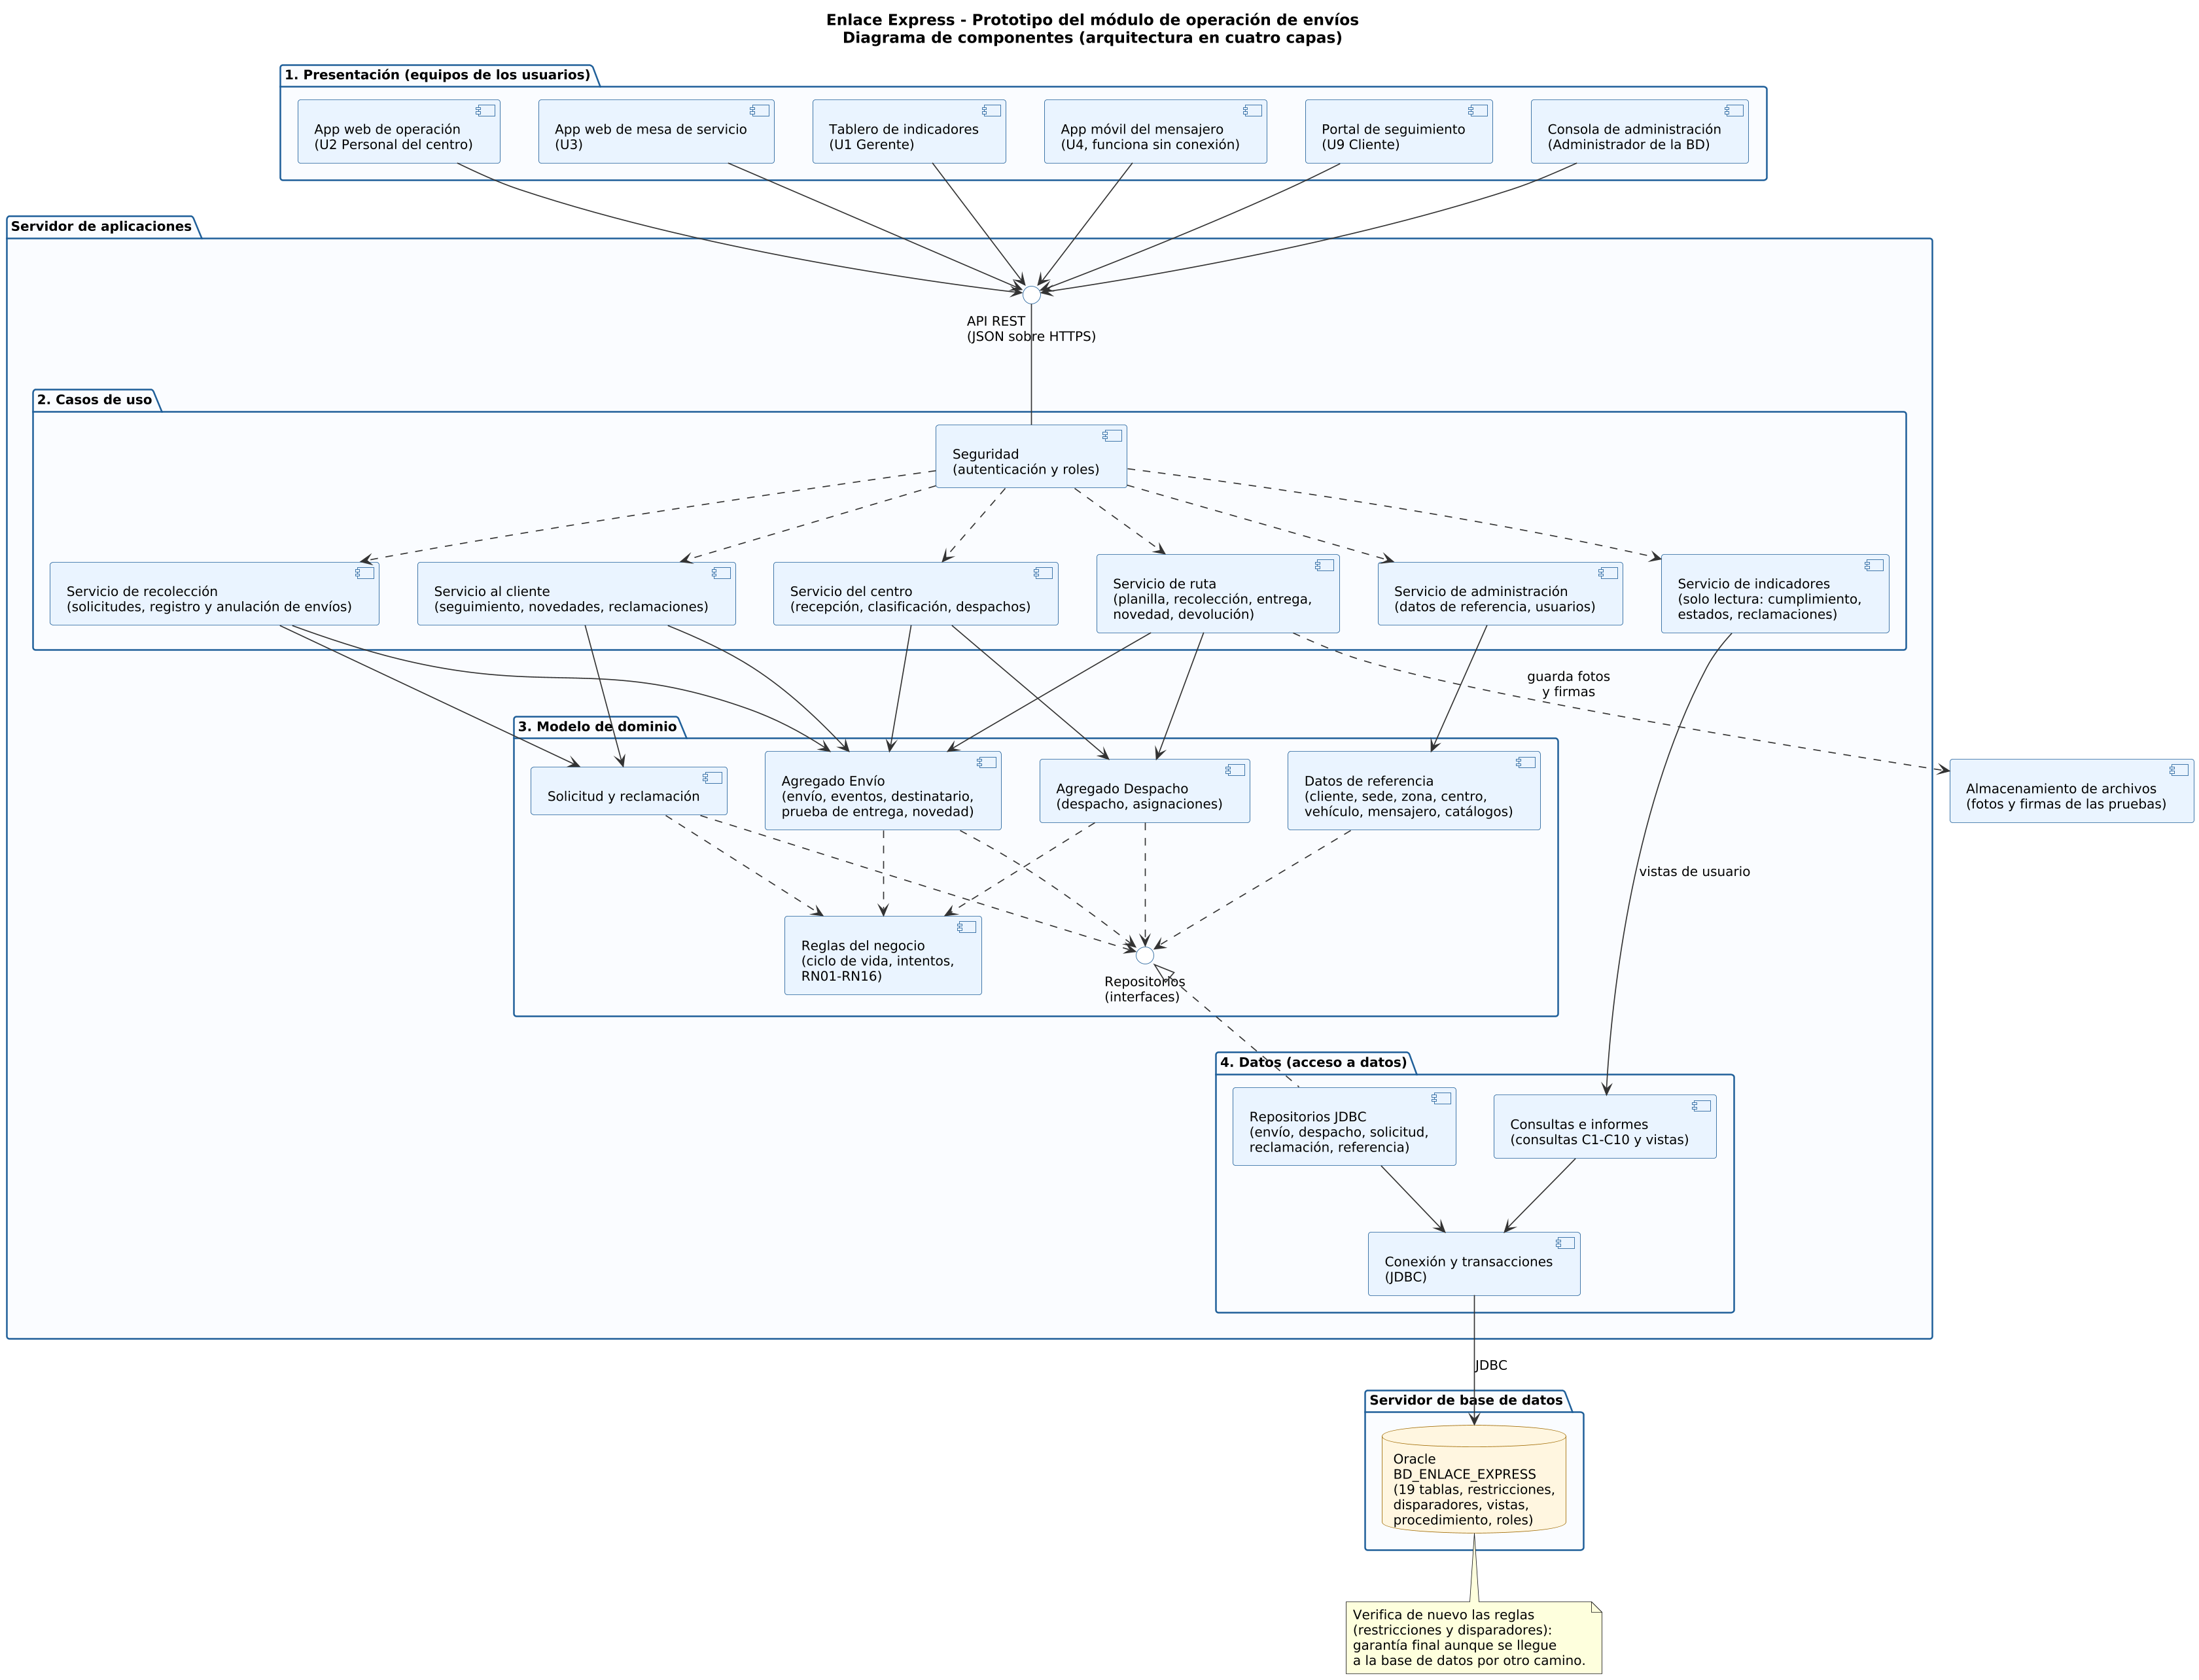
\includegraphics{figuras/prototipo/uml_componentes.png}}}
\caption{Diagrama de componentes del prototipo, en cuatro capas.}
\label{fig:proto-componentes}
\end{figure}

El diagrama de la figura~\ref{fig:proto-componentes} muestra la arquitectura
completa del diseño. El prototipo agrupa las aplicaciones de la capa de
presentación en una sola aplicación web con una sección por rol; no
implementa la aplicación móvil del mensajero con funcionamiento sin
conexión, la consola de administración ni el almacenamiento de fotos y
firmas, que están fuera del alcance (decisión A1).

\textbf{Casos de uso.} La figura~\ref{fig:proto-casos-uso-1} y la
figura~\ref{fig:proto-casos-uso-2} muestran el diagrama de casos de uso del
módulo, dividido en dos mitades para que se lea. La
tabla~\ref{tab:proto-cu} indica cuáles implementa el prototipo y cuál es
el servicio de la API de cada uno. Quedan fuera solo la gestión de datos de
referencia y de usuarios (CU27 y CU28), que la hace el administrador de la
base de datos con scripts, como dice el diseño, salvo el alta de cuentas de la
extensión E1. La gestión de novedades y de reclamaciones y la de centros y
zonas se probaron a nivel de base de datos en las transacciones T10 y T11
(subsección~\ref{sec:proto-transacciones}) y ahora también se hacen desde la
aplicación.

\begin{figure}[p]
\centering
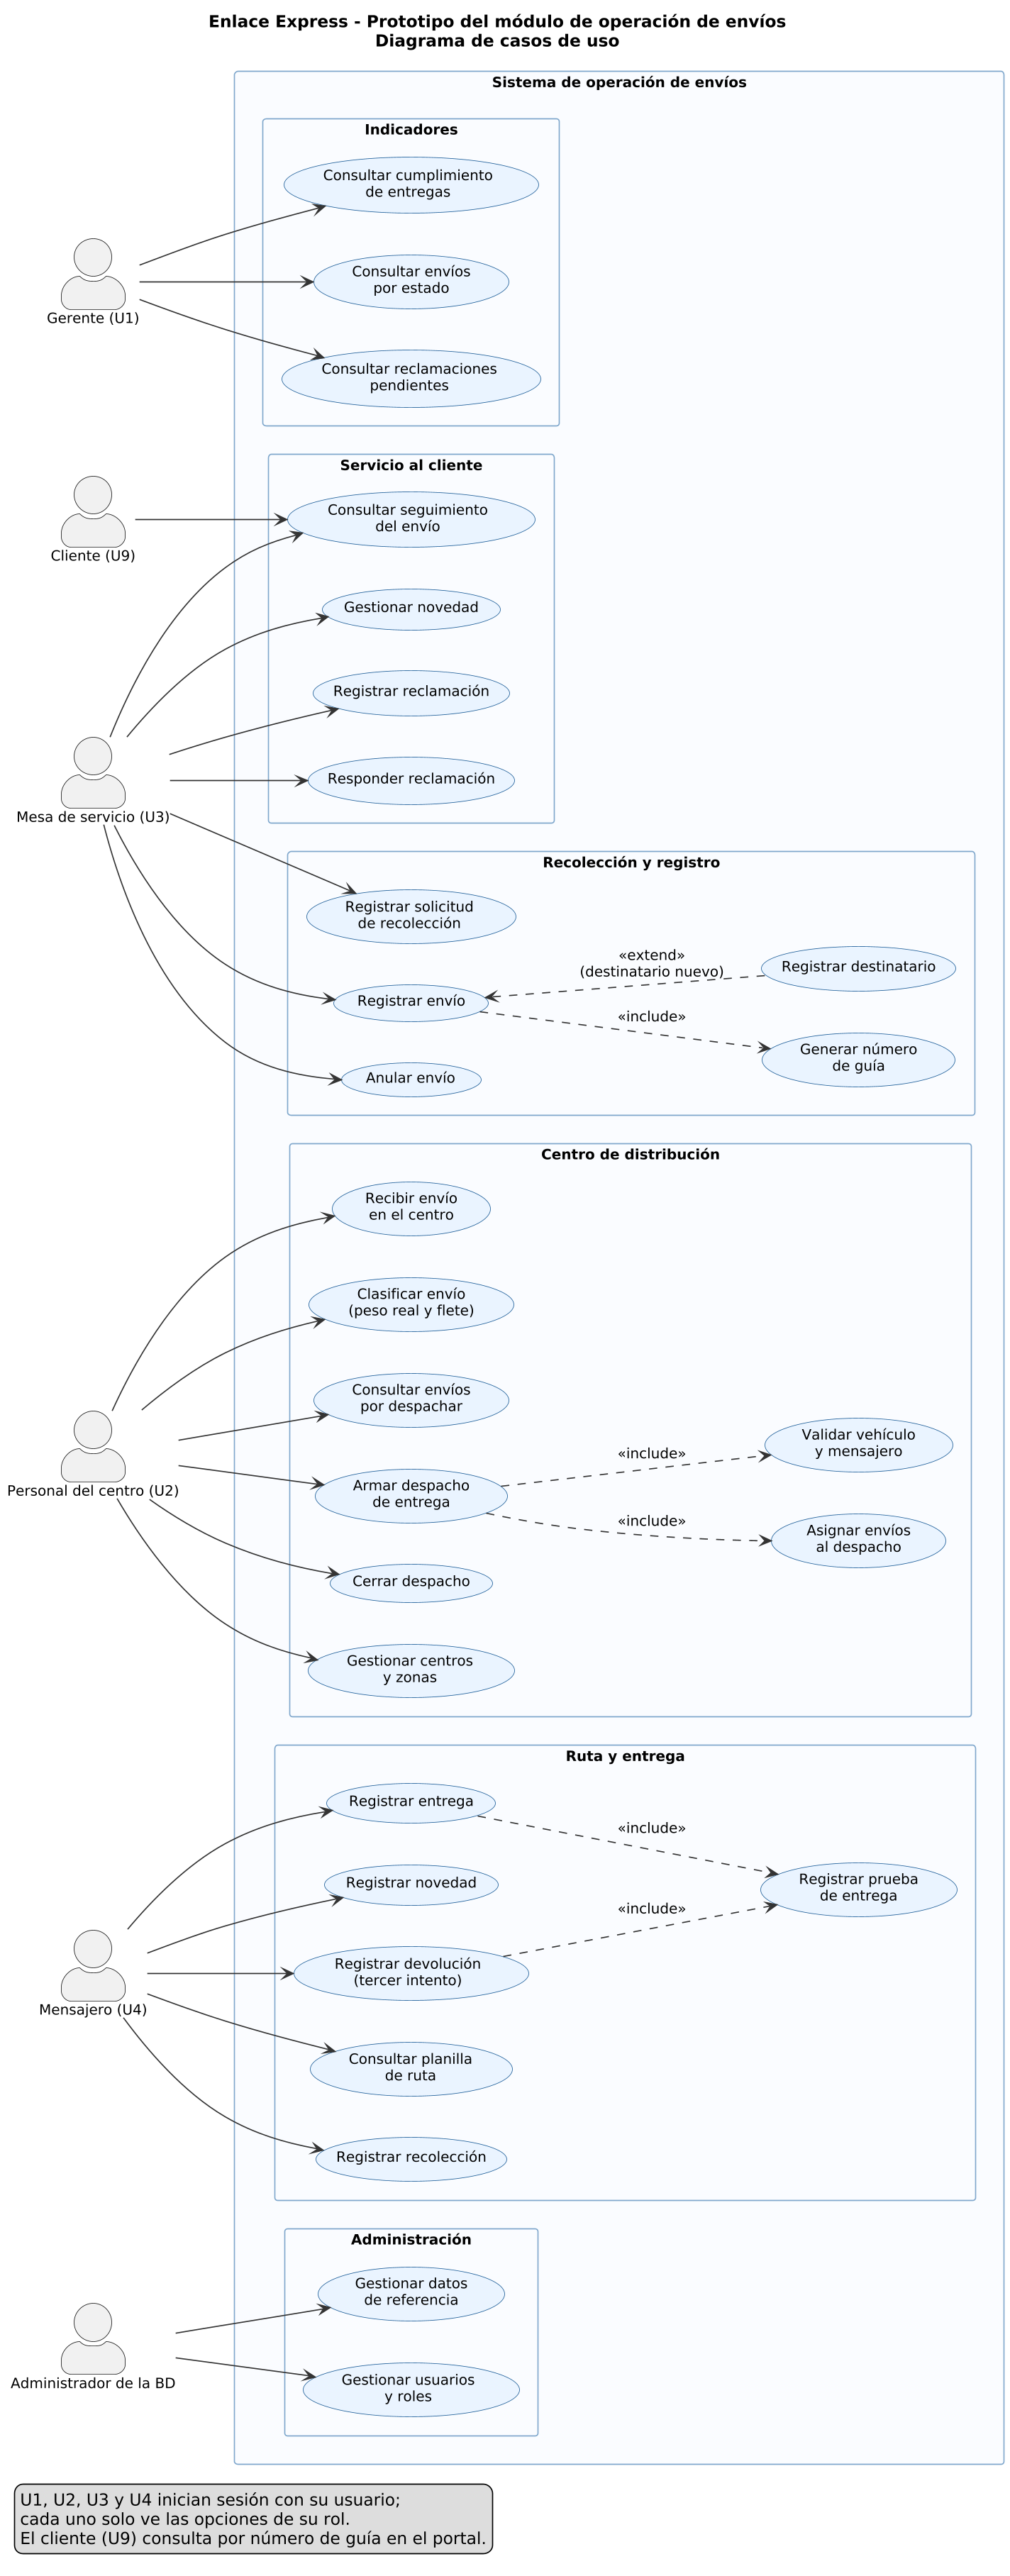
\includegraphics[trim=0 2023 0 0, clip, width=0.85\linewidth]{figuras/prototipo/uml_casos_uso.png}
\caption{Diagrama de casos de uso (primera parte): indicadores, servicio al cliente y recolección y registro.}
\label{fig:proto-casos-uso-1}
\end{figure}

\begin{figure}[p]
\centering
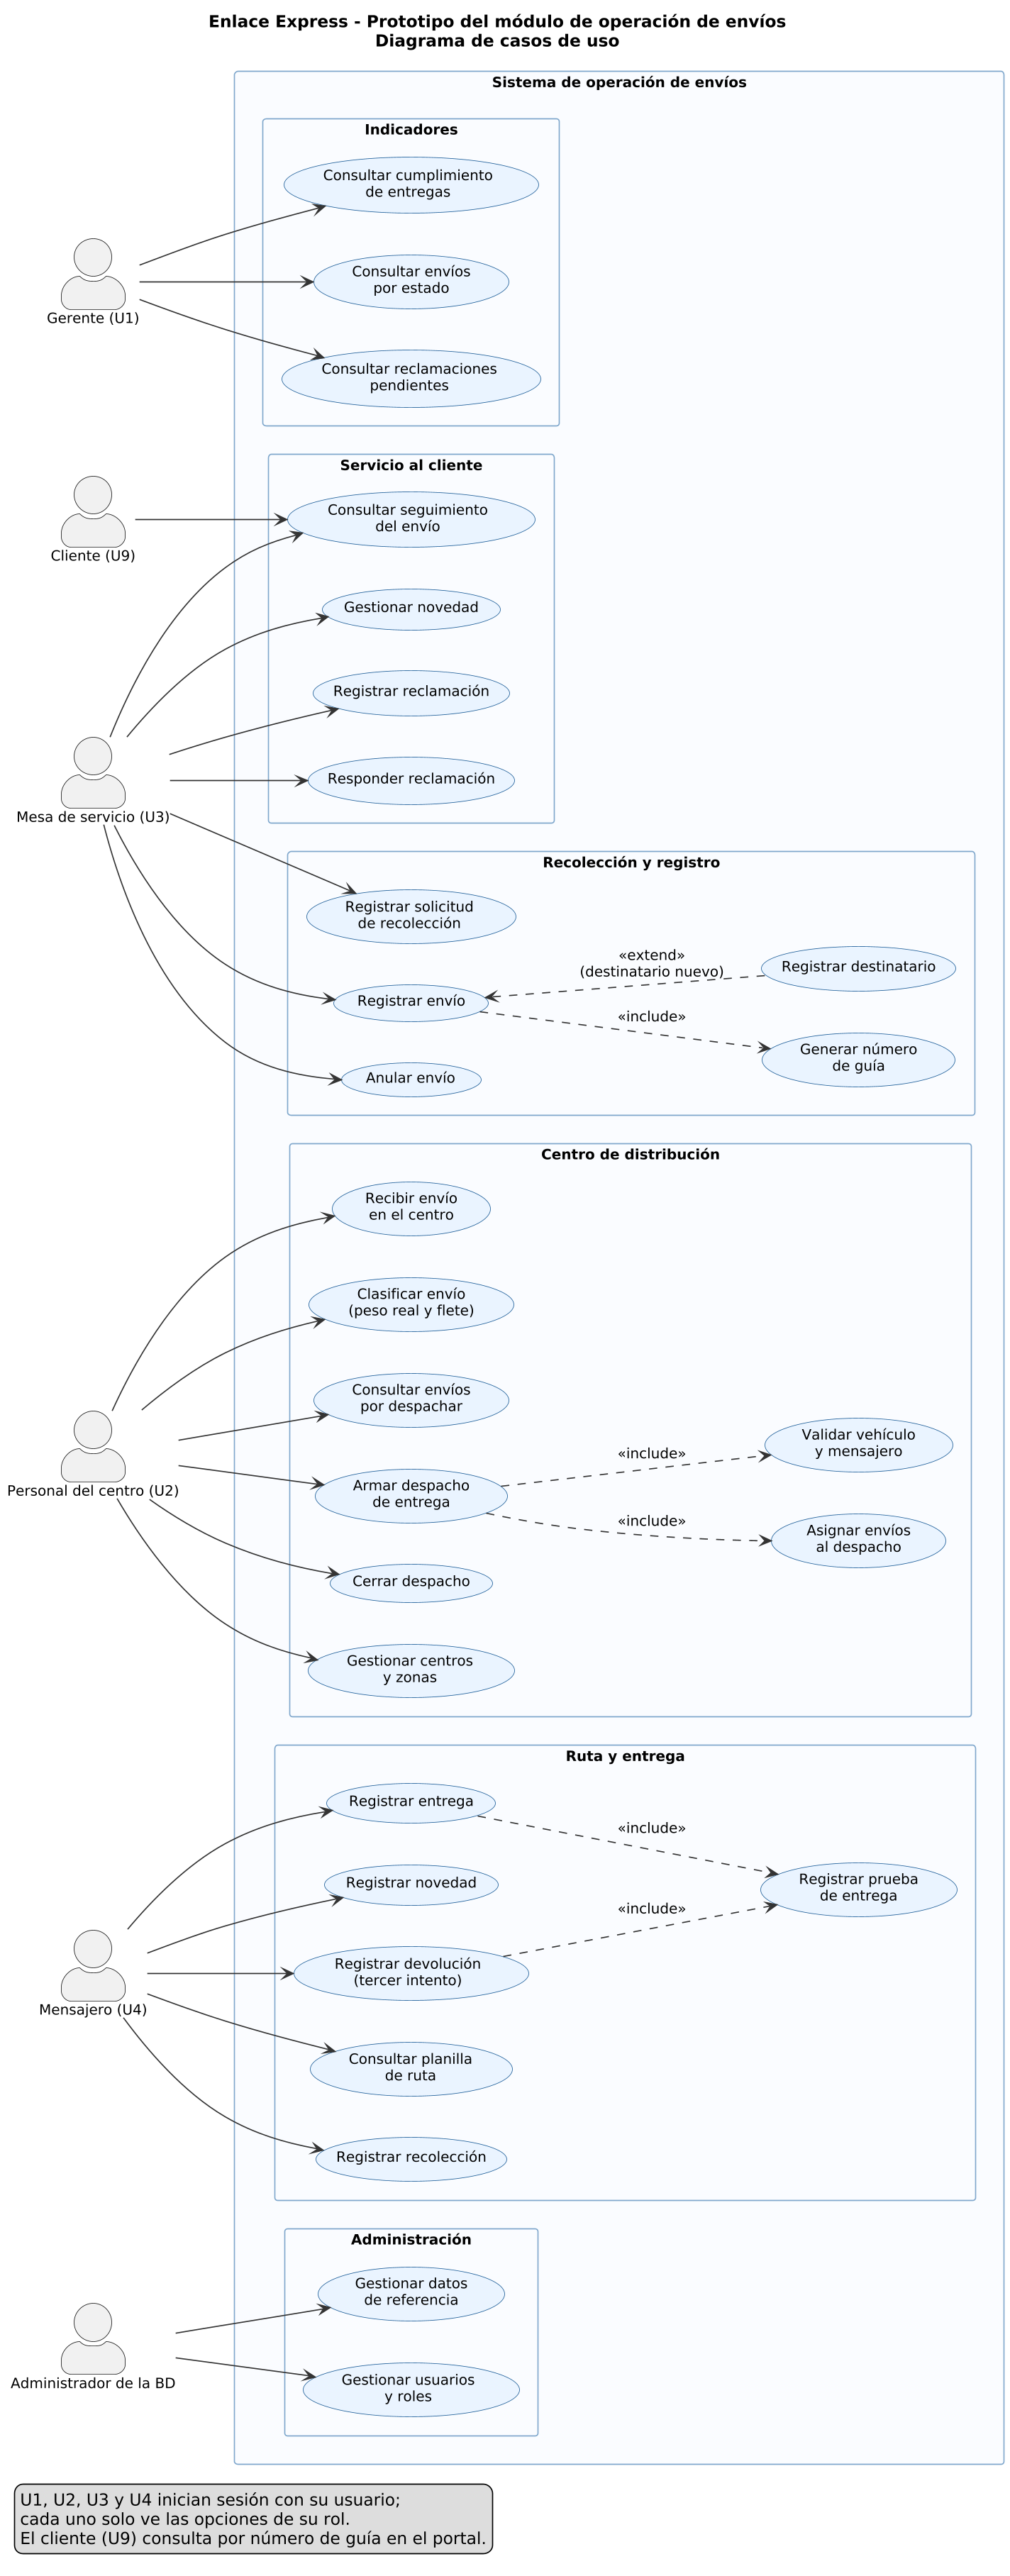
\includegraphics[trim=0 0 0 1609, clip, width=0.85\linewidth]{figuras/prototipo/uml_casos_uso.png}
\caption{Diagrama de casos de uso (segunda parte): centro de distribución, ruta y entrega, y administración.}
\label{fig:proto-casos-uso-2}
\end{figure}

{\singlespacing\footnotesize
\begin{longtable}{L{1.7cm} L{3.4cm} L{2.0cm} L{6.0cm}}
\caption{Casos de uso implementados por el prototipo y su servicio de la API.}
\label{tab:proto-cu}\\
\toprule
\textbf{Caso de uso} & \textbf{Nombre} & \textbf{Rol} & \textbf{Servicio de la API} \\
\midrule
\endfirsthead
\toprule
\textbf{Caso de uso} & \textbf{Nombre} & \textbf{Rol} & \textbf{Servicio de la API} \\
\midrule
\endhead
\bottomrule
\endfoot
CU01 & Registrar solicitud de recolección & Mesa & POST /api/\allowbreak{}mesa/\allowbreak{}solicitudes \\
CU02 a CU04 & Registrar envío (con número de guía y destinatario) & Mesa & POST /api/\allowbreak{}mesa/\allowbreak{}envios \\
CU05 & Anular envío & Mesa & POST /api/\allowbreak{}mesa/\allowbreak{}envios/\allowbreak{}\{guía\}/\allowbreak{}anular \\
CU06, CU07 & Recibir y clasificar envío & Centro & POST /api/\allowbreak{}centro/\allowbreak{}envios/\allowbreak{}\{guía\}/\allowbreak{}recepcion \\
CU08 & Consultar envíos por despachar & Centro & GET /api/\allowbreak{}centro/\allowbreak{}por-despachar \\
CU09 a CU11 & Armar despacho de entrega & Centro & POST /api/\allowbreak{}centro/\allowbreak{}despachos \\
CU12 & Cerrar despacho & Centro & POST /api/\allowbreak{}centro/\allowbreak{}despachos/\allowbreak{}\{id\}/\allowbreak{}cerrar \\
CU13 & Gestionar centros y zonas (sin borrar: el centro se inactiva) & Centro & GET y POST /api/\allowbreak{}centro/\allowbreak{}centros y /\allowbreak{}zonas; POST /api/\allowbreak{}centro/\allowbreak{}centros/\allowbreak{}\{id\}/\allowbreak{}modificar y /\allowbreak{}estado; POST /api/\allowbreak{}centro/\allowbreak{}zonas/\allowbreak{}\{id\}/\allowbreak{}modificar \\
CU14 & Consultar planilla de ruta & Mensajero, centro & GET /api/\allowbreak{}mensajero/\allowbreak{}planilla; GET /api/\allowbreak{}centro/\allowbreak{}despachos/\allowbreak{}\{id\}/\allowbreak{}planilla \\
CU15 & Registrar recolección & Mensajero & POST /api/\allowbreak{}mensajero/\allowbreak{}solicitudes/\allowbreak{}\{id\}/\allowbreak{}recolectar \\
CU16, CU19 & Registrar entrega con su prueba & Mensajero & POST /api/\allowbreak{}mensajero/\allowbreak{}asignaciones/\allowbreak{}\{id\}/\allowbreak{}entrega \\
CU17 & Registrar novedad & Mensajero & POST /api/\allowbreak{}mensajero/\allowbreak{}asignaciones/\allowbreak{}\{id\}/\allowbreak{}novedad \\
CU18 & Registrar devolución (tercer intento) & Mensajero & POST /api/\allowbreak{}mensajero/\allowbreak{}asignaciones/\allowbreak{}\{id\}/\allowbreak{}devolucion \\
CU20 & Consultar seguimiento del envío & Público, cliente, mesa & GET /api/\allowbreak{}publico/\allowbreak{}rastreo/\allowbreak{}\{guía\}; GET /api/\allowbreak{}cliente/\allowbreak{}envios/\allowbreak{}\{guía\}/\allowbreak{}seguimiento; GET /api/\allowbreak{}mesa/\allowbreak{}envios/\allowbreak{}\{guía\} \\
CU21 & Gestionar novedad (acción, solución y cierre) & Mesa & GET /api/\allowbreak{}mesa/\allowbreak{}novedades; POST /api/\allowbreak{}mesa/\allowbreak{}novedades/\allowbreak{}\{id\}/\allowbreak{}gestionar \\
CU22, CU23 & Registrar, responder y cerrar reclamaciones & Mesa & GET y POST /api/\allowbreak{}mesa/\allowbreak{}reclamaciones; POST /api/\allowbreak{}mesa/\allowbreak{}reclamaciones/\allowbreak{}\{id\}/\allowbreak{}responder y /\allowbreak{}cerrar \\
CU24 a CU26 & Consultar cumplimiento, envíos por estado y reclamaciones pendientes & Gerencia & GET /api/\allowbreak{}tablero/\allowbreak{}cumplimiento, /\allowbreak{}envios-por-estado y /\allowbreak{}reclamaciones-pendientes \\
\end{longtable}
\par}

La API está documentada con OpenAPI 3 y Swagger UI, que genera la
biblioteca springdoc a partir de los controladores: el documento se entrega
en \texttt{/v3/api-docs} y la interfaz en \texttt{/swagger-ui.html}, ambos sin
sesión y de solo lectura. Las rutas se agrupan por sección, cada una indica el
rol que exige, y el documento describe la sesión por cookie, el token CSRF y el
formato de los errores (Problem Details con la propiedad \texttt{codigo}). El
documento generado se guardó en \texttt{docs/evidence/13\_openapi.json} y una
captura de la interfaz en \texttt{docs/evidence/13\_swagger\_ui.png}.

\textbf{Dominio y acceso a datos.} Las figuras~\ref{fig:proto-clases-dominio}
y~\ref{fig:proto-clases-mapeadores} muestran las clases del modelo de dominio
y de los mapeadores. Los datos se leen y guardan con el patrón Data Mapper, sin
ORM: cada mapeador es una clase con el SQL de sus operaciones escrito como
constantes y ejecutado con \texttt{PreparedStatement} y variables de enlace.
Los valores nunca se concatenan en el SQL. El siguiente extracto de
\texttt{EnvioMapper} muestra el SQL que inserta un evento y el que bloquea la fila
de un envío, con el método que guarda el evento.

\begin{figure}[p]
\centering
\rotatebox{90}{\adjustbox{max width=0.95\textheight, max height=0.98\linewidth}{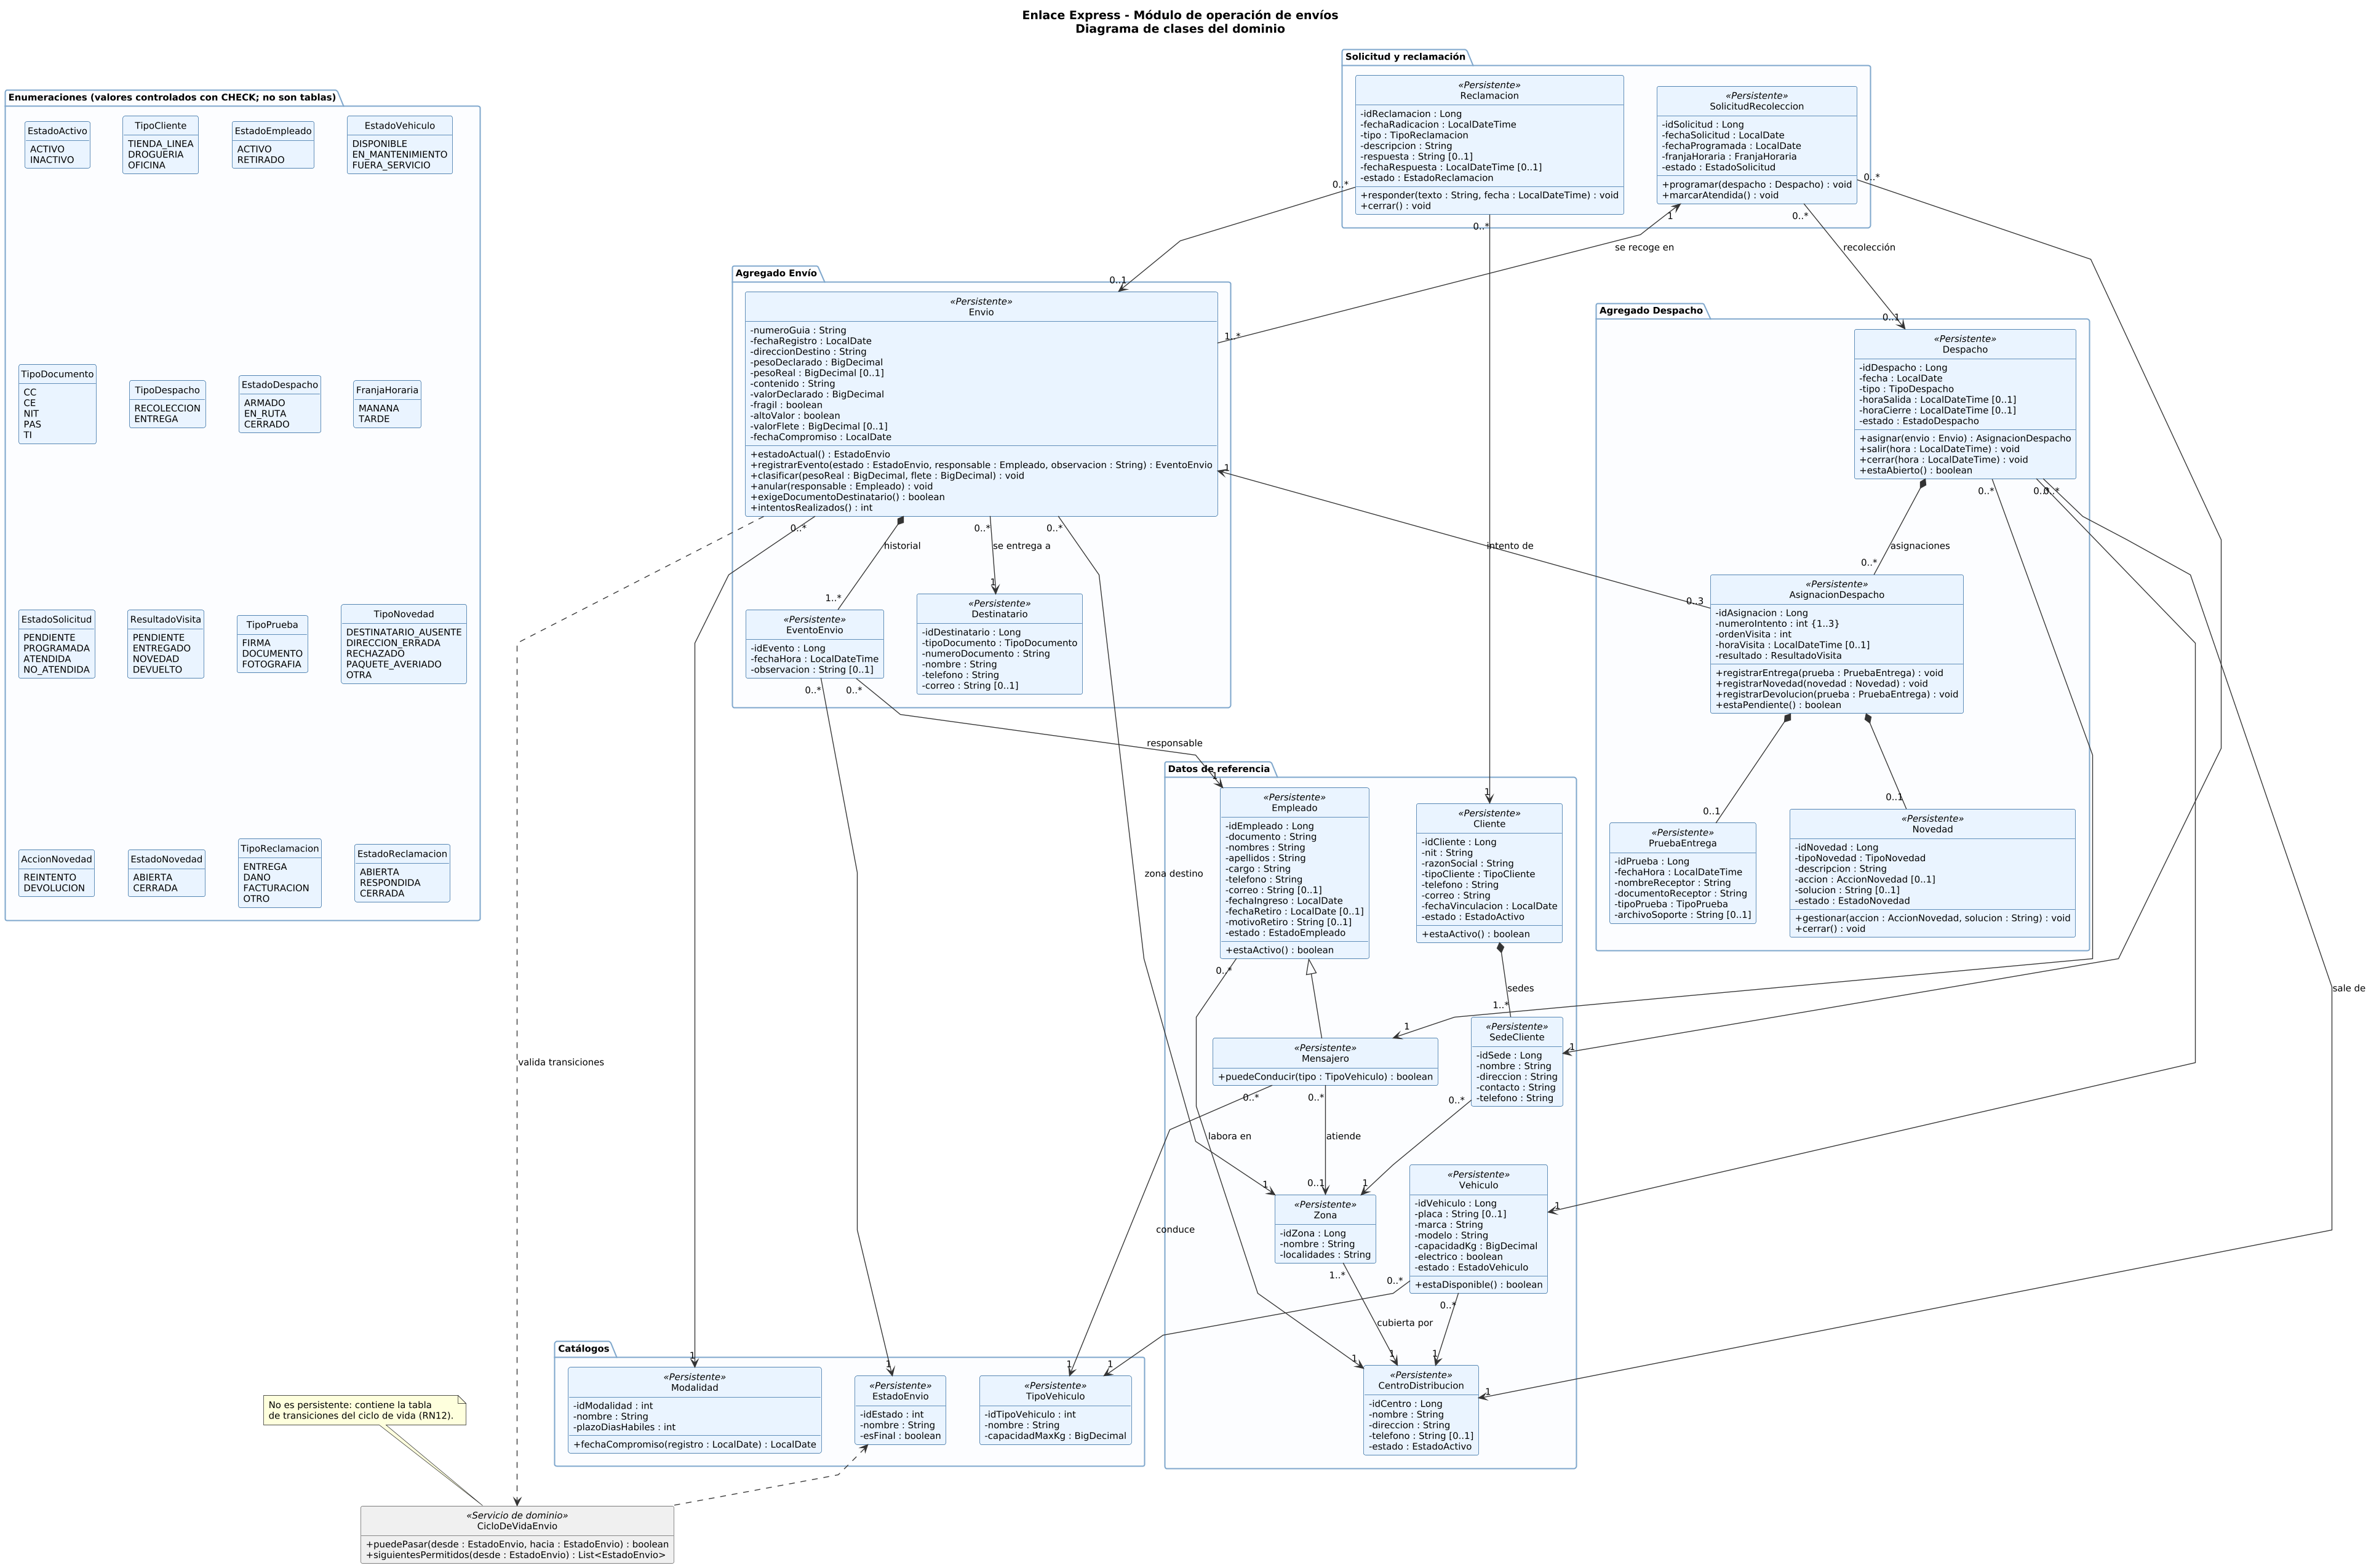
\includegraphics{figuras/prototipo/uml_clases_dominio.png}}}
\caption{Diagrama de clases del modelo de dominio.}
\label{fig:proto-clases-dominio}
\end{figure}

\begin{figure}[p]
\centering
\rotatebox{90}{\adjustbox{max width=0.95\textheight, max height=0.98\linewidth}{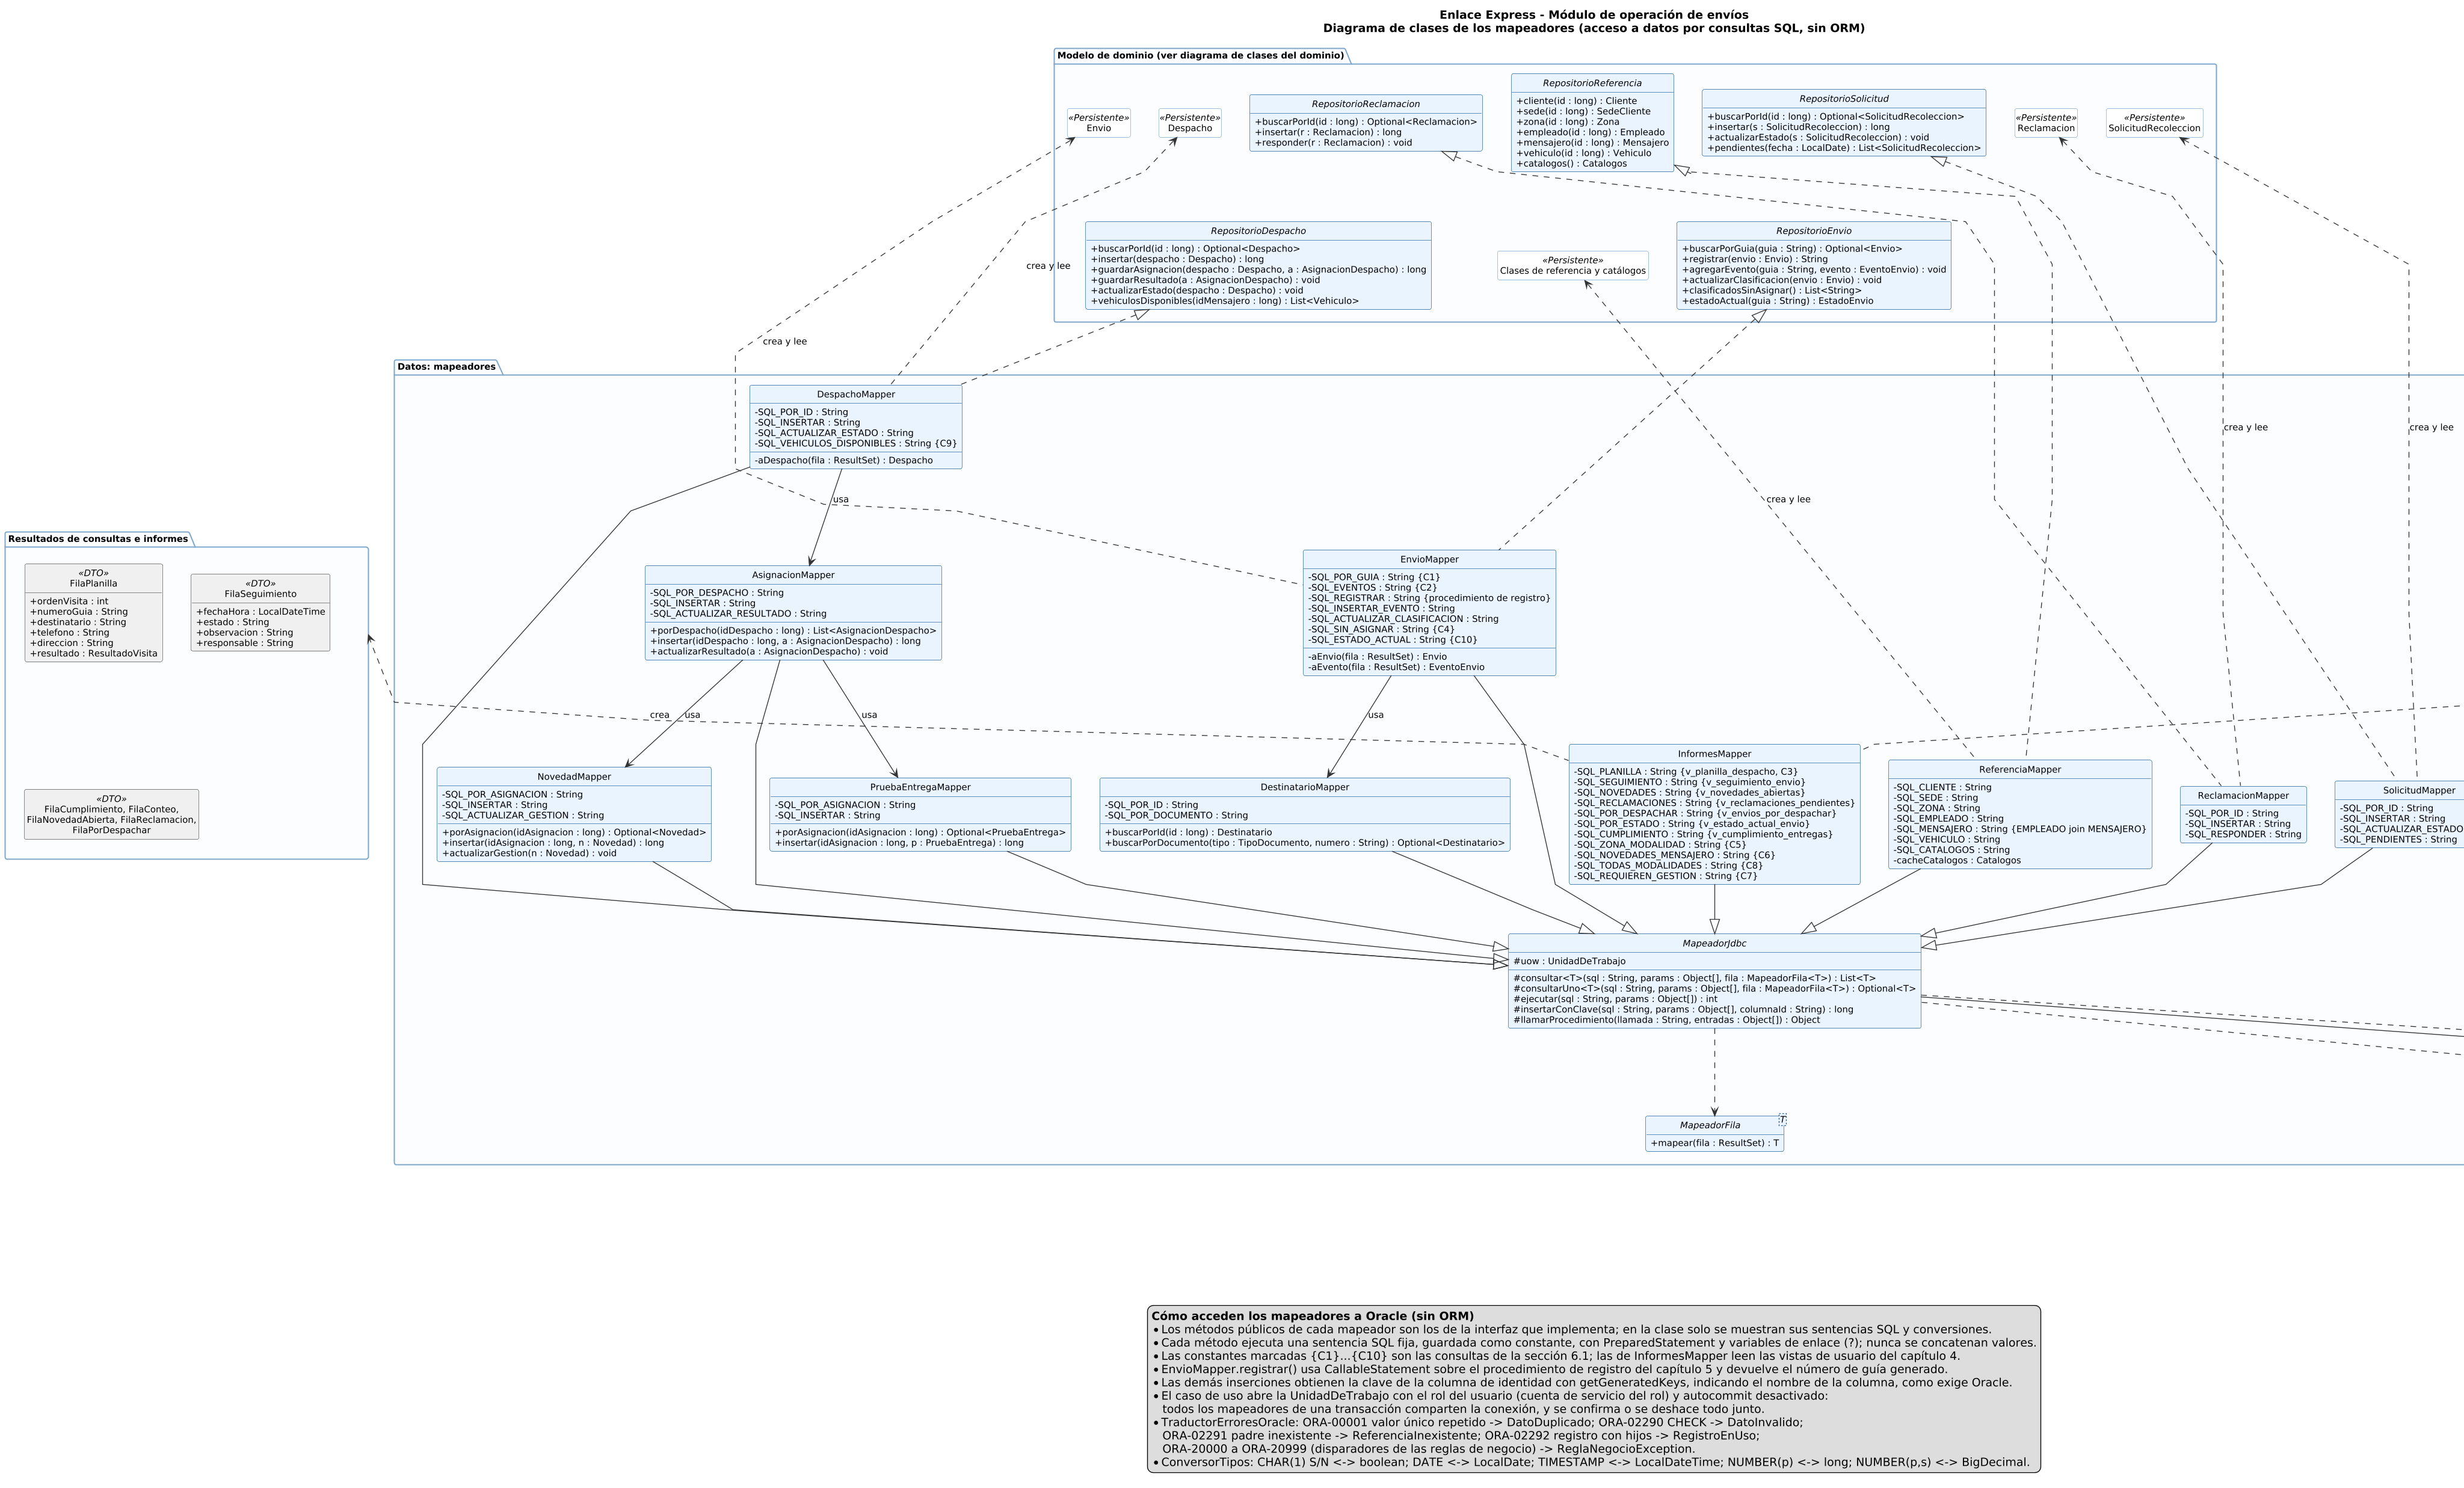
\includegraphics{figuras/prototipo/uml_clases_mapeadores.png}}}
\caption{Diagrama de clases de los mapeadores (Data Mapper sin ORM).}
\label{fig:proto-clases-mapeadores}
\end{figure}

% Los renglones del extracto se acomodaron para que quepan en la pagina.
\begin{lstlisting}[style=sqlpro,language=Java]
private static final String SQL_INSERTAR_EVENTO = """
    INSERT INTO evento_envio (numero_guia, id_estado,
           id_empleado, fecha_hora, observacion)
    VALUES (?, ?, ?, ?, ?)""";

private static final String SQL_BLOQUEAR =
    "SELECT numero_guia FROM envio WHERE numero_guia = ? FOR UPDATE";

public void agregarEvento(String numeroGuia, EventoEnvio evento) {
    long id = insertarConClave(SQL_INSERTAR_EVENTO,
        new Object[] {numeroGuia, evento.estado().idEstado(),
            evento.idEmpleado(), evento.fechaHora(),
            evento.observacion()}, "ID_EVENTO");
    evento.asignarId(id);
}
\end{lstlisting}

Tres clases de la infraestructura sostienen a los mapeadores:

\begin{itemize}[itemsep=2pt]
  \item \textbf{\texttt{UnidadDeTrabajo}} es una transacción: una conexión de
        la cuenta de servicio del rol, sin confirmación automática, que
        comparten todos los mapeadores de un caso de uso. Se confirma o se
        deshace todo junto, sin \texttt{@Transactional}: el caso de uso la
        abre al empezar, llama a \texttt{confirmar} al final y, si
        falla antes, al cerrarla se deshace sola.
  \item \textbf{\texttt{FabricaConexiones}} mantiene un pequeño grupo de
        conexiones por cuenta de servicio, una por rol. Cada conexión nueva
        fija el esquema BD\_ENLACE\_EXPRESS y la zona horaria America/Bogota,
        de modo que el SQL es el mismo de la sección~\ref{sec:algebra}.
  \item \textbf{\texttt{TraductorErroresOracle}} convierte los errores de
        Oracle en excepciones del dominio, que la API responde con un código HTTP
        y el formato de errores estándar Problem Details, con la propiedad
        \texttt{codigo}. La tabla~\ref{tab:proto-errores} resume la
        conversión.
\end{itemize}

{\singlespacing\small
\begin{longtable}{L{4.8cm} L{1.4cm} L{5.4cm}}
\caption{Conversión de errores de Oracle a respuestas de la API.}
\label{tab:proto-errores}\\
\toprule
\textbf{Error de Oracle} & \textbf{HTTP} & \textbf{Código de la respuesta} \\
\midrule
\endfirsthead
\toprule
\textbf{Error de Oracle} & \textbf{HTTP} & \textbf{Código de la respuesta} \\
\midrule
\endhead
\bottomrule
\endfoot
ORA-20000 a ORA-20999 (reglas de negocio y E1) & 422 & El de la regla: RN07, E1, etc. \\
ORA-02290, ORA-01400, ORA-12899 (CHECK, NOT NULL, longitud) & 400 & DATO\_INVALIDO \\
ORA-02291 (clave foránea inexistente) & 400 & REFERENCIA\_INEXISTENTE \\
ORA-00001 (UNIQUE) & 409 & DATO\_DUPLICADO \\
ORA-02292 (registro con dependientes) & 409 & REGISTRO\_EN\_USO \\
ORA-00054 (recurso ocupado) & 409 & RECURSO\_OCUPADO \\
ORA-00942, ORA-01031, ORA-41900 (privilegio) & 403 & ACCESO\_DENEGADO \\
Cualquier otro & 500 & ERROR\_INTERNO, sin detalles de la base \\
\end{longtable}
\par}

\textbf{Reglas en dos niveles.} Las reglas de negocio se verifican primero en el
dominio, con el mismo código y el mismo texto que usa Oracle, y la base de
datos las vuelve a verificar como garantía final. La regla RN12 muestra los
dos niveles. En el dominio, \texttt{CicloDeVidaEnvio} rechaza una
transición no permitida con el código RN12 y la prueba unitaria
\texttt{CicloDeVidaEnvioTest} lo comprueba. En la base de datos, el disparador
\texttt{trg\_evento\_transicion} rechaza la misma transición con ORA-20012,
que probaron las transacciones (T3 a T7 y T12,
tabla~\ref{tab:proto-casos}). Para el usuario, ambos dan el mensaje que
aparece en la figura~\ref{fig:proto-rn12}, que empieza por el código de la
regla.

\textbf{Seguridad.} El acceso sigue tres pasos: el rol de la aplicación del
usuario que inició sesión decide qué servicios puede llamar; el servidor elige
entonces la cuenta de servicio de ese rol; y la base de datos limita lo que esa
cuenta puede hacer con los permisos del capítulo~5.

\begin{itemize}[itemsep=2pt]
  \item \textbf{Sesión y contraseñas.} La sesión vive en el servidor y el
        navegador solo guarda una cookie, protegida contra el acceso desde
        scripts y con la restricción \texttt{SameSite}. Las contraseñas se
        guardan con BCrypt. Una contraseña débil o un dato faltante se
        rechazan, y un usuario o una contraseña incorrectos dan siempre el
        mismo mensaje.
  \item \textbf{CSRF.} Las operaciones que cambian datos exigen un
        token contra falsificación de peticiones (CSRF), que el navegador
        devuelve en un encabezado.
  \item \textbf{Registro con código (E1).} Un empleado o un cliente se
        registra con su documento o NIT y un código de activación de un solo
        uso, y el rol lo deriva la base de datos del cargo
        (subsección~\ref{sec:proto-extensiones}).
  \item \textbf{Identificador de cliente.} Cada transacción fija, con el
        nombre del usuario, el identificador de cliente de la sesión de Oracle
        (decisión A2). El script
        \texttt{test-client-\allowbreak identifier.sh} lo comprobó
        con la auditoría unificada de Oracle: \texttt{demo\_mesa} registró una
        solicitud y un envío por la API, y la auditoría guardó su nombre como
        identificador de cliente aunque la conexión es de la cuenta
        \texttt{svc\_mesa} (tabla~\ref{tab:proto-auditoria}).
  \item \textbf{Rastreo público (E2).} Cualquiera consulta un envío por su
        número de guía, sin cuenta, y ve solo fecha, estado y zona de cada
        evento. La aplicación limita las consultas por dirección IP, y la
        prueba de integración \texttt{SeguridadIT} comprueba que la consulta
        número 31 dentro de un minuto recibe el estado 429.
\end{itemize}

% Fuente: docs/evidence/11_identificador_cliente.txt
{\singlespacing\small
\begin{longtable}{L{2.8cm} L{2.2cm} L{2.8cm} L{2.2cm} L{3.6cm}}
\caption{Auditoría de Oracle de una operación hecha por la aplicación con el usuario demo\_mesa.}
\label{tab:proto-auditoria}\\
\toprule
\textbf{Hora} & \textbf{Cuenta de la base} & \textbf{Identificador de cliente} & \textbf{Acción} & \textbf{Objeto} \\
\midrule
\endfirsthead
\toprule
\textbf{Hora} & \textbf{Cuenta de la base} & \textbf{Identificador de cliente} & \textbf{Acción} & \textbf{Objeto} \\
\midrule
\endhead
\bottomrule
\endfoot
21/11/2026 16:55:31 & SVC\_MESA & demo\_mesa & INSERT & SOLICITUD\_\allowbreak RECOLECCION \\
21/11/2026 16:55:31 & SVC\_MESA & demo\_mesa & EXECUTE & PR\_REGISTRAR\_\allowbreak ENVIO \\
\end{longtable}
\par}

\textbf{Flujo principal.} El flujo principal definido para el prototipo es: registrar
el envío, recolectarlo, recibirlo y clasificarlo, armar el despacho,
entregar con prueba y consultar el seguimiento público; después, un caso
de rechazo con la devolución en el tercer intento y una transición bloqueada.
La prueba de punta a punta, que se describe al final de esta subsección,
lo recorre en el navegador con los usuarios de demostración y guardó una
captura de cada paso; las que siguen son las principales. Los envíos del
recorrido son EE0000000000030, el frágil, y EE0000000000031, el que termina
devuelto.

El rastreo público (figura~\ref{fig:proto-rastreo}) es la pantalla de inicio y
no pide sesión: muestra el estado actual y la línea de tiempo del envío.

\begin{figure}[htbp]
\centering
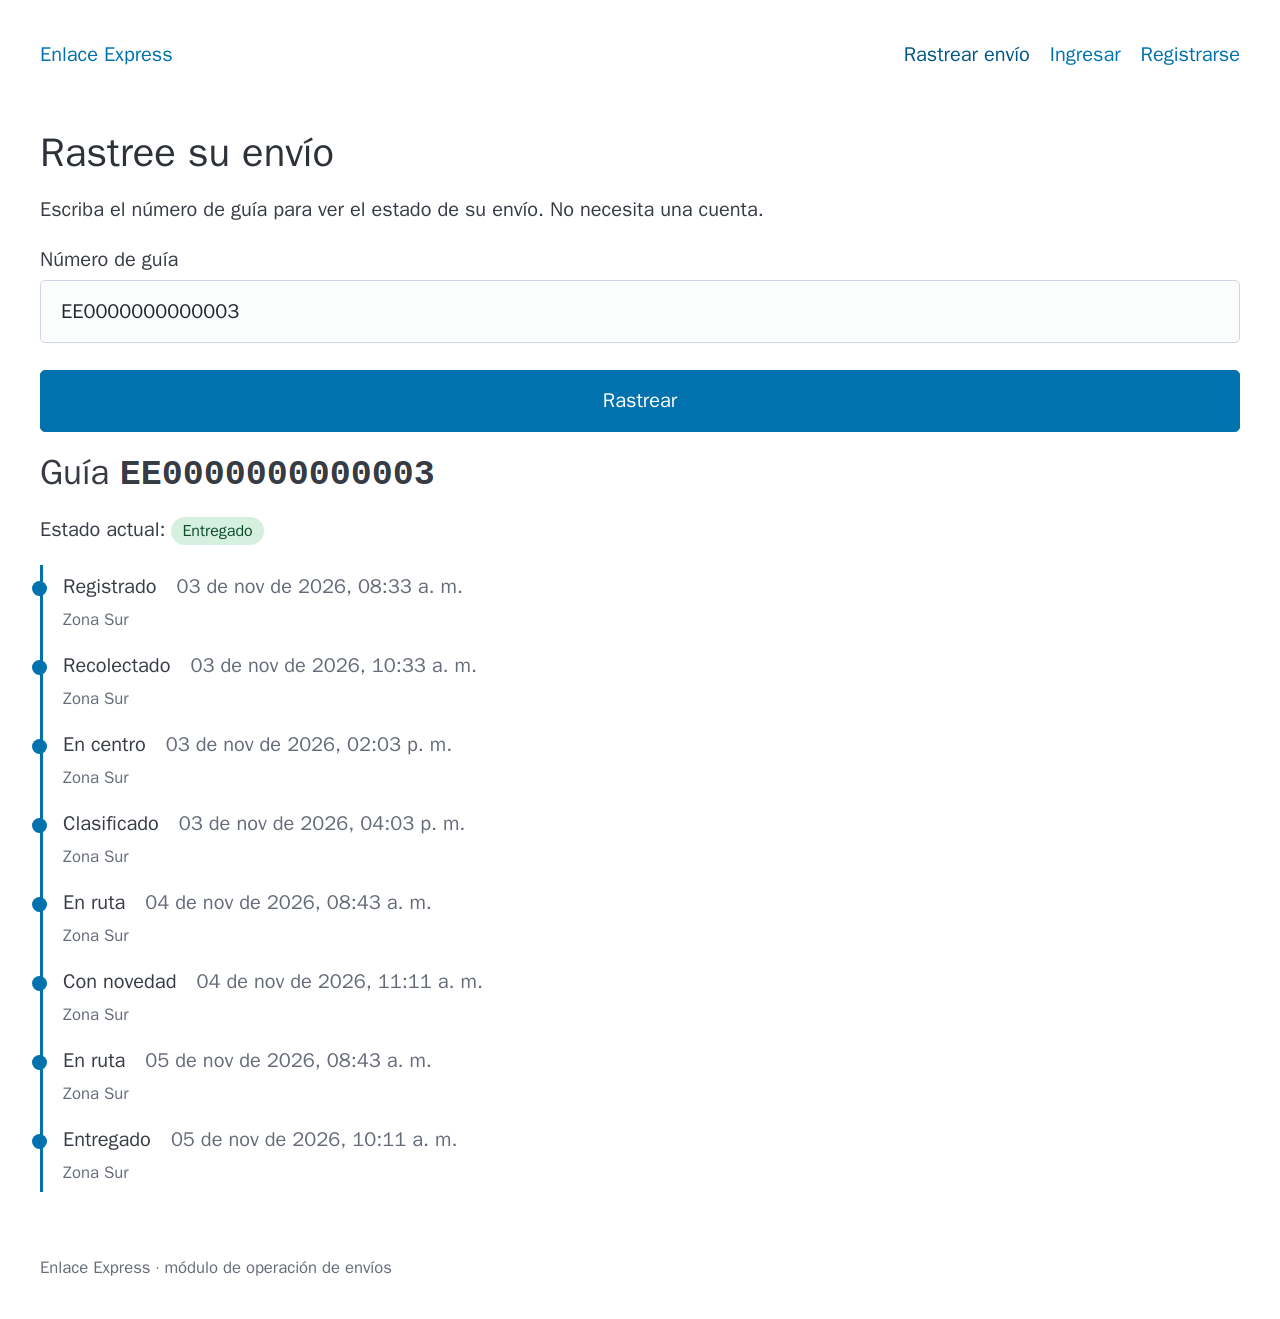
\includegraphics[width=0.6\linewidth]{figuras/prototipo/01_rastreo_publico.png}
\caption{Rastreo público de la guía EE0000000000003: estado actual y recorrido con fecha, estado y zona, sin datos personales.}
\label{fig:proto-rastreo}
\end{figure}

La mesa de servicio, después de iniciar sesión, registra la solicitud de
recolección del cliente y luego los envíos, uno frágil y uno normal. Al
registrar un envío, la aplicación muestra el número de guía que genera
la base de datos y la fecha de compromiso que calcula con la modalidad
(figura~\ref{fig:proto-registro}).

\begin{figure}[htbp]
\centering
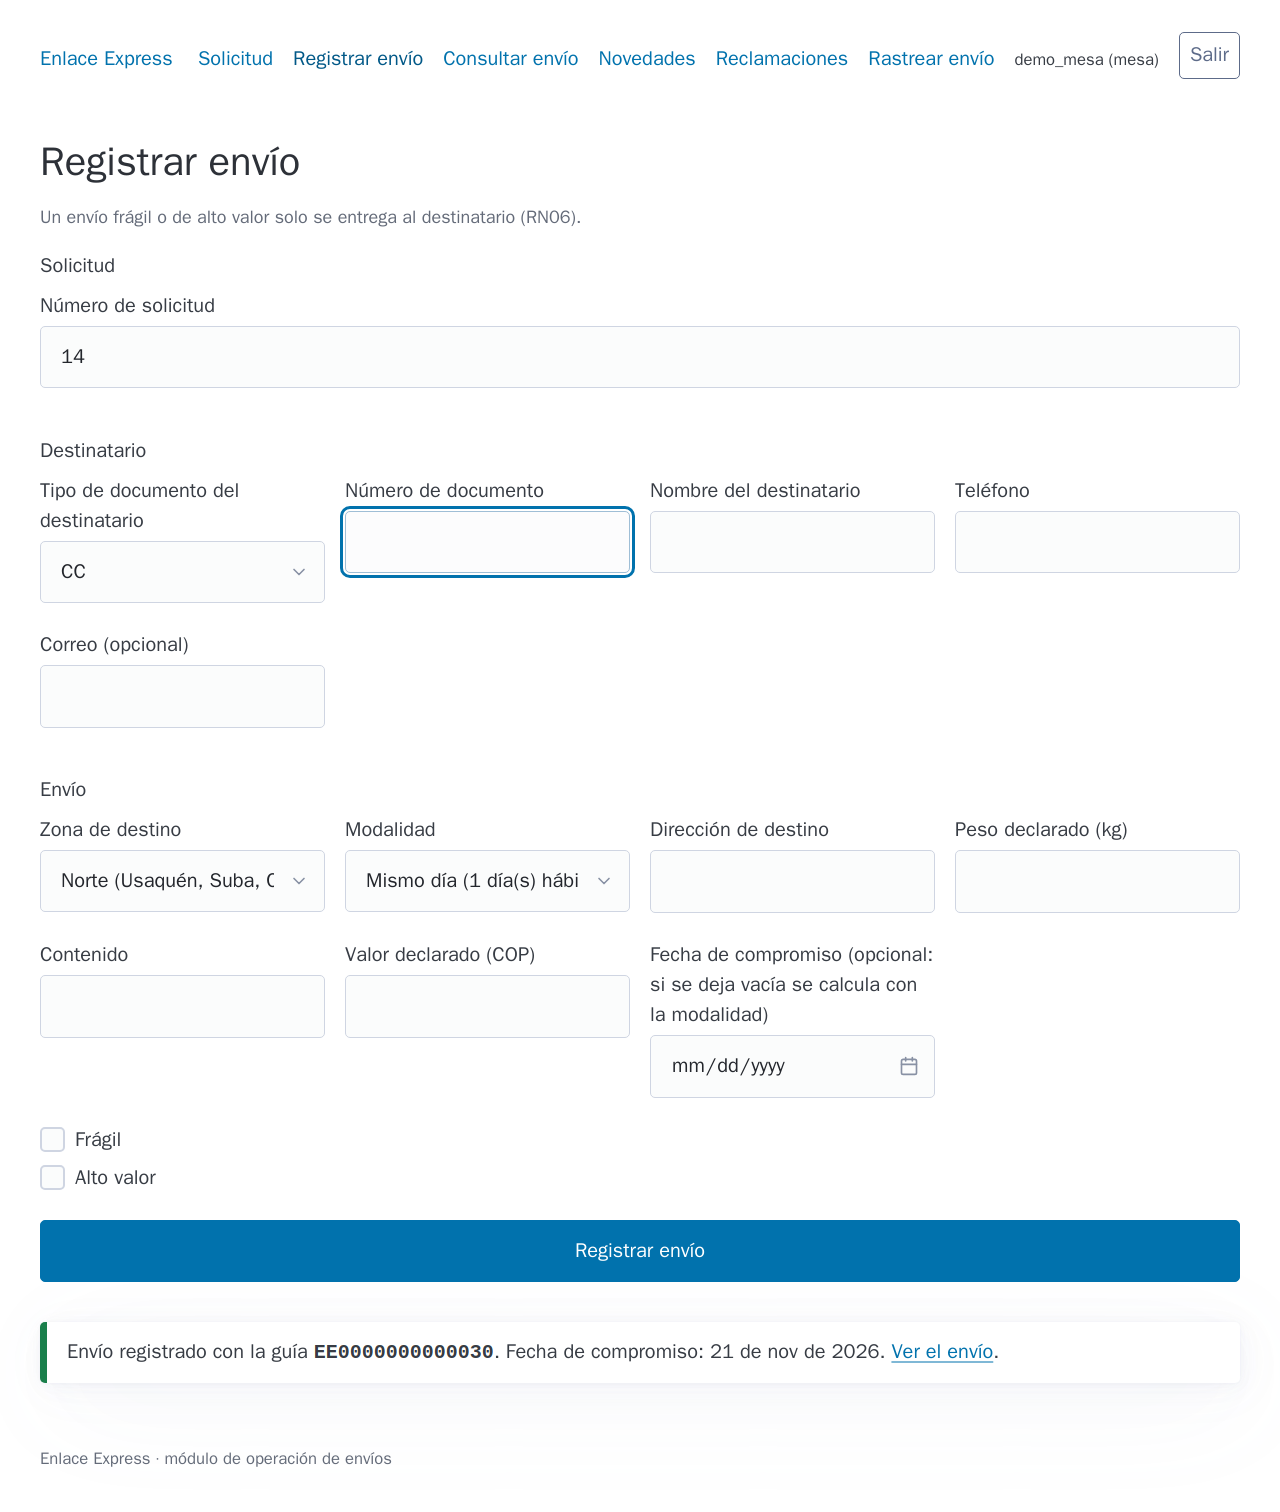
\includegraphics[trim=0 70 0 0, clip, width=0.6\linewidth]{figuras/prototipo/04_mesa_registro_envio.png}
\caption{Registro de un envío por la mesa de servicio: el mensaje de éxito muestra la guía y la fecha de compromiso.}
\label{fig:proto-registro}
\end{figure}

El mensajero recolecta la solicitud, y el centro recibe cada envío con su peso
real y su flete (figura~\ref{fig:proto-recepcion}), que quedan clasificados. Luego
el centro arma el despacho de entrega: elige los envíos clasificados, un
mensajero y uno de los vehículos disponibles de su tipo, y la aplicación
informa el número de despacho (figura~\ref{fig:proto-despacho}).

\begin{figure}[htbp]
\centering
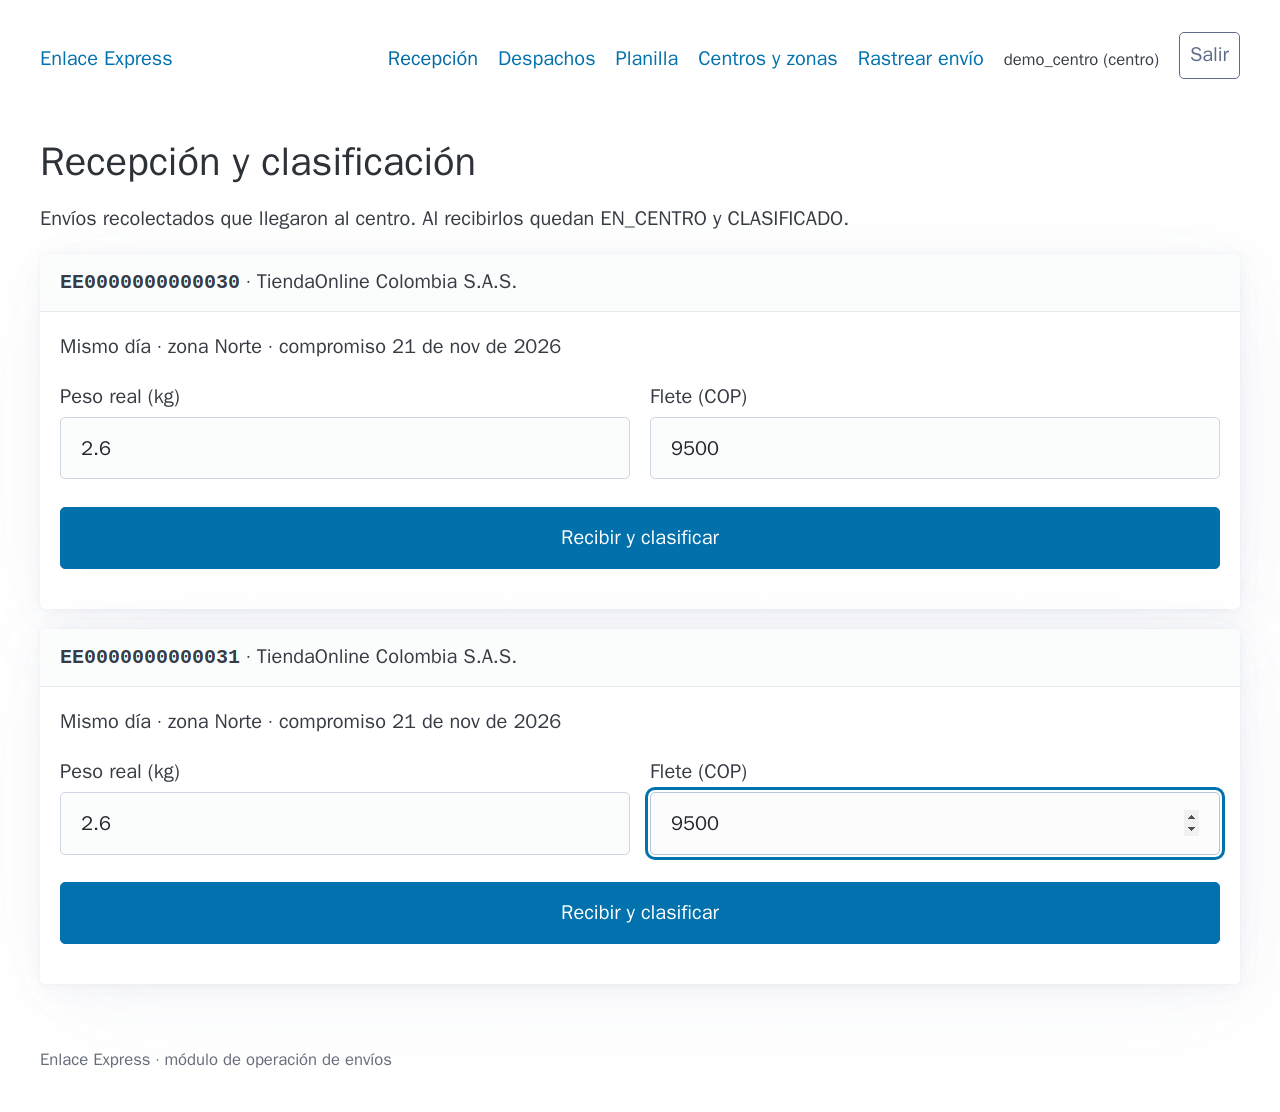
\includegraphics[width=0.75\linewidth]{figuras/prototipo/06_centro_recepcion.png}
\caption{Recepción y clasificación en el centro: peso real y flete de cada envío recolectado.}
\label{fig:proto-recepcion}
\end{figure}

\begin{figure}[htbp]
\centering
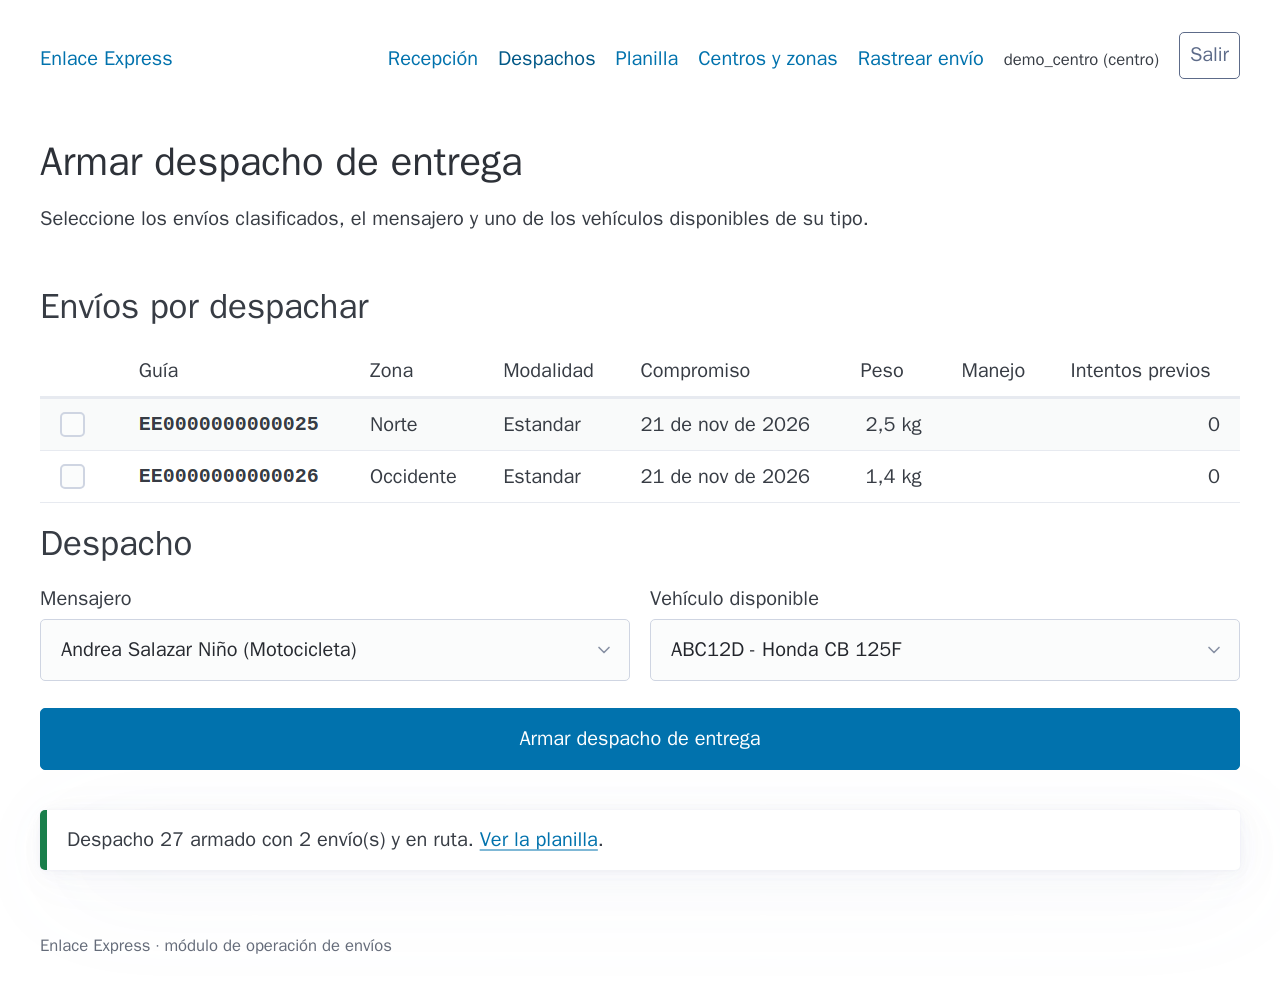
\includegraphics[width=0.75\linewidth]{figuras/prototipo/07_centro_despacho_armado.png}
\caption{Despacho armado por el centro, con el aviso del número de despacho.}
\label{fig:proto-despacho}
\end{figure}

La planilla del mensajero se diseñó para el teléfono: una columna, botones
grandes y el envío frágil resaltado, con la indicación de que solo se
entrega al destinatario. En la figura~\ref{fig:proto-movil} el mensajero intenta
entregar el envío frágil con el documento de otra persona y el sistema rechaza la
entrega con el mensaje de la regla RN06; con el documento del destinatario
la entrega se acepta.

\begin{figure}[htbp]
\centering
\begin{minipage}[t]{0.40\linewidth}
\centering
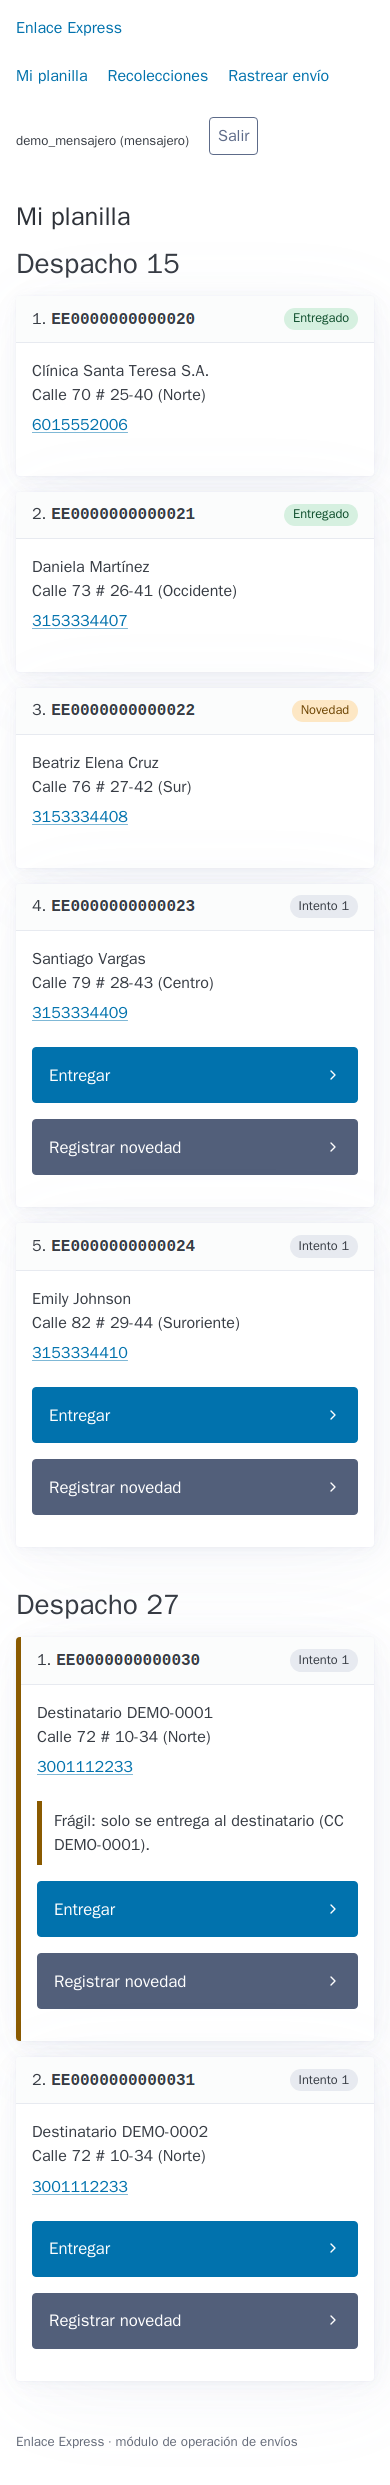
\includegraphics[trim=0 385 0 1560, clip, width=\linewidth]{figuras/prototipo/09_mensajero_planilla_movil.png}
\end{minipage}\hfill
\begin{minipage}[t]{0.40\linewidth}
\centering
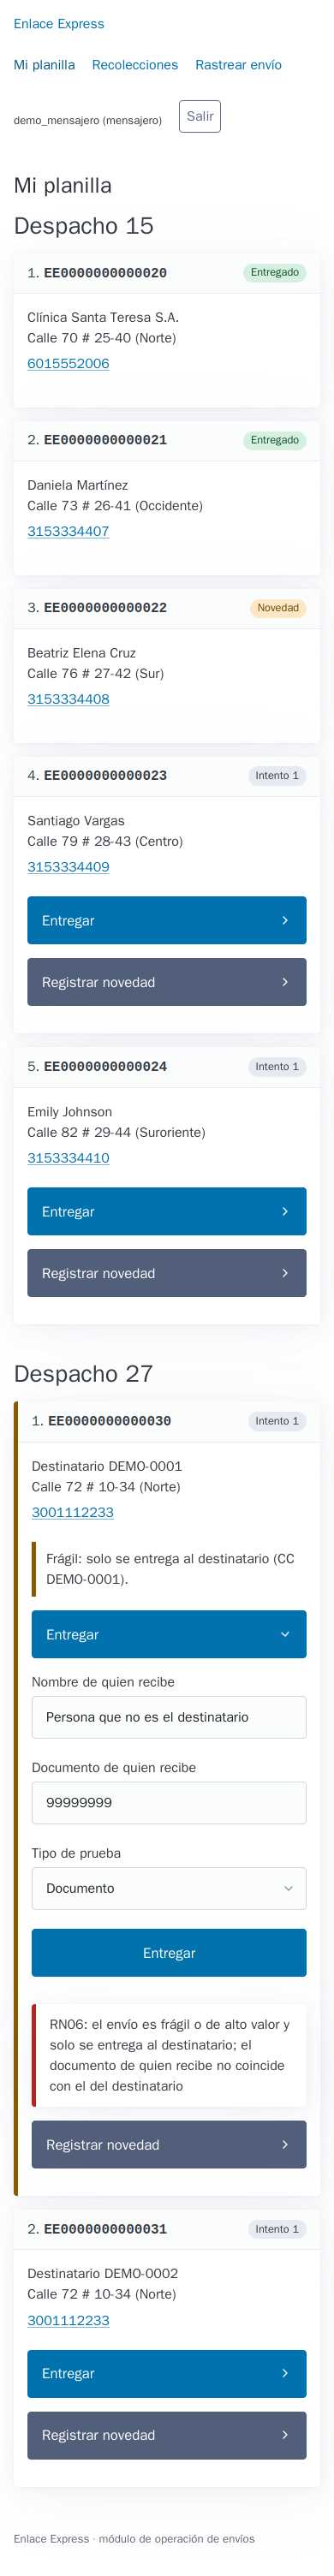
\includegraphics[trim=0 409 0 1590, clip, width=\linewidth]{figuras/prototipo/10_rechazo_rn06_movil.png}
\end{minipage}
\caption{Planilla del mensajero en el teléfono, con el envío frágil resaltado (izquierda), y rechazo RN06 al intentar entregarlo con el documento de otra persona (derecha).}
\label{fig:proto-movil}
\end{figure}

El cliente ve sus envíos y el recorrido completo de cada uno
(figura~\ref{fig:proto-cliente}), y la gerencia ve el tablero con el
cumplimiento por zona y los envíos por estado y, más abajo, las
reclamaciones pendientes (figura~\ref{fig:proto-tablero}).

\begin{figure}[htbp]
\centering
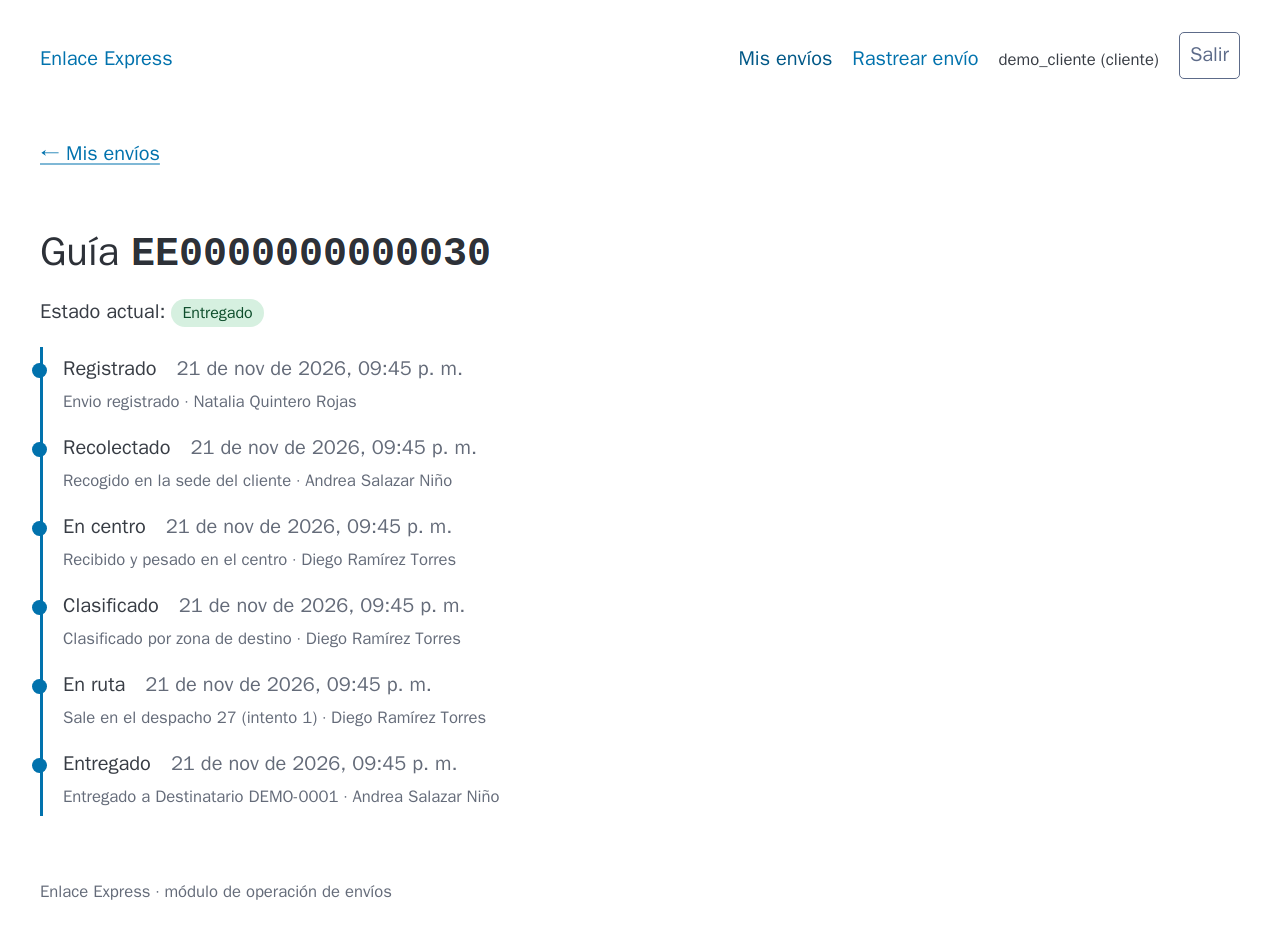
\includegraphics[width=0.75\linewidth]{figuras/prototipo/15_cliente_recorrido.png}
\caption{Recorrido de un envío entregado en el portal del cliente.}
\label{fig:proto-cliente}
\end{figure}

\begin{figure}[htbp]
\centering
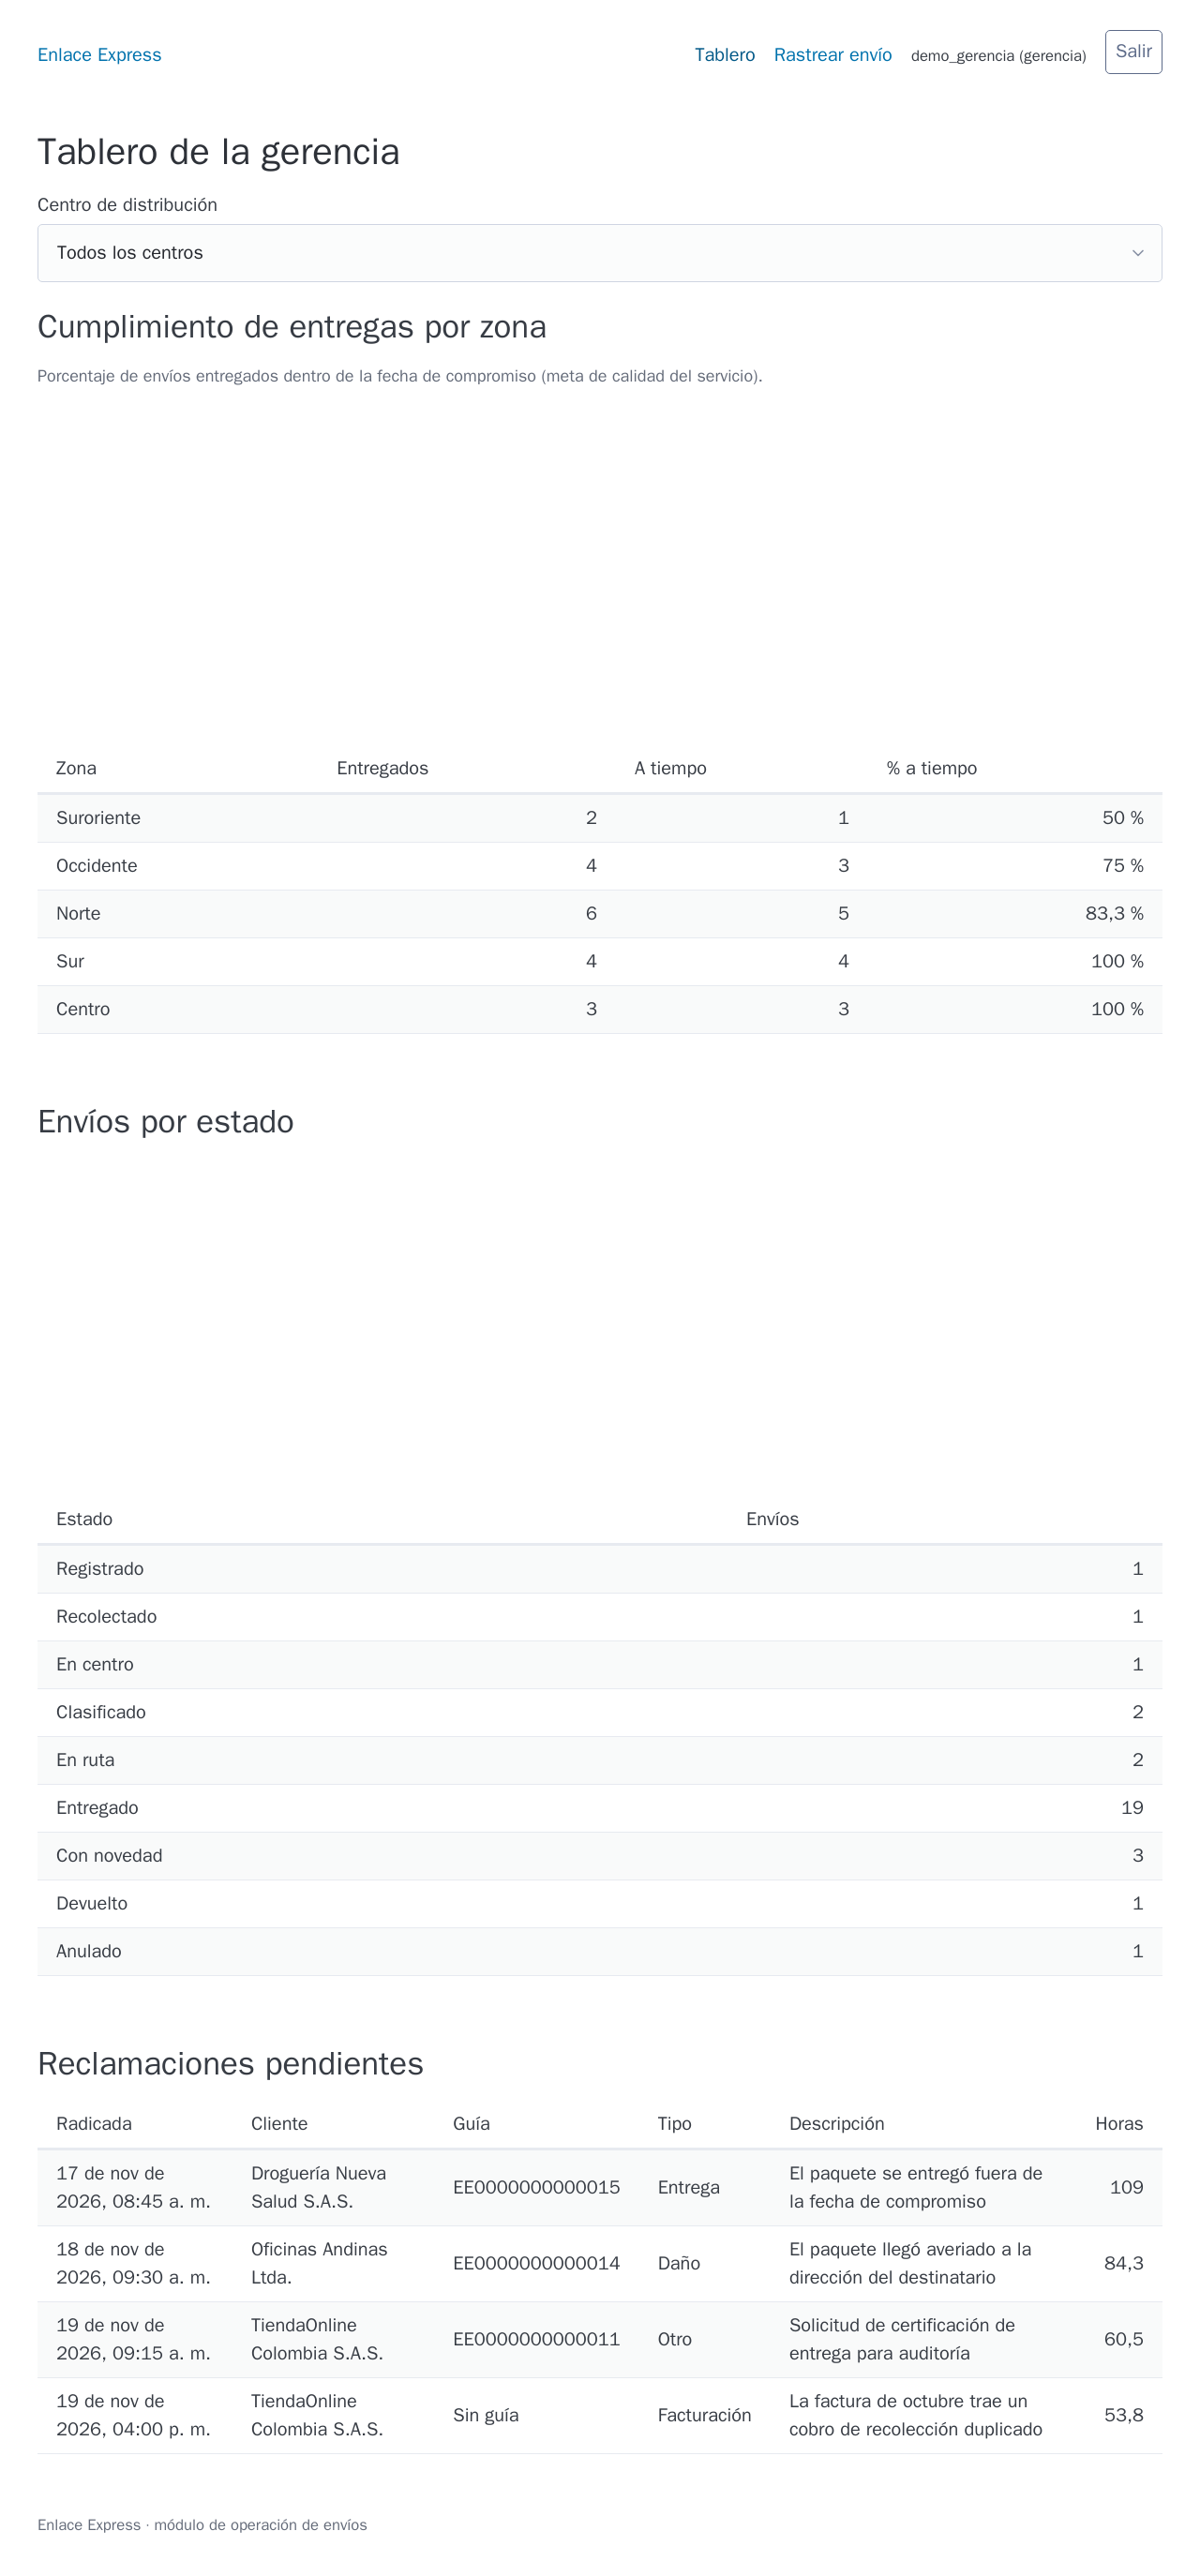
\includegraphics[trim=0 1138 0 0, clip, width=0.65\linewidth]{figuras/prototipo/16_tablero.png}
\caption{Tablero de la gerencia: cumplimiento de entregas por zona y envíos por estado.}
\label{fig:proto-tablero}
\end{figure}

La mesa de servicio también gestiona novedades y reclamaciones. En
\emph{Novedades} ve las novedades abiertas con los teléfonos del destinatario y
del cliente, decide si se reintenta o se devuelve, deja la solución y la
cierra. En \emph{Reclamaciones} radica la reclamación de un cliente, con
una guía opcional que debe ser de un envío de ese cliente (si no lo es, la
aplicación la rechaza), la responde y la cierra. La lista de pendientes marca
con las horas transcurridas las que superan la meta de cuatro horas de la
regla RN14 (figura~\ref{fig:proto-reclamaciones}). El personal del centro, por
su parte, administra los centros y sus zonas en \emph{Centros y zonas}: crea y
modifica, e inactiva un centro en lugar de borrarlo (RN16), y a un centro
inactivo no se le agregan zonas.

\begin{figure}[htbp]
\centering
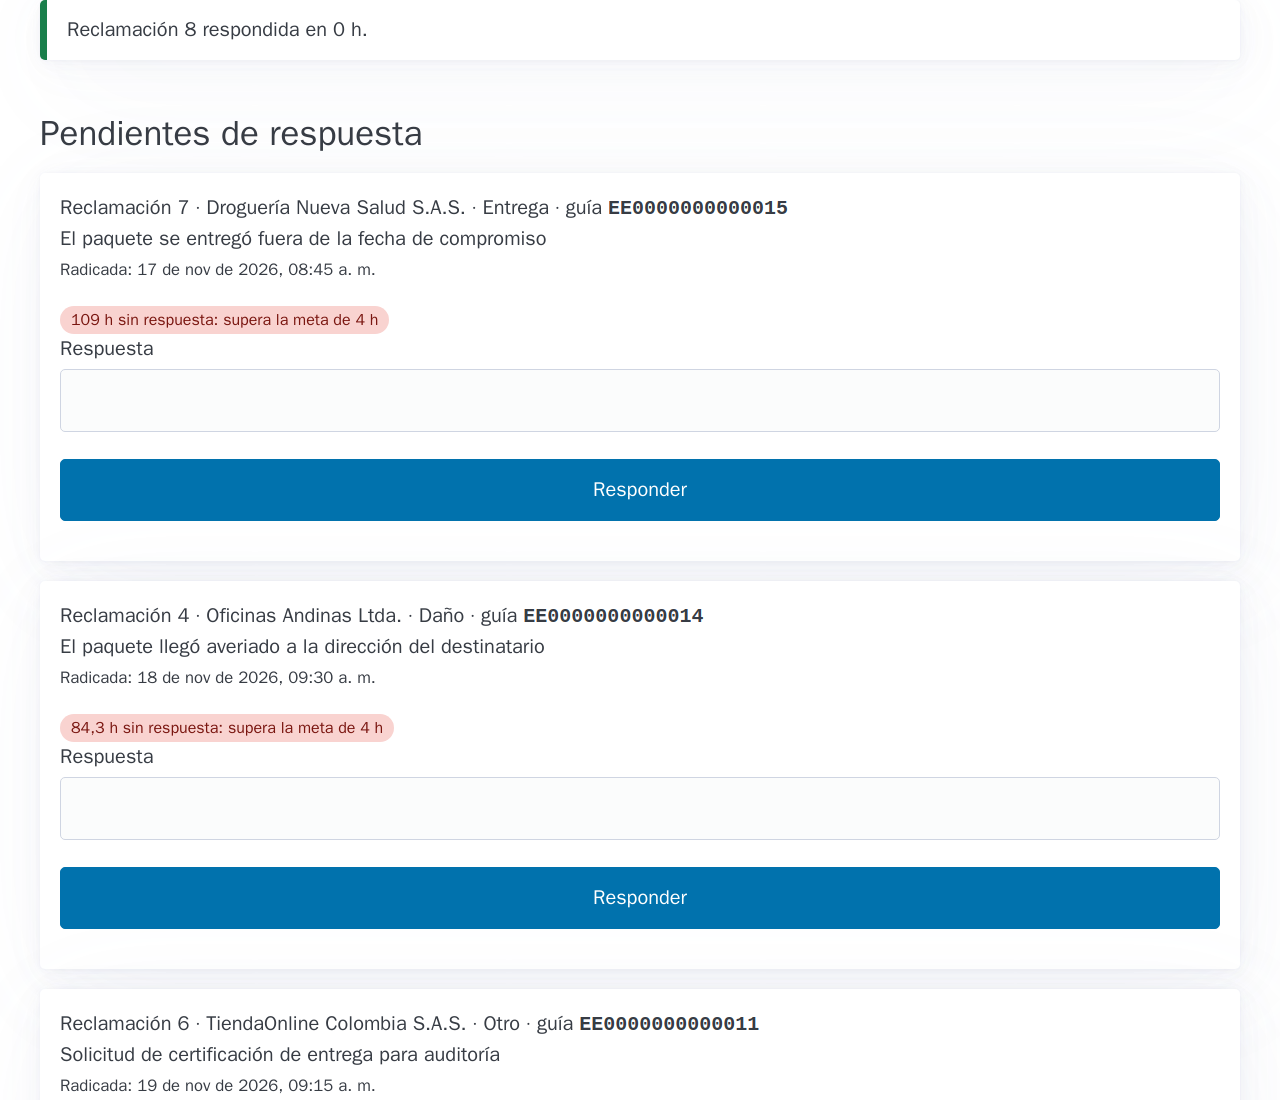
\includegraphics[width=0.7\linewidth]{figuras/prototipo/23_mesa_reclamacion_respondida.png}
\caption{Reclamaciones en la mesa de servicio: aviso de la respuesta registrada y pendientes con las horas transcurridas y la marca de la meta de 4 horas.}
\label{fig:proto-reclamaciones}
\end{figure}

El caso de rechazo sigue con el envío que tuvo novedad: el centro cierra el
despacho, el envío vuelve a la lista de envíos por despachar con un intento
previo y sale en un despacho nuevo; tras una segunda novedad y un tercer
despacho, en el intento 3 la planilla ya no ofrece entregar y solo permite
registrar la devolución (figura~\ref{fig:proto-tercer}), con la que el envío
queda devuelto. La mesa de servicio, por último, intenta anular un envío
ya entregado, y la transición bloqueada se ve en pantalla con el código RN12
(figura~\ref{fig:proto-rn12}).

\begin{figure}[htbp]
\centering
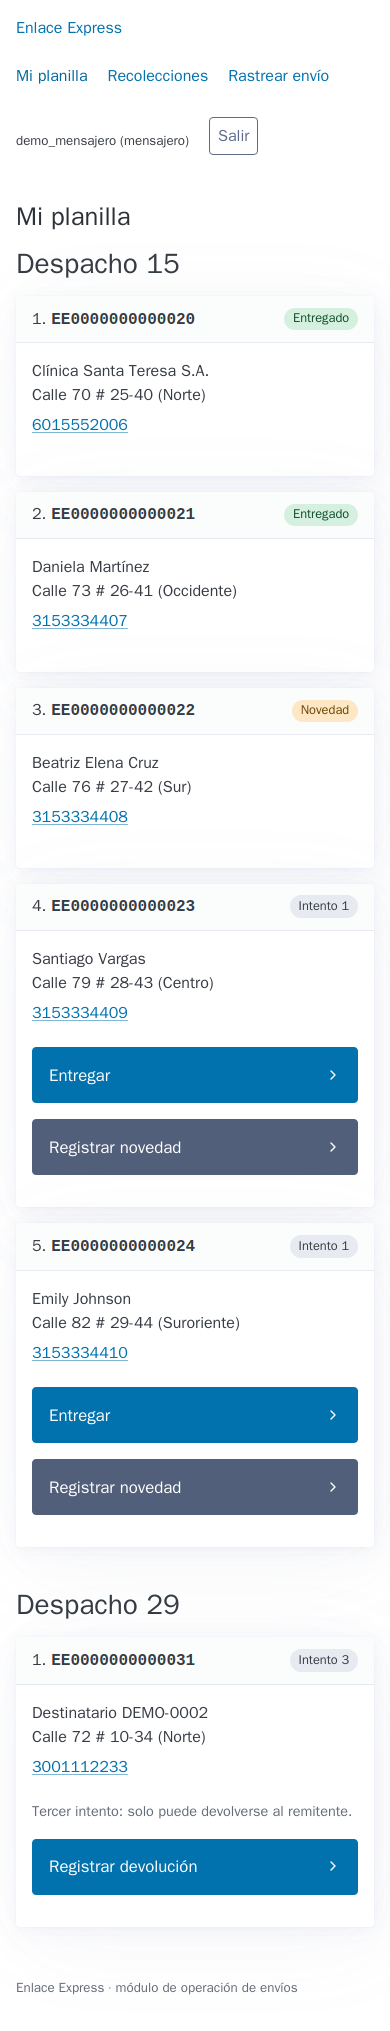
\includegraphics[trim=0 71 0 1560, clip, width=0.42\linewidth]{figuras/prototipo/18_mensajero_tercer_intento_movil.png}
\caption{Tercer intento en la planilla: solo se ofrece registrar la devolución.}
\label{fig:proto-tercer}
\end{figure}

\begin{figure}[htbp]
\centering
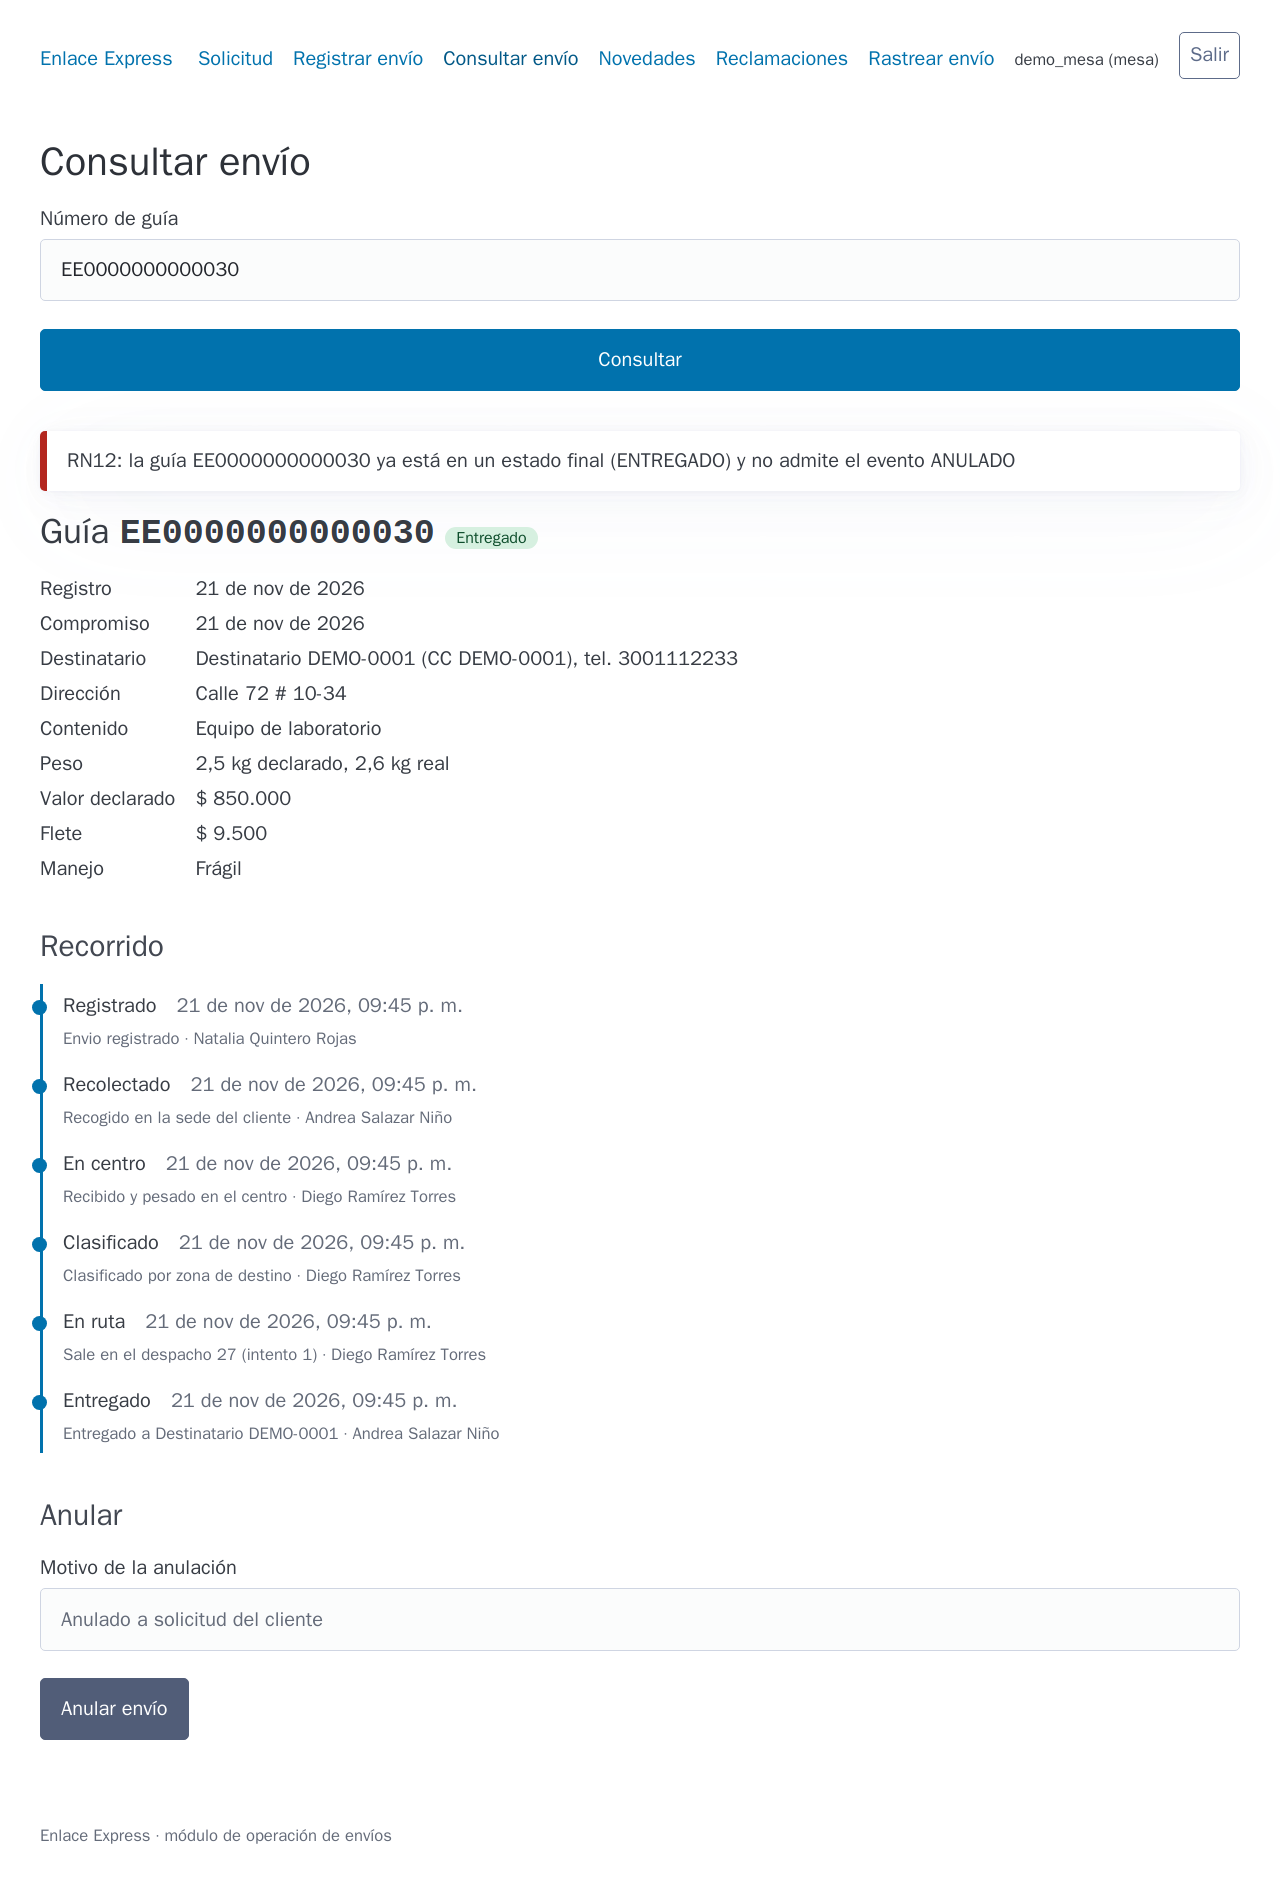
\includegraphics[trim=0 890 0 0, clip, width=0.75\linewidth]{figuras/prototipo/21_rechazo_rn12_anular_entregado.png}
\caption{Rechazo RN12 al intentar anular un envío ya entregado.}
\label{fig:proto-rn12}
\end{figure}

\textbf{Pruebas de la aplicación.} Hay tres niveles:

\begin{itemize}[itemsep=2pt]
  \item \textbf{Unitarias.} Las pruebas del dominio y de la infraestructura no
        usan la base de datos: 60 pruebas en 10 clases, que cubren las reglas
        del dominio (RN02, RN03, RN05, RN07, RN10, RN11, RN12, RN14 y RN15), el
        ciclo de vida del envío, la gestión de novedades y reclamaciones, los
        centros y las zonas, y la traducción de errores de Oracle.
  \item \textbf{De integración.} 39 pruebas en 8 clases que usan Oracle: los
        mapeadores y la unidad de trabajo contra la base (15) y la API por
        HTTP real con sesión y token CSRF (24), incluidos el flujo principal, los
        rechazos y la devolución en el tercer intento, los permisos por rol, el
        identificador de cliente, el rastreo público sin datos personales y el
        límite de consultas.
        Por defecto usan el Oracle del compose. Con la variable de entorno
        \texttt{ENLACE\_TESTCONTAINERS=true}, o con el perfil de Maven
        \texttt{testcontainers}, levantan en cambio un solo contenedor de
        Oracle, con la misma imagen, para toda la corrida: instalan el
        esquema con \texttt{database/install.sh}, generan sus contraseñas al azar y no
        dependen del compose ni del \texttt{.env}. Es el modo de la
        integración continua (subsección~\ref{sec:proto-despliegue}).
  \item \textbf{De punta a punta.} Un recorrido en un navegador sin
        cabeza (Chromium con Playwright) de 27 pasos con los usuarios de
        demostración, que da 27 OK y 0 fallas y guarda 25 capturas, de las
        que esta subsección usa once.
\end{itemize}

La tabla~\ref{tab:proto-pruebas} da el resultado de
\texttt{mvn verify} por clase: 99 pruebas, ninguna con falla. La
demostración se reconstruye con un solo comando,
\texttt{demo/start.sh}, que reinstala la base, compila la
aplicación, la levanta y crea un usuario de demostración por rol (gerencia,
centro, mesa, mensajero y cliente); la contraseña de esos usuarios sale de
una variable de entorno y no está en el repositorio ni en este documento.

% Fuente: docs/evidence/12_pruebas_backend.txt y docs/evidence/10_aplicacion/resumen.txt
{\singlespacing\small
\begin{longtable}{L{4.8cm} L{6.8cm} >{\raggedleft\arraybackslash}p{1.7cm}}
\caption{Pruebas automáticas de la aplicación, por clase.}
\label{tab:proto-pruebas}\\
\toprule
\textbf{Clase} & \textbf{Qué prueba} & \textbf{Pruebas} \\
\midrule
\endfirsthead
\toprule
\textbf{Clase} & \textbf{Qué prueba} & \textbf{Pruebas} \\
\midrule
\endhead
\bottomrule
\endfoot
ConversorTiposTest & Conversión de tipos entre Java y Oracle & 3 \\
TraductorErroresOracleTest & Conversión de errores de Oracle en excepciones del dominio & 11 \\
AsignacionDespachoTest & Intentos de entrega y sus resultados (RN05, RN07, RN08) & 8 \\
DespachoTest & Armado y cierre del despacho (RN10, RN11) & 6 \\
EnvioTest & Registro, clasificación, anulación y eventos del envío (RN02, RN03, RN05, RN12) & 8 \\
CicloDeVidaEnvioTest & Transiciones de estado (RN12) & 6 \\
SolicitudRecoleccionTest & Solicitud de recolección (RN15) & 4 \\
ReclamacionTest & Reclamaciones: radicar, responder (RN14), cerrar y la meta de 4 horas & 6 \\
NovedadTest & Gestión y cierre de la novedad & 3 \\
CentroZonaTest & Centros y zonas: validación, estado y zonas de centros inactivos & 5 \\
\midrule
\multicolumn{2}{l}{\textbf{Unitarias}} & \textbf{60} \\
\midrule
CatalogoEstadosIT & Los catálogos del dominio coinciden con los de la base & 2 \\
FlujoPrincipalIT & El flujo principal con los mapeadores contra Oracle & 2 \\
InfraestructuraJdbcIT & Cuentas de servicio, unidad de trabajo, identificador de cliente y traducción de errores & 11 \\
FlujoApiIT & Flujo principal por la API, rechazos y devolución en el tercer intento & 3 \\
GestionMesaCentroIT & Novedades, reclamaciones y centros y zonas por la API, con sus rechazos & 5 \\
OpenApiIT & La documentación OpenAPI y Swagger UI se entregan sin sesión y las rutas de los roles siguen protegidas & 3 \\
SaludIT & Chequeo de salud de la aplicación y la base & 1 \\
SeguridadIT & Registro, sesión, CSRF, roles, rastreo público y límite por dirección IP & 12 \\
\midrule
\multicolumn{2}{l}{\textbf{De integración}} & \textbf{39} \\
\midrule
\multicolumn{2}{l}{\textbf{Total}} & \textbf{99} \\
\end{longtable}
\par}


%-----------------------------------------------------------------------
\subsubsection{Extensiones fuera del módulo}
\label{sec:proto-extensiones}

El prototipo es el módulo de operación de envíos funcionando. Se permite
extenderlo fuera del módulo solo para probar un caso de uso completo o para
hacer una prueba real del sistema. Cada extensión se registra en
\texttt{docs/extensions.md} con lo que agrega, el caso de uso que permite
probar y por qué no está en el módulo; sus scripts van en una carpeta aparte,
\texttt{database/extensions}, y no modifican las 19 tablas del módulo. Se
hicieron dos extensiones, E1 y E2.

\textbf{E1. Usuarios de la aplicación y códigos de activación.} El módulo no
tiene credenciales: las cuentas de usuario y la autenticación no hacen
parte de la operación de envíos, y en una empresa real vendrían del
directorio de usuarios. Pero sin cuentas no se puede probar ningún caso
de uso que exija iniciar sesión (los de U1 a U4 y el seguimiento de U9 con
cuenta) ni la alta de cuentas del caso de uso de gestión de usuarios y
roles. Por eso se agregó E1, con los objetos de la
tabla~\ref{tab:proto-e1}.

{\singlespacing\small
\begin{longtable}{L{3.6cm} L{2.2cm} L{8.2cm}}
\caption{Objetos de la extensión E1.}
\label{tab:proto-e1}\\
\toprule
\textbf{Objeto} & \textbf{Tipo} & \textbf{Qué es} \\
\midrule
\endfirsthead
\toprule
\textbf{Objeto} & \textbf{Tipo} & \textbf{Qué es} \\
\midrule
\endhead
\bottomrule
\endfoot
USUARIO\_\allowbreak APLICACION & Tabla & Cuenta de acceso: nombre de usuario único, hash BCrypt de la contraseña, rol de la aplicación (GERENCIA, CENTRO, MESA, MENSAJERO o CLIENTE), vínculo con un empleado (una cuenta por empleado) o con un cliente (varias cuentas por empresa), estado y fechas de creación y de último ingreso. \\
CODIGO\_\allowbreak ACTIVACION & Tabla & Código de un solo uso y con vencimiento, emitido para un empleado o para un cliente. Solo se guarda su hash SHA-256; registra cuándo se usó y qué cuenta lo usó. \\
Cuatro índices & Índices & Sobre las claves foráneas, en TS\_ENLACE\_INDICES como los demás. \\
pkg\_codigos\_\allowbreak activacion & Paquete & Solo para el administrador de la base de datos: genera el código de un empleado activo (por documento) o de un cliente activo (por NIT), con vigencia de 72 horas por defecto. \\
pkg\_seguridad & Paquete & Lo usa la aplicación: registro de empleados y clientes con su código, datos para el inicio de sesión y registro del último ingreso. \\
\end{longtable}
\par}

Las dos tablas no se conceden a ningún rol: la única puerta es el paquete
\texttt{pkg\_seguridad}, con permiso de ejecución para el rol cliente. La
parte pública de la aplicación (inicio de sesión, registro y rastreo por
guía) trabaja antes de saber quién es el usuario, y usa la cuenta de
servicio de menor privilegio, \texttt{svc\_cliente}.

\textbf{Cómo se registra un usuario.} El administrador genera un código para
el empleado (con su documento) o para la empresa cliente (con su NIT) y se
lo entrega. La persona abre la aplicación y escribe su documento o el NIT
de su empresa, el código, un nombre de usuario y una contraseña. La
aplicación calcula el hash de la contraseña y llama a \texttt{pkg\_seguridad};
la base de datos nunca ve la contraseña, y del código solo guarda el hash, no el
código en claro, que se muestra una vez al generarlo. El código se usa una
sola vez.

\textbf{Reglas que aplica E1.}

\begin{itemize}[itemsep=2pt]
  \item El código es de un solo uso y vence. Se bloquea con
        \texttt{SELECT \ldots{} FOR UPDATE} al usarlo, para que dos
        registros simultáneos no lo usen dos veces.
  \item El empleado debe existir y estar ACTIVO, y el cliente debe estar
        ACTIVO.
  \item El rol se deriva del cargo y nunca lo elige el usuario: Gerente es
        GERENCIA, Auxiliar de centro es CENTRO, Agente de mesa de servicio
        es MESA y Mensajero, si tiene fila en MENSAJERO, es MENSAJERO. Otro
        cargo no tiene acceso.
  \item Un documento inexistente, un código ajeno, usado o vencido dan el
        mismo mensaje, para no revelar cuál dato falló.
  \item Una cuenta cuyo empleado se retira o cuyo cliente se inactiva queda
        INACTIVA de inmediato en el inicio de sesión.
  \item Los errores van en el rango ORA-20101 a ORA-20112, con mensajes que
        empiezan por \texttt{E1:}, fuera del rango de las reglas RN del
        módulo.
\end{itemize}

\textbf{Pruebas de E1.} El script
\texttt{database/tests/test-e1.sh} ejecuta 74 casos, todos con el
resultado previsto (tabla~\ref{tab:proto-pruebas-e1}). Incluyen, entre otros,
la reutilización de un código (ORA-20101), un código vencido o de otro
empleado, un empleado retirado, un nombre de usuario repetido (ORA-20102),
un cargo sin acceso (ORA-20103), una segunda cuenta para el mismo empleado
(ORA-20105) y que las otras cuatro cuentas de servicio no puedan leer ni
ejecutar nada de E1.

% Fuente: docs/evidence/09_extension_e1.txt
{\singlespacing\small
\begin{longtable}{L{9.0cm} >{\raggedleft\arraybackslash}p{1.6cm} >{\raggedleft\arraybackslash}p{1.8cm}}
\caption{Casos de prueba de la extensión E1.}
\label{tab:proto-pruebas-e1}\\
\toprule
\textbf{Parte} & \textbf{Casos} & \textbf{Fallas} \\
\midrule
\endfirsthead
\toprule
\textbf{Parte} & \textbf{Casos} & \textbf{Fallas} \\
\midrule
\endhead
\bottomrule
\endfoot
Lógica de los paquetes y restricciones de las tablas (propietario) & 48 & 0 \\
La aplicación con \texttt{svc\_cliente}: registro, inicio de sesión y permisos & 10 & 0 \\
Las otras cuatro cuentas de servicio no tienen acceso a E1 & 16 & 0 \\
\midrule
\textbf{Total} & \textbf{74} & \textbf{0} \\
\end{longtable}
\par}

{\sloppy
\textbf{E2. Vista de rastreo público.} El documento define el seguimiento
con la vista \texttt{v\_\allowbreak seguimiento\_\allowbreak envio}, para la mesa de servicio y
para el cliente con cuenta. Esa vista trae la observación y el responsable
de cada evento, que pueden contener nombres (por ejemplo, ``Entregado a
Recepción del edificio''), y no trae la zona. El rastreo público, que la
decisión de diseño pide sin cuenta y sin datos personales, necesita
la zona de destino, y la cuenta \texttt{svc\_\allowbreak cliente} no puede leer las tablas
ENVIO ni ZONA. En lugar de cambiar una de las siete vistas del módulo o
de ampliar los permisos del rol cliente, se agregó la vista
\texttt{v\_\allowbreak rastreo\_\allowbreak publico}: número de guía, identificador del evento
(solo para ordenar), fecha y hora, estado y zona de cada evento. Es de solo
lectura y se concede únicamente al rol cliente. No incluye la observación, el
responsable ni ningún dato del destinatario o del cliente.
\par}

Con E2 se prueba el seguimiento público de un envío sin cuenta: cualquier
persona con el número de guía ve estados, fechas y zona, sin nombres,
direcciones ni teléfonos. Como las guías son consecutivas y se podrían recorrer,
la aplicación limita además las consultas por dirección IP (30 por minuto por
defecto).

% Fuente: docs/evidence/03_prueba_permisos.txt (svc_cliente) y 01_verificacion_cifras.txt
Las pruebas de permisos de la subsección~\ref{sec:proto-bd} cubren E2: con
la cuenta \texttt{svc\_cliente}, la consulta de \texttt{v\_rastreo\_publico}
pasa, y leer las tablas ENVIO y ZONA se rechaza (ORA-00942). La
aplicación muestra el resultado en la captura del rastreo público de la
subsección~\ref{sec:proto-aplicacion}.

\textbf{Las cifras del módulo no cambian.} La verificación de cifras de
la tabla~\ref{tab:proto-cifras} cuenta los objetos del módulo por una lista
explícita, y con las extensiones instaladas sigue dando 19 tablas, 59
índices, 7 vistas, 6 disparadores y 1 procedimiento. Las extensiones
tienen sus propias filas, aparte: E1 agrega 2 tablas y ningún privilegio
concedido a los roles, y E2 agrega 1 vista; las tres dan OK
(tabla~\ref{tab:proto-cifras-ext}).

% Fuente: docs/evidence/01_verificacion_cifras.txt
{\singlespacing\small
\begin{longtable}{L{8.2cm} >{\raggedleft\arraybackslash}p{1.9cm} >{\raggedleft\arraybackslash}p{1.9cm} L{2.0cm}}
\caption{Cifras de las extensiones, aparte de las del módulo.}
\label{tab:proto-cifras-ext}\\
\toprule
\textbf{Cifra} & \textbf{Esperado} & \textbf{Obtenido} & \textbf{Resultado} \\
\midrule
\endfirsthead
\toprule
\textbf{Cifra} & \textbf{Esperado} & \textbf{Obtenido} & \textbf{Resultado} \\
\midrule
\endhead
\bottomrule
\endfoot
Extensión E1: tablas & 2 & 2 & OK \\
Extensión E1: privilegios concedidos a roles & 0 & 0 & OK \\
Extensión E2: vistas & 1 & 1 & OK \\
\end{longtable}
\par}


%-----------------------------------------------------------------------
\subsubsection{Concurrencia}
\label{sec:proto-concurrencia}

\textbf{El problema.} En la operación, dos usuarios pueden actuar al
mismo tiempo sobre el mismo envío o el mismo despacho. Por ejemplo, la mesa
de servicio anula un envío en el momento en que el centro lo incluye en un
despacho; o dos centros arman despachos que comparten un envío. Si cada
transacción lee el estado, decide y escribe sin coordinarse, las dos
pueden decidir con el mismo estado de partida y dejar el envío con eventos
que no siguen el ciclo de vida de la tabla~\ref{tab:transiciones}
(por ejemplo, EN\_RUTA después de ANULADO).

\textbf{La solución: bloqueo pesimista.} Toda transacción que cambia el
estado de un envío o de un despacho bloquea primero esa fila con
\texttt{SELECT \ldots{} FOR UPDATE}. Mientras una transacción tiene la
fila bloqueada, otra que quiera cambiarla espera; cuando la primera
confirma o deshace, la segunda sigue y, al leer, ve el estado que dejó la
primera. Así las reglas del dominio y los disparadores trabajan siempre
sobre el estado actual y la segunda transacción se rechaza, con el mensaje
de la regla correspondiente, si ya no es válida.

Se eligió el bloqueo pesimista en lugar del optimista por tres razones.
Las transacciones son cortas (cada operación toma una conexión al
empezar y la devuelve al terminar), de modo que el bloqueo dura milisegundos y nadie
espera mientras un usuario llena un formulario. Un conflicto sobre un mismo
envío es poco frecuente, pero sus consecuencias son costosas: eventos
fuera de orden o un envío entregado dos veces. Y el control optimista
exigiría una columna de versión en las tablas y repetir la operación
cuando alguien se anticipó, algo que el modelo no tiene y que complica la
aplicación sin beneficio para este volumen.

\textbf{Cómo lo aplican las transacciones y la aplicación.} Las
transacciones de la subsección~\ref{sec:proto-transacciones} empiezan con el
bloqueo de la fila que cambia. La aplicación hace lo mismo: cada caso de
uso abre una unidad de trabajo, que toma una conexión de la cuenta de
servicio del rol, sin confirmación automática; la transacción la maneja
la propia aplicación y no un marco externo. Cada operación bloquea,
antes de leer el estado y decidir, lo que muestra la
tabla~\ref{tab:proto-bloqueos}.

{\singlespacing\small
\begin{longtable}{L{5.0cm} L{9.0cm}}
\caption{Filas que bloquea cada operación de la aplicación.}
\label{tab:proto-bloqueos}\\
\toprule
\textbf{Operación} & \textbf{Filas bloqueadas, en orden} \\
\midrule
\endfirsthead
\toprule
\textbf{Operación} & \textbf{Filas bloqueadas, en orden} \\
\midrule
\endhead
\bottomrule
\endfoot
Registrar envío & La solicitud de recolección. \\
Anular un envío & El envío. \\
Recolectar & La solicitud y, uno por uno, sus envíos. \\
Recibir y clasificar & El envío. \\
Armar el despacho de entrega & Cada envío del despacho, en orden de número de guía. \\
Registrar entrega, novedad o devolución & El envío y la asignación. \\
Cerrar el despacho & El despacho. \\
\end{longtable}
\par}

\textbf{Orden de bloqueo.} Cuando una operación bloquea varias filas, dos
operaciones simultáneas podrían quedar esperándose una a la otra
(interbloqueo). Para evitarlo, al armar un despacho la aplicación elimina
las guías repetidas y las ordena por número de guía antes de bloquearlas, de
modo que dos despachos que compartan envíos los bloquean en el mismo
orden y uno simplemente espera al otro.

\textbf{Instantes distintos (C5).} El índice único sobre el número de guía
y la fecha y hora del evento impide que un envío tenga dos eventos en el
mismo instante. Cuando una transacción inserta varios eventos del mismo
envío, la aplicación asigna a cada uno un instante distinto, siempre
posterior al último evento de la guía; el tipo de dato guarda
microsegundos. Las transacciones de prueba hacen lo mismo con una función
que calcula ese instante:

\begin{lstlisting}[style=sqlpro]
FUNCTION instante(p_guia IN VARCHAR2) RETURN TIMESTAMP IS
    v_i TIMESTAMP;
BEGIN
    SELECT GREATEST(LOCALTIMESTAMP,
                    NVL(MAX(fecha_hora), LOCALTIMESTAMP) + INTERVAL '1' SECOND)
    INTO   v_i FROM evento_envio WHERE numero_guia = p_guia;
    RETURN v_i;
END instante;
\end{lstlisting}

\textbf{La prueba.} El script \texttt{database/transactions/concurrency.sh}
reproduce el conflicto con dos sesiones de verdad sobre el envío
EE0000000000028. La sesión A, con la cuenta del centro
(\texttt{svc\_centro}), bloquea la fila con \texttt{SELECT \ldots{} FOR UPDATE}
y no confirma. La sesión B, con la cuenta de la mesa (\texttt{svc\_mesa}),
intenta lo mismo con la opción \texttt{NOWAIT}, que en lugar de esperar
devuelve el error ORA-00054 (recurso ocupado), y reintenta cada segundo.
Se usa \texttt{NOWAIT} solo para que el conflicto quede a la vista sin dejar
una sesión colgada; la aplicación, en cambio, espera el bloqueo. Si Oracle
devuelve ORA-00054 a la aplicación, esta lo traduce a una respuesta de
conflicto. La tabla~\ref{tab:proto-concurrencia} muestra la línea de
tiempo: B recibe ORA-00054 en los seis intentos que hace mientras A tiene
la fila; cuando A deshace, B consigue el bloqueo en el intento 7.

% Fuente: docs/evidence/06_transacciones/concurrencia.txt
{\singlespacing\small
\begin{longtable}{L{2.4cm} L{1.4cm} L{9.6cm}}
\caption{Línea de tiempo de la prueba de concurrencia.}
\label{tab:proto-concurrencia}\\
\toprule
\textbf{Hora} & \textbf{Sesión} & \textbf{Hecho} \\
\midrule
\endfirsthead
\toprule
\textbf{Hora} & \textbf{Sesión} & \textbf{Hecho} \\
\midrule
\endhead
\bottomrule
\endfoot
16:59:34.534 & A & Obtiene el bloqueo sobre EE0000000000028, sin COMMIT. \\
16:59:35.037 & B & Intento 1 rechazado: ORA-00054, la fila está bloqueada por A. \\
16:59:36.038 & B & Intento 2 rechazado: ORA-00054. \\
16:59:37.038 & B & Intento 3 rechazado: ORA-00054. \\
16:59:38.039 & B & Intento 4 rechazado: ORA-00054. \\
16:59:39.039 & B & Intento 5 rechazado: ORA-00054. \\
16:59:40.040 & B & Intento 6 rechazado: ORA-00054. \\
16:59:40.537 & A & ROLLBACK, bloqueo liberado. \\
16:59:41.040 & B & Intento 7 consigue el bloqueo sobre EE0000000000028. \\
16:59:41.041 & B & ROLLBACK (la prueba no modifica datos). \\
\end{longtable}
\par}

\textbf{Las restricciones siguen siendo la garantía final.} El bloqueo
evita que dos transacciones decidan con el mismo estado, pero no es la
única defensa. Si dos transacciones llegaran a escribir a la vez lo mismo,
la base de datos las rechaza por sus restricciones: una segunda prueba de
entrega o una segunda novedad para el mismo intento viola una restricción
UNIQUE (ORA-00001, casos de T6 y T7), y dos eventos de una guía en el mismo
instante violan el índice único de guía y fecha y hora. Los disparadores
validan el ciclo de vida en la base aunque la aplicación se saltara el
dominio. Por eso las reglas de negocio no dependen de que todas las
aplicaciones bloqueen bien.


%-----------------------------------------------------------------------
\subsubsection{Despliegue y CI/CD}
\label{sec:proto-despliegue}
% Actualizar cuando se cree la máquina virtual y el dominio o se active el CD (los artefactos ya existen y se probaron en el equipo)

\textbf{Estado actual.} Hoy el prototipo corre en el equipo de desarrollo:
Oracle Database 23c Free en un contenedor Docker, definido en el archivo
\texttt{docker-compose.yml}, y la aplicación como un programa Java. Los
artefactos para publicarlo en un servidor existen y se probaron en el equipo
(más abajo), pero todavía no hay una máquina virtual ni un dominio. Todo se
reconstruye desde cero con tres comandos:

\begin{enumerate}[itemsep=2pt]
  \item \texttt{docker compose up -d} levanta la base de datos y espera a que
        esté lista.
  \item \texttt{database/install.sh} reinstala el esquema, los datos y las
        extensiones, y verifica las cifras del documento. Como alternativa,
        \texttt{demo/start.sh} hace además la aplicación: la
        compila, la levanta y crea los usuarios de demostración.
  \item \texttt{database/generate-evidence.sh} repite las pruebas, las consultas, las
        transacciones y los informes y regenera todas las evidencias de
        \texttt{docs/evidence/}.
\end{enumerate}

Las contraseñas no están en el repositorio: salen de un archivo \texttt{.env}
que no se versiona, del que solo se guarda una plantilla. El
contenedor usa la zona horaria America/Bogota, igual que la aplicación.

\textbf{Integración continua.} {\sloppy El flujo de GitHub Actions es el archivo
\texttt{ci.yml} de la carpeta \texttt{.github/workflows}. Se ejecuta en cada cambio a la rama
principal y en cada solicitud de integración, en una máquina Ubuntu del
servicio, y tiene dos trabajos que corren en paralelo:\par}

\begin{itemize}[itemsep=2pt]
  \item \textbf{Compilar y probar.} Prepara Java 21 y Node 22, compila el
        frontend, y compila el backend y corre sus 99 pruebas con
        \texttt{mvn verify}. Las pruebas de integración usan Testcontainers:
        levantan un solo contenedor de Oracle con la misma imagen que usa el
        compose, instalan el esquema con \texttt{database/install.sh}, que verifica
        las cifras del documento en modo estricto, y apuntan la aplicación y las
        pruebas a ese contenedor. Si algo falla, guarda los informes de las
        pruebas.
  \item \textbf{Cifras del documento.} Instala el esquema en un Oracle
        desechable y falla si alguna de las cifras del documento (19 tablas, 59
        índices, 6 disparadores, etc.) no coincide.
\end{itemize}

El flujo no usa secretos: las contraseñas de Oracle se generan al azar en cada
corrida y viajan por variables de entorno. Las mismas pruebas pueden correrse
en el equipo, contra el Oracle del compose (modo normal) o con
Testcontainers, que no depende de él. Como el repositorio no tiene un
servidor remoto, el flujo no se ha ejecutado en GitHub: se validó su sintaxis
y se ejecutaron sus mismos pasos en el equipo con \texttt{ci/local.sh}, que
compila el frontend, corre \texttt{mvn verify} con Testcontainers y verifica las
cifras, de principio a fin, sin fallas y en unos dos minutos
(\texttt{docs/evidence/12\_pruebas\_backend.txt}).

\textbf{Artefactos de despliegue.} La carpeta \texttt{deploy/} reúne lo
necesario para publicar el prototipo según el diseño definido, y se probó en el
equipo:

\begin{itemize}[itemsep=2pt]
  \item \textbf{Imagen de la aplicación.} El \texttt{Dockerfile} es multietapa:
        compila el frontend (Node 22) y el backend (Maven con JDK 21) y deja un
        JRE 21 con versión fija, un usuario sin privilegios, la zona horaria
        America/Bogota y una comprobación de salud contra \texttt{/api/salud}.
        Las imágenes base son para x86 y ARM. Aquí se construyó para x86; la de
        ARM no se construyó porque el equipo no tiene el emulador QEMU, y la
        construirá el flujo de entrega continua.
  \item \textbf{Compose de producción.} Levanta Oracle 23c Free con un volumen
        con nombre y sin publicar su puerto, la aplicación y Caddy (con versión
        fija) como proxy inverso. Las contraseñas y el dominio salen de un
        archivo \texttt{.env}.
  \item \textbf{HTTPS.} Caddy obtiene y renueva el certificado del dominio
        configurado; con el dominio \texttt{localhost} usa su certificado
        interno, lo que permitió probarlo en el equipo. La aplicación va detrás
        del proxy con las cookies marcadas como seguras y con el límite de
        consultas del rastreo público calculado por la dirección IP que agrega
        el proxy.
  \item \textbf{Esquema.} Un script instala el esquema una sola vez y no hace
        nada si ya existe; un cambio de esquema se hace reinstalando con él.
  \item \textbf{Entrega continua.} El flujo de GitHub Actions \texttt{cd.yml}
        se ejecuta cuando la integración continua de la rama principal termina
        bien: construye la imagen para x86 y ARM, la publica en el registro de
        contenedores de GitHub y, si hay un servidor configurado con sus
        secretos, actualiza por SSH solo los contenedores de la aplicación. Como
        el repositorio no tiene un servidor remoto, el flujo no se ha ejecutado;
        solo se validó su sintaxis.
  \item \textbf{Respaldo.} Si no se consigue la máquina virtual, se presenta
        desde el equipo propio con Docker y un túnel de Cloudflare, que da
        HTTPS gratuito pero no tiene entrega continua; el procedimiento está
        explicado en \texttt{deploy/README.md}.
\end{itemize}

\textbf{Prueba en el equipo.} El script \texttt{deploy/test-local.sh}
construye la imagen, levanta el compose de producción con el dominio
\texttt{localhost}, instala el esquema, hace las comprobaciones de la
tabla~\ref{tab:proto-despliegue} con \texttt{curl} a través de Caddy y, al terminar,
baja el compose y borra sus volúmenes. Dio 21 de 21 comprobaciones correctas.
Entre ellas, que el límite de consultas cuenta la dirección IP real de cada
cliente y no la del proxy: desde el equipo, las primeras 30 consultas dan 200 y la
31 da 429, un encabezado \texttt{X-Forwarded-For} falso no evita el límite, y
otro cliente con otra dirección, desde otro contenedor, sigue consultando.

% Fuente: docs/evidence/14_despliegue_local.txt
{\singlespacing\small
\begin{longtable}{L{4.0cm} L{9.2cm}}
\caption{Comprobaciones de la prueba local del despliegue.}
\label{tab:proto-despliegue}\\
\toprule
\textbf{Aspecto} & \textbf{Comprobación (todas dieron OK)} \\
\midrule
\endfirsthead
\toprule
\textbf{Aspecto} & \textbf{Comprobación (todas dieron OK)} \\
\midrule
\endhead
\bottomrule
\endfoot
Imagen & Se construye; la aplicación corre sin privilegios, con la zona horaria America/Bogota. \\
Oracle & Está sano y no publica ningún puerto; la aplicación solo se alcanza por Caddy. \\
Esquema & Se instala con las cifras del documento en modo estricto y una segunda ejecución no lo reinstala. \\
HTTPS & \texttt{/api/salud} responde 200 por HTTPS, HTTP redirige a HTTPS, Caddy agrega Strict-Transport-Security y se sirve la aplicación web. \\
Rastreo público & La guía EE0000000000003 muestra su estado ENTREGADO sin sesión. \\
Rutas protegidas & \texttt{/api/mesa/clientes} da 401 sin sesión y 200 con la sesión de la mesa, creada con un código de activación. \\
Cookies & Las cookies \texttt{XSRF-TOKEN} y \texttt{JSESSIONID} salen con Secure, y la de sesión con HttpOnly. \\
Límite por IP & 30 consultas dan 200 y la 31 da 429; un \texttt{X-Forwarded-For} falso no evita el límite; otro cliente con otra IP no queda limitado. \\
\end{longtable}
\par}

\textbf{Lo que falta.} Quedan por hacer, y requieren las cuentas del autor,
crear la máquina virtual gratuita de Oracle Cloud (Ampere A1), el subdominio
de DuckDNS y los secretos del repositorio que usa la entrega continua. Los pasos
están en \texttt{deploy/README.md}.

Se descartaron otras opciones: Vercel, porque no aloja Oracle y su modelo de
funciones no encaja con una sesión guardada en el servidor; Render con el plan
gratuito, porque tiene 512 MB de memoria, se apaga tras 15 minutos sin
tráfico y no tiene Oracle; y Autonomous Database gratuita, porque no permite
crear espacios de tablas, lo que contradice el diseño físico del
capítulo~5.



\newpage

%------------------------------- ANEXOS --------------------------------
\appendix
\counterwithin{figure}{section}
\counterwithin{table}{section}
\titleformat{\section}{\normalfont\normalsize\bfseries}{ANEXO \thesection.}{1em}{\MakeUppercase}
\addtocontents{toc}{\protect\vspace{0.6em}\noindent\textbf{ANEXOS}\par}

%======================================================================
%  Anexo A - Analisis de los modulos no priorizados
%======================================================================

\section{Análisis de los módulos no priorizados}
\label{anx:analisis}

Este anexo conserva el análisis de requerimientos de los módulos M2
(comercial y facturación), M3 (flota) y M4 (talento humano), que se
implementarán después del módulo de operación.

\subsection{Actividades de los procesos P4 a P8}

{\singlespacing\small
\begin{longtable}{L{1.3cm} L{6.3cm} L{2.9cm} L{3.9cm}}
\caption{Actividades de los procesos P4 a P8.}
\label{tab:actividadesotros}\\
\toprule
\textbf{Código} & \textbf{Actividad} & \textbf{Responsable} & \textbf{Información que usa o genera} \\
\midrule
\endfirsthead
\toprule
\textbf{Código} & \textbf{Actividad} & \textbf{Responsable} & \textbf{Información que usa o genera} \\
\midrule
\endhead
\bottomrule
\endfoot
\multicolumn{4}{l}{\textit{SP4.1 Vinculación de clientes y sedes}} \\*
A4.1.1 & Registrar los datos del cliente: NIT, razón social, tipo de cliente y contacto. & Asesor comercial & Cliente \\
A4.1.2 & Registrar las sedes de recolección del cliente con su zona. & Asesor comercial & Sede del cliente, zona \\
A4.1.3 & Actualizar o inactivar clientes. & Asesor comercial & Cliente \\
\midrule
\multicolumn{4}{l}{\textit{SP4.2 Contratos y tarifas}} \\*
A4.2.1 & Definir las modalidades del servicio y su plazo de entrega. & Jefe comercial & Modalidad \\
A4.2.2 & Registrar el contrato con sus fechas de vigencia y plazo de pago. & Asesor comercial & Contrato, cliente \\
A4.2.3 & Pactar las tarifas por zona, rango de peso y modalidad. & Asesor comercial & Tarifa, zona, modalidad \\
A4.2.4 & Renovar o terminar contratos. & Asesor comercial & Contrato \\
\midrule
\multicolumn{4}{l}{\textit{SP5.1 Facturación mensual}} \\*
A5.1.1 & Seleccionar los envíos entregados o devueltos del mes que aún no han sido facturados. & Auxiliar de facturación & Envío, cliente \\
A5.1.2 & Generar la factura con el valor de cada envío, el subtotal, el IVA y el total. & Auxiliar de facturación & Factura, envío, contrato \\
A5.1.3 & Anular una factura con errores y registrar el motivo. & Auxiliar de facturación & Factura \\
\midrule
\multicolumn{4}{l}{\textit{SP5.2 Recaudo y cartera}} \\*
A5.2.1 & Registrar los pagos recibidos y actualizar el estado de la factura. & Auxiliar de cartera & Pago, factura \\
A5.2.2 & Consultar la cartera por cliente, separando las facturas con reclamación abierta. & Auxiliar de cartera & Factura, pago, cliente, reclamación \\
\midrule
\multicolumn{4}{l}{\textit{SP6.1 Registro de vehículos}} \\*
A6.1.1 & Registrar el vehículo: tipo, placa, marca, capacidad, si es eléctrico y centro asignado. & Coordinador de flota & Vehículo, centro de distribución \\
\midrule
\multicolumn{4}{l}{\textit{SP6.2 Control documental}} \\*
A6.2.1 & Registrar los documentos de cada vehículo con su fecha de vencimiento. & Auxiliar de control documental & Documento del vehículo, vehículo \\
A6.2.2 & Consultar los documentos próximos a vencer. & Auxiliar de control documental & Documento del vehículo \\
\midrule
\multicolumn{4}{l}{\textit{SP6.3 Mantenimiento}} \\*
A6.3.1 & Programar los mantenimientos preventivos. & Coordinador de flota & Mantenimiento, vehículo \\
A6.3.2 & Registrar el mantenimiento realizado y cambiar el estado del vehículo. & Técnico de taller & Mantenimiento, vehículo \\
\midrule
\multicolumn{4}{l}{\textit{SP7.1 Vinculación y retiro de personal}} \\*
A7.1.1 & Registrar al empleado con su cargo, centro, zona (si es mensajero) y fecha de ingreso. & Analista de talento humano & Empleado, centro de distribución, zona \\
A7.1.2 & Registrar el retiro del empleado con fecha y motivo. & Analista de talento humano & Empleado \\
\midrule
\multicolumn{4}{l}{\textit{SP7.2 Control de licencias y capacitaciones}} \\*
A7.2.1 & Registrar la licencia de conducción de los mensajeros: número, categoría y vencimiento. & Analista de talento humano & Empleado \\
A7.2.2 & Programar capacitaciones y registrar la asistencia y el resultado de cada empleado. & Analista de SST & Capacitación, empleado \\
\midrule
\multicolumn{4}{l}{\textit{SP8.1 Cálculo y seguimiento de indicadores}} \\*
A8.1.1 & Calcular el porcentaje de entregas a tiempo y de envíos con novedad por centro, zona y periodo. & Gerente general & Envío, evento de seguimiento, novedad, modalidad \\
A8.1.2 & Calcular el tiempo de respuesta a reclamaciones y el porcentaje de facturas con reclamo. & Gerente general & Reclamación, factura, cliente \\
A8.1.3 & Calcular la rotación de mensajeros y la participación de vehículos eléctricos. & Gerente general & Empleado, vehículo, centro de distribución \\
\end{longtable}
\par}

\subsection{Entradas, procesos y salidas de sus usuarios}

{\singlespacing\small
\begin{longtable}{L{1.9cm} L{3.9cm} L{4.6cm} L{3.9cm}}
\caption{Entradas, procesos y salidas de los usuarios de los módulos no priorizados.}
\label{tab:epsotros}\\
\toprule
\textbf{Usuario} & \textbf{Entradas} & \textbf{Procesos} & \textbf{Salidas} \\
\midrule
\endfirsthead
\toprule
\textbf{Usuario} & \textbf{Entradas} & \textbf{Procesos} & \textbf{Salidas} \\
\midrule
\endhead
\bottomrule
\endfoot
U5 Flota y mantenimiento &
Datos de vehículos; documentos con fechas de vencimiento; mantenimientos
programados y realizados. &
Cambiar el estado del vehículo al entrar y salir de mantenimiento;
detectar documentos que vencen en los próximos 15 días. &
Vehículos disponibles por centro; alertas de vencimiento; historial y
costo de mantenimiento por vehículo. \\
\midrule
U6 Asesor comercial &
Datos de clientes y sedes; contratos; modalidades; tarifas por zona,
modalidad y rango de peso. &
Validar que no haya rangos de peso superpuestos en un mismo contrato,
zona y modalidad; controlar la vigencia de los contratos. &
Tarifario por cliente; contratos próximos a vencer; volumen de envíos
por cliente y zona. \\
\midrule
U7 Facturación y cartera &
Periodo a facturar; pagos recibidos; anulaciones de factura. &
Agrupar los envíos entregados o devueltos no facturados; calcular
subtotal, IVA y total; impedir que un envío se facture dos veces;
actualizar el saldo de la factura con cada pago. &
Facturas del periodo; estado de cartera por edades; facturas con
reclamación abierta. \\
\midrule
U8 Talento humano &
Datos de empleados; retiros; licencias; capacitaciones y asistencia. &
Calcular la vigencia de la capacitación anual; detectar licencias
vencidas o próximas a vencer. &
Mensajeros habilitados para salir a ruta; rotación de personal;
cumplimiento del plan de capacitación. \\
\end{longtable}
\par}

\subsection{Permisos de todos los usuarios}

{\singlespacing
\begin{table}[H]
\centering
\footnotesize
\setlength{\tabcolsep}{1.3pt}
\renewcommand{\arraystretch}{1.25}
\begin{tabular}{l l c c c c c c c c c c c c c c c c c c c c c}
\toprule
\multicolumn{2}{l}{\textbf{Usuario}} & \rotatebox{90}{\textbf{E01}} & \rotatebox{90}{\textbf{E02}} & \rotatebox{90}{\textbf{E03}} & \rotatebox{90}{\textbf{E04}} & \rotatebox{90}{\textbf{E05}} & \rotatebox{90}{\textbf{E06}} & \rotatebox{90}{\textbf{E07}} & \rotatebox{90}{\textbf{E08}} & \rotatebox{90}{\textbf{E09}} & \rotatebox{90}{\textbf{E10}} & \rotatebox{90}{\textbf{E11}} & \rotatebox{90}{\textbf{E12}} & \rotatebox{90}{\textbf{E13}} & \rotatebox{90}{\textbf{E14}} & \rotatebox{90}{\textbf{E15}} & \rotatebox{90}{\textbf{E16}} & \rotatebox{90}{\textbf{E17}} & \rotatebox{90}{\textbf{E18}} & \rotatebox{90}{\textbf{E19}} & \rotatebox{90}{\textbf{E20}} & \rotatebox{90}{\textbf{E21}} \\
\midrule
U1 & Gerente general & L & L & L &  & L & L &  &  & L & L & L &  & L & L & L & L & L &  &  & L &  \\
U2 & Personal de centro & CA & CA &  & L & L & L & L & A & A & C & CA &  &  &  &  &  & L & L &  & A & L \\
U3 & Mesa de servicio &  & L & L & L & L & L &  & C & CA & CL &  &  & A & CA & L &  &  &  &  &  &  \\
U4 & Mensajero &  &  &  & L &  &  &  & A & A & C & L & C & C &  &  &  &  &  &  &  &  \\
U5 & Flota y mantenimiento & L &  &  &  &  &  &  &  &  &  & L &  &  &  &  &  & CA & CA & CA &  &  \\
U6 & Asesor comercial &  & L & CA & CA & CA & CA & CA &  &  &  &  &  &  &  &  &  &  &  &  &  &  \\
U7 & Facturación y cartera &  &  & L &  & L &  &  &  & A &  &  &  &  & L & CA & C &  &  &  &  &  \\
U8 & Talento humano & L & L &  &  &  &  &  &  &  &  &  &  &  &  &  &  &  &  &  & CA & CA \\
U9 & Cliente (externo) &  &  &  &  &  &  &  &  & L & L &  &  &  &  &  &  &  &  &  &  &  \\
\bottomrule
\end{tabular}
\caption{Operaciones de todos los usuarios sobre las 21 entidades del prediseño global (C: crear, L: leer, A: actualizar).}
\label{tab:permisosglobal}
\end{table}
\par}


\newpage

%======================================================================
%  Anexo B - Modelo conceptual global
%======================================================================

\section{Modelo conceptual global}
\label{anx:global}

Este anexo conserva el diseño conceptual de toda la empresa, del que se
extrajo el módulo priorizado. Las figuras siguen la notación descrita
al inicio del capítulo 3.

\subsection{Vistas por usuario}

La vista U4 está completa dentro del módulo (figura~\ref{fig:vistaU4}
y, en notación de Chen, figura~\ref{fig:vistaU4chen});
las vistas U2 y U3 se muestran aquí completas, con las entidades de
otros módulos (documentos del vehículo y capacitaciones en U2; contrato
y factura en U3).

\textbf{U5 -- Flota y mantenimiento:} el vehículo, dónde está asignado,
sus documentos, sus mantenimientos y los despachos en que se usó.
\textbf{U6 -- Asesor comercial:} el cliente, sus sedes, el contrato y
las tarifas por zona y modalidad. \textbf{U7 -- Facturación y cartera:}
ve los envíos como envíos \textit{del cliente} (relación
\textit{envía}), junto con pagos y reclamaciones. \textbf{U8 -- Talento
humano:} el empleado, su centro y sus capacitaciones con el resultado;
la zona y la licencia aparecen como atributos del empleado.

{\singlespacing
\begin{figure}[!htb]
\centering
\adjustbox{max width=\linewidth, max totalheight=0.42\textheight}{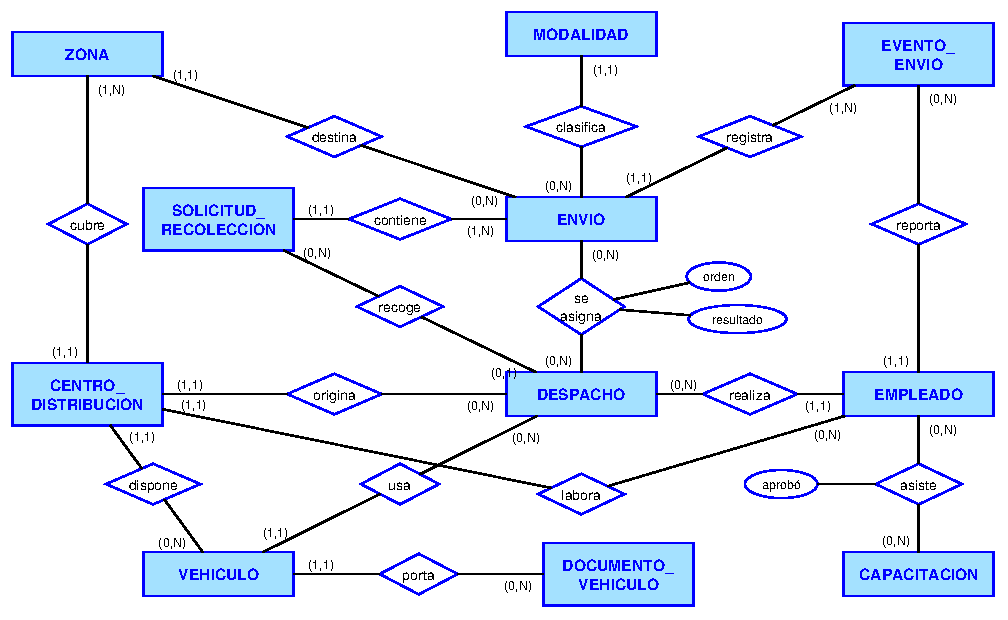
\includegraphics{figuras/er/U2.pdf}}
\caption{Vista U2 completa: personal del centro de distribución.}
\label{fig:vistaU2global}
\end{figure}
\par}
{\singlespacing
\begin{figure}[!htb]
\centering
\adjustbox{max width=\linewidth, max totalheight=0.42\textheight}{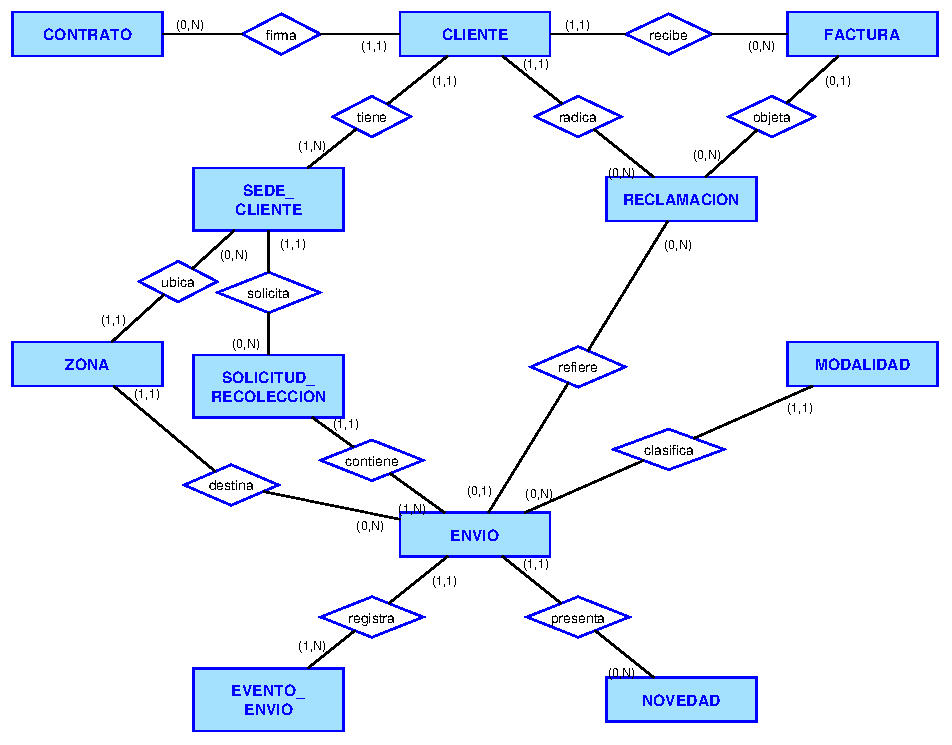
\includegraphics{figuras/er/U3.pdf}}
\caption{Vista U3 completa: mesa de servicio.}
\label{fig:vistaU3global}
\end{figure}
\par}
{\singlespacing
\begin{figure}[!htb]
\centering
\adjustbox{max width=\linewidth, max totalheight=0.3\textheight}{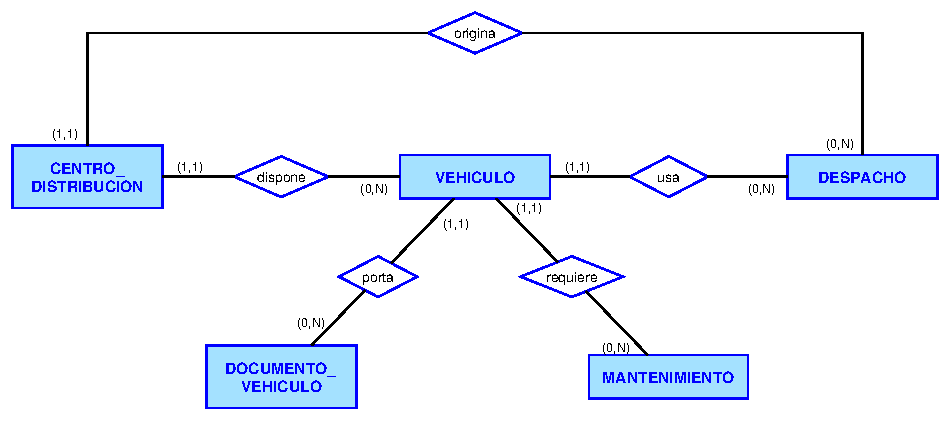
\includegraphics{figuras/er/U5.pdf}}
\caption{Vista U5: flota y mantenimiento.}
\label{fig:vistaU5}
\end{figure}
\par}
{\singlespacing
\begin{figure}[!htb]
\centering
\adjustbox{max width=\linewidth, max totalheight=0.3\textheight}{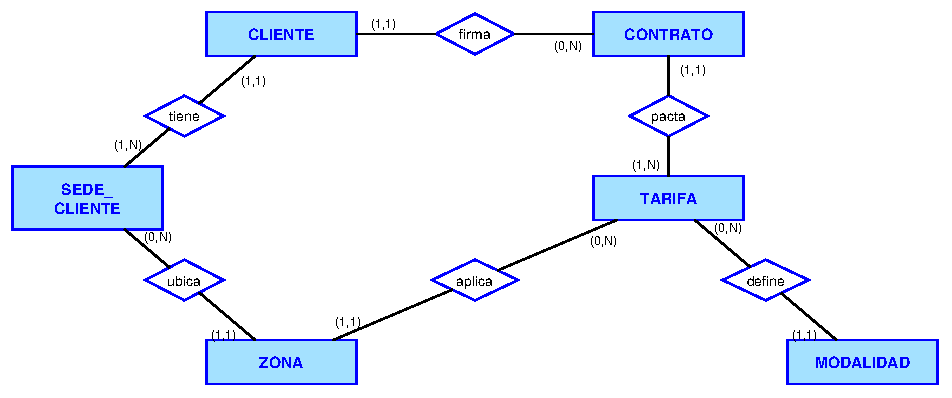
\includegraphics{figuras/er/U6.pdf}}
\caption{Vista U6: asesor comercial.}
\label{fig:vistaU6}
\end{figure}
\par}
{\singlespacing
\begin{figure}[!htb]
\centering
\adjustbox{max width=\linewidth, max totalheight=0.36\textheight}{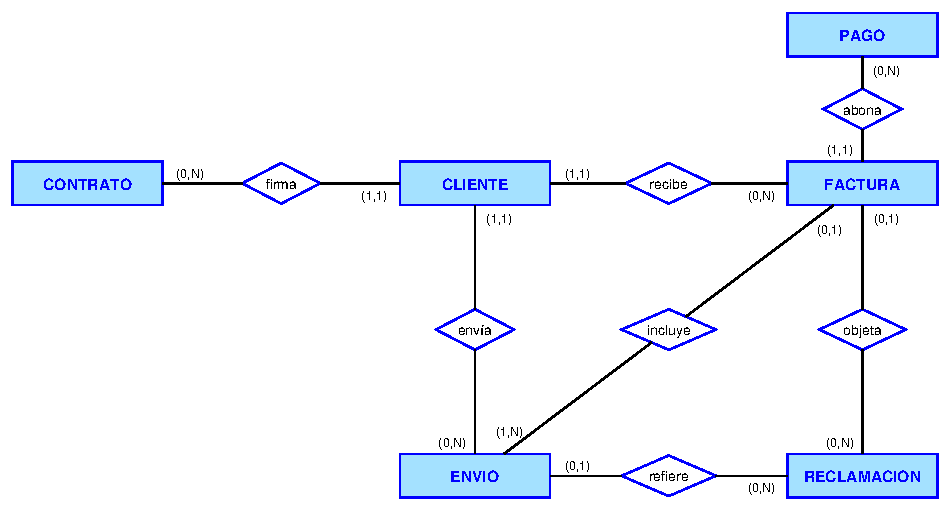
\includegraphics{figuras/er/U7.pdf}}
\caption{Vista U7: facturación y cartera.}
\label{fig:vistaU7}
\end{figure}
\par}
{\singlespacing
\begin{figure}[!htb]
\centering
\adjustbox{max width=\linewidth, max totalheight=0.2\textheight}{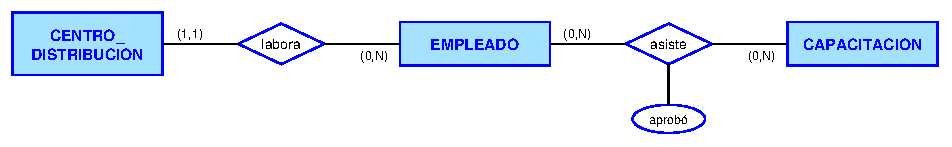
\includegraphics{figuras/er/U8.pdf}}
\caption{Vista U8: talento humano.}
\label{fig:vistaU8}
\end{figure}
\par}

\subsection{Prediseño global}

Integra las siete vistas con diagrama (U2 a U8): 21 entidades y 31
relaciones (figura~\ref{fig:erintegradoglobal} y
tabla~\ref{tab:relacionesglobal}). La relación directa
CLIENTE--\textit{envía}--ENVIO de la vista U7 se eliminó porque se
obtiene recorriendo CLIENTE--\allowbreak SEDE\_CLIENTE--\allowbreak SOLICITUD\_RECOLECCION--\allowbreak ENVIO;
guardar ambas permitiría asociar un envío a un cliente distinto del que
lo solicitó. Todas las demás vistas son subconjuntos del prediseño. La
zona fija del mensajero queda como atributo de EMPLEADO (defecto que
corrige el ajuste 3).

{\singlespacing\small
\begin{longtable}{L{1.5cm} L{5.0cm} L{2.2cm} L{5.4cm}}
\caption{Relaciones del prediseño global.}
\label{tab:relacionesglobal}\\
\toprule
\textbf{Relación} & \textbf{Entidades} & \textbf{(mín,máx)} & \textbf{Significado} \\
\midrule
\endfirsthead
\toprule
\textbf{Relación} & \textbf{Entidades} & \textbf{(mín,máx)} & \textbf{Significado} \\
\midrule
\endhead
\bottomrule
\endfoot
\textit{cubre} & CENTRO\_DISTRIBUCION --\allowbreak\ ZONA & (1,1) -- (1,N) & Cada zona es atendida por un solo centro. \\
\textit{labora} & CENTRO\_DISTRIBUCION --\allowbreak\ EMPLEADO & (1,1) -- (0,N) & Cada empleado trabaja en un centro. \\
\textit{dispone} & CENTRO\_DISTRIBUCION --\allowbreak\ VEHICULO & (1,1) -- (0,N) & Cada vehículo está asignado a un centro. \\
\textit{origina} & CENTRO\_DISTRIBUCION --\allowbreak\ DESPACHO & (1,1) -- (0,N) & Cada despacho sale de un centro. \\
\textit{ubica} & ZONA --\allowbreak\ SEDE\_CLIENTE & (1,1) -- (0,N) & Cada sede del cliente está en una zona. \\
\textit{destina} & ZONA --\allowbreak\ ENVIO & (1,1) -- (0,N) & Zona a la que va cada envío. \\
\textit{aplica} & ZONA --\allowbreak\ TARIFA & (1,1) -- (0,N) & Zona a la que corresponde cada tarifa. \\
\textit{tiene} & CLIENTE --\allowbreak\ SEDE\_CLIENTE & (1,1) -- (1,N) & Sedes de recolección de cada cliente. \\
\textit{firma} & CLIENTE --\allowbreak\ CONTRATO & (1,1) -- (0,N) & Contratos que ha tenido cada cliente. \\
\textit{pacta} & CONTRATO --\allowbreak\ TARIFA & (1,1) -- (1,N) & Tarifas acordadas en cada contrato. \\
\textit{define} & MODALIDAD --\allowbreak\ TARIFA & (1,1) -- (0,N) & Modalidad a la que corresponde cada tarifa. \\
\textit{clasifica} & MODALIDAD --\allowbreak\ ENVIO & (1,1) -- (0,N) & Modalidad contratada para cada envío. \\
\textit{solicita} & SEDE\_CLIENTE --\allowbreak\ SOLICITUD\_RECOLECCION & (1,1) -- (0,N) & Solicitudes hechas desde cada sede. \\
\textit{contiene} & SOLICITUD\_RECOLECCION --\allowbreak\ ENVIO & (1,1) -- (1,N) & Envíos que se recogen en cada solicitud. \\
\textit{recoge} & DESPACHO --\allowbreak\ SOLICITUD\_RECOLECCION & (0,1) -- (0,N) & Despacho de recolección que atiende cada solicitud. \\
\textit{se asigna} & ENVIO --\allowbreak\ DESPACHO & (0,N) -- (0,N) & Un envío puede salir en varios despachos (reintentos) y un despacho lleva muchos envíos. Atributos: orden, resultado. \\
\textit{registra} & ENVIO --\allowbreak\ EVENTO\_ENVIO & (1,1) -- (1,N) & Historial de estados de cada envío. \\
\textit{reporta} & EMPLEADO --\allowbreak\ EVENTO\_ENVIO & (1,1) -- (0,N) & Empleado responsable de cada evento. \\
\textit{soporta} & ENVIO --\allowbreak\ PRUEBA\_ENTREGA & (1,1) -- (0,1) & Constancia de recibo de cada envío. \\
\textit{presenta} & ENVIO --\allowbreak\ NOVEDAD & (1,1) -- (0,N) & Novedades ocurridas con cada envío. \\
\textit{radica} & CLIENTE --\allowbreak\ RECLAMACION & (1,1) -- (0,N) & Reclamaciones hechas por cada cliente. \\
\textit{refiere} & ENVIO --\allowbreak\ RECLAMACION & (0,1) -- (0,N) & Envío sobre el que trata una reclamación (opcional). \\
\textit{objeta} & FACTURA --\allowbreak\ RECLAMACION & (0,1) -- (0,N) & Factura sobre la que trata una reclamación (opcional). \\
\textit{recibe} & CLIENTE --\allowbreak\ FACTURA & (1,1) -- (0,N) & Facturas emitidas a cada cliente. \\
\textit{incluye} & FACTURA --\allowbreak\ ENVIO & (0,1) -- (1,N) & Factura en la que se cobra cada envío. \\
\textit{abona} & FACTURA --\allowbreak\ PAGO & (1,1) -- (0,N) & Pagos aplicados a cada factura. \\
\textit{porta} & VEHICULO --\allowbreak\ DOCUMENTO\_VEHICULO & (1,1) -- (0,N) & Documentos de cada vehículo. \\
\textit{requiere} & VEHICULO --\allowbreak\ MANTENIMIENTO & (1,1) -- (0,N) & Mantenimientos de cada vehículo. \\
\textit{usa} & VEHICULO --\allowbreak\ DESPACHO & (1,1) -- (0,N) & Vehículo con el que se hace cada despacho. \\
\textit{realiza} & EMPLEADO --\allowbreak\ DESPACHO & (1,1) -- (0,N) & Empleado (mensajero) que hace cada despacho. \\
\textit{asiste} & EMPLEADO --\allowbreak\ CAPACITACION & (0,N) -- (0,N) & Capacitaciones de cada empleado. Atributo: aprobó. \\
\end{longtable}
\par}

\begin{landscape}
{\singlespacing
\begin{figure}[p]
\centering
\adjustbox{max width=22.5cm, max totalheight=14.6cm}{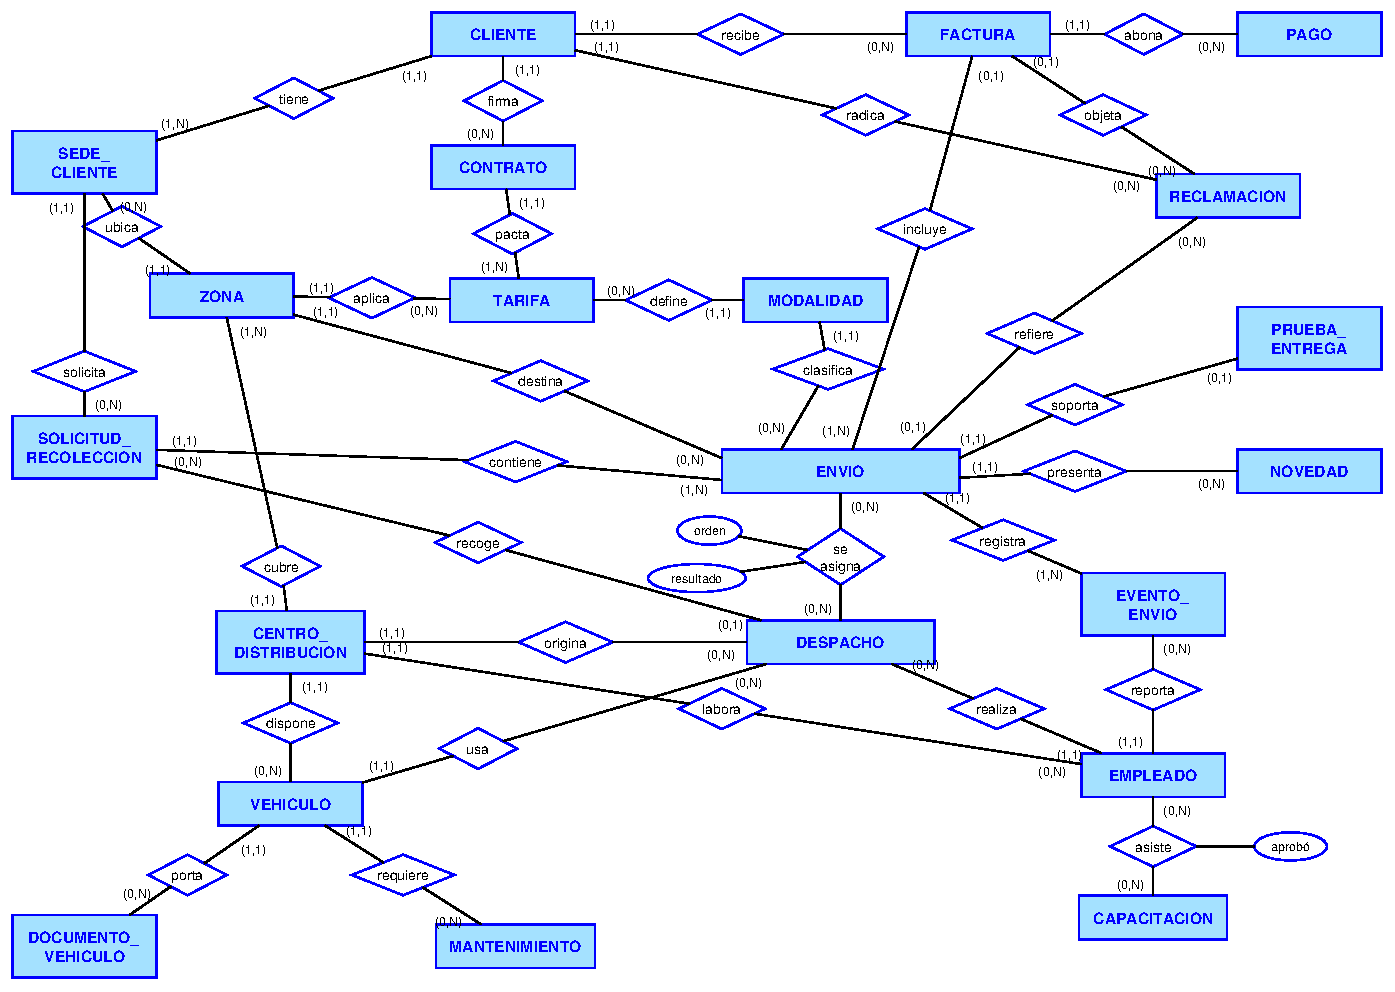
\includegraphics{figuras/er/prediseno.pdf}}
\caption{Prediseño conceptual global de BD\_ENLACE\_EXPRESS.}
\label{fig:erintegradoglobal}
\end{figure}
\par}
\end{landscape}


\subsection{Modelo ajustado global}

Con los ajustes 1 a 5 de la tabla~\ref{tab:ajustes}, el modelo global
pasa de 21 a 28 entidades. Se presenta en dos figuras según los grupos
de afinidad: la parte comercial y de operación (grupos G2, G3 y G4) y la
de recursos (G1, G5 y G6). Las entidades con fondo gris y borde punteado
aparecen en las dos figuras y se detallan en la otra. La
tabla~\ref{tab:atributosajustados} lista las entidades nuevas o
modificadas.

\begin{landscape}
{\singlespacing
\begin{figure}[p]
\centering
\adjustbox{max width=22.5cm, max totalheight=14.6cm}{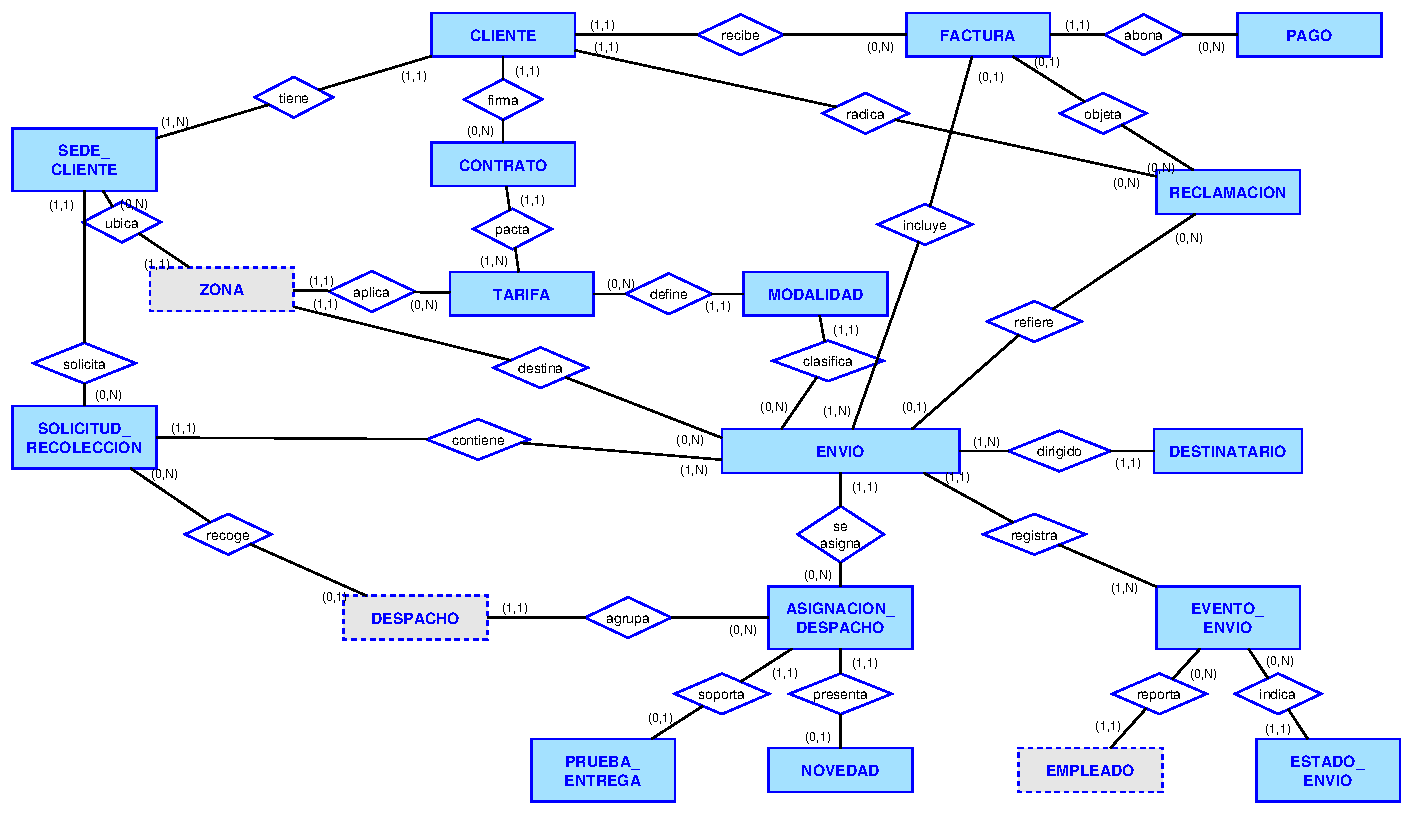
\includegraphics{figuras/er/ajustadoA.pdf}}
\caption{Modelo ajustado global: parte comercial y de operación de envíos.}
\label{fig:erfinalA}
\end{figure}
\par}
\end{landscape}
\begin{landscape}
{\singlespacing
\begin{figure}[p]
\centering
\adjustbox{max width=22.5cm, max totalheight=14.6cm}{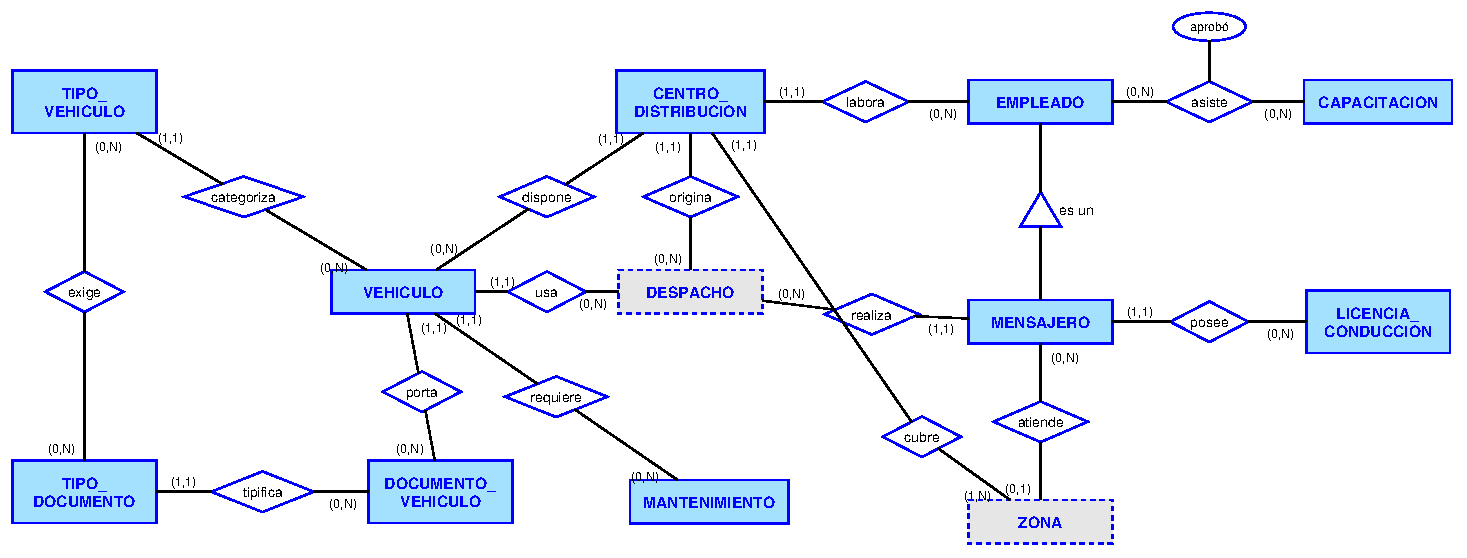
\includegraphics{figuras/er/ajustadoB.pdf}}
\caption{Modelo ajustado global: parte de recursos (centros, flota y personal).}
\label{fig:erfinalB}
\end{figure}
\par}
\end{landscape}
{\singlespacing\small
\begin{longtable}{L{3.6cm} L{3.4cm} L{7.4cm}}
\caption{Entidades nuevas o modificadas por los ajustes.}
\label{tab:atributosajustados}\\
\toprule
\textbf{Entidad} & \textbf{Estado} & \textbf{Atributos} \\
\midrule
\endfirsthead
\toprule
\textbf{Entidad} & \textbf{Estado} & \textbf{Atributos} \\
\midrule
\endhead
\bottomrule
\endfoot
DESTINATARIO & Nueva (ajuste 1) & id\_destinatario, tipo y número de documento, nombre, teléfono, correo \\
ENVIO & Modificada (ajustes 1 y 4) & número de guía, fecha de registro, dirección de destino, peso declarado, peso real, contenido, valor declarado, frágil, alto valor, valor del flete, fecha de compromiso \\
ASIGNACION\_\allowbreak DESPACHO & Nueva (ajuste 2) & id\_asignación, número de intento, orden de visita, hora de visita, resultado (pendiente, entregado, novedad, devuelto) \\
PRUEBA\_\allowbreak ENTREGA & Modificada (ajuste 2) & id\_prueba, fecha y hora, nombre y documento de quien recibe, tipo de prueba, archivo de soporte \\
NOVEDAD & Modificada (ajuste 2) & id\_novedad, tipo de novedad, descripción, acción (reintento o devolución), solución, estado \\
EMPLEADO & Modificada (ajuste 3) & id\_empleado, documento, nombres, apellidos, cargo, teléfono, correo, fecha de ingreso, fecha de retiro, motivo de retiro, estado \\
MENSAJERO & Nueva (ajuste 3) & id\_empleado (el mismo del empleado), tipo de vehículo que puede conducir \\
LICENCIA\_\allowbreak CONDUCCION & Nueva (ajuste 3) & id\_licencia, número, categoría, fecha de expedición, fecha de vencimiento \\
ESTADO\_ENVIO & Nueva (ajuste 4) & id\_estado, nombre (Registrado, Recolectado, En centro, Clasificado, En ruta, Entregado, Con novedad, Devuelto, Anulado), es final \\
EVENTO\_ENVIO & Modificada (ajuste 4) & id\_evento, fecha y hora, observación \\
TIPO\_VEHICULO & Nueva (ajuste 5) & id\_tipo\_vehículo, nombre (motocicleta, furgoneta, bicicleta eléctrica), capacidad máxima en kg \\
TIPO\_\allowbreak DOCUMENTO & Nueva (ajuste 5) & id\_tipo\_documento, nombre (SOAT, revisión técnico-mecánica, póliza, tarjeta de propiedad) \\
VEHICULO & Modificada (ajuste 5) & id\_vehículo, placa, marca, modelo, capacidad en kg, eléctrico, estado \\
DOCUMENTO\_\allowbreak VEHICULO & Modificada (ajuste 5) & id\_documento, número, fecha de expedición, fecha de vencimiento \\
\end{longtable}
\par}



\newpage

%======================================================================
%  Anexo C - Implementacion del modelo global en la herramienta CASE
%======================================================================

\section{Implementación del modelo global en la herramienta CASE}
\label{anx:case}


El modelo se implementó en Oracle SQL Developer Data Modeler, la
herramienta CASE del curso. En ella se equivalen los nombres de la
siguiente manera: lo que la herramienta llama \textit{Logical Model}
corresponde al modelo conceptual de este capítulo (entidades, atributos
y relaciones), y lo que llama \textit{Relational Model} corresponde al
modelo lógico del capítulo 4 (tablas, claves primarias y claves
foráneas).

En la herramienta se construyeron tres diseños: el prediseño
(figura~\ref{fig:erintegradoglobal}), la vista U7
(figura~\ref{fig:vistaU7}) y el modelo ajustado
(figuras~\ref{fig:erfinalA} y~\ref{fig:erfinalB}). Como las vistas U2,
U3, U4, U5, U6 y U8 son subconjuntos del prediseño
(sección~\ref{sec:integracion}), se construyeron como subvistas
(\textit{SubViews}) del diseño del prediseño; la vista U7 tiene su propio
diseño porque incluye la relación CLIENTE--\textit{envía}--ENVIO, que no
pasó al modelo integrado.

La herramienta representa el modelo en notación Barker. La
tabla~\ref{tab:barker} muestra su equivalencia con la notación de Chen
usada en el capítulo 3.

{\singlespacing
\begin{longtable}{L{4.0cm} L{5.4cm} L{5.0cm}}
\caption{Equivalencia entre la notación Barker de Data Modeler y la notación de Chen.}
\label{tab:barker}\\
\toprule
\textbf{Elemento} & \textbf{Barker (Data Modeler)} & \textbf{Chen (capítulo 3)} \\
\midrule
\endfirsthead
\toprule
\textbf{Elemento} & \textbf{Barker (Data Modeler)} & \textbf{Chen (capítulo 3)} \\
\midrule
\endhead
\bottomrule
\endfoot
Entidad & Rectángulo de esquinas redondeadas con el nombre y la lista de atributos & Rectángulo con el nombre \\
Atributo obligatorio u opcional & Marcado con \texttt{*} (obligatorio) u \texttt{o} (opcional) & No se dibuja; está en las tablas~\ref{tab:entidades} y~\ref{tab:atributosajustados} \\
Identificador & \texttt{P} (identificador principal) y \texttt{U} (valor único) & Primer atributo de la tabla de entidades \\
Relación & Línea entre las dos entidades, sin nombre visible & Rombo con el nombre de la relación \\
Cardinalidad máxima N & Pata de gallo en el extremo de la entidad & N en la pareja (mín, máx) \\
Participación & Mitad de línea continua: obligatoria; discontinua: opcional & Mínimo 1 u 0 en la pareja (mín, máx) \\
Relación identificadora & Barra transversal en el extremo de la entidad dependiente & No aplica en este modelo \\
Relación N:M con atributos & Entidad intermedia con dos relaciones identificadoras & Rombo con elipses de atributos \\
\end{longtable}
\par}

Al comparar los diagramas de la herramienta con los de Chen se deben
tener en cuenta cuatro diferencias, que se deben a la notación y no a
cambios en el modelo:

\begin{enumerate}[label=\arabic*.,leftmargin=1.2cm]
  \item \textbf{Relaciones N:M.} Las relaciones \textit{se asigna},
        \textit{asiste} y \textit{exige} aparecen como las entidades
        intermedias ENVIO\_DESPACHO, ASISTENCIA y DOCUMENTO\_EXIGIDO. Por
        eso el prediseño tiene 23 entidades en la herramienta (21 en
        Chen) y el modelo ajustado tiene 30 (28 en Chen).
  \item \textbf{Mínimo del lado ``uno''.} Una clave foránea no puede
        exigir que un registro padre tenga al menos un hijo, así que la
        herramienta dibuja siempre como opcional el extremo del lado
        ``uno''. Las
        relaciones \textit{tiene}, \textit{pacta}, \textit{contiene},
        \textit{registra}, \textit{incluye}, \textit{cubre} y
        \textit{dirigido} tienen mínimo 1 en ese lado en el modelo de
        Chen; esa regla se controlará en el diseño físico.
  \item \textbf{Especialización.} MENSAJERO aparece como una relación 1:1
        identificadora con EMPLEADO, porque su identificador es el mismo
        del empleado. Representa la misma especialización parcial de la
        figura~\ref{fig:erfinalB}.
  \item \textbf{Claves foráneas.} El modelo lógico de la herramienta no
        muestra las columnas de clave foránea; estas aparecen en el modelo
        relacional del capítulo 4.
\end{enumerate}

Cada diagrama de la herramienta se verificó contra su diagrama de Chen,
relación por relación. Los resultados de la tabla~\ref{tab:verificacion}
coinciden en todos los casos en entidades, relaciones, cardinalidad
máxima y participación del lado ``muchos''.

{\singlespacing
\begin{table}[H]
\centering
\caption{Verificación de los diagramas de Data Modeler.}
\label{tab:verificacion}
\small
\begin{tabular}{L{5.6cm} L{2.8cm} c c c}
\toprule
\textbf{Diagrama} & \textbf{Diseño} & \textbf{Entidades} & \textbf{Relaciones} & \textbf{Figura} \\
\midrule
Vista U2 -- Personal del centro & Prediseño & 13 & 17 & \ref{fig:dmU2} \\
Vista U3 -- Mesa de servicio & Prediseño & 11 & 14 & \ref{fig:dmU3} \\
Vista U4 -- Mensajero & Prediseño & 10 & 11 & \ref{fig:vistaU4} (cap. 3) \\
Vista U5 -- Flota & Prediseño & 5 & 5 & \ref{fig:dmU5} \\
Vista U6 -- Comercial & Prediseño & 6 & 6 & \ref{fig:dmU6} \\
Vista U7 -- Facturación y cartera & Vista U7 & 6 & 7 & \ref{fig:dmU7} \\
Vista U8 -- Talento humano & Prediseño & 4 & 3 & \ref{fig:dmU8} \\
Modelo ajustado & Ajustado & 30 & 42 & \ref{fig:dmajustado} \\
\bottomrule
\end{tabular}
\end{table}
\par}

\begin{landscape}
{\singlespacing
\begin{figure}[p]
\centering
\adjustbox{max width=22.5cm, max totalheight=14.6cm}{%%
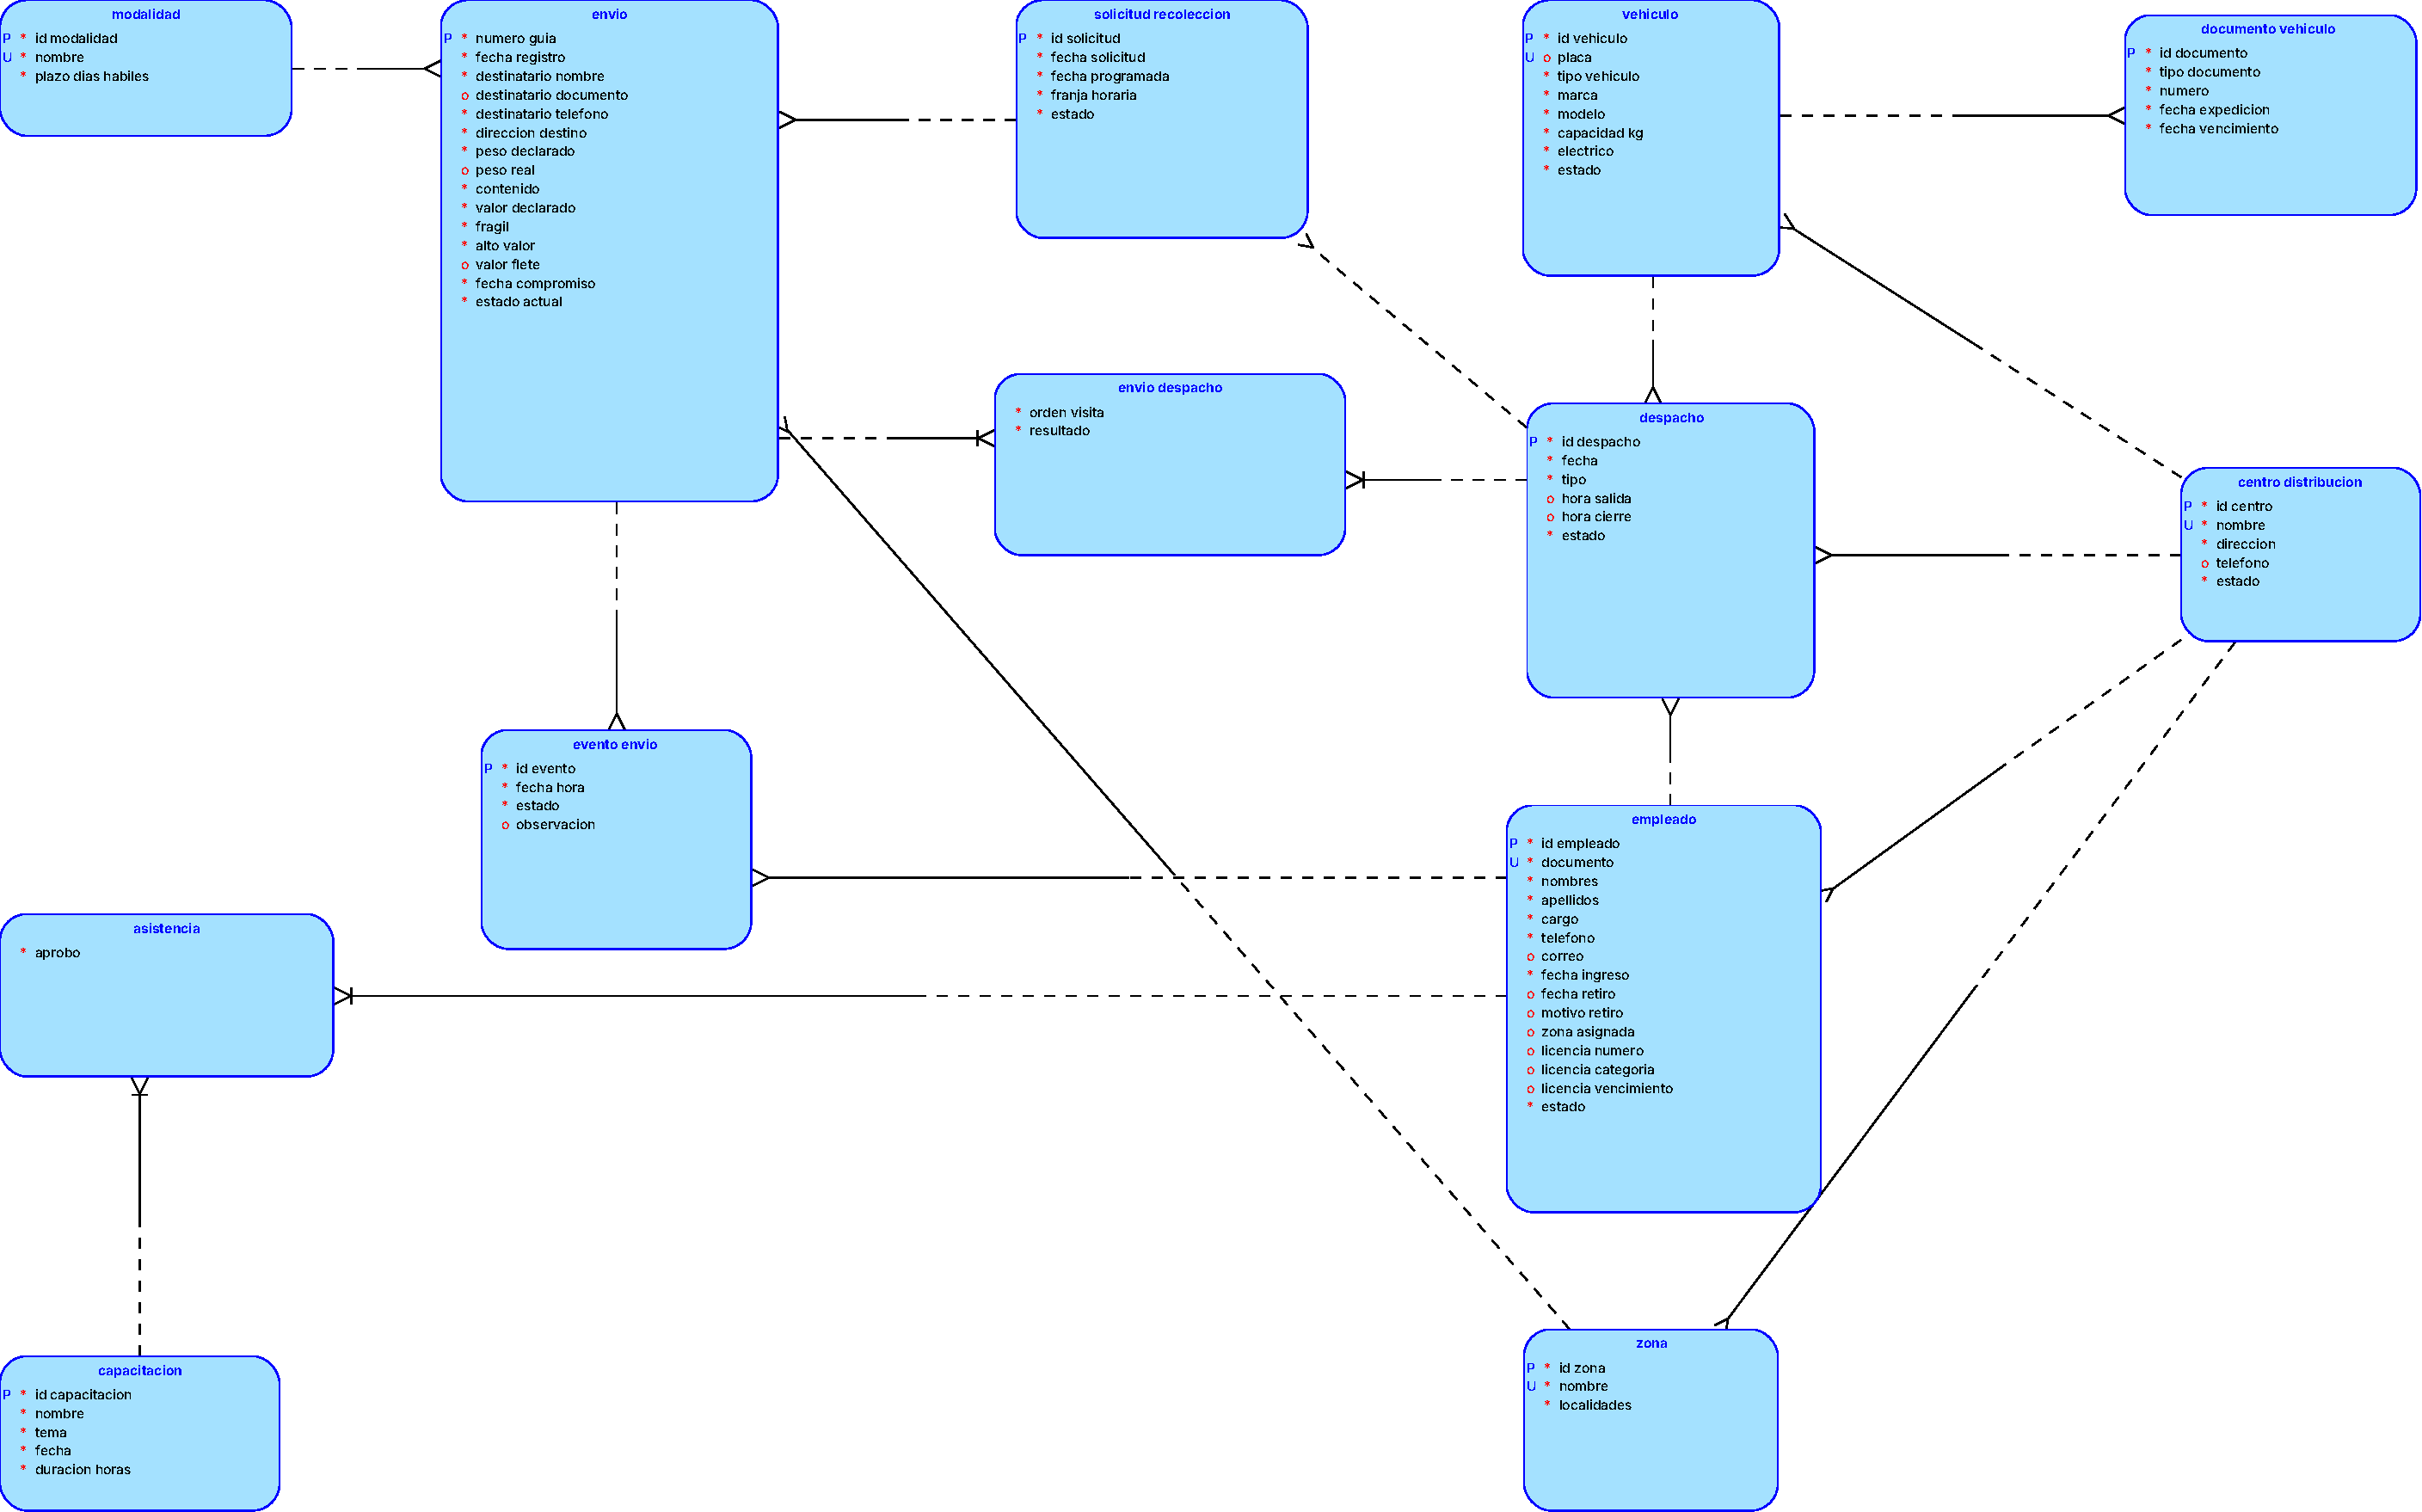
\includegraphics{figuras/datamodeler/dm_U2.pdf}
}
\caption{Vista U2 en Data Modeler (subvista del prediseño).}
\label{fig:dmU2}
\end{figure}
\par}
\end{landscape}

\begin{landscape}
{\singlespacing
\begin{figure}[p]
\centering
\adjustbox{max width=22.5cm, max totalheight=14.6cm}{%%
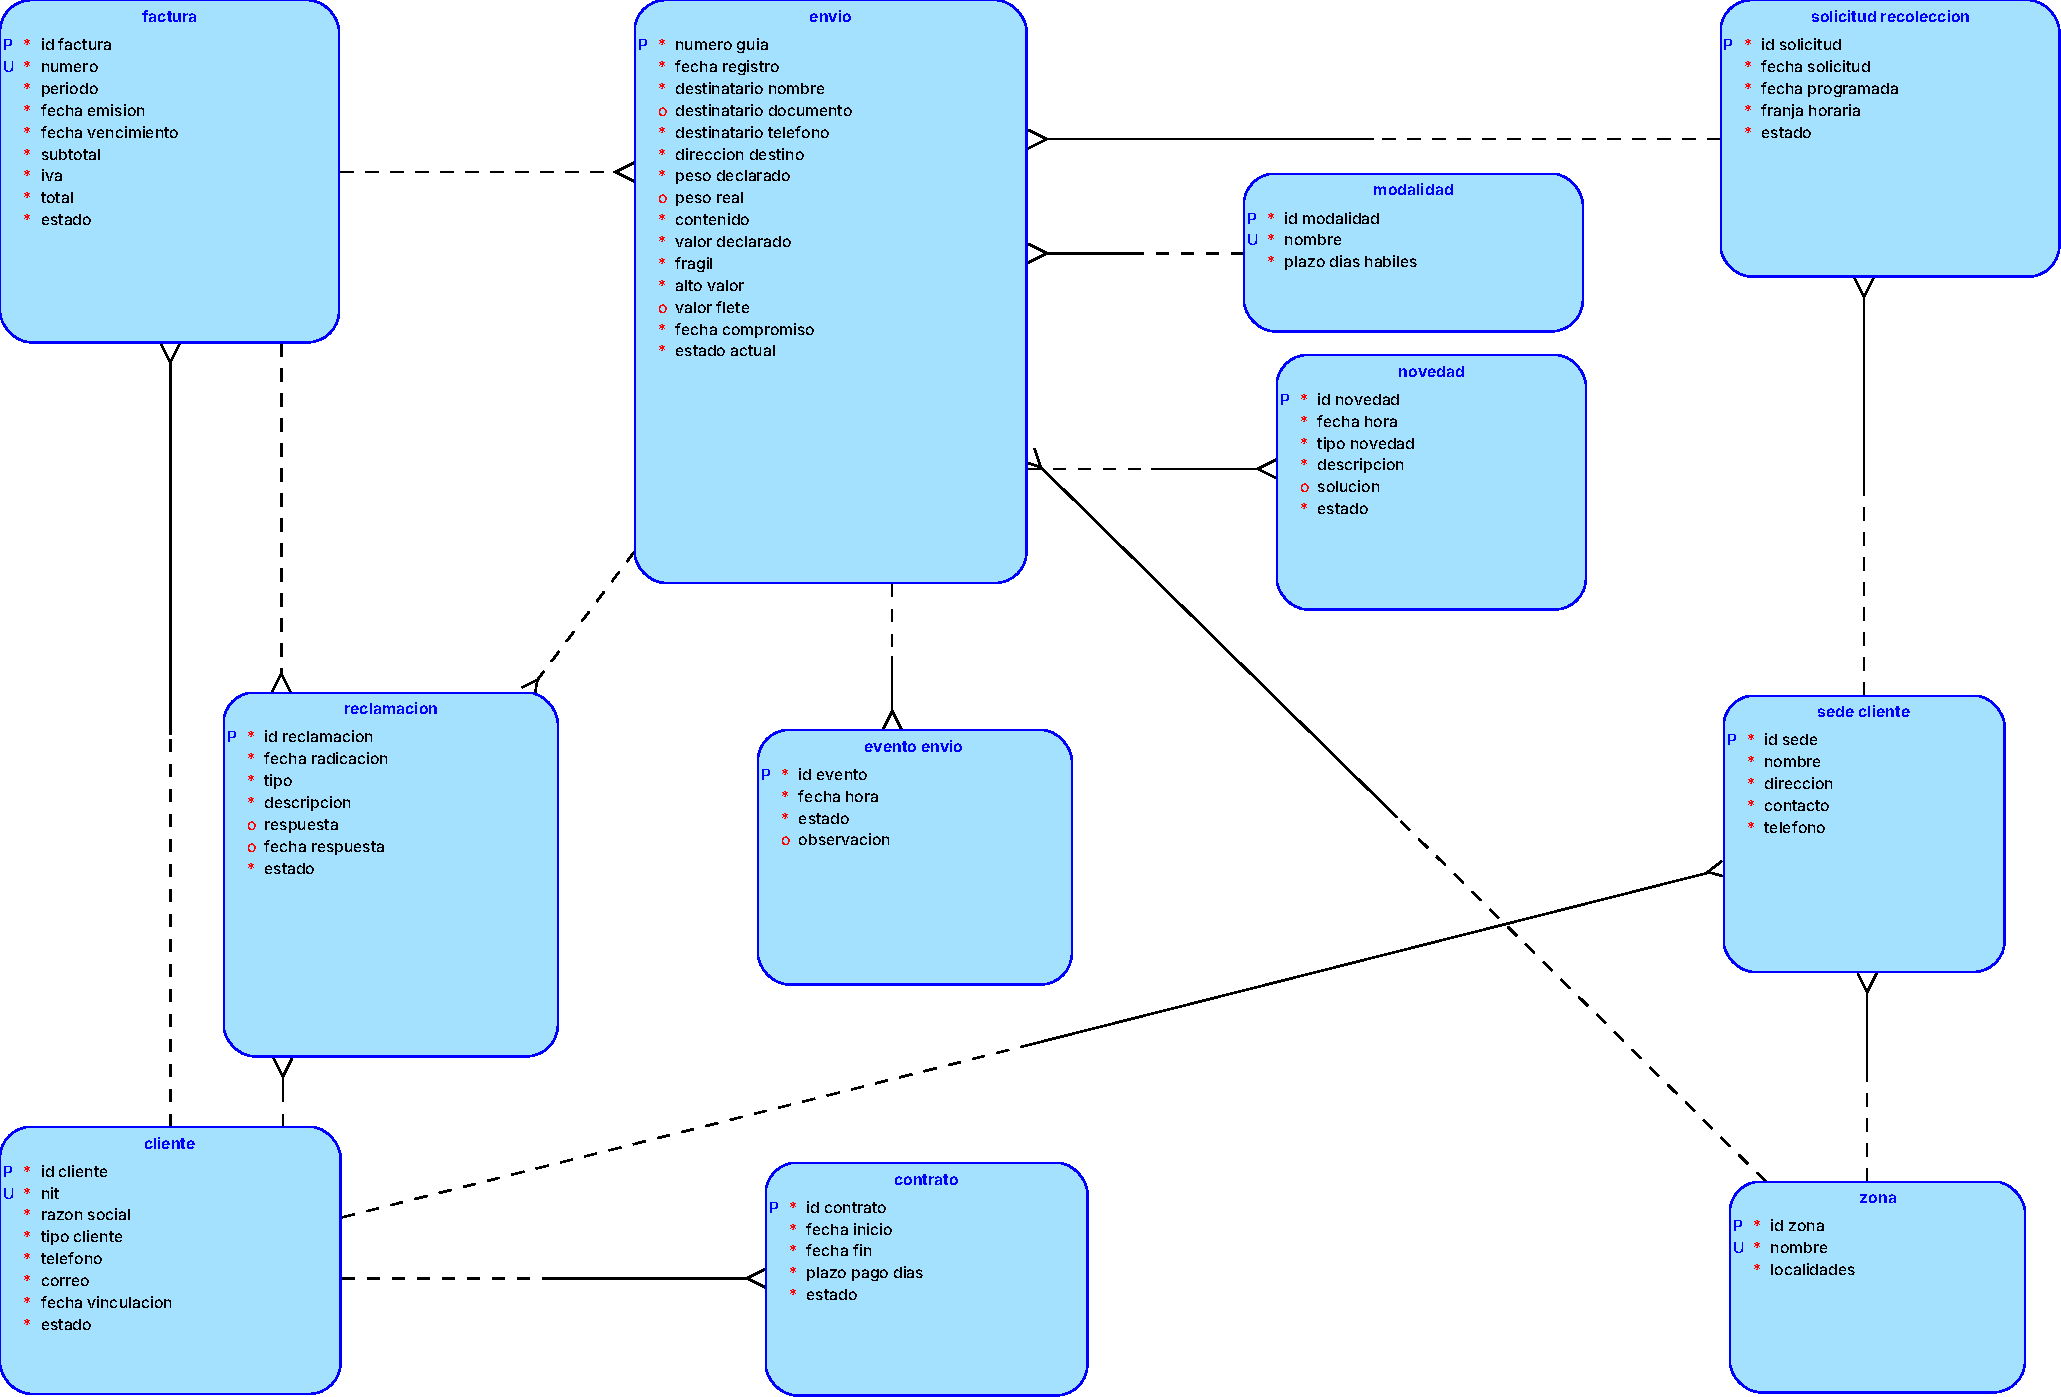
\includegraphics{figuras/datamodeler/dm_U3.pdf}
}
\caption{Vista U3 en Data Modeler (subvista del prediseño).}
\label{fig:dmU3}
\end{figure}
\par}
\end{landscape}

{\singlespacing
\begin{figure}[!htb]
\centering
\adjustbox{max width=\linewidth}{%%
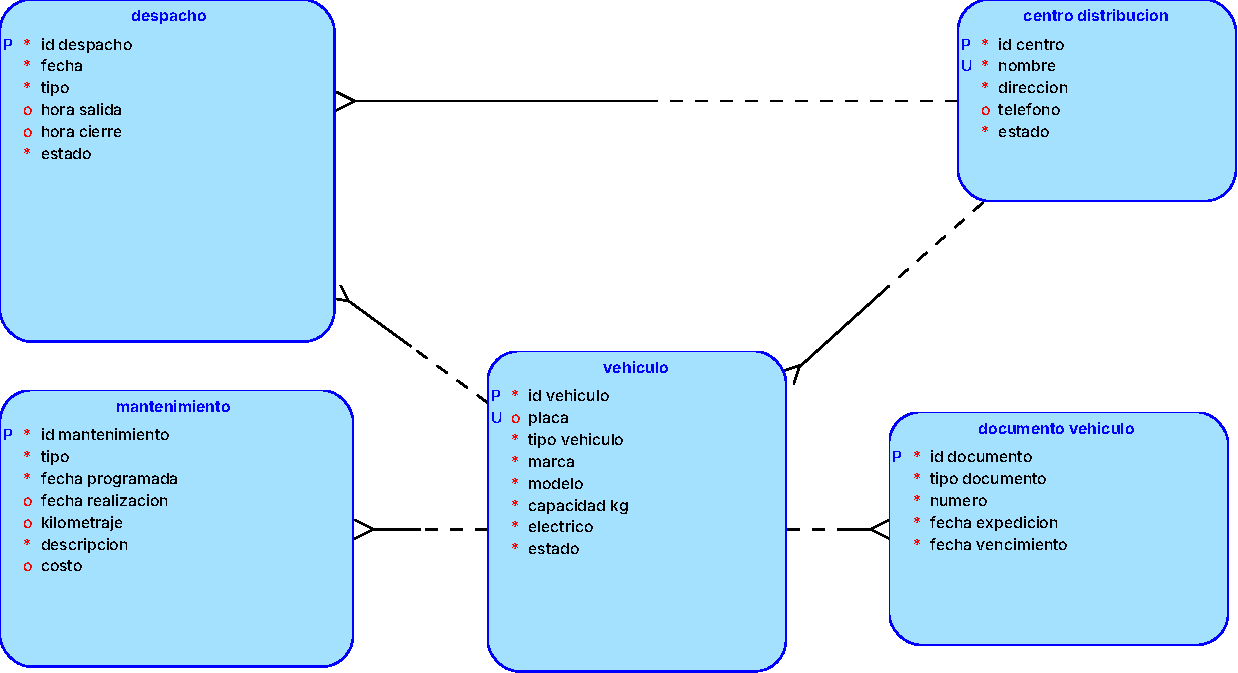
\includegraphics[height=0.62\textheight,width=\linewidth,keepaspectratio]{figuras/datamodeler/dm_U5.pdf}
}
\caption{Vista U5 en Data Modeler (subvista del prediseño).}
\label{fig:dmU5}
\end{figure}
\par}

{\singlespacing
\begin{figure}[!htb]
\centering
\adjustbox{max width=\linewidth}{%%
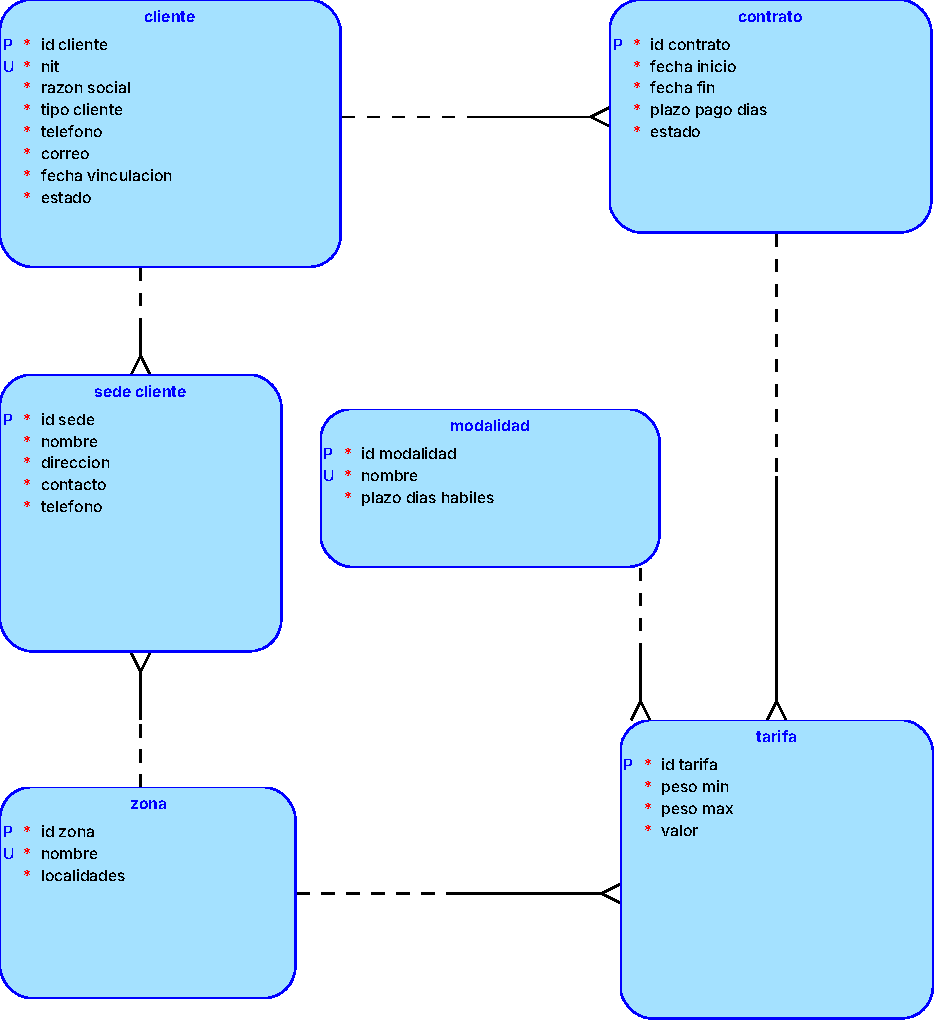
\includegraphics[height=0.62\textheight,width=\linewidth,keepaspectratio]{figuras/datamodeler/dm_U6.pdf}
}
\caption{Vista U6 en Data Modeler (subvista del prediseño).}
\label{fig:dmU6}
\end{figure}
\par}

{\singlespacing
\begin{figure}[!htb]
\centering
\adjustbox{max width=\linewidth}{%%
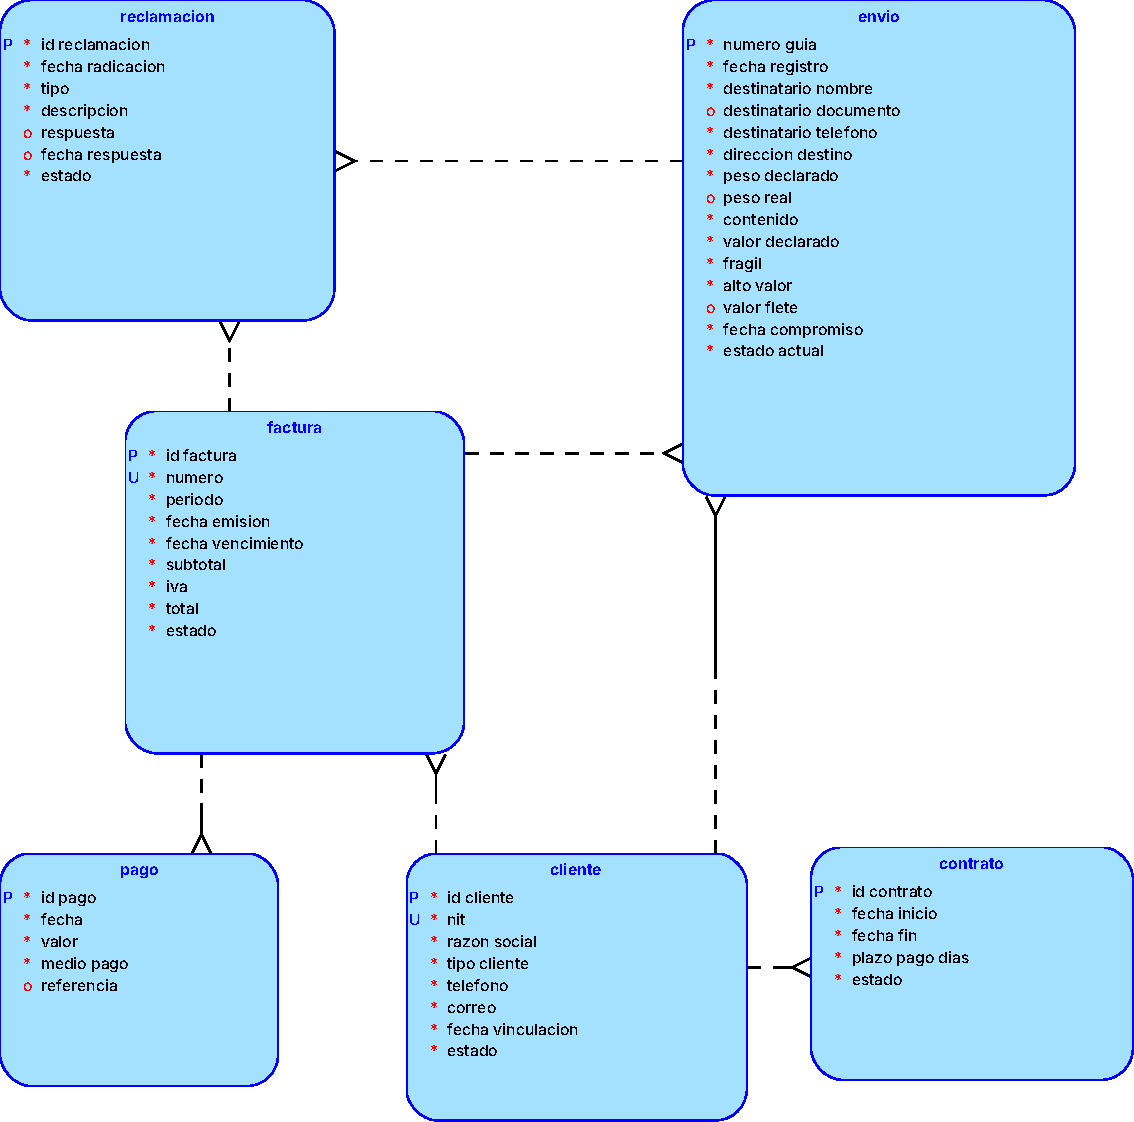
\includegraphics[height=0.62\textheight,width=\linewidth,keepaspectratio]{figuras/datamodeler/dm_U7.pdf}
}
\caption{Vista U7 en Data Modeler (diseño propio).}
\label{fig:dmU7}
\end{figure}
\par}

{\singlespacing
\begin{figure}[!htb]
\centering
\adjustbox{max width=\linewidth}{%%
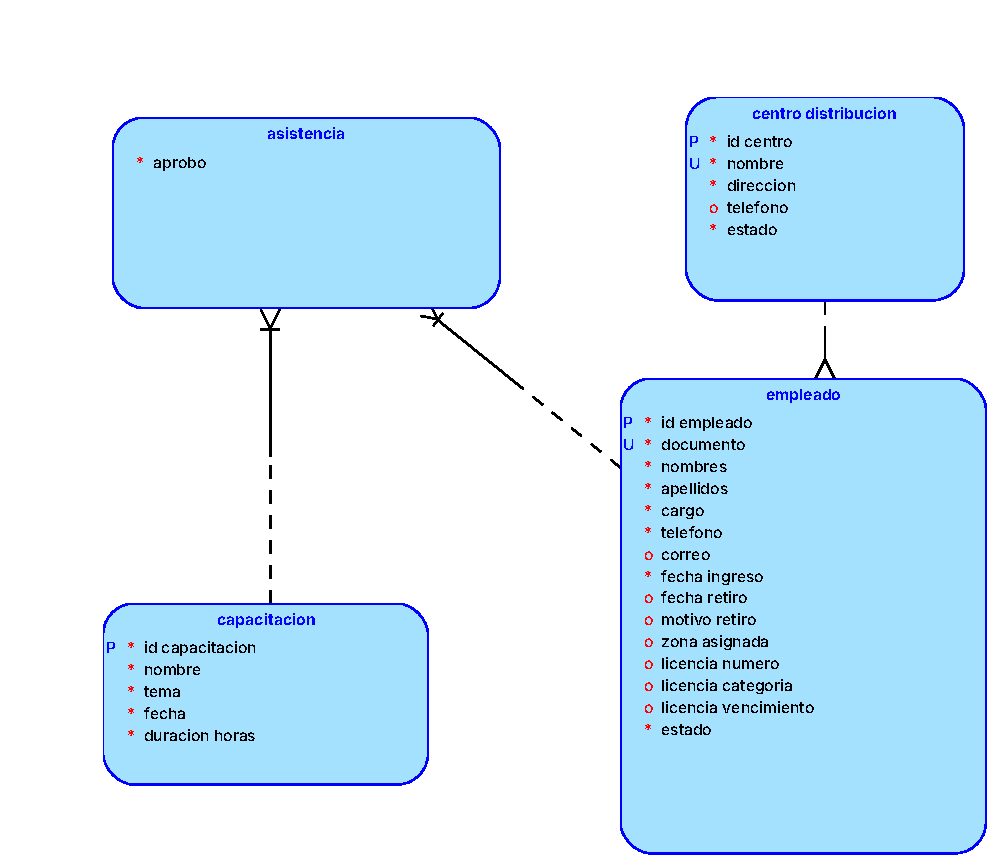
\includegraphics[height=0.62\textheight,width=\linewidth,keepaspectratio]{figuras/datamodeler/dm_U8.pdf}
}
\caption{Vista U8 en Data Modeler (subvista del prediseño).}
\label{fig:dmU8}
\end{figure}
\par}

\begin{landscape}
{\singlespacing
\begin{figure}[p]
\centering
\adjustbox{max width=22.5cm, max totalheight=14.6cm}{%%
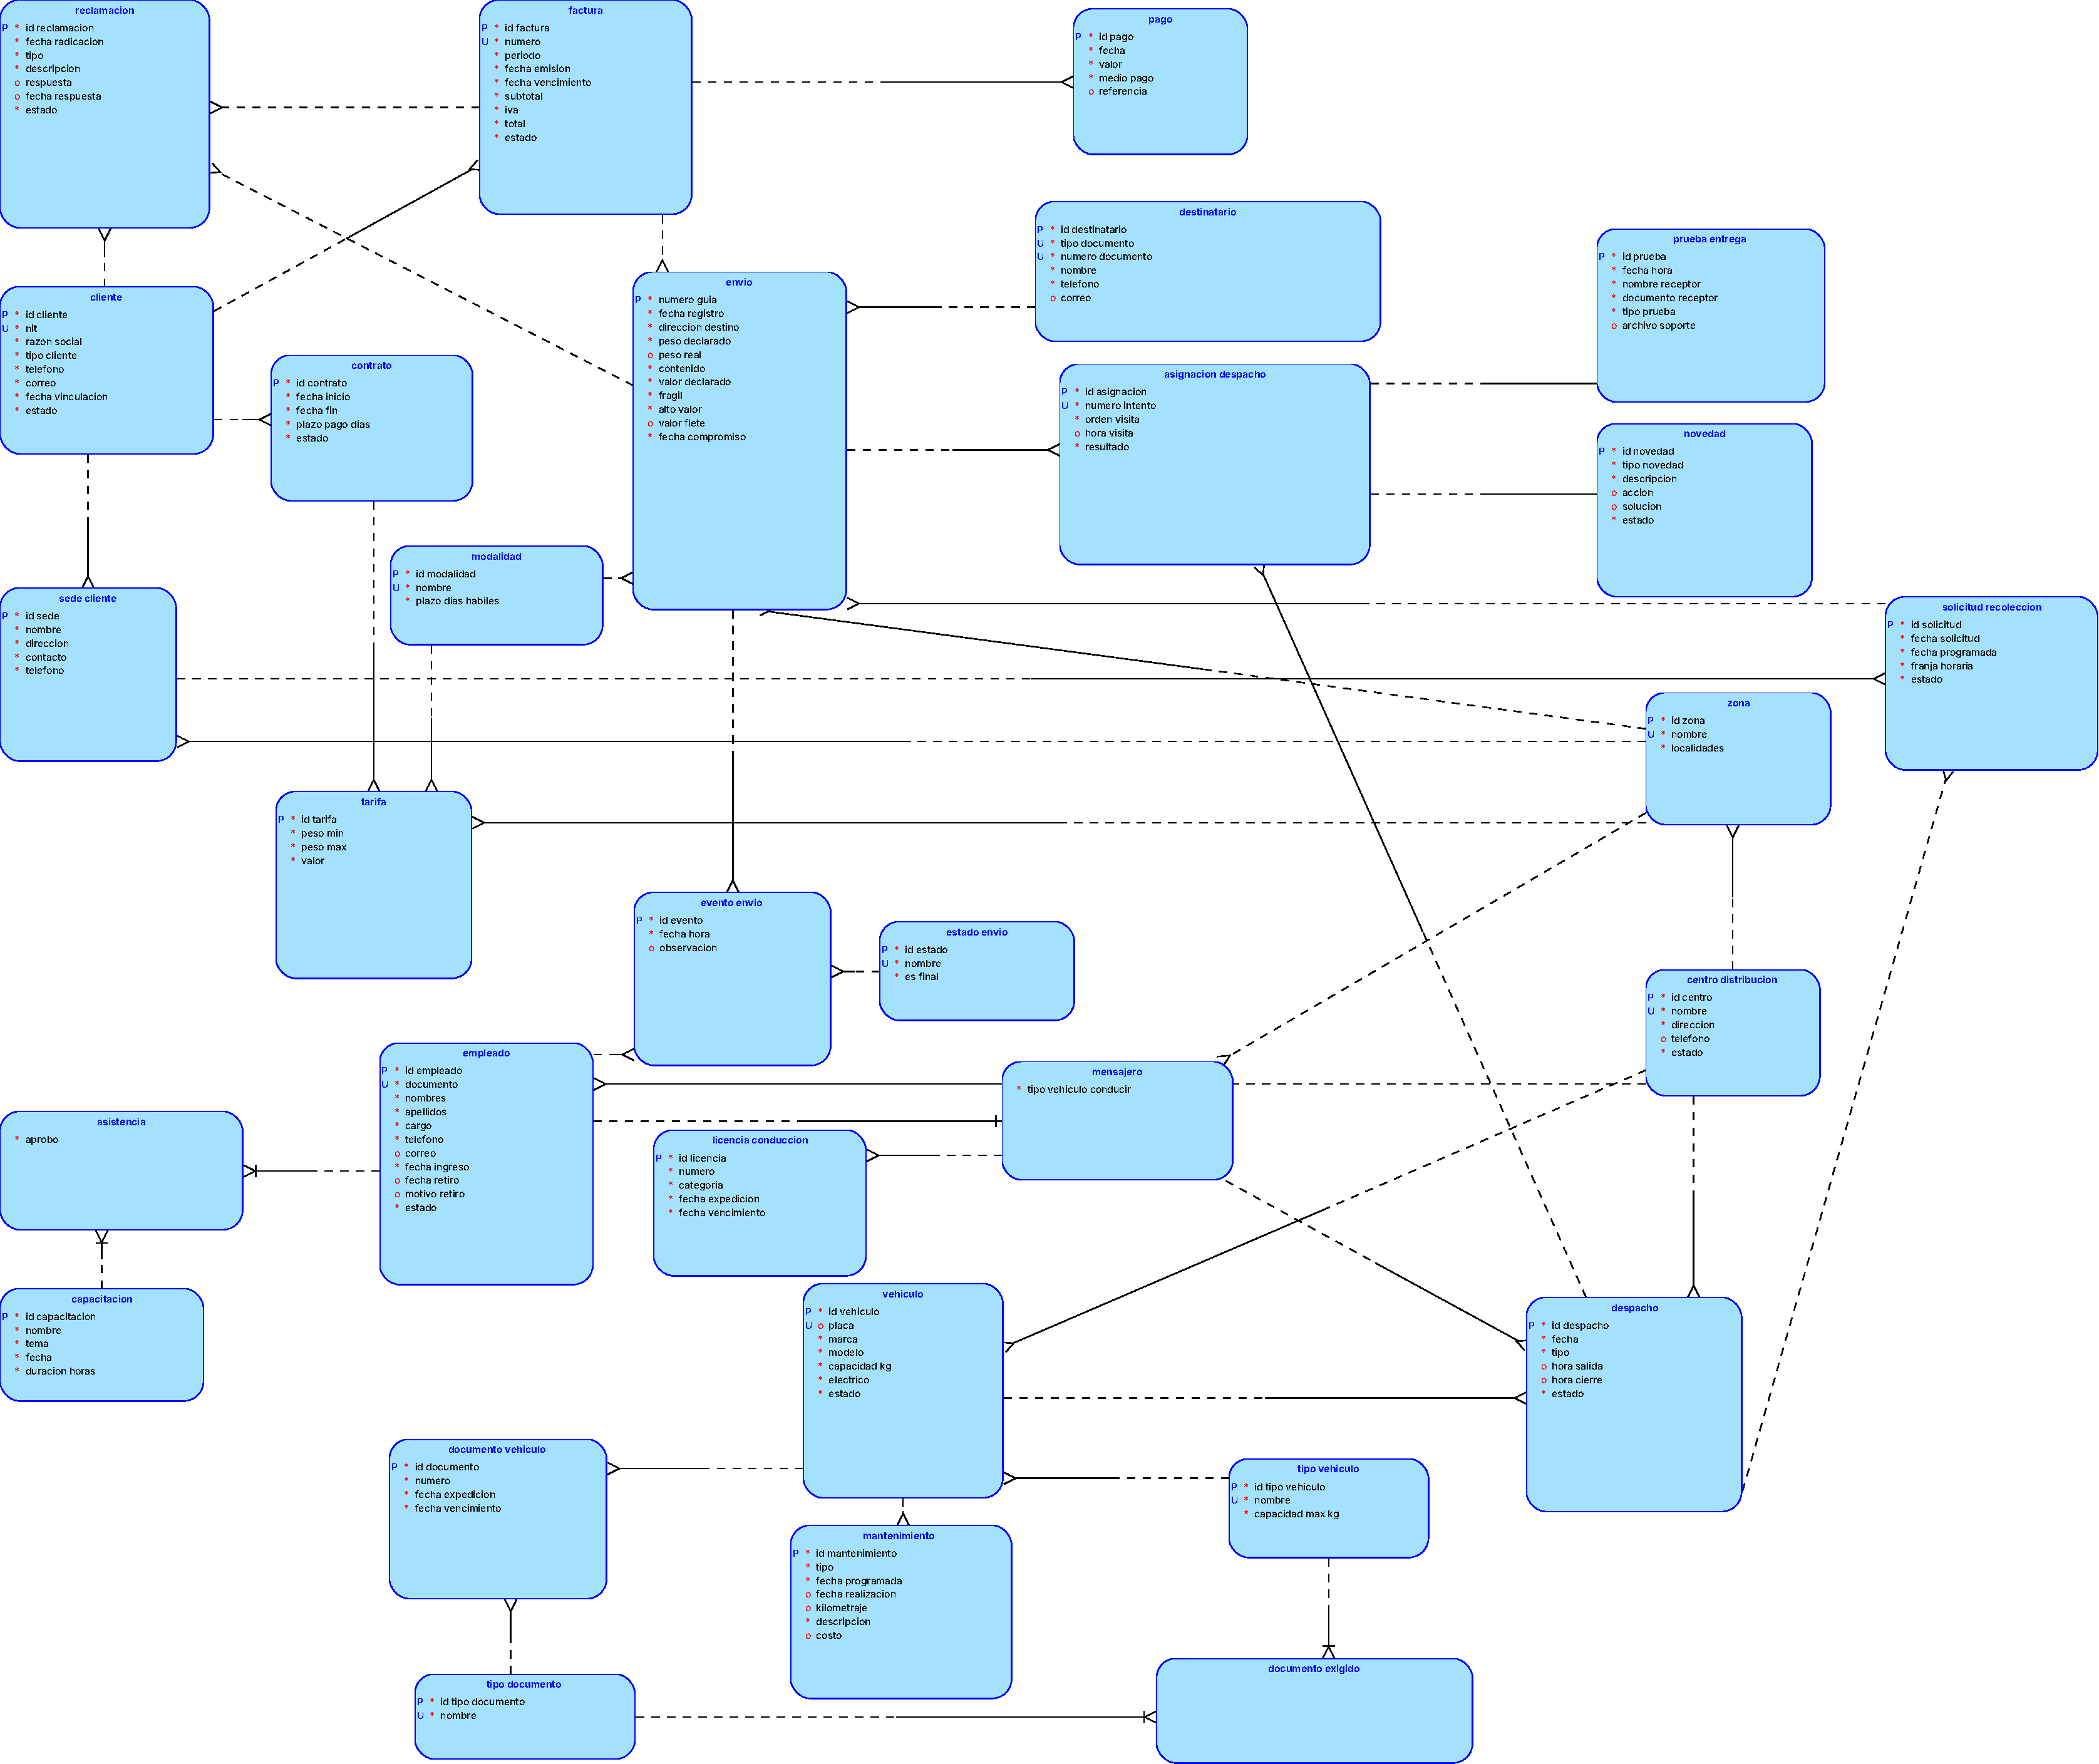
\includegraphics{figuras/datamodeler/dm_modelo_ajustado.pdf}
}
\caption{Modelo ajustado en Data Modeler (diseño completo, 30 entidades).}
\label{fig:dmajustado}
\end{figure}
\par}
\end{landscape}

\newpage

%======================================================================
%  Anexo D - Diccionario de datos generado en la herramienta CASE
%======================================================================

\section{Diccionario de datos generado en la herramienta CASE}
\label{anx:dmdiccionario}

Este anexo es la evidencia de que el diccionario de datos de la
sección~\ref{sec:diccionario} coincide con el modelo implementado en
Oracle SQL Developer Data Modeler. El reporte se generó con
\textit{File $\rightarrow$ Reports}, con una plantilla personalizada
(\textit{Diccionario}) de cuatro secciones por tabla: nombre y
\textit{Comment in RDBMS}, restricciones de verificación de la tabla,
claves primaria y únicas con sus columnas, y claves foráneas con la
columna referenciada.

El reporte se comparó con el modelo relacional del capítulo 4. Coinciden las
19 tablas, la descripción de cada una, las 32 claves primarias y únicas
(19 y 13) con sus columnas, las 27 claves foráneas con la columna que
referencian y las 7 restricciones de verificación que involucran varias
columnas. Las 26 restricciones de una sola columna (listas de valores y
rangos) la herramienta las guarda en la propia columna, por eso no
aparecen en la tabla~\ref{tab:dmdiccionario}. El detalle de cada
columna (tipo, nulos, valor por defecto y descripción) está en la
tabla~\ref{tab:diccionario}.

{\scriptsize
\begin{longtable}{|L{3.0cm}|L{3.9cm}|L{3.8cm}|L{3.6cm}|}
\caption{Reporte de tablas del módulo generado en Data Modeler.}
\label{tab:dmdiccionario}\\
\hline
\textbf{Tabla y descripción} & \textbf{Claves primaria y únicas (columnas)} & \textbf{Claves foráneas (columna referenciada)} & \textbf{Restricciones de verificación} \\ \hline
\endfirsthead
\hline
\textbf{Tabla y descripción} & \textbf{Claves primaria y únicas (columnas)} & \textbf{Claves foráneas (columna referenciada)} & \textbf{Restricciones de verificación} \\ \hline
\endhead
\textbf{ASIGNACION\_DESPACHO} \newline Cada intento de un envío en un despacho. & \textbf{ASIGNACION\_PK} (ID\_ASIGNACION) \newline \textbf{ASIGNACION\_ENVIO\_DESP\_UK} (NUMERO\_GUIA, ID\_DESPACHO) \newline \textbf{ASIGNACION\_INTENTO\_UK} (NUMERO\_GUIA, NUMERO\_INTENTO) & ASIGNACION\_DESPACHO\_FK (ID\_DESPACHO) \newline ASIGNACION\_ENVIO\_FK (NUMERO\_GUIA) & -- \\ \hline
\textbf{CENTRO\_DISTRIBUCION} \newline Centro donde se reciben, clasifican y despachan los envíos. & \textbf{CENTRO\_PK} (ID\_CENTRO) \newline \textbf{CENTRO\_NOMBRE\_UK} (NOMBRE) & -- & -- \\ \hline
\textbf{CLIENTE} \newline Empresa que contrata el servicio. & \textbf{CLIENTE\_PK} (ID\_CLIENTE) \newline \textbf{CLIENTE\_NIT\_UK} (NIT) & -- & -- \\ \hline
\textbf{DESPACHO} \newline Salida de un mensajero con un vehículo. & \textbf{DESPACHO\_PK} (ID\_DESPACHO) & DESPACHO\_CENTRO\_FK (ID\_CENTRO) \newline DESPACHO\_MENSAJERO\_FK (ID\_EMPLEADO) \newline DESPACHO\_VEHICULO\_FK (ID\_VEHICULO) & DESPACHO\_HORAS\_CK: la hora de cierre, si existe, es posterior a la de salida \\ \hline
\textbf{DESTINATARIO} \newline Persona que recibe los envíos. & \textbf{DESTINATARIO\_PK} (ID\_DESTINATARIO) \newline \textbf{DESTINATARIO\_DOCUMENTO\_UK} (TIPO\_DOCUMENTO, NUMERO\_DOCUMENTO) & -- & -- \\ \hline
\textbf{EMPLEADO} \newline Persona vinculada a la empresa. & \textbf{EMPLEADO\_PK} (ID\_EMPLEADO) \newline \textbf{EMPLEADO\_DOCUMENTO\_UK} (DOCUMENTO) & EMPLEADO\_CENTRO\_FK (ID\_CENTRO) & EMPLEADO\_RETIRO\_CK: la fecha de retiro, si existe, no es anterior a la de ingreso \\ \hline
\textbf{ENVIO} \newline Paquete o documento identificado por su guía. & \textbf{ENVIO\_PK} (NUMERO\_GUIA) & ENVIO\_DESTINATARIO\_FK (ID\_DESTINATARIO) \newline ENVIO\_MODALIDAD\_FK (ID\_MODALIDAD) \newline ENVIO\_SOLICITUD\_FK (ID\_SOLICITUD) \newline ENVIO\_ZONA\_FK (ID\_ZONA) & ENVIO\_COMPROMISO\_CK: la fecha de compromiso no es anterior a la de registro \newline ENVIO\_PESOS\_CK: el peso declarado y el peso real, si existe, son mayores que 0 \newline ENVIO\_VALOR\_CK: el valor declarado no es negativo y el flete, si existe, es mayor que 0 \\ \hline
\textbf{ESTADO\_ENVIO} \newline Catálogo de estados del envío. & \textbf{ESTADO\_ENVIO\_PK} (ID\_ESTADO) \newline \textbf{ESTADO\_ENVIO\_NOMBRE\_UK} (NOMBRE) & -- & -- \\ \hline
\textbf{EVENTO\_ENVIO} \newline Cada cambio de estado de un envío. & \textbf{EVENTO\_PK} (ID\_EVENTO) & EVENTO\_EMPLEADO\_FK (ID\_EMPLEADO) \newline EVENTO\_ENVIO\_FK (NUMERO\_GUIA) \newline EVENTO\_ESTADO\_FK (ID\_ESTADO) & -- \\ \hline
\textbf{MENSAJERO} \newline Empleado que sale a ruta (subtipo de EMPLEADO). & \textbf{MENSAJERO\_PK} (ID\_EMPLEADO) & MENSAJERO\_EMPLEADO\_FK (ID\_EMPLEADO) \newline MENSAJERO\_TIPO\_VEH\_FK (ID\_TIPO\_VEHICULO) \newline MENSAJERO\_ZONA\_FK (ID\_ZONA) & -- \\ \hline
\textbf{MODALIDAD} \newline Tipo de servicio según el tiempo de entrega. & \textbf{MODALIDAD\_PK} (ID\_MODALIDAD) \newline \textbf{MODALIDAD\_NOMBRE\_UK} (NOMBRE) & -- & -- \\ \hline
\textbf{NOVEDAD} \newline Situación que impidió la entrega en un intento. & \textbf{NOVEDAD\_PK} (ID\_NOVEDAD) \newline \textbf{NOVEDAD\_ASIGNACION\_UK} (ID\_ASIGNACION) & NOVEDAD\_ASIGNACION\_FK (ID\_ASIGNACION) & -- \\ \hline
\textbf{PRUEBA\_ENTREGA} \newline Constancia de recibo de una entrega o devolución. & \textbf{PRUEBA\_PK} (ID\_PRUEBA) \newline \textbf{PRUEBA\_ASIGNACION\_UK} (ID\_ASIGNACION) & PRUEBA\_ASIGNACION\_FK (ID\_ASIGNACION) & -- \\ \hline
\textbf{RECLAMACION} \newline Inconformidad de un cliente. & \textbf{RECLAMACION\_PK} (ID\_RECLAMACION) & RECLAMACION\_CLIENTE\_FK (ID\_CLIENTE) \newline RECLAMACION\_ENVIO\_FK (NUMERO\_GUIA) & RECLAMACION\_RESP\_CK: la fecha de respuesta, si existe, no es anterior a la de radicación \\ \hline
\textbf{SEDE\_CLIENTE} \newline Punto de recolección de un cliente. & \textbf{SEDE\_PK} (ID\_SEDE) & SEDE\_CLIENTE\_FK (ID\_CLIENTE) \newline SEDE\_ZONA\_FK (ID\_ZONA) & -- \\ \hline
\textbf{SOLICITUD\_RECOLECCION} \newline Pedido de recolección en una sede del cliente. & \textbf{SOLICITUD\_PK} (ID\_SOLICITUD) & SOLICITUD\_DESPACHO\_FK (ID\_DESPACHO) \newline SOLICITUD\_SEDE\_FK (ID\_SEDE) & SOLICITUD\_FECHAS\_CK: la fecha programada no es anterior a la de solicitud \\ \hline
\textbf{TIPO\_VEHICULO} \newline Catálogo de tipos de vehículo. & \textbf{TIPO\_VEHICULO\_PK} (ID\_TIPO\_VEHICULO) \newline \textbf{TIPO\_VEHICULO\_NOMBRE\_UK} (NOMBRE) & -- & -- \\ \hline
\textbf{VEHICULO} \newline Vehículo de la flota. & \textbf{VEHICULO\_PK} (ID\_VEHICULO) \newline \textbf{VEHICULO\_PLACA\_UK} (PLACA) & VEHICULO\_CENTRO\_FK (ID\_CENTRO) \newline VEHICULO\_TIPO\_FK (ID\_TIPO\_VEHICULO) & -- \\ \hline
\textbf{ZONA} \newline Sector de la ciudad atendido por un centro. & \textbf{ZONA\_PK} (ID\_ZONA) \newline \textbf{ZONA\_NOMBRE\_UK} (NOMBRE) & ZONA\_CENTRO\_FK (ID\_CENTRO) & -- \\ \hline
\end{longtable}
}

\newpage

%======================================================================
%  Anexo E - Diagramas del modulo en notacion de Chen (draw.io)
%======================================================================

\section{Diagramas del módulo en notación de Chen}
\label{anx:chen}

En el cuerpo del documento los diagramas del módulo se presentan como
quedaron en Oracle SQL Developer Data Modeler. Este anexo conserva las
versiones elaboradas en draw.io con la notación de Chen, que muestran lo que la notación
Barker de la herramienta omite: el nombre de cada relación, su
participación (mín,máx) y, en el modelo relacional, la tabla a la que
apunta cada clave foránea. Ambas versiones representan el mismo modelo y
se verificaron entre sí relación por relación.

La figura~\ref{fig:vistaU4chen} corresponde a la vista U4 del mensajero
(figura~\ref{fig:vistaU4}); en ella la asignación de un envío a un
despacho es la relación N:M \textit{contiene}, con los atributos orden de
visita y resultado.

{\singlespacing
\begin{figure}[!htb]
\centering
\adjustbox{max width=\linewidth, max totalheight=0.42\textheight}{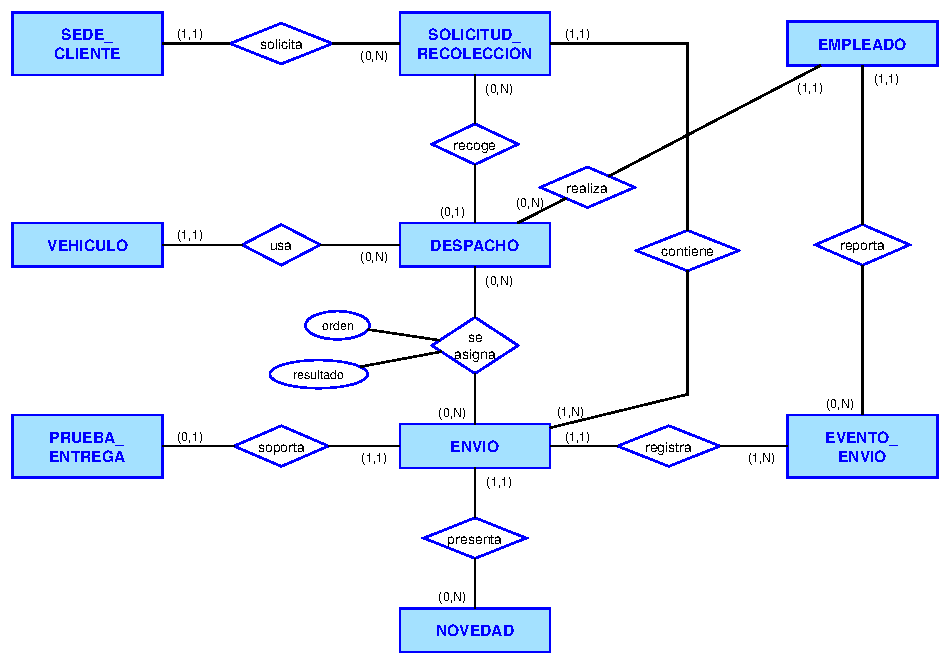
\includegraphics{figuras/er/M_U4.pdf}}
\caption{Vista U4: mensajero, en notación de Chen.}
\label{fig:vistaU4chen}
\end{figure}
\par}

La figura~\ref{fig:erfinal} es el modelo Entidad-Relación ajustado del
módulo (figura~\ref{fig:dmlogico}): 19 entidades, 26 relaciones con
nombre y la especialización parcial de EMPLEADO en MENSAJERO.

La figura~\ref{fig:relacional} es el modelo relacional del módulo
(figura~\ref{fig:dmrelacional}). En cada tabla, \texttt{P} marca la
clave primaria, \texttt{F} una clave foránea (con la tabla a la que
apunta), \texttt{PF} una columna que es ambas, \texttt{U} un valor
único, \texttt{*} una columna obligatoria y \texttt{o} una opcional.

\begin{landscape}
{\singlespacing
\begin{figure}[p]
\centering
\adjustbox{max width=22.5cm, max totalheight=14.6cm}{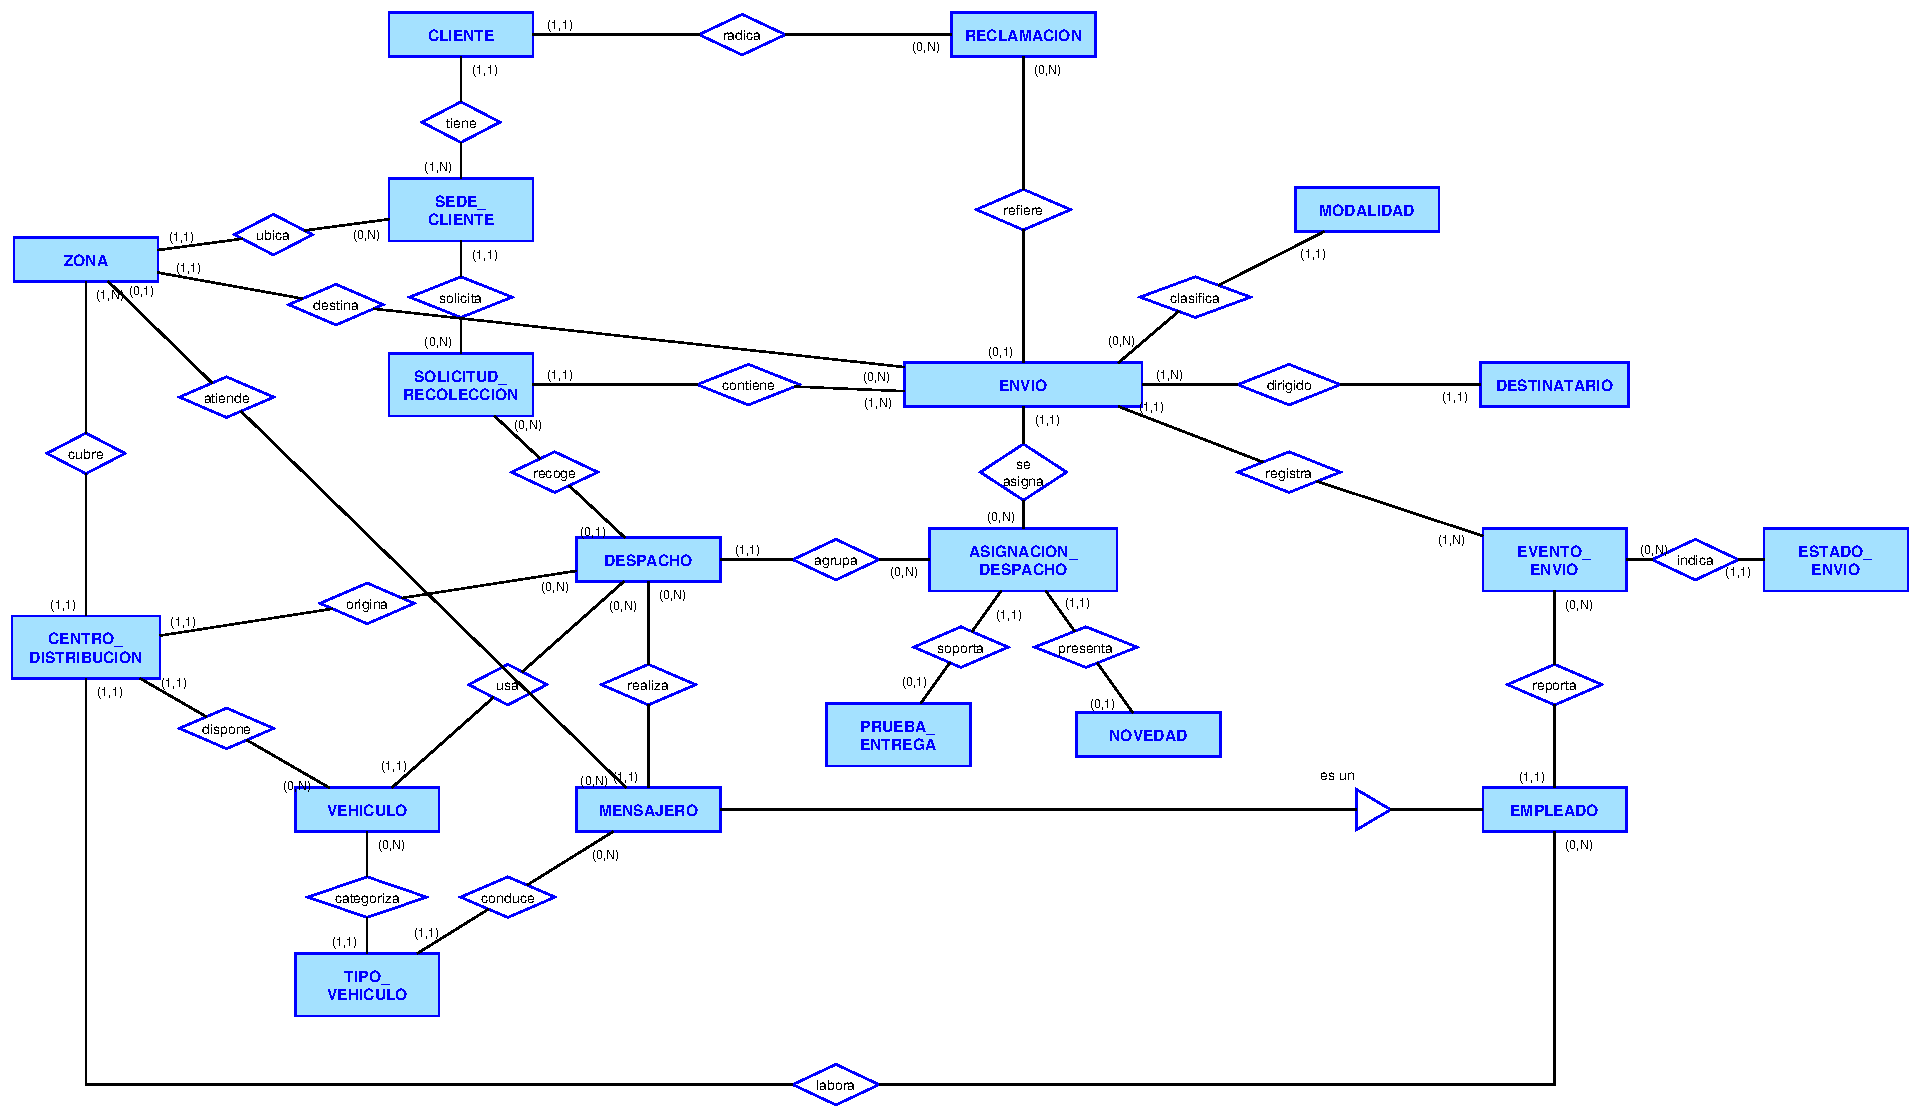
\includegraphics{figuras/er/M_final.pdf}}
\caption{Modelo Entidad-Relación ajustado del módulo de operación de envíos, en notación de Chen.}
\label{fig:erfinal}
\end{figure}
\par}
\end{landscape}

\begin{landscape}
{\singlespacing
\begin{figure}[p]
\centering
\adjustbox{max width=22.5cm, max totalheight=14.6cm}{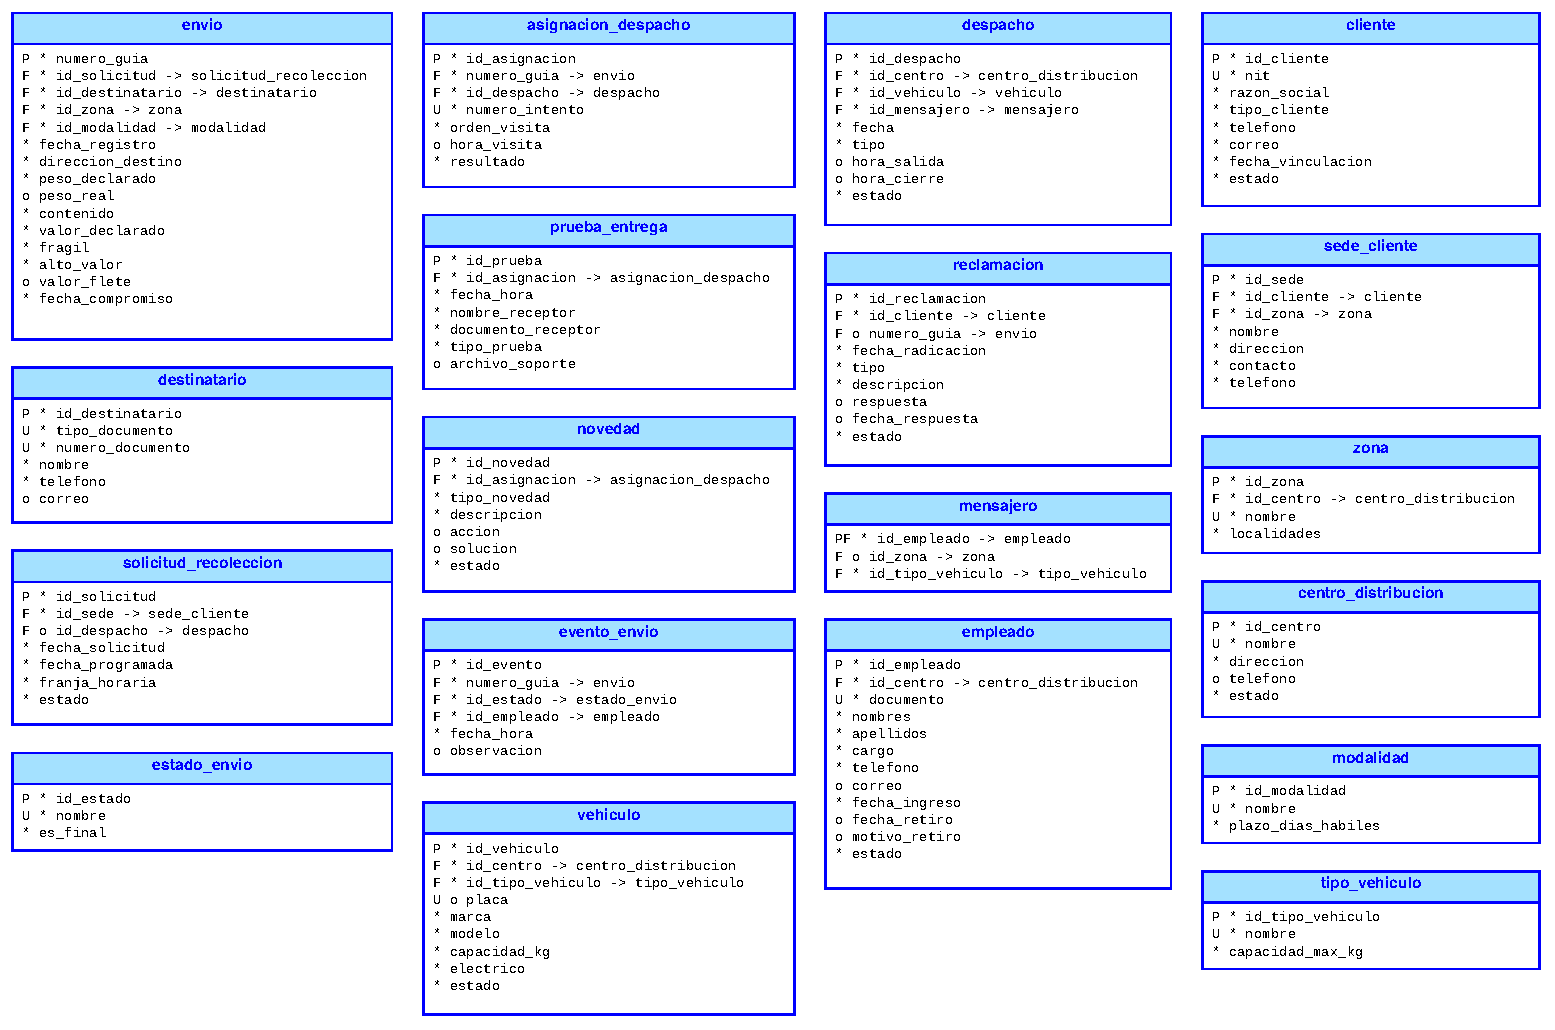
\includegraphics{figuras/er/M_relacional.pdf}}
\caption{Modelo relacional del módulo de operación de envíos, elaborado en draw.io.}
\label{fig:relacional}
\end{figure}
\par}
\end{landscape}


\end{document}
